\chapter{The July 2026 Estimation Campaign: Tightly-Coupled Multisensor Fusion}
\label{ch:fusion}

This chapter documents the second major engineering campaign on the platform
(July 3--7, 2026), which extended the mission-control system of the previous
chapters with a precision $(x,y,z)$ state-estimation stack, hardened the
sensor-integrity chain against three failure modes observed live, upgraded the
operator web platform, and integrated one hardware modification (rigid
high-performance wheels). Every parameter cited below is justified by its
measured contribution to drift reduction, and every remaining placeholder is
explicitly registered in Section~\ref{sec:openitems}.

%=============================================================================
\section{Estimation architecture}
\label{sec:fusionarch}

\subsection{From mission control to metric estimation}
The system of Chapters 3--5 estimated pose from wheel odometry alone, reset at
each beacon. The campaign objective was to replace this dead-reckoning core
with a fused estimate whose drift is \emph{bounded and measured}, while keeping
the beacon-reset ritual as a world-frame anchor. Two estimators were deployed,
switchable live:

\begin{itemize}
  \item \textbf{MINS}~\cite{lee2023mins,lee2025minsjfr}, the primary
        estimator: a tightly-coupled Multi-State Constraint Kalman Filter
        (MSCKF) fusing the onboard IMU, the two front wheel encoders and the
        D455 stereo infrared pair, with online calibration of every sensor's
        extrinsics and time offset.
  \item \textbf{OpenVINS}~\cite{geneva2020openvins}, the reference
        visual-inertial estimator (IMU + stereo only), used for A/B comparison
        and camera-calibration validation.
\end{itemize}

\subsection{Why tightly-coupled MSCKF, and not a decoupled EKF}
\label{sec:whymsckf}
A decoupled fusion stack (e.g.\ \code{robot\_localization}) fuses
\emph{poses} already estimated by upstream nodes, treating them as independent
measurements. On this platform the visual and wheel odometries share the same
IMU and the same clock: their errors are strongly correlated, and a decoupled
filter double-counts the shared information, producing overconfident
covariances: the statistical root of divergence. The MSCKF instead fuses
\emph{raw measurements} in a single state vector
\begin{equation}
\mathbf{x} \;=\; \big[\,
{}^{I}_{G}\bar{q},\;
{}^{G}\mathbf{p}_{I},\;
{}^{G}\mathbf{v}_{I},\;
\mathbf{b}_{g},\;
\mathbf{b}_{a}
\,\big|\,
\mathbf{x}_{c_1},\dots,\mathbf{x}_{c_N}
\,\big|\,
\boldsymbol{\theta}_{\mathrm{calib}}
\big],
\label{eq:state}
\end{equation}
where ${}^{I}_{G}\bar{q}$ is the orientation quaternion,
${}^{G}\mathbf{p}_{I}, {}^{G}\mathbf{v}_{I}$ position and velocity in the
global frame, $\mathbf{b}_g, \mathbf{b}_a$ the slowly-varying gyroscope and
accelerometer biases, $\mathbf{x}_{c_i}$ a sliding window of $N$ historical
pose \emph{clones}, and $\boldsymbol{\theta}_{\mathrm{calib}}$ the online
calibration states (camera--IMU extrinsics and time offset, wheel extrinsics).

\paragraph{Propagation.} Each IMU sample (measured rate
$\boldsymbol{\omega}_m$, specific force $\mathbf{a}_m$, at
$\sim$80\,Hz on this platform) propagates the state through the standard
inertial kinematics
\begin{IEEEeqnarray}{rCl}
{}^{I}_{G}\dot{\bar{q}} &=& \tfrac{1}{2}\,
  \boldsymbol{\Omega}\!\big(\boldsymbol{\omega}_m - \mathbf{b}_g - \mathbf{n}_g\big)\,
  {}^{I}_{G}\bar{q}, \\
{}^{G}\dot{\mathbf{v}}_{I} &=&
  {}^{G}_{I}\mathbf{R}\,\big(\mathbf{a}_m - \mathbf{b}_a - \mathbf{n}_a\big)
  + {}^{G}\mathbf{g}, \qquad
{}^{G}\dot{\mathbf{p}}_{I} \;=\; {}^{G}\mathbf{v}_{I},
\label{eq:imukin}
\end{IEEEeqnarray}
with $\mathbf{n}_g, \mathbf{n}_a$ white noises whose densities were identified
on \emph{this unit} by Allan-variance analysis
(\code{imu\_utils}): $\sigma_a = 2.33\times10^{-2}$, $\sigma_{ba} =
8.93\times10^{-4}$, $\sigma_g = 1.26\times10^{-3}$, $\sigma_{bg} =
3.30\times10^{-5}$ (SI units). Under-estimating these densities makes the
filter overconfident in integration (drift); over-estimating them wastes the
IMU. Measured values beat any generic default.

\paragraph{Error-state formulation and clone augmentation.} Like all modern
MSCKFs, both estimators operate on the \emph{error state}
$\tilde{\mathbf{x}}$ rather than the state itself: orientation error is a
minimal 3-vector $\delta\boldsymbol{\theta}$ defined by
${}^{I}_{G}\bar{q} = \delta\bar{q} \otimes {}^{I}_{G}\hat{\bar{q}}$ with
$\delta\bar{q} \approx [\tfrac{1}{2}\delta\boldsymbol{\theta}^{\!\top}\; 1]^{\top}$,
which avoids the quaternion's unit-norm constraint in the covariance. At each
image time the current pose is \emph{cloned}: the state is augmented by
$\mathbf{x}_{c} = ({}^{I}_{G}\bar{q}, {}^{G}\mathbf{p}_{I})$ and the covariance
by the corresponding Jacobian rows,
\begin{equation}
\mathbf{P} \leftarrow
\begin{bmatrix} \mathbf{P} & \mathbf{P}\mathbf{J}^{\!\top} \\
\mathbf{J}\mathbf{P} & \mathbf{J}\mathbf{P}\mathbf{J}^{\!\top}\end{bmatrix},
\qquad
\mathbf{J} = \frac{\partial \mathbf{x}_c}{\partial \mathbf{x}},
\end{equation}
so that a feature observed across several images correlates those historical
poses. The window is bounded (11 clones here): the oldest clone is
marginalised out, keeping the filter $\mathcal{O}(N^2)$ in a small constant
$N$ rather than growing like a smoother.

\paragraph{Camera update.} A feature tracked over the clone window yields a
stacked residual $\mathbf{r} = \mathbf{H}_x\tilde{\mathbf{x}} +
\mathbf{H}_f\tilde{\mathbf{p}}_f + \mathbf{n}$. The landmark error
$\tilde{\mathbf{p}}_f$ is not in the state; left-multiplying by
$\mathbf{N}^{\!\top}$, an orthonormal basis of the left nullspace of
$\mathbf{H}_f$ ($\mathbf{N}^{\!\top}\mathbf{H}_f = \mathbf{0}$), gives
\begin{equation}
\mathbf{N}^{\!\top}\mathbf{r} \;=\;
(\mathbf{N}^{\!\top}\mathbf{H}_x)\,\tilde{\mathbf{x}} +
\mathbf{N}^{\!\top}\mathbf{n},
\end{equation}
a measurement of the \emph{state only}: the defining MSCKF
trick~\cite{mourikis2007msckf}. A feature seen in $m$ stereo frames
contributes $2\cdot2\cdot m - 3$ scalar constraints at the cost of one QR
factorisation, which is what keeps the filter real-time.

\paragraph{Observability and why FEJ matters.} Ideal VIO has exactly four
unobservable directions: global position (3) and rotation about gravity
(yaw). A naively-linearised EKF evaluates Jacobians at ever-changing
estimates, which \emph{spuriously renders yaw observable}: the filter then
believes it knows yaw better than it does, covariance collapses, and the
estimate drifts with false confidence. First-Estimates Jacobians (FEJ) fix
the linearisation points of each state to their first estimate, preserving
the true nullspace. On this platform the wheel measurements add scale and
planar-velocity information (shrinking drift in $x, y, \psi$), while gravity
observation through the accelerometer keeps roll/pitch observable at all
times, leaving $z$ as the axis observed \emph{only} by the camera: the
structural fact behind the entire vertical-drift investigation of
Section~\ref{sec:t11}.

\paragraph{Wheel update.} The rigid differential-drive constraint
(\code{Wheel2DAng} model) maps the two front angular velocities
$\omega_l, \omega_r$ to body velocities
\begin{equation}
v \;=\; \frac{r_l\,\omega_l + r_r\,\omega_r}{2},
\qquad
\dot{\psi} \;=\; \frac{r_r\,\omega_r - r_l\,\omega_l}{b},
\label{eq:wheel}
\end{equation}
with $r_{l,r}$ the wheel radii and $b$ the track width. \textbf{These
parameters are hardware-dependent}; their status after the wheel replacement
is discussed in Section~\ref{sec:wheels}.

\paragraph{Wheel measurement in the filter.} MINS integrates the body-frame
kinematics~(\ref{eq:wheel}) between two consecutive clone times to form a
2D relative-pose constraint (planar translation and heading change) between
those clones, with a noise model built from the configured angular-rate
noise $\sigma_\omega = 0.2$\,rad/s propagated through the same integral. The
wheel extrinsic ${}^{I}\mathbf{T}_{W}$ (IMU to wheel-odometry origin) is an
online-calibrated state; the intrinsics $(r_l, r_r, b)$ are \emph{not}
(Section~\ref{sec:wheels}). Because the model assumes two coaxial wheels, a
four-wheel skid-steer platform violates it whenever it turns: the lateral
scrub of the non-modelled wheel pairs injects a bias that must be absorbed
either by the noise model or by the gate below: the quantitative reason
the gate multiplier cannot be set to its textbook value of 1.

\paragraph{Outlier gating: the anti-slip mechanism.} Every wheel (and
camera) measurement passes a Mahalanobis $\chi^2$ test against the
inertially-propagated prediction before being allowed to update the state:
\begin{equation}
d^2 \;=\; \mathbf{r}^{\!\top}
\big(\mathbf{H}\mathbf{P}\mathbf{H}^{\!\top} + \mathbf{R}\big)^{-1}
\mathbf{r}
\;\;>\;\; \alpha\,\chi^2_{95\%}\!\big(\dim\mathbf{r}\big)
\;\Longrightarrow\; \text{measurement rejected},
\label{eq:chi2}
\end{equation}
where $\alpha$ is the per-sensor multiplier. This test \emph{is} the
``IMU-versus-odometry comparison'' that detects wheel slip: a skidding wheel
reports a velocity incompatible with the inertial prediction and is rejected
\emph{before} entering the filter: something a decoupled architecture
cannot do, having already baked the slip into an upstream pose. The campaign
tightened the wheel multiplier from $\alpha=15$ (slip passed the gate) to
$\alpha=5$; $\alpha=1$ was deliberately not used because skid-steer turning
violates the two-wheel differential model~(\ref{eq:wheel}) in normal
operation.

\paragraph{Failure analysis of the historical $z\approx-445$\,m divergence.}
The magnitude of the pre-campaign failure is fully explained by the frozen-IMU
mode of Section~\ref{sec:guards}. The frozen sample carried
$\lVert\mathbf{a}\rVert = 13.06$\,m/s\textsuperscript{2} with an orientation
implying an unmodelled residual specific force after gravity compensation.
An unmodelled constant residual $\delta a$ integrates quadratically,
\begin{equation}
\delta z(t) \;=\; \tfrac{1}{2}\,\delta a\, t^{2},
\end{equation}
so even a modest $\delta a \approx 1$\,m/s\textsuperscript{2} produces 445\,m
in $t = \sqrt{2\cdot445/1} \approx 30$\,s of effectively open-loop
integration, consistent with the observed collapse once camera updates
were starved (Section~\ref{sec:wifi}) and wheel updates gated out by the
contradictory frozen gyro. The lesson generalises: \emph{a tightly-coupled
filter is only as sound as the integrity of its inertial stream}, which is
why the guards of Section~\ref{sec:guards} sit upstream of everything.

\subsection{Dual-estimator output and the lossless switch}
Both estimators publish odometry; a selector node (\code{pose\_selector.py})
republishes exactly one of them on \code{/robot\_pose\_fused}. At the instant
of a switch at time $t$, with $\mathbf{T} \in SE(3)$ denoting poses, the
selector computes a one-time rigid correction
\begin{equation}
\mathbf{T}_{\mathrm{corr}} \;=\;
\mathbf{T}_{\mathrm{out}}(t^-)\;
\mathbf{T}_{\mathrm{new}}(t)^{-1},
\qquad
\mathbf{T}_{\mathrm{pub}}(\tau) \;=\;
\mathbf{T}_{\mathrm{corr}}\;
\mathbf{T}_{\mathrm{new}}(\tau)\;\;\forall\,\tau \ge t,
\label{eq:se3}
\end{equation}
so the published pose is bit-for-bit continuous across the switch even though
the two estimators drift independently. This is not merely a design intent;
it follows algebraically from the definition of $\mathbf{T}_{\mathrm{corr}}$.
Evaluating $\mathbf{T}_{\mathrm{pub}}$ at $\tau = t$ itself,
\begin{equation}
\mathbf{T}_{\mathrm{pub}}(t)
\;=\; \mathbf{T}_{\mathrm{corr}}\,\mathbf{T}_{\mathrm{new}}(t)
\;=\; \big[\mathbf{T}_{\mathrm{out}}(t^-)\,\mathbf{T}_{\mathrm{new}}(t)^{-1}\big]\,
\mathbf{T}_{\mathrm{new}}(t)
\;=\; \mathbf{T}_{\mathrm{out}}(t^-)\,
\underbrace{\mathbf{T}_{\mathrm{new}}(t)^{-1}\mathbf{T}_{\mathrm{new}}(t)}_{=\;\mathbf{I}}
\;=\; \mathbf{T}_{\mathrm{out}}(t^-),
\end{equation}
so $\mathbf{T}_{\mathrm{pub}}(t)$ equals the pre-switch output exactly, not
approximately: the correction is constructed precisely to cancel the new
source's raw pose at the switch instant, for any $\mathbf{T}_{\mathrm{new}}(t) \in
SE(3)$ (the group inverse exists unconditionally). The identity depends on
nothing about \emph{how} the two estimators drift relative to each other,
only on evaluating both sides of the correction at the same instant $t$;
consistent with this, drift between the sources reappears immediately for
$\tau > t$, since $\mathbf{T}_{\mathrm{corr}}$ is applied but never updated
again until the next switch. The switch is exposed as a ROS service
(\code{/pose\_selector/set\_source}, \code{std\_srvs/SetBool}, \code{true} =
MINS) and refuses to select a source that has not yet published: the reason
OpenVINS must be initialised (Section~\ref{sec:ovinit}) before VINS can be
selected.

%=============================================================================
\section{Sensor chain, transport, and integrity guards}
\label{sec:chain}

\subsection{End-to-end data flow}
Figure~\ref{fig:dataflow} shows the complete chain as deployed. Estimation
runs on the ground-station PC; the Raspberry Pi~4 on the rover only acquires
and compresses.

\begin{figure}[htbp]
\centering
\begin{tikzpicture}[
  font=\scriptsize,
  node distance=3mm and 9mm,
  box/.style={draw, rounded corners=2pt, align=left, inner sep=3pt,
              minimum height=8mm, fill=black!3},
  est/.style={box, thick},
  lbl/.style={font=\scriptsize\bfseries, text=black!60},
  arr/.style={-{Stealth[length=2mm]}, black!60},
  arrA/.style={arr, blue!60!black, thick},
  arrP/.style={arr, red!60!black, thick},
]
% column labels
\node[lbl] (c1) at (0,4.4) {SENSORS (rover)};
\node[lbl] (c2) at (4.6,4.4) {GUARDS \& TRANSPORT (PC)};
\node[lbl] (c3) at (9.4,4.4) {ESTIMATORS};
\node[lbl] (c4) at (13.2,4.4) {FUSION};
% sensors
\node[box] (imu)   at (0,3.4) {IMU LeoCore\\ \code{/firmware/imu} $\sim$80 Hz};
\node[box] (whl)   at (0,2.2) {Wheel encoders\\ \code{wheel\_states} $\sim$20 Hz};
\node[box, draw=red!60!black] (fwc) at (2.3,2.2)
     {\code{firmware\_message\_converter}\\ \code{$\to$ /joint\_states}\\ {\scriptsize\itshape no respawn --- SPOF}};
\node[box] (cam)   at (0,1.0) {D455 stereo IR\\ 640$\times$480 @15 Hz};
\node[box] (dep)   at (0,-0.2) {D455 depth\\ (obstacles only)};
% guards
\node[box] (san)   at (4.6,3.4) {\code{imu\_sanitizer}\\ spikes · freeze · monotonic};
\node[box] (rem)   at (4.6,2.2) {\code{wheel\_remap}\\ FL/FR by \emph{name}};
\node[box] (rep)   at (4.6,0.7) {republish $\times$3 + info relays\\ JPEG/PNG WiFi hop $\sim$2 MB/s\\ \code{/pc/camera/...}};
% estimators
\node[est, draw=blue!60!black]  (ov)   at (9.4,2.9) {\textbf{OpenVINS}\\ \code{/ov\_msckf/odomimu}};
\node[est, draw=red!60!black]   (mins) at (9.4,1.2) {\textbf{MINS}\\ \code{/mins/imu/odom}};
% fusion
\node[box, thick] (sel)  at (13.2,2.0) {\code{pose\_selector}\\ SE(3) switch corr.\\ \code{/robot\_pose\_fused}\\ \code{/tf}: \code{odom}$\to$\code{base\_link}};
\node[box] (ui)   at (13.2,0.3) {Cockpit · Trajectory\\ (rosbridge)};
% Carolus private channel (staged) --- feeds MINS ONLY
\node[box, dashed, draw=red!60!black] (car) at (4.6,-1.1)
     {\code{carolus\_vicon\_bridge}\\ \code{/mins/external\_ref/carolus}\\ \emph{private channel, MINS only}};
% isolated TF channels
\node[font=\scriptsize\itshape, text=blue!60!black] (tfv) at (9.4,3.9) {\code{/tf\_vins} (isolated)};
\node[font=\scriptsize\itshape, text=red!60!black]  (tfm) at (9.4,0.2)  {\code{/tf\_mins} (isolated)};
% arrows
\draw[arr] (imu) -- (san);
\draw[arr] (whl) -- (fwc);
\draw[arr] (fwc) -- (rem);
\draw[arr] (cam) -- (rep.west|-cam);
\draw[arr] (dep) -- (rep.west|-dep);
\draw[arrA] (san.east) -- ++(4mm,0) |- (ov.west|-ov.north west) -- (ov.west);
\draw[arrP] (san.east) -- ++(4mm,0) |- (mins.west);
\draw[arrP] (rem.east) -- ++(2mm,0) |- ($(mins.west)+(0,-2mm)$);
\draw[arrA] (rep.east) -- ++(2mm,0) |- ($(ov.west)+(0,-2.5mm)$);
\draw[arrP] (rep.east) -- ++(2mm,0) |- ($(mins.west)+(0,2mm)$);
\draw[arrP, dashed] (car.east) -- ++(8mm,0) |- ($(mins.west)+(0,-4.5mm)$);
\draw[arrA, dashed] (ov.north) -- (tfv);
\draw[arrP, dashed] (mins.south) -- (tfm);
\draw[arrA] (ov.east)  -- ++(3mm,0) |- ($(sel.west)+(0,2mm)$);
\draw[arrP] (mins.east) -- ++(3mm,0) |- ($(sel.west)+(0,-2mm)$);
\draw[arr] (sel) -- (ui);
\end{tikzpicture}
\caption{Deployed estimation data flow after the isolation lockdown (July 8).
Blue: VINS path; red: MINS path. Dashed red: the Carolus global-anchor
channel, semantically private to MINS (\code{/mins/external\_ref/carolus},
staged); OpenVINS has no code path able to consume it. Dashed verticals: each
estimator's TF broadcast is remapped onto an isolated channel
(\code{/tf\_vins}, \code{/tf\_mins}), leaving a single authority per
transform on the main \code{/tf} tree. Every box is a running node or live
topic; nothing is notional: a claim taken literally: the
\code{firmware\_message\_converter} box was added on 2026-07-22 after a live
fault revealed it had been missing from every earlier revision of this
figure, converting \code{leo\_msgs/WheelStates} into standard
\code{sensor\_msgs/JointState} for \code{wheel\_remap} downstream, wedged for
hours in a degraded IMU-only state with no crash and no \code{respawn}
configured (\S\ref{sec:july22network}).}
\label{fig:dataflow}
\end{figure}

\paragraph{Architecture Design Note: TF authority disambiguation and data
encapsulation.}
\begin{quote}\itshape
Two invariants were locked into the launch layer on July 8. (i)~\textbf{TF
authority disambiguation}: a TF child frame admits exactly one parent, and the
latest broadcast wins; with both estimators emitting \code{global}$\to$%
\code{imu}, the URDF's static \code{imu} frame was silently captured and the
two estimators would fight for authority during A/B operation. Remapping each
estimator's \code{/tf} onto a dedicated channel (\code{/tf\_mins},
\code{/tf\_vins}) restores a strict single-writer discipline on the primary
tree (the selector alone writes \code{odom}$\to$\code{base\_link}) while
keeping estimator internals fully inspectable on demand. (ii)~\textbf{Data
encapsulation}: the Carolus global-anchor stream is namespaced
\code{/mins/external\_ref/carolus}, declaring its single legitimate consumer
in the topic name itself; exclusivity is enforced at three levels:
architecturally (OpenVINS's subscriber pipeline wires only IMU and camera
topics), semantically (private namespace), and actively (a supervision rule
raises an alert if any node other than \code{mins\_subscribe} subscribes).
These are systems-engineering guarantees, not conventions: each is either
structurally impossible to violate or monitored.
\end{quote}

\subsection{The WiFi transport budget: why compression is not optional}
\label{sec:wifi}
The rover's access point sustains $\approx 6$\,MB/s in practice. At the start
of the campaign the PC subscribed to \emph{raw} image topics; with the then
default profile (848$\times$480 stereo pair at 30\,Hz plus a duplicate
subscription by the mission backend) the demanded bandwidth was
\begin{equation}
2 \times (848{\times}480)\,\text{B} \times 30\,\text{Hz}
\;+\; (848{\times}480)\,\text{B} \times 30\,\text{Hz}
\;\approx\; 36.6\ \text{MB/s} \;\gg\; 6\ \text{MB/s},
\end{equation}
which not only starved MINS to $\sim$3\,Hz of camera data but twice crashed
the Pi's WiFi firmware outright. The corrective architecture moves the
compression to the camera node's \code{image\_transport} plugins (JPEG for
IR, PNG for depth; compression happens only while subscribed), crosses the
WiFi once per stream at $\sim$2\,MB/s total, and republishes \emph{locally}
on the PC (\code{/pc/camera/...}) for all consumers. The arithmetic of the
corrected chain: a 640$\times$480 Y8 infrared frame JPEG-compresses to
30--60\,kB (structured indoor scenes), so two IR streams at 15\,Hz cost
0.9--1.8\,MB/s; the depth stream uses PNG (\code{compressedDepth}) because
JPEG's lossy DCT would corrupt metric depth values, at a similar budget. One
decompression per stream on the PC then serves \emph{all} local consumers
(both estimators, the mission backend, the AprilTag detector): the WiFi is
crossed exactly once per stream regardless of consumer count. Timestamps
survive the hop unchanged (republishing preserves headers), so estimator
synchronisation is unaffected; measured stereo pairing after the hop is
exact (74/74 identical stamps in verification). Companion relays mirror
\code{camera\_info} into the same namespace because image-transport consumers
pair image and calibration \emph{by namespace convention}, not by remap:
a subtlety that silently starves any consumer whose calibration topic is
elsewhere. Operational rule derived: \emph{never subscribe raw robot images
across the WiFi; always measure camera rates on the Pi}. A second hardware
rule was learned the hard way: depth and infrared are views of the same
stereo ASIC and \emph{must run identical resolution and frame rate}:
mismatched profiles fail silently (topics advertised, zero frames, no error
message), a failure mode now documented inside the boot launch itself.

\subsection{TF-tree coherence: isolating estimator broadcasts}
A live TF audit (July 8) revealed that MINS's visualisation broadcast
(\code{global}$\to$\code{imu} at $\sim$85\,Hz) silently \emph{captured} the
URDF's static \code{imu} frame (a TF child has exactly one parent, and the
high-rate dynamic transform shadows the static one), and that OpenVINS,
once initialised, would broadcast the \emph{same} frame names, creating a
permanent two-authority conflict during A/B operation. Both estimators' TF
outputs are visualisation-only (all functional consumers use odometry
topics), so the corrective is a launch-level remap of each node's \code{/tf}
onto dedicated channels (\code{/tf\_mins}, \code{/tf\_vins}); the main tree
retains a single authority per transform (verified post-fix: only
\code{odom}$\to$\code{base\_link} from the selector and the URDF chains
remain on \code{/tf}). A redundant static \code{base\_link}$\to$\code{laser}
placeholder, duplicating the URDF's own
\code{rplidar\_link}/\code{laser\_frame} chain, was removed in the same pass.

\subsection{IMU integrity: three observed failure modes, three guards}
\label{sec:guards}
All three failure modes below were observed live during the campaign; the
sanitizer (\code{imu\_sanitizer.py}) now guards each:

\begin{enumerate}
  \item \textbf{Isolated spikes} (up to $5\times10^{16}$\,m/s\textsuperscript{2},
        I2C/rosserial framing): any sample with
        $|\omega_i|>35$\,rad/s or $|a_i|>160$\,m/s\textsuperscript{2}
        is replaced by a zero-order hold of the last good sample.
  \item \textbf{Firmware freeze}: after a serial desynchronisation burst the
        LeoCore may retransmit one identical sample indefinitely at full rate.
        A true sensor always carries noise, so $N$ consecutive bit-identical
        samples is unambiguous; at $N{=}200$ ($\approx$2.5\,s) the sanitizer
        logs the fault and autonomously calls the firmware reset service
        (\code{/firmware/reset\_board}, throttled to one per minute). The
        freeze is fatal to initialisation if unguarded: a frozen
        $\lVert\mathbf{a}\rVert = 13.1$\,m/s\textsuperscript{2} with
        non-zero frozen gyro contradicts the standstill reported by the
        wheels.
  \item \textbf{Non-monotonic timestamps}: rosserial replay can move stamps
        \emph{backwards} by up to $\sim$0.4\,s, which aborts MINS on the
        internal invariant \code{clone\_time >= state->time}. Any sample with
        $t_k \le t_{k-1}$ is dropped entirely (a duplicated stamp is as fatal
        as a backward one).
\end{enumerate}

\paragraph{Why each guard is statistically sound.}
(i) The spike thresholds sit three orders of magnitude above physical rover
dynamics ($\omega_{\max} \approx 1$\,rad/s, $a_{\max} \approx 2$\,m/s\textsuperscript{2})
and thirteen below the observed glitches: the two populations do not
overlap, so the classifier has effectively zero error rate. The zero-order
hold preserves the sampling cadence the propagation integrator expects; since
observed glitches are isolated single samples, the hold error is bounded by
one sample period of true dynamics ($\le 12.5$\,ms).
(ii) For the freeze detector, a healthy MEMS channel quantised to float32
carries thermal noise of $\sigma \gtrsim 10^{-3}$ in SI units; the
probability of even two consecutive \emph{bit-identical} 6-axis samples is
negligible ($< 10^{-30}$), so $N{=}200$ is not a statistical threshold but a
debounce: it trades 2.5\,s of detection latency for immunity to any
conceivable coincidence, and bounds the automatic reset rate.
(iii) Monotonicity is a \emph{causality} requirement of the filter, not a
tuning choice: the propagation integral (\ref{eq:imukin}) is defined over
increasing time, and MINS enforces it as a hard assertion; dropping the
offending sample loses at most 12.5\,ms of excitation, against a guaranteed
estimator abort otherwise.

A fourth architectural guard follows from a failure post-mortem: the MINS node
runs under \emph{respawn} supervision, never \code{required}: an estimator
abort must never take the operator's drive chain down with it. The associated
trade-off is documented: on respawn MINS re-initialises at its own origin and
the published \code{/mins/imu/odom} jumps; the SE(3) correction
(\ref{eq:se3}) only absorbs \emph{switch} discontinuities, not same-source
re-initialisations: an accepted limitation until estimator-side state
persistence exists.

\subsection{Local gravity}
The generic $g = 9.81$\,m/s\textsuperscript{2} was replaced by the local
normal gravity at Melbourne, FL (latitude $\varphi = 28.1^\circ$N, sea
level), from the WGS-84 Somigliana model:
\begin{equation}
g(\varphi) = 9.7803253359\,
\frac{1 + 0.00193185265241\,\sin^2\varphi}
     {\sqrt{1 - 0.00669437999013\,\sin^2\varphi}}
\;\Rightarrow\; g(28.1^\circ) \approx 9.790\ \text{m/s}^2 .
\end{equation}
The $0.02$\,m/s\textsuperscript{2} discrepancy of the generic value otherwise
appears as a permanent fictitious accelerometer bias: a free systematic
error.

%=============================================================================
\section{Calibration}
\label{sec:tuning}

\subsection{Camera intrinsics}
Kalibr~\cite{furgale2013kalibr} calibration of the stereo IR pair at
640$\times$480 (the exact resolution now streamed) achieved reprojection
errors of 0.20--0.23\,px and a stereo baseline of 90.2\,mm; intrinsics are
therefore \emph{frozen} in both estimators (\code{do\_calib\_int: false}):
offline measurement beats online refinement. The measurement noise is
configured conservatively at $\sigma_{px}=1$ (five times the calibrated
residual) to absorb JPEG artefacts introduced by the WiFi hop.

\subsection{Camera--IMU extrinsics: the resolved cause of vertical divergence}
\label{sec:extrinsic}
MINS expects ${}^{I}\mathbf{T}_{C} = ({}^{I}_{C}\mathbf{R},\,
{}^{I}\mathbf{p}_{C})$. The initial configuration carried an identity
placeholder: geometrically the claim that the optical axis points
\emph{up} along the IMU $z$-axis, a $\sim$90$^\circ$ error from which online
refinement cannot recover (far outside the EKF linearisation region). The
corrected seed encodes the physical forward-looking mount. With optical axes
$x_C$ right, $y_C$ down, $z_C$ forward and body axes $x_I$ forward, $y_I$
left, $z_I$ up:
\begin{equation}
{}^{I}_{C}\mathbf{R} =
\begin{bmatrix} 0 & 0 & 1\\ -1 & 0 & 0\\ 0 & -1 & 0 \end{bmatrix},
\qquad
{}^{I}\mathbf{p}_{C_0} = \begin{bmatrix} 0.15\\ 0\\ 0.10 \end{bmatrix}\text{m},
\qquad
{}^{I}\mathbf{p}_{C_1} = {}^{I}\mathbf{p}_{C_0} +
{}^{I}_{C}\mathbf{R}\begin{bmatrix} 0.0902\\ 0\\ 0\end{bmatrix},
\label{eq:extr}
\end{equation}
(the second camera sits one baseline to the right along $x_C$, i.e.\ $-y_I$).
The translation is a tape-measure seed refined online
(\code{do\_calib\_ext: true}); centimetre-level translation error is
recoverable, 90 degrees of rotation is not. The time offset between camera
and IMU is likewise an estimated state (\code{do\_calib\_dt: true}); at
$v = 0.4$\,m/s an unmodelled 10\,ms skew biases every visual measurement by
4\,mm. \textbf{Open item:} replace the seed by
\code{kalibr\_calibrate\_imu\_camera} output (monocular cam0 approach
recommended) via the prepared \code{fill\_mins\_camchain.py}.
Figure~\ref{fig:frames} illustrates the geometry.

\begin{figure}[htbp]
\centering
\begin{tikzpicture}[font=\scriptsize, scale=1.05,
  ax/.style={-{Stealth[length=2mm]}, thick}]
  % body frame
  \draw[fill=black!5] (-1.2,-0.5) rectangle (1.2,0.5);
  \node at (0,-0.75) {LEO chassis (top view)};
  \draw[ax, red!70!black]   (0,0) -- (1.0,0) node[right]{$x_I$ (fwd)};
  \draw[ax, green!60!black] (0,0) -- (0,0.9) node[above]{$y_I$ (left)};
  \node[circle,fill,inner sep=1pt,label=below:{$z_I$ up}] at (0,0) {};
  % camera
  \draw[fill=blue!8] (1.35,-0.28) rectangle (1.75,0.28);
  \node at (1.55,0.55) {D455};
  \draw[ax, blue!60!black] (1.75,0) -- (2.7,0) node[right]{$z_C$ (optical, fwd)};
  \draw[ax, blue!60!black] (1.55,-0.28) -- (1.55,-1.0) node[below]{$x_C$ (right)};
  \node[blue!60!black] at (2.35,-0.65) {$y_C$ down (into page)};
  % annotation
  \draw[{Stealth}-{Stealth}, black!60] (0,-1.35) -- (1.55,-1.35)
        node[midway, below]{${}^{I}\mathbf{p}_{C}\!=\!(0.15,0,0.10)$ m};
\end{tikzpicture}
\caption{Forward-looking camera--IMU geometry encoded by
Eq.~(\ref{eq:extr}). The identity placeholder previously claimed
$z_C \parallel z_I$ (camera looking up), the root cause of the divergent
vertical drift quantified in Section~\ref{sec:t11}.}
\label{fig:frames}
\end{figure}

\paragraph{Time-offset observability.} The camera--IMU offset $t_d$ enters the
measurement model through the pose at the \emph{shifted} time: a feature
observed at camera stamp $t$ actually constrains the pose at $t + t_d$. To
first order the induced residual is
$\delta\mathbf{z} \approx \mathbf{J}_{\mathbf{p}}\,
({}^{G}\mathbf{v}_{I}\,\delta t_d) + \mathbf{J}_{\theta}\,
(\boldsymbol{\omega}\,\delta t_d)$,
observable whenever the platform translates or rotates, which is why
\code{do\_calib\_dt} converges during normal patrol motion and why the
offset cannot be identified at standstill.

\subsection{Inertial calibration, and what a stationary measurement cannot
determine}
\label{sec:imucalib}
Both estimators consume the same inertial stream, so an error in it is
\emph{common-mode}: it cannot be detected by comparing MINS against openVINS,
which is the comparison this chapter otherwise relies on. The IMU was therefore
characterised directly, against the only two references available without added
instrumentation: local gravity, and zero.

\paragraph{Sensor model.} Write the measured angular rate and specific force as
\begin{equation}
\boldsymbol{\omega}_m = K_g\,\boldsymbol{\omega} + \mathbf{b}_g
                        + \boldsymbol{\eta}_g,
\qquad
\mathbf{a}_m = K_a\,\mathbf{a} + \mathbf{b}_a + \boldsymbol{\eta}_a ,
\label{eq:imumodel}
\end{equation}
where $K_g, K_a \in \mathbb{R}^{3\times3}$ collect scale-factor and
misalignment errors, $\mathbf{b}$ are the biases and $\boldsymbol{\eta}$ the
noise. A perfect sensor has $K = I$, $\mathbf{b} = \mathbf{0}$.

\paragraph{Stationary characterisation.} With the rover verified stationary by
wheel odometry ($0.000$\,m/s, $502$ samples, $\sigma = 0.02$), two defects were
measured on the raw \code{/firmware/imu} stream.

The accelerometer magnitude read $8.7525$\,m/s$^2$ against a true local gravity
of $9.790$\,m/s$^2$ (Melbourne, FL, latitude $28^\circ$): an error of
$-10.6\%$. Two controls establish that this is the sensor and not the
processing chain. First, raw and sanitised streams agreed to $0.005$\,m/s$^2$
($8.7525$ against $8.7475$), so the guards of
\S\ref{sec:guards} are not responsible. Second, it is not a mounting
tilt: the \emph{norm} of a vector is invariant under rotation, so a
tilted-but-correctly-scaled sensor would still report $9.790$.

The gyroscope, stationary, read
$(-2.407,\, +1.525,\, +2.328)$\,deg/s, i.e.\
$\lVert \mathbf{b}_g \rVert = 3.679$\,deg/s. A healthy MEMS gyroscope sits
between $0.01$ and $0.1$\,deg/s, placing this part $40$ to $400\times$ outside
specification.

\paragraph{Observability: the asymmetry between the two sensors.} This is the
substantive point of the subsection, and it mirrors the time-offset argument
above. Setting $\boldsymbol{\omega} = \mathbf{0}$ in
Eq.~(\ref{eq:imumodel}) gives
\begin{equation}
\boldsymbol{\omega}_m\big|_{\boldsymbol{\omega}=\mathbf{0}}
  = \mathbf{b}_g + \boldsymbol{\eta}_g .
\label{eq:gyrorest}
\end{equation}
The matrix $K_g$ has been multiplied by zero. It is \emph{absent from the
observation}, not merely poorly conditioned: the Fisher information of $K_g$
under a stationary regime is identically zero, so no amount of averaging, no
number of stationary orientations and no increase in sample count can recover
it. The bias, by contrast, is directly observable as the sample mean of
Eq.~(\ref{eq:gyrorest}).

The accelerometer behaves differently, and the reason is instructive: at rest
its input is \emph{not} zero. Gravity is a permanent excitation of known
magnitude, so
\begin{equation}
\bigl\lVert \mathbf{a}_m \bigr\rVert\Big|_{\text{rest}}
  \;\approx\; \bigl\lVert K_a\,\mathbf{g} + \mathbf{b}_a \bigr\rVert ,
\label{eq:accelrest}
\end{equation}
and the isotropic part of $K_a$ \emph{is} identifiable from a single
orientation. Gravity plays for the accelerometer the role that no permanent
rotation plays for the gyroscope. That asymmetry, not a difference in effort
or instrumentation, is why an accelerometer scale error could be measured
and corrected on this platform while the gyroscope's could not.

Eq.~(\ref{eq:accelrest}) also states the limit of what was achieved. With the
rover level, one scalar equation cannot separate an isotropic scale error from
a bias along the gravity axis, nor resolve $K_a$ per axis. A six-position
calibration (the sensor tilted and inverted) is required to settle that. The
correction deployed here is therefore empirical: defensible in the platform's
working regime, which is essentially level, and flagged as such rather than
presented as a full inertial calibration.

\paragraph{Corrections applied.} The accelerometer is rescaled by
\begin{equation}
s_a = \frac{9.790}{8.7525} = 1.1186 ,
\label{eq:accelscale}
\end{equation}
chosen in preference to the alternative of patching \code{gravity\_mag} on the
openVINS side alone: the latter would leave the two estimators disagreeing
about the same physical quantity and would introduce a systematic scale error
into the trajectories themselves. The gyroscope bias is subtracted, and
\textbf{re-estimated at every node start} rather than frozen as a constant:
bias drifts with temperature, and this Pi runs at $86\,^\circ$C
(\S\ref{ap:repro-thermal}), so a hard-coded offset would go stale. The
auto-calibration adopts the measured mean only if the gyroscope variance shows
the platform is not rotating; translation does not affect a gyroscope, so a
stationary \emph{or} straight-driving rover yields a valid estimate, while a
rotating one is rejected and the parameter defaults stand.

\paragraph{Why this mattered more than its magnitude suggests.} Attitude is the
integral of angular rate, so the measured bias produces an attitude error
$\epsilon_\theta \approx \lVert \mathbf{b}_g \rVert\, t \approx 37^\circ$ after
only $10$\,s. That error mis-projects gravity into the body frame, injecting a
phantom horizontal specific force
$g\sin\epsilon_\theta \approx 5.9$\,m/s$^2$: five times the
$1.06$\,m/s$^2$ residual left by the accelerometer scale error alone.
Double-integrated,
\begin{equation}
\Delta x \;\approx\; \tfrac{1}{2}\,\bigl(g \sin \epsilon_\theta\bigr)\, t^2
  \;\approx\; 300\ \text{m in } 10\ \text{s},
\label{eq:attitudeleak}
\end{equation}
which matches the divergence observed live on openVINS ($501 \rightarrow
1100$\,m in $12$\,s). The model also predicts, correctly, that correcting the
accelerometer \emph{alone} would be insufficient, which is what was measured
before the gyroscope bias was addressed.

\paragraph{Delivered signal.} After both corrections the sanitised stream reads
$\lVert \mathbf{a} \rVert = 9.7938$\,m/s$^2$ at rest against a target of
$9.790$, and $\lVert \mathbf{b}_g \rVert = 0.0158$\,deg/s: an order of
magnitude better than the $0.251$\,deg/s achieved earlier in the project, and
inside the specification band the part should have occupied from the start.

\paragraph{The scale factor that remains unmeasured.} A
\code{\textasciitilde gyro\_scale} parameter exists in
\code{imu\_sanitizer.py} and is \textbf{deliberately set to unity}, i.e.\ to no
correction at all. By Eq.~(\ref{eq:gyrorest}) it had never been measured, and
determining it requires a rotation of known amplitude against physical ground
truth: with the bias already removed,
\begin{equation}
\widehat{\Delta\theta} = \int_{0}^{T}
  \bigl(\boldsymbol{\omega}_m - \mathbf{b}_g\bigr)^{\!\top}\!\mathbf{e}_z \,dt
  \;=\; k_g\,\Delta\theta_{\text{true}} ,
\qquad
k_g = \frac{\widehat{\Delta\theta}}{\Delta\theta_{\text{true}}} .
\label{eq:gyroscaleobs}
\end{equation}

The field campaign of \S\ref{sec:july29calib} attempted exactly this
measurement and returned $k_g^{-1} = 0.9329$ for the raw gyroscope, and
$0.9123$ for wheel-derived heading. Because wheel heading is computed from
differential odometry and does not use the gyroscope at all, these are
\emph{physically independent} instruments; MINS and openVINS are not
independent witnesses here, since both integrate the same gyroscope. Two
independent instruments agreeing with each other to within $2\%$ while
disagreeing with the protractor by $7$--$9\%$ indicts the reference, not the
sensors.

Nothing was therefore applied. The parameter remains at unity pending a
repeated campaign with the improved floor-marking protocol of
\S\ref{ap:repro-calibrun}, which raises the angular reference from the
$\pm1^\circ$ of a protractor on carpet to $\pm0.11^\circ$. This is recorded as
an open item rather than closed with a plausible number, because
\code{\textasciitilde gyro\_scale} enters \emph{both} estimators
simultaneously: an error introduced there would propagate into every result in
this chapter, and would do so invisibly.

\subsection{Visual front-end density audit}
\label{sec:frontend}
KLT tracking and grid-based FAST extraction both scale approximately linearly
with the feature count $N$: each tracked feature costs one pyramidal
Lucas--Kanade solve, $\mathcal{O}(W^2 L\, k)$ for window $W$ ($15$\,px),
pyramid depth $L$ (3--4 levels to absorb inter-frame motion up to
$\sim W\cdot 2^{L}$ pixels) and $k$ Gauss--Newton iterations; extraction adds
a FAST corner response over each grid cell followed by non-maximal
suppression within the minimum-separation radius. The deployed
configuration tracked $N \approx 600$ features (cap 1500, 15$\times$15 grid)
while the MSCKF update consumes at most 50 (\code{max\_msckf}): a
$12\times$ waste measured at \textbf{120\,ms per image against a 66.7\,ms
budget} (15\,Hz), i.e.\ the front-end ran outside real time at 73\% of one
core. The audited configuration
($N_{\max}{=}300$, grid $10\times8$ (80 cells of $64\times60$\,px,
$\approx$4 features per cell, uniform coverage by construction),
minimum separation 20\,px) yields a median pool of 149 well-spread
features, \textbf{67\,ms per image at 55\% CPU}, with the update still fully
fed (50 used from 149: selection margin $3\times$). Full-resolution processing
was retained (\code{downsample: false}): the ``intelligent downsampling'' is
performed once at the source (848$\rightarrow$640, 30$\rightarrow$15 Hz, the
calibrated resolution). Halving the image again (320$\times$240) would divide
the stereo triangulation accuracy: the depth error of a stereo pair grows as
\begin{equation}
\sigma_Z \;=\; \frac{Z^{2}}{f\,B}\,\sigma_{d},
\end{equation}
with $f$ the focal length in pixels, $B = 90.2$\,mm the baseline and
$\sigma_d$ the disparity error; halving resolution halves $f$ and thus
doubles $\sigma_Z$ at constant $\sigma_d$: an unacceptable price on the
one axis ($z$) that only the camera observes. The residual per-image floor of
$\approx$65\,ms is dominated by the constant per-frame work (pyramids,
histogram equalisation, extraction sweep) rather than by the feature count,
which is why further feature reduction shows diminishing returns and the
remaining margin lever is the frame period itself: at 10\,Hz the budget
becomes 100\,ms for an unchanged 67\,ms cost, a guaranteed 33\% margin
(open item \#4). Between images, the 80\,Hz IMU carries the state: at
patrol speed (0.4\,m/s) the inter-frame displacement at 10\,Hz is 4\,cm,
comfortably within the KLT pyramid capture range.

\subsection{OpenVINS initialisation on a ground robot}
\label{sec:ovinit}
OpenVINS requires an accelerometer excitation to render gravity and scale
observable. Two platform-specific adaptations were required: the jerk
threshold was lowered from 1.5 (a handheld value) to 0.4, and the
initialisation window from 2.0\,s to 1.0\,s after instrumented measurement
showed KLT track lifetimes of $\approx$1\,s on this feed; with a 2\,s
window the disparity check permanently failed with ``not enough feats''.
Operationally: after every cold start, a one-second forward--back jolt
initialises VINS; MINS by contrast initialises \emph{standing still} in
4--12\,s (static IMU+wheel initialisation), which is why it is the default
source.

%=============================================================================
\section{Hardware modification: rigid high-performance wheels}
\label{sec:wheels}
During the campaign the stock tyres were replaced with \textbf{rigid,
higher-performance wheels}. The estimation-relevant consequences are:

\begin{itemize}
  \item \textbf{Effective radius.} The wheel model~(\ref{eq:wheel}) converts
        angular rates to metric velocity through $r_{l,r}$. The values frozen
        in the configuration ($r = 62.5$\,mm, $b = 358$\,mm) are the
        \emph{firmware values for the original wheels}. A radius error
        $\delta r$ produces a proportional scale error $\delta r / r$ on all
        wheel-derived displacement: 1\,mm of radius error is 1.6\% of
        odometric scale, i.e.\ 8\,cm over a 5\,m leg, an order of magnitude
        above the millimetric planar noise floor of Table~\ref{tab:t11}.
        \textbf{Mandatory action (open item \#1): measure the loaded radius of
        the new wheels} by roll-out: drive $n$ marked wheel revolutions in a
        straight line over a measured ground distance $d$ and compute
        \begin{equation}
        r_{\mathrm{eff}} \;=\; \frac{d}{2\pi n},
        \end{equation}
        under load (batteries mounted), on the operational floor, averaged
        over $n \ge 10$ revolutions so the tape-measure uncertainty
        ($\pm$2\,mm) contributes $<0.1$\,mm to $r_{\mathrm{eff}}$. The track
        width $b$ is re-identified by the complementary spin test: $N$
        full in-place rotations give
        $b_{\mathrm{eff}} = r_{\mathrm{eff}}\,
        (\int|\omega_r - \omega_l|\,dt)/(2\pi N)$. Update both the firmware
        \code{diff\_drive} parameters and \code{config\_wheel.yaml}
        consistently: MINS reads the latter, the robot's own velocity
        controller the former.
  \item \textbf{Reduced compliance.} Rigid wheels remove tyre squash, making
        the effective radius consistent across load and speed: a
        \emph{benefit} to the constancy of~(\ref{eq:wheel}) once re-measured.
  \item \textbf{Grip and the $\chi^2$ gate.} Harder wheels on smooth lab
        flooring change the slip signature (less compliant grip, sharper
        slip onset). The tightened gate $\alpha{=}5$
        (Eq.~\ref{eq:chi2}) was validated after the wheel change; the
        slip-rejection protocol of Section~\ref{sec:vv} should be re-run if
        the floor surface changes.
  \item \textbf{Drive polarity inversion.} After the wheel replacement the
        physical forward/backward sense was found inverted with respect to
        the sign of \code{cmd\_vel.linear.x}, in both manual and autonomous
        modes. The correction is applied at the single command egress point
        (\code{\_publish()}: a named \code{DRIVE\_POLARITY} constant), so
        every drive path (manual, patrol, approach, pivot, return-to-base)
        inherits it consistently. A heading-projected odometry test
        ($-0.186$\,m reported along the firmware heading for a $+0.18$\,m
        commanded forward pulse) further indicates the firmware's body-frame
        \emph{forward} is now rotated 180$^\circ$ from the camera axis;
        after physical confirmation (the rover moves camera-forward on a
        positive command), both frame-level compensations were applied and
        validated: the mission backend rotates the firmware heading by
        $\pi$ at its single odometry ingress (map, return-to-base and world
        bearings all reason in the camera frame), and MINS's wheel extrinsic
        seed was set to $R_z(\pi)$, reconciling the wheel model with the
        inertial/camera frame. Post-fix validation: a forward pulse reads
        $+0.200$\,m along the camera heading (expected $+0.18$), and MINS
        accepts 100\% of wheel measurements ($\chi^2$ gate, residuals
        $\sim5\times10^{-6}$): ending a period during which the flipped
        frame caused silent wheel rejection and the loss of planar anchoring.
  \item \textbf{Static intrinsic calibration disabled.} Online refinement of
        the wheel intrinsics was observed to diverge (negative radii) under
        motion bursts and is therefore frozen; re-measurement is the correct
        channel for the new wheels, not online estimation.
\end{itemize}

%=============================================================================
\section{Mission software evolution}
\label{sec:missionsw}

\subsection{Autonomous state machine: reactive obstacle avoidance}
The obstacle response was upgraded from an unconditional 180$^\circ$ U-turn
to a \emph{contournement} (bypass) behaviour that preserves mission
progress (Figure~\ref{fig:fsm}). On a frontal depth detection
($<$0.45\,m over the central ROI, 5\textsuperscript{th} percentile of valid
depths), the FSM: (i) maps the obstacle as a persistent world-frame marker;
(ii) pivots toward the freer side, chosen by comparing the median depth of
the left and right halves of the depth band; (iii) sidesteps forward;
(iv) counter-pivots to restore the original heading; and resumes the
interrupted state. Vision keeps absolute priority (a detected beacon
pre-empts the manoeuvre); after three failed attempts the historical U-turn
is used as fallback. Two anti-pollution radii deduplicate map markers
(beacons 1.2\,m, obstacles 0.8\,m): re-detecting an already-mapped beacon
still triggers the odometric reset ritual but neither increments the counter
nor stacks a marker.

\begin{figure}[htbp]
\centering
\begin{tikzpicture}[font=\scriptsize, node distance=9mm and 16mm,
  st/.style={draw, rounded corners=3pt, minimum width=21mm, minimum height=7mm, fill=black!3},
  arr/.style={-{Stealth[length=2mm]}}]
\node[st] (patrol) {PATROL (straight line)};
\node[st, right=of patrol] (lock) {LOCK};
\node[st, right=of lock] (wait) {WAIT 5\,s + local reset};
\node[st, below=of wait] (uturn) {TURN 90$^\circ$ (180$^\circ$ fallback)};
\node[st, below=of patrol] (avoid) {AVOID (aimed / random bounce)};
\draw[arr] (patrol) -- node[above]{beacon} (lock);
\draw[arr] (lock) -- node[above]{centered} (wait);
\draw[arr] (wait) -- (uturn);
\draw[arr] (uturn) -| node[near start, above]{resume} (patrol);
\draw[arr] (patrol) -- node[left]{obstacle $<$0.45 m} (avoid);
\draw[arr] (avoid) -| node[near start, above]{cycle resumes} ($(patrol.west)+(-3mm,0)$) |- (patrol.west);
\draw[arr, dashed] (avoid) -- node[below, sloped]{3 failures} (uturn);
\draw[arr, dashed] (avoid.north east) -- node[right, pos=0.3]{beacon seen} (lock.south west);
\node[st, below=of avoid, dashed] (spiral) {SPIRAL (no beacon $>$45\,s)};
\node[st, right=of spiral, dashed] (escape) {ESCAPE (stuck: reverse + big pivot)};
\draw[arr, dashed] (spiral) -- (avoid);
\draw[arr, dashed] (escape) -| (patrol);
\end{tikzpicture}
\caption{Mission FSM after the campaign. AVOID bounces are \emph{aimed} at
the deepest open depth sector when one is visible (open-path attraction,
July 8) and drawn at random otherwise; vision (beacon) pre-empts everything;
U-turn survives only as a fallback.}
\label{fig:fsm}
\end{figure}

\paragraph{Bypass controller details.} The pivot phases regulate on the fused
yaw with wrap-safe accumulation,
$\Delta\psi \mathrel{+}= \big|\operatorname{atan2}(\sin(\psi_k - \psi_{k-1}),
\cos(\psi_k - \psi_{k-1}))\big|$, until the target angle (60$^\circ$) is
reached at 0.6\,rad/s; the side selection compares robust median depths of
the left and right halves of the central depth band (medians, not means,
because invalid returns and specular dropouts are heavy-tailed); the sidestep
advances for 3\,s at 0.25\,m/s ($\approx$0.75\,m) with the frontal check
re-armed, so a second obstacle mid-bypass re-enters the pivot phase with a
fresh side choice and increments the attempt counter. The deduplication radii
derive from the mission geometry: beacons are physically separated by several
metres, so 1.2\,m unambiguously identifies ``the same beacon'' while
tolerating the world-frame scatter of repeated sightings ($\sigma \approx$
a few cm, Table~\ref{tab:t11}, plus bearing-estimation error at range);
obstacles use 0.8\,m, matching the rover's own footprint scale.

\paragraph{Simplification (July 8 operator revision).} Field experience led
to a deliberate simplification of the patrol geometry: the scan-then-advance
alternation was replaced by \emph{continuous straight-line} driving, the
three-phase bypass by a \emph{single 90$^\circ$ pivot} toward the freer side
(the heading change at each obstacle produces a natural sweeping coverage of
the room, Roomba-style), the post-beacon hold shortened from 30\,s to 5\,s
and the post-beacon rotation from 180$^\circ$ to 90$^\circ$. The
anti-lock-in fallback (180$^\circ$ after three failed pivots), the
vision-priority pre-emption, the marker deduplication radii and the
world-frame-preserving local reset (\code{reset\_coords\_local}: the world
origin is re-anchored so the global map and trajectory remain continuous) are
all retained unchanged.

\paragraph{Coverage strategy (July 8, vacuum-robot revision).} The fixed
90$^\circ$ pivot was generalised into a robot-vacuum-style ergodic coverage
strategy, whose goal is to maximise beacon encounters while guaranteeing
non-contact: (i)~\emph{randomised bounce}: each obstacle pivot draws a
uniform angle in $[45^\circ, 135^\circ]$ toward the freer side, the
stochastic component that lets memoryless cleaners cover a room;
(ii)~\emph{periodic exploration spiral}: after 45\,s without any beacon
sighting, an outward spiral ($\omega = \omega_0/(1+kt)$, 30\,s max)
sweeps the local area, its direction biased toward the last glimpsed beacon
bearing when that memory is fresh ($<$2\,min); (iii)~\emph{multi-level
anti-stuck}: four pivots within 20\,s, or less than 0.15\,m of
world-frame displacement over 15\,s, trigger an escape (a slow 0.2\,m
reversal, the only authorised backward motion, explicitly bounded because
the depth sensor does not cover the rear, followed by a random
120--180$^\circ$ pivot); a third escape within a minute latches a safe stop
with an operator alert. The safety chain (0.45\,m depth threshold, absolute
vision priority, \code{cam\_alive} gating) is unchanged.

\paragraph{Open-path attraction (July 8).} The final coverage ingredient
makes the rover \emph{seek corridors}. The central depth band is divided
into nine angular sectors ($\approx$10$^\circ$ each across the 87$^\circ$
horizontal FOV of the depth stream), each summarised by its robust median: invalid and out-of-range pixels are excluded, on the principle that
\emph{unknown is not free}. A sector qualifies as an \emph{open path} when
its median free depth exceeds 2.5\,m \emph{and} is at least 1.5$\times$
deeper than the axial sector; the double threshold acts as hysteresis and
suppresses hunting in near-uniform scenes (an unknown axial sector is
deliberately treated as fully open, so no steering ever happens on doubtful
data). The analysis feeds two consumers. During straight-line PATROL a
proportional heading bias ($k_p = 0.8$\,rad\,s$^{-1}$ per radian of bearing
error, saturated at 0.25\,rad/s) gently bends the trajectory toward the open
sector, so the rover follows corridors and open doorways instead of blindly
crossing them. And at each obstacle stop, if an open path lies more than
15$^\circ$ off-axis, the bounce is \emph{aimed} at its bearing (clamped to
the usual $[22.5^\circ, 135^\circ]$ pivot range) instead of randomly drawn;
the random bounce remains the fallback whenever no qualifying sector exists,
preserving the ergodic component. Beacon pre-emption and the 0.45\,m
obstacle threshold keep absolute priority throughout: the attraction only
modulates the otherwise straight advance.

\paragraph{LOCK anti-stall guard (July 10 field regression).} The first
field run of the coverage stack exposed a failure mode the LOCK design could
not see: the rover rotated in place indefinitely at a constant
$\omega \approx 0.13$\,rad/s. The signature identified the cause: the
commanded rate equalled $0.25 \times |e|/(w/2)$ for a \emph{constant} pixel
error, meaning the pursued target did not move in the image while the robot
rotated. A world-fixed beacon sweeps across the image under rotation; only a
\emph{camera-fixed} artefact (here a ceiling-light reflection accepted by the
LED detector, at $y=64$\,px, near the image top) stays put. The existing
\code{LOCK\_TIMEOUT} only arms when the target \emph{disappears}, so a
permanently-visible artefact defeated it. The guard added is a convergence
watchdog: 12\,s in LOCK without achieving centring aborts the lock, returns
to straight-line PATROL and suppresses re-locking for 25\,s, so the rover
\emph{advances} out of the artefact's influence; the centred approach phase
refreshes the progress timer, so a legitimate long approach (3\,m at
0.2\,m/s exceeds 12\,s) is never aborted. The lesson mirrors the supervisor
audit: a timeout keyed to \emph{absence} of evidence cannot catch a
\emph{persistent false} evidence source; guards must bound time-without-progress,
not time-without-signal.

\paragraph{Obstacle ROI geometry and depth-fill audit (July 10).} A field
report of missed obstacles prompted a geometric audit of the frontal depth
window. The original ROI spanned 40.5--59.5\,\% of the image width
($\pm 8^\circ$, i.e.\ a corridor of $\pm 6$\,cm at the 0.45\,m stopping
distance), while the rover's half-width is $\approx 25$\,cm: an obstacle
aligned with a wheel rather than the camera axis was simply outside the
watched zone. The ROI now spans 20--80\,\% of the width
($\pm 29^\circ \approx \pm 26$\,cm at 0.45\,m, matching the swept
corridor), with the vertical extent capped so that ground pixels only enter
the band beyond $\sim$0.73\,m, past the trigger threshold, hence no
floor false-positives. Because a wide window dilutes thin obstacles (a chair
leg) in a global percentile, the corridor is evaluated as three independent
thirds, each compared to the threshold via its own 5th percentile. A
complementary measurement settled the projector trade-off: the depth
valid-pixel ratio in the corridor is \emph{unchanged} between laser power 60
and 150 (56\,\% both, scene-limited by dark and oblique surfaces), so the
power reduction that protects AprilTag decoding costs the obstacle channel
nothing. Finally, the cockpit detection sliders were discovered to be dead
controls (parameters were snapshotted once at vision-process start), and
are now forwarded live with each frame; the brightness threshold slider
drives the actual detector (the hue pair is a vestige of the retired colour
pipeline, inert on infrared imagery).

\paragraph{Four-encoder wheel feed (July 10).} The same session answered an
instrumentation question: MINS's differential model (\code{Wheel2DAng})
consumes two angular velocities, and the remap node fed it only the
\emph{front} wheel pair: two of the rover's four encoders were unused. On
a skid-steer platform every turn slips by design, and the front and rear
wheels of a side grip differently, so a single wheel per side makes the
odometry constraint hostage to whichever wheel slips more. The remap now
publishes the per-side \emph{mean} of both encoders
($\bar\omega_{L} = (\omega_{FL}+\omega_{RL})/2$, idem right), a better
estimator of the side's effective tread speed that also halves encoder noise;
it degrades gracefully to the front encoder when a rear joint is absent. The
residual precision limit remained the wheel \emph{intrinsics}: the frozen
values ($r = 62.5$\,mm, $b = 358$\,mm) described the original wheels, not
the rigid replacements (online re-estimation stays disabled after the July 6
divergence). This motivated the automated campaign of the next subsection.

\subsection{Precision campaign (July 10): automated calibration, slip
characterisation, SLAM anchoring}
\label{sec:precision-campaign}

\paragraph{Automated wheel-radius calibration.} A self-driving calibration
tool (\code{tools/calib\_auto2.py}) executes the measurement manoeuvres
itself through the cockpit command channel (inheriting the backend's polarity
handling, speed clamps and dead-man), guarded by the live depth corridor: a
straight leg is attempted only with $\geq 3$\,m of free space and aborts
below 0.8\,m. Over a 2.2\,m guarded straight, 20 half-second windows
matching the straightness gates ($|\omega_{gyro}| < 0.06$\,rad/s) yield
\[
r_{\mathrm{eff}} = \frac{\lVert \Delta p_{\mathrm{MINS}} \rVert}
{\bar\omega_{\mathrm{wheel}}\,\Delta t}
= 62.2\ \mathrm{mm} \quad (\mathrm{IQR}\ \pm 0.5\ \mathrm{mm}),
\]
$-0.5\,\%$ from the stock value: the rigid wheels kept the tread radius,
closing the radius half of open item~\#1 (the track width still awaits a
physical measurement).

\paragraph{The decisive discovery: the ``rigid wheels'' are mecanum
wheels.} The base-width leg failed in a deeply instructive way. Commanding
gentle arcs produced a sustained wheel-speed differential of
$\Delta\omega \approx 3.8$\,rad/s (which the differential model maps to
$r\Delta\omega/b \approx 0.66$\,rad/s of yaw), while two independent
witnesses agreed the chassis did \emph{not} rotate: the gyroscope stayed at
its bias ($0.039$\,rad/s, identical to the static value) and the MINS visual
heading moved $+0.3^\circ$ in 6\,s ($0.001$\,rad/s). The wheels were
subsequently identified as the FictionLab \emph{Mecanum wheel set: Leo
Addon} ($\varnothing$128.8\,mm, 45$^\circ$ polyurethane rollers), which
recasts the observation from friction to \emph{kinematics}: the free rollers
absorb a left/right speed differential instead of converting it into a yaw
moment: they are doing exactly what mecanum rollers are designed to do.
Under proper mecanum forward kinematics a tank-style differential still
yields yaw, but scaled by $2(l_x+l_y)$ (roughly the track \emph{plus} the
wheelbase, nearly twice the differential-model base), and only insofar as
the rollers grip; on this floor the residual authority is negligible. Three
consequences: (i)~the firmware's differential-drive abstraction is
structurally mismatched to the wheel hardware, so wheel-implied yaw is not
merely noisy but fabricated; (ii)~no ``effective base'' can repair it (the
authority is regime- and surface-dependent); (iii)~the trust re-assignment
is the correct estimator-side response: \code{noise\_w}
$0.2 \rightarrow 0.8$ (wheel \emph{angular} information strongly
discounted) while \code{noise\_v} is unchanged: the \emph{longitudinal}
rolling constraint remains excellent, as the radius calibration proves, with
$r_{\mathrm{eff}} = 62.2$\,mm against the 64.4\,mm geometric radius
(3.4\,\% roller-contact compression, a mecanum-typical figure). An earlier
attempt with in-place rotation at 0.5\,rad/s had pushed the
then-configuration into outright filter divergence (position exploding to
$10^5$\,m): sustained fabricated wheel yaw is precisely the worst input
for a tightly-coupled update.

\paragraph{SLAM anchoring.} The estimator ran as a pure MSCKF
(\code{max\_slam: 0}): every feature was marginalised at window exit,
leaving no persistent scene memory: the weakest possible configuration for
in-place rotation, where triangulation baselines vanish. Twenty-five SLAM
landmarks are now maintained in the state (\code{max\_slam: 25}, confirmed
live: \code{SLAM:25} in the updater trace), anchoring the pose against
revisited structure at a bounded state-size cost.

\paragraph{Verification.} Post-restart, with $r$ calibrated, wheel-yaw
discounted and SLAM active: wheel updates are accepted at \textbf{100\,\%}
$\chi^2$ over 408 measurements; a 60\,s static T1.1-mini gives
$\sigma_x = 7.4$\,mm, $\sigma_y = 1.0$\,mm ($z$: 29\,mm), with fitted
slopes of $-0.15$, $0.03$ and $0.44$\,mm/s, all under the 1\,mm/s noise
verdict of Protocol T1.1; and the exact stress regime that had destroyed the
filter (10\,s of sustained slipping differential) now produces a maximum
position wander of \textbf{9\,mm} with a sane filter, against a
$1.7 \times 10^5$\,m divergence before. Operationally, the LED brightness
threshold was raised to 240 through the now-live cockpit channel after four
ceiling-light ``LED resets'' were found in the mission log. Two hardware-level options followed from the mecanum identification:
either restore the stock wheels when the mission profile depends on
authoritative in-place pivots (the FSM's obstacle bounces and post-beacon
turns), or keep the mecanum set and expose per-wheel control below the
differential-drive firmware abstraction: unlocking omnidirectional
motion (lateral strafing) that the current command chain cannot express,
at the cost of a firmware-level rework and a mecanum-aware odometry model.
The operator's decision was to \emph{keep the mecanum wheels}, which turns
the roller behaviour from an anomaly into an operating constraint the
autonomy layer must respect.

\paragraph{July 13: the ramp campaign, two misdiagnoses, and the
ground truth.} With the battery finally charged (11.95\,V after three days
on the charger), a ramp characterisation tool (\code{tools/ramp\_yaw.py})
measured actual yaw rate against commanded pivots from 0.10 to
0.40\,rad/s, and dismantled the July 10 ``roller break-away'' theory:
at healthy voltage, \emph{every} command from 0.15 to 0.40\,rad/s executes
at 92--99\,\% authority. The zero-rotation observations of July 10 were
\textbf{motor torque sag at 10.3\,V}, not roller physics; only a small
command deadband ($\lesssim 0.12$\,rad/s) is intrinsic. Rotation speeds
were restored accordingly (\code{TURN\_SPEED}/\code{UTURN\_SPEED} 0.35,
90$^\circ$ in $\approx$4.6\,s, anti-stuck windows rescaled to match).

The ramp, however, first reported those rotations with an \emph{inverted
sign}, which led to a wrong angular-polarity patch and a wrong left/right
wheel-remap swap before a ground-truth experiment (one commanded
rotation witnessed simultaneously by the \emph{raw gyroscope} and the MINS
heading) exposed the real culprit: the estimator, not the actuation.
With 25 SLAM landmarks active, an in-place pivot renders landmark depth
unobservable (zero baseline); the stale anchors dragged the MINS heading to
$+0.58$\,rad/s \emph{while the gyroscope measured $-0.25$\,rad/s}, and
the corrupted state made the filter reject \emph{correct} wheel
measurements ($\chi^2$ acceptance 6\,\%). Both patches were reverted:
kinematically, a 180$^\circ$ drive remount inverts the linear sense (one
inversion) but \emph{not} the yaw sense (side swap $\times$ rolling-sense
flip cancel), so \code{DRIVE\_POLARITY} alone was always the complete
fix, and \code{max\_slam} returned to 0 pending an excitation-gated
re-enable. Final validation, all witnesses agreeing: command
$+0.30 \rightarrow$ gyro $+0.249 \rightarrow$ MINS $+0.249$, wheel
$\chi^2$ acceptance \textbf{100\,\%} during rotation. Two lessons join
the registry: an estimated heading is \emph{not} a truth reference for
diagnosing actuation sign: only a raw inertial channel is; and SLAM
anchoring must be excitation-aware on a platform whose mission profile is
rich in pure rotation.

\paragraph{First full-stack AUTO run and its three regressions (July 13).}
The first field run with the repaired chain surfaced three defects, each
diagnosed from the mission log. \emph{(a) The one-minute failsafe.} The
robot dropped to MANUAL at second :03 of every minute: the cockpit
heartbeat is a 200\,ms \code{setInterval}, and browsers throttle timers in
\emph{hidden} tabs down to once per minute; watching the Trajectory page
while the Operations tab (the heartbeat sender) sat hidden starved the
1.5\,s dead-man like clockwork. Two-sided fix: the front-end now also emits
a heartbeat on every telemetry \emph{reception} (WebSocket delivery events
are exempt from tab throttling), and the backend timeout was raised to
12\,s, still a real dead-man, but tolerant of refreshes and throttling
bursts. \emph{(b) Blind LOCK approaches.} Obstacle handling was gated to
the PATROL branch with target-visibility as an explicit exemption
(``what is ahead is the target, not an obstacle''), so a \emph{false} lock
drove at furniture with the depth channel watching helplessly. The approach
now aborts on the obstruction contradiction (a target believed farther
than 0.6\,m cannot coexist with a $<$0.55\,m depth return ahead), maps
the obstacle, and enters the bounce with the artefact cool-down armed.
\emph{(c) Ceiling lights as beacons, structurally.} On \emph{infrared}
imagery the brightness-based LED detector favours exactly the wrong
objects: incandescent ceiling fixtures are IR-bright while the beacon's
visible-light LEDs may be IR-dim. All false detections of the session sat
in the top third of the image ($y = 38$--$160$\,px of 480). A
\emph{floor-beacon plausibility gate} now rejects any blob above 35\,\%
of the image height, the persistent threshold moved to 240, the post-stall
re-lock cool-down doubled to 45\,s, and every lock entry logs its source
and image height for one-line diagnosis. Whether the real beacon's LEDs
clear the 240 threshold on IR at all remains a field question: the
AprilTag and checkerboard channels carry the acquisition in the meantime,
and a low-rate colour stream (hue discrimination, 424$\times$240) is the
designed escalation if they do not.

\paragraph{All-in-one beacon ritual and a fluid trajectory display
(July 13, operator revision).} Two operator requests closed the session.
First, the beacon chain was unified: in AUTO the entire
find-approach-reset sequence now runs off a single measured chain:
acquisition (AprilTag at range, vision as bonus), approach to 0.6\,m,
\emph{immediate} local reset, marker, 5\,s hold, 90$^\circ$ turn,
with one hardening change: the reset now \emph{requires a measured
distance} (tag or checkerboard) at or below the stop threshold. The
previous rule reset instantly when the distance was \emph{unknown}
(meant for a full-field checkerboard, but equally satisfied by any
centred artefact); an unknown distance now simply holds the centring
until the stall guard rules. The beacon's world-frame marker no longer
depends on the checkerboard either: the lock distance places it along
the centred heading. Second, the Trajectory page was made fluid and
immortal: the \emph{reload-on-disconnect} handler (a hidden
\code{location.reload()} four seconds after any WebSocket close, the
operator's ``the site refreshes by itself'', and it destroyed the trail
each time) was replaced by in-place reconnection with exponential
backoff, preserving all client-side state; the displayed pose and the
auto-scaled viewport are eased toward their targets every animation
frame instead of jumping at the 8--10\,Hz message rate; and the trail
rendering was batched from one stroke per segment (3\,000 canvas paths
per frame) to age-sliced batches ($\leq$12 paths), removing the render
jank the operator reported.

\paragraph{Divergence guard (July 13, evening).} The now-truthful display
promptly reported a real fault: MINS had silently diverged hours earlier
(position hundreds of kilometres out, 1\,123\,m/s of ``velocity'' on a
stationary robot, the signature of runaway inertial double-integration,
plausibly seeded by collision shocks during the earlier field run). A fresh
initialisation restored millimetre-level statics within seconds, but the
structural lesson is that a diverged filter \emph{stays silent}: nothing in
the stack complained while the cockpit displayed nonsense. The cron watchdog
now probes \code{/mins/imu/odom} each minute and triggers an automatic
clean stack restart whenever the position magnitude exceeds 100\,m
(impossible indoors, unambiguous at divergence scale), bounding any future
episode to about a minute. A chronic instrument anomaly was also quantified
in passing and joins the open-items registry: the LeoCore accelerometer
reports $\lVert a \rVert = 8.76$\,m/s$^2$ at rest against a local gravity
of 9.790: a $-10.5\,\%$ deficit the estimator absorbs as an initial
bias, acceptable in operation but worth a firmware-side investigation.

\subsection{Systems audit: measure first, then touch (July 13)}
\label{sec:audit}
A full-stack performance and reliability audit closed the day, conducted on
the \emph{live} system under the rule that no change ships without a
measured justification. The profile identified the actual constraint: the
ground-station CPU was operating at its thermal ceiling (81$^\circ$C
against an 82$^\circ$C throttle point, load average 4.1), the root cause
of the day's sluggish XML-RPC tooling, with the budget dominated by MINS
(64\,\%, legitimate), but also by two \emph{unjustified} consumers: the
standby OpenVINS estimator (13--15\,\%, never initialised, never selected,
yet running at the same elevated \code{nice~-10} priority as the critical
path) and the AprilTag detector (16\,\%, full 15\,Hz on full resolution
feeding a backend freshness window of 0.7\,s). Three interventions, each
benchmarked: OpenVINS was demoted to normal priority (it now yields under
contention, costing nothing when headroom exists); the tag detector's image
feed is throttled to 8\,Hz ($\approx$halving its cost with no mission
effect); and the depth callback (the obstacle-safety hot loop at
15\,Hz) was profiled at 4.04\,ms/frame and rewritten to operate on a
2$\times$-decimated grid (1.68\,ms, $-58\,\%$), with median deviations
under 0.5\,\% and worst-case 5th-percentile deviation of 7\,\% on
synthetic uncorrelated data (real depth is spatially correlated and deviates
less; the 600\,mm threshold retains margin). Reliability hardening followed
the same triage discipline: of the 46 \code{except Exception} handlers in
the backend, the one whose silent failure would disarm the obstacle chain
(the depth callback) now validates its input (dimensions and buffer
length before reshape) and reports errors at a rate-limited once-per-10\,s,
while the remaining handlers (display paths, isolated vision subprocess)
were deliberately left untouched: blanket rewriting of working error
isolation in a fielded system is regression risk masquerading as rigour.
For the same reason the audit \emph{declines} cosmetic renaming of
node/topic interfaces. Post-change: package temperature 60$^\circ$C
(22 degrees of reclaimed thermal margin, part of it restart-transient),
tag detections at 6--8\,Hz, depth chain error-free. The architectural
review found the concurrency design already sound: the vision pipeline
runs in a separate \emph{process} (GIL-immune by construction), numpy
releases the interpreter lock in its C kernels, and cross-thread state
hand-off relies on atomic reference swaps.

\subsection{Field validation run (July 13, 15:49--15:54)}
\label{sec:field-validation}
A 5\,min\,25 autonomous run in a heavily cluttered room, monitored live
from the mission log, validated the entire coverage stack. \emph{Passed:}
obstacle handling (operator verdict: ``super''): more than a dozen clean
bounces with correct freer-side selection, three \emph{aimed} bounces
steering into detected open corridors, and three escape sequences whose
rescaled windows correctly avoided the safe-stop latch; permanent open-path
attraction (corridors 2.5--7.1\,m); mecanum-regime pivots at their
predicted rate (a 39$^\circ$ bounce completed in 2.3\,s); \emph{zero}
ceiling-light false locks over the full run (the floor-plausibility gate
and 240 threshold held); \emph{zero} heartbeat losses despite operator tab
switches (the reception-driven heartbeat held); and an estimator that
stayed sane throughout under the new divergence guard. \emph{Failed:} the
beacon was never acquired. The AprilTag channel decoded nothing in five
minutes, consistent with its marginal pixel budget (2.2\,px per module
at 3\,m on 640$\times$480; an A3-format tag of $\sim$35\,cm side would
carry acquisition to 5--8\,m and is the cheapest possible fix). Two
vision locks on a floor-level target ($y = 74$ and $82\,\%$ of image
height, the plausible-beacon band) failed to converge within the 12\,s
stall guard: either a persistent floor reflection (guard correct) or the
real beacon with intermittent LED detection (guard too strict); the
discriminating pixel trace was lost when the rover dropped off the network
at the end of the run. The next session opened with exactly that experiment, and closed the
case.

\subsection{Seeing through the rover's eyes: the beacon case closed
(July 13, evening)}
\label{sec:beacon-closed}
With the rover parked facing the beacon, the annotated camera view was
captured directly (the MJPEG server was first moved under launch
supervision with automatic respawn, verified by killing it, after
three competing launchers had left it silently dead). The images settled
every open question. \emph{First}, the infrared projector was lacing the
checkerboard, the LEDs and the floor with bright dots, and measurement
showed it was degrading the depth channel too: corridor fill improved from
56\,\% to \textbf{81\,\%} with the emitter \emph{off}, passive stereo
on the textured carpet outperforming structured light. The projector is now
permanently off (watchdog updated), simultaneously cleaning every visual
pattern and improving obstacle sensing. \emph{Second}, replaying the exact
LED detector offline on the captured frame quantified the acquisition
failure: at the 240 brightness threshold (raised earlier to reject ceiling
lights) \textbf{zero} of the four LEDs pass; at 220, three; at 200, all
four: a perfect cross at (357,290), circularities 0.83--0.94. The
non-converging locks of the field run had been the \emph{real beacon},
intermittently detected at a threshold that starved it. The threshold
returned to 200: ceiling-light rejection belongs to the floor-plausibility
gate, not to brightness. Live confirmation followed immediately: repeated
4/4-LED confirmations facing the beacon. \emph{Third}, the front face
carries no AprilTag (checkerboard only): the large-format tag remains
the recommended range extension. Finally, the all-in-one ritual's
last gap was closed: with no measured range (no tag on this face, the
checkerboard useless beyond 1.5\,m), the approach is now guided by the
\emph{depth corridor} itself (the beacon is a physical object the depth
channel sees), with arrival declared below 0.7\,m, deliberately above
the 0.55\,m obstacle threshold so arrival always precedes any conflict.
The methodological lesson of the day is worth stating plainly: three
sessions of hypothesis-driven tuning were resolved in twenty minutes by
\emph{looking at the actual image} and replaying the actual detector on
it. Direct observation beats inference.

\paragraph{Idempotent web healing.} One last recurring operator pain
(the cockpit banner ``WS DISCONNECTED'' returning every minute) traced to
a healing anti-pattern: the web-stack start script rebuilt \emph{everything}
from scratch on every invocation, and the watchdog invokes it whenever
\emph{any} single port is missing. A TLS rosbridge failing to start
(transient ``no route to host'' while the rover's WiFi flapped) therefore
caused the \emph{healthy} LAN rosbridge (and the operator's live session
with it) to be killed and relaunched every sixty seconds. The script is
now idempotent: each component is checked and only (re)started if actually
dead, and a component whose process exists but whose port is not yet bound
is recognised as \emph{starting} and left alone (rosbridge can take over a
minute to bind under load). The rule joins the supervisor registry: a healer
must never touch what is already healthy, and ``still starting'' is a state,
not a failure.

\paragraph{Plausibility-gated pose serving (July 13, night).} The evening's
last structural fix addressed the operator's report that the MINS trace
``draws nonsense'' whenever the camera stream drops. The mechanism is now
fully mapped: during an image gap the estimator dead-reckons on the IMU
alone, the residual accelerometer bias double-integrates into metres of
excursion within seconds, and (the cruel twist) the $\chi^2$ gate then
\emph{rejects} the wheel measurements ($v = 0$) precisely when they could
anchor the filter, because the diverging state makes their residuals huge.
Three complementary defences now stand. The wheel velocity trust was
tightened (\code{noise\_v} $0.5 \rightarrow 0.2$) so the zero-velocity
anchor acts \emph{before} runaway. A \emph{plausibility gate} in the pose
selector freezes the served pose whenever the active source implies a speed
beyond 1.5\,m/s (the rover's command ceiling is 0.4), and re-anchors
through the existing SE(3) correction once the source calms: excursions
can no longer reach the trail, the world map or Return-to-Base, whatever
their cause. And the watchdog gained an \emph{IMU starvation probe}: the
rosserial bridge on the Pi was found degrading after the day's power events
(producing at 90\,Hz, delivering 3--8\,Hz to the PC while camera topics
flowed normally, the comparison that acquitted the radio); a supervised
node cycle restores the nominal rate (measured $3 \rightarrow 79$\,Hz) and
is now automatic. The day's root-cause epilogue deserves its line: a loose
WiFi antenna connector on the rover explained the entire day of network
pathology: 2--422\,ms round-trip jitter that healed to a steady link once
reseated. The most expensive failures are often a hand's turn of hardware.

\subsection{Mission loop closed: the beacon sequence, end to end}
\label{sec:mission-closed}
The day ended with the run the whole campaign had been building toward. At
18:55:48 the rover, in AUTO, locked the beacon on its vision channel (four
LEDs at the 200 threshold, target at 58\,\% image height); it centred,
approached under \emph{depth guidance} (no checkerboard, no tag, the
corridor percentile serving as rangefinder), and at 18:55:59 declared
\emph{``Balise atteinte (depth 0.67\,m) --- reset local --- WAIT 5\,s''}:
eleven seconds from detection to a world-preserving local reset. The full
mission loop (patrol, open-path attraction, obstacle bounces, beacon
acquisition, approach, reset ritual) is field-validated. Three incidents
were resolved en route and are recorded for operations: a post-brown-out
\emph{motor-driver lockout} (commands received, zero motor current, battery
steady under load, software reset ineffective; only a full power cycle
clears the latched fault; the discriminating measurement is battery voltage
\emph{during} a command pulse); a false escape at AUTO entry (the anti-stuck
displacement history survived from the parked MANUAL period and is now
purged in \code{\_start\_patrol}); and a depth-rate collapse to 1--3\,Hz
traced to the Pi's PNG compressor running at factory level 9: level 1
restored 8.9\,Hz at a still-negligible bandwidth cost, and both this and
the projector-off setting are reapplied by the watchdog after every camera
recovery (their boot-side pinning in \code{robot.launch} remains an open
item, together with the large-format AprilTag).

\subsection{Long-range beacon acquisition by AprilTag}
The checkerboard detector is physically range-limited: its inner corners
become sub-pixel below $\sim$1.5\,m at 640$\times$480. The physical beacon
carries a 36h11 AprilTag (ID 285), whose measured geometry (1-inch modules,
$8''$ black square) gives a side of $s = 0.2032$\,m, decodable to
3--4\,m. The mission backend now consumes \code{/tag\_detections}: the
nearest declared tag is projected to pixel coordinates through the calibrated
pinhole model,
\begin{equation}
u = f_x\,\frac{X}{Z} + c_x, \qquad v = f_y\,\frac{Y}{Z} + c_y,
\end{equation}
and feeds the same targeting path as the vision pipeline, so PATROL acquires
the beacon at several metres and the checkerboard+LED chain confirms at close
range for the reset ritual. The range asymmetry is quantifiable: a 36h11 tag
is decodable down to roughly 2\,px per module, so with $f_x = 336$\,px and
$25.4$\,mm modules the theoretical ceiling is
$Z_{\max} \approx f_x\,s_{\mathrm{module}}/2\,\text{px} \approx 4.3$\,m,
versus sub-1.5\,m for the checkerboard whose corner detector needs an order
of magnitude more pixels per square. Two supporting changes: the IR projector
power was reduced (360$\rightarrow$60) because its dot pattern (rigidly
attached to the camera frame and therefore \emph{stationary in the image}
regardless of scene motion) overlays both patterns with high-contrast
clutter whose apparent size at range matches the tag modules, destroying
decoding precisely where range matters (near-field depth for the 0.45\,m
obstacle threshold survives the power reduction); and scan speed was halved
(0.4$\rightarrow$0.2\,rad/s) because at angular rate $\omega$ and exposure
$T_e$ the rotational blur is $f_x\,\omega\,T_e$ pixels:
at 0.4\,rad/s and a typical indoor IR exposure of 7--10\,ms this exceeded a
full pixel, marginal for corner detection; halving the rate restores
sub-pixel sharpness while a 360$^\circ$ scan still completes in 31\,s.

%=============================================================================
\section{Operator platform and public API}
\label{sec:web}

\subsection{Site structure and design system}
The web cockpit grew from a single operations page to a five-page platform
(\code{index}, \code{ops}, \code{logbook}, \code{navigation\_modes},
\code{trajectory}), unified by a token-based design system
(\code{mission.css}: deep-space palette \code{\#0B0E14}, data-cyan/NASA-orange
utility accents mapped one-to-one to the VINS/MINS semantics, monospace
tabular numerals, pulsing liveness indicators, severity-coded flight-log
rendering of the console). The \code{navigation\_modes} page now embeds a
bilingual (FR/EN) deep-dive (MSCKF foundations, both estimators, the
measured T1.1 tables) and a live SVG data-flow diagram mirroring
Figure~\ref{fig:dataflow}. The \code{trajectory} page is a Mission-Control
style Canvas~2D module: mode-coloured fading trail (each segment frozen with
the colour of the source active at that instant), AprilTag node markers,
velocity/cadence/latency HUDs, and VINS/MINS switching buttons calling the
selector service directly.

\subsection{API surface}
\label{sec:api}
All remote access flows through a Cloudflare tunnel to the ground station;
the ingress map \emph{is} the public API:

\begin{table}[htbp]
\centering\small
\begin{tabular}{@{}L{4.2cm}L{3.4cm}L{6.6cm}@{}}
\toprule
Endpoint & Backend & Function \\
\midrule
\code{wss://.../rosbridge} & rosbridge TLS :9443 & full ROS API in the browser (roslibjs): topics, services \\
\code{https://.../stream} & web\_video\_server :8080 & MJPEG annotated video \\
\code{https://.../*} & http.server :8000 & static pages \\
\code{ws://<pc>:9090} & rosbridge LAN & same API without the tunnel \\
\midrule
\multicolumn{3}{@{}l}{\emph{Key ROS-level API used by the UI:}} \\
\code{/mission/command} & \code{std\_msgs/String} & JSON operator contract (\code{set\_mode}, \code{manual}, \code{stop}, \code{reset}, \code{goto\_beacon}, \code{set\_pose\_source}, heartbeat 5 Hz) \\
\code{/mission/telemetry} & \code{std\_msgs/String} & $\sim$10 Hz full-state JSON (pose local+world, FSM, sensors, markers) \\
\code{/pose\_selector/set\_source} & \code{SetBool} service & VINS/MINS switch (Eq.~\ref{eq:se3}) \\
\code{/robot\_pose\_fused} & \code{nav\_msgs/Odometry} & fused output consumed by all pages \\
\bottomrule
\end{tabular}
\caption{Public API surface of the platform.}
\label{tab:api}
\end{table}

\paragraph{Anatomy of a switch.} The complete VINS$\to$MINS sequence
illustrates the layering: the operator's click publishes
\code{\{"action":"set\_pose\_source","source":"MINS"\}} on
\code{/mission/command} through the tunnel WebSocket; the mission backend
validates state and calls \code{/pose\_selector/set\_source(true)}; the
selector verifies the target source has published recently (refusing
otherwise with an explicit message, the guard that surfaces an
uninitialised OpenVINS), computes $\mathbf{T}_{\mathrm{corr}}$ of
Eq.~(\ref{eq:se3}) from the last published pose and the new source's current
pose, swaps sources, and republishes; the UI badge updates from the
\code{/leo\_navigation/pose\_source} topic (server truth, no optimistic
state), and the Trajectory page's trail changes colour at the exact segment
where the switch occurred: a live visualisation of Eq.~(\ref{eq:se3})'s
continuity.

Two protocol-level defects were diagnosed and fixed during the campaign:
the WebSocket \code{Host}-header port check (autobahn) requires
\code{websocket\_external\_port} to match the \emph{public} port (443 behind
the tunnel, 9090 on LAN, a stale ROS parameter had silently broken LAN
mode for two days); and an FSM state unknown to a cached front-end must render
as its raw name, never fall back to a misleading default.

\subsection{Operations infrastructure}
Availability is enforced by three layers: per-node \emph{respawn} supervision
(roslaunch); a cron watchdog (1-minute period) checking web ports, tunnel,
navigation stack and camera (including a full rosmon STOP/START camera
cycle, republish-zombie purge, and reapplication of the projector power),
gated by a maintenance flag for deliberate interventions; and automatic
infinite WiFi reconnection. The camera's minimal profile is written into the
robot's boot launch (with the hardware constraint documented in-file: depth
and IR share the stereo module and must run identical resolution/rate).
Battery under $\sim$10.5\,V was identified as a hard limit: the Pi's USB rail
sags and the D455 cannot hold its streams: no software remedy exists, and
the report flags it as an operational precondition.

Two watchdog defects surfaced during a two-day robot-off period (July 8--10)
and were fixed. First, \code{timeout $N$ rostopic echo} is \emph{not} a
bounded probe when the ROS master is unreachable: \code{timeout} sends a
single SIGTERM which \code{rostopic}, blocked inside its connection attempt,
ignores, and \code{timeout} then waits forever. Every cron tick that
reached a probe leaked one hung process (fourteen accumulated in two days);
the fix is \code{timeout -k 5 $N$}, which escalates to SIGKILL. Second, an
ordering fault: the watchdog exited at its ``robot unreachable'' gate
\emph{before} checking the web stack, so with the rover powered off the
public site (cockpit, report) stayed down for the whole period; yet it
depends only on the PC. The web-healing block now runs \emph{before} the
reachability gate; only the robot-dependent actions (navigation stack,
camera ladder) remain behind it. The general lesson generalises the earlier
cron findings: a supervisor must be audited under the \emph{failure} of each
of its own probes, not only under the failures it is designed to heal.

The same restart exposed a related gap: the AprilTag detector (launched
manually during the July 8 field session) did not belong to any
supervised launch file, so every stack restart silently removed the
long-range beacon acquisition chain (\code{/tag\_detections} advertised,
zero publishers). The node is now included in the supervision launch and
respawns with the rest of the stack; the rule it confirms is that
\emph{anything started by hand during a field session is already lost}:
a capability only exists once its launch file is owned by a supervisor.

The same principle applies to run-time configuration, not only to nodes:
\code{laser\_power} (stereo module, IR pattern projector) and
\code{png\_level} (the depth stream's \code{compressedDepth} transport, \S
\ref{sec:wifi}) had both been tuned via live \code{dynamic\_reconfigure}
calls, which do not persist across a \code{leo.service} restart: every
restart silently reverted both to their driver defaults. The fix follows
the same pattern used throughout this campaign for the 10\,Hz camera-profile
incident (Table~\ref{tab:openitems}, item 4): configuration changes are
validated live first, then only made structural once proven safe, and
structural means owned by the boot launch file rather than a one-off
terminal command. Two one-shot \code{dynamic\_reconfigure} client nodes were
added to \code{robot.launch}, delayed eight seconds
(\code{launch-prefix="bash -c 'sleep 8; \$0 \$@'"}) to let the realsense
driver's reconfigure servers come up first, marked non-\code{required} and
without respawn so an insufficient delay on a given boot degrades only that
one setting rather than the stack (the same failure-containment principle as
the MINS respawn policy of \S\ref{sec:guards}). Applied and confirmed via
the two nodes' process exit status in the \code{rosmon} log
(\code{exited with status 0} for both, the same signal a failed service
call or an unresolved reconfigure-server name would have reported
non-zero), followed by a full navigation-stack restart on the ground
station: the same topology-transition precaution of \S\ref{sec:network}
applies equally to a robot-side service restart.

\subsection{Campus-scale connectivity: from an isolated hotspot to a WireGuard-tunnelled network}
\label{sec:network}

Through July, all field operation had been confined to rooms within direct
range of the rover's own access point (\code{wlan\_ext}, \emph{LeoRover-e138}):
a single indoor 5\,GHz AP whose usable range is on the order of
10--15\,m through drywall, sufficient for the lab but not for a
building-wide demonstration. On 2026-07-20, ahead of an external
(NASA-context) validation requiring the rover to be exercised anywhere in
the building without a network-driven interruption, the operating topology
was migrated onto the campus network \code{FLTech-Guest}.

\paragraph{Retained dual-radio architecture.} The rover's onboard Wi-Fi
adapter supports two simultaneous logical interfaces: \code{wlan\_ext}
continues to host the local hotspot (kept live as a proximity fallback,
disabling it would have removed the only recovery path reachable without
campus infrastructure), while \code{wlan\_int} joins \code{FLTech-Guest} in
client mode on 5\,GHz, giving the robot a routable, building-wide address
(\code{10.154.27.235/19}) in addition to its local one. The ground-station
PC was \emph{not} moved onto \code{FLTech-Guest} via its own Wi-Fi: a live
\code{dmesg} capture during the first connectivity tests showed a
reproducible driver fault in the PC's USB adapter (\code{rtl88x2bu} chipset:
\code{UBSAN: invalid-load} inside \code{rtl8822b\_set\_channel\_bw},
\code{phydm\_ccx.c:696}), firing on every Wi-Fi channel switch and producing
on the order of six spontaneous disconnects per hour. Rather than debug a
closed-source vendor driver on the critical path of a validation demo, the
PC was kept on its wired Ethernet uplink (structurally immune to the fault)
and made to reach the robot over a point-to-point tunnel instead.
Figure~\ref{fig:network-before-after} contrasts the two topologies in full.

\begin{figure}[htbp]
\centering
\resizebox{\linewidth}{!}{%
\begin{tikzpicture}[
  font=\small,
  box/.style={rectangle, draw, rounded corners=2pt, align=center,
    minimum height=0.85cm, minimum width=3.2cm, text width=3.0cm, font=\scriptsize,
    inner sep=4pt},
  pc/.style={box, fill=accentblue!12, draw=accentblue, thick},
  robot/.style={box, fill=green!8, draw=black!60, thick},
  radio/.style={box, fill=orange!10},
  fallback/.style={box, fill=black!4, draw=black!35, dashed},
  cloud/.style={ellipse, draw, thick, fill=black!3, minimum width=4.6cm, minimum height=1.9cm, align=center, font=\scriptsize},
  netlabel/.style={font=\scriptsize\itshape, align=center, fill=white, inner sep=2pt},
  tunnel/.style={-{Latex[length=2.2mm]}, ultra thick, draw=alertred, dashed},
  link/.style={-{Latex[length=2mm]}, thick, draw=black!60}
  ]

  % ================= Panel A: BEFORE =================
  \node[font=\bfseries\scriptsize, align=center] (titleA) at (0,5.0) {Before (until 2026-07-20)\\ isolated hotspot};
  \node[pc] (pcA) at (0,4.0) {Ground-station PC\\ Wi-Fi client};
  \node[robot] (robotA) at (0,1.0) {Robot\\ \code{wlan\_ext} (AP)\\ SSID \code{LeoRover-e138}\\ \code{10.0.0.1}};
  \draw[link] (pcA) -- node[netlabel, right] {802.11 Wi-Fi\\ $\sim$10--15\,m range} (robotA);

  % ================= Panel B: AFTER =================
  \node[font=\bfseries\scriptsize, align=center] (titleB) at (11.2,5.0) {After (2026-07-20): campus-wide via WireGuard};

  \node[pc] (pcB) at (6.3,3.7) {Ground-station PC\\ Ethernet (wired)};
  \node[radio] (wgpc) at (6.3,2.1) {\code{wg0}\\ \code{10.200.0.1}};

  \node[cloud] (campus) at (11.2,2.1) {Campus network\\ \code{FLTech-Guest}\\ + wired LAN\\[2pt] stateful firewall\\ between subnets};

  \node[robot] (robotB) at (16.1,3.7) {Robot};
  \node[radio] (wlanint) at (16.1,2.1) {\code{wlan\_int} (client)\\ \code{FLTech-Guest}\\ \code{10.154.27.235}};
  \node[radio] (wgrobot) at (16.1,0.5) {\code{wg0}\\ \code{10.200.0.2}};
  \node[fallback] (wlanextB) at (19.2,2.1) {\code{wlan\_ext} (AP)\\ \code{LeoRover-e138}\\ fallback, not on\\ the active path};

  \draw[link] (pcB) -- (wgpc);
  \draw[link] (robotB) -- (wlanint);
  \draw[link] (wlanint) -- (wgrobot);
  \draw[link, dashed] (robotB.east) .. controls +(1.6,0.3) and +(0,1.3) .. (wlanextB.north);

  \draw[link] (wgpc) -- node[netlabel, above] {Ethernet} (campus.west);
  \draw[link] (campus.east) -- node[netlabel, above] {5\,GHz Wi-Fi} (wlanint);

  \draw[tunnel] (wgpc) to[out=-75, in=-105, looseness=1.1]
    node[netlabel, below=2pt, pos=0.5, fill=white, text width=5.6cm]
      {WireGuard tunnel: UDP 51820 (single fixed port)\\ all ROS traffic (TCPROS + XML-RPC) multiplexed inside}
    (wgrobot);

\end{tikzpicture}}
\caption{Network topology before and after the 2026-07-20 migration. Left:
the original architecture, where the PC joined the robot's own access point
directly: functional only within Wi-Fi range of the robot itself. Right:
the PC stays on wired Ethernet and reaches the robot's campus-Wi-Fi address
through a WireGuard tunnel (red dashed arc); the robot's own hotspot
(\code{wlan\_ext}) is kept live as a fallback but is not part of the active
data path. ICMP and TCP~22/11311 cross the campus firewall directly, but
TCPROS's per-topic ephemeral ports do not: only the WireGuard UDP port is
pre-authorised, so every ROS connection is multiplexed inside that single
tunnel (\S\ref{sec:network} below expands on why a plain route cannot
substitute for this).}
\label{fig:network-before-after}
\end{figure}

\paragraph{Why a tunnel, not a plain route.} A campus network partitions the
PC's wired subnet and the robot's guest-Wi-Fi subnet behind a stateful
firewall: ICMP and a short list of registered TCP ports (22, 11311) were
observed to traverse cleanly, but ROS's transport layer does not confine
itself to a fixed port. TCPROS negotiates one ephemeral TCP port \emph{per
topic connection} through the XML-RPC handshake between publisher and
subscriber: exactly the traffic pattern a campus firewall is configured
to block between unrelated VLANs. Routing directly to the rover's campus
address therefore worked for master-registry queries (\code{rosnode list},
service calls) while silently starving every actual topic subscription; the
fix had to present the firewall with a \emph{single, fixed, pre-authorised}
port and multiplex all ROS traffic inside it, which is precisely what a VPN
tunnel does and a raw route \emph{across subnets} cannot. The italics matter:
\S\ref{sec:july21} revisits this constraint a day later and shows it is
specifically a cross-subnet limitation, not a blanket property of raw
routing.

\paragraph{First attempt: \code{sshuttle}, and why it was abandoned.}
\code{sshuttle} (a userspace transparent proxy tunnelling arbitrary TCP over
an SSH control connection) was tried first for its zero robot-side
privilege footprint: an authorized public key was sufficient. One
deployment bug surfaced immediately: forwarding the robot's full subnet
caused \code{sshuttle}'s own SSH control channel to be captured by its own
relay, killing itself (\code{Broken pipe}) on every launch; excluding only
the control port explicitly (\code{-x <robot\_ip>/32:22}, rather than the
whole host) resolved it. With that fix, data was observed flowing correctly
on two independent occasions. Under the sustained, multi-connection load of
the full navigation stack (MINS, the mission backend, and the cockpit each
holding independent long-lived TCPROS sockets simultaneously), however,
robot-originated topics failed systematically: reproducible from both the
operator's own terminal and independently, not a transient fluke. Three
hypotheses were eliminated in turn: file-descriptor exhaustion
(\code{LimitNOFILE=65536} added, no change), accumulated robot-side session
state (full \code{reboot} of the robot, no change; MINS cold-init then
took 196\,s), and PC-side process staleness (clean service restart, no
change). With load-independent, reboot-independent, and restart-independent
failure ruled out as anything but the transport itself, the conclusion drawn
was architectural: a single userspace Python process relaying TCP by
repeatedly copying bytes between sockets does not scale to the connection
churn of a full ROS stack the way kernel-level forwarding does, and no
further time was spent tuning it.

\paragraph{Final transport: WireGuard.} WireGuard replaces \code{sshuttle}
outright: a kernel module terminating one static UDP port (\num{51820}) per
host, presenting the firewall with a single opaque, pre-authorised flow
regardless of how many ROS connections it carries inside. The tunnel is
point-to-point (\code{10.200.0.1} PC $\leftrightarrow$ \code{10.200.0.2}
robot, \code{/24}), authenticated by a Curve25519 keypair generated on each
host, with \code{PersistentKeepalive=25}\,s to hold the mapping open against
the campus NAT's idle timeout. This value is not arbitrary: RFC~4787
(REQ-5) directs NAT devices to hold a UDP mapping open for at least two
minutes of inactivity, but numerous field surveys of consumer- and
enterprise-grade NAT/firewall implementations report equipment that
reclaims idle UDP state considerably sooner than the RFC's recommendation:
commonly in the tens of seconds on the most aggressive devices. A
keepalive interval $\tau$ is safe only if it is shorter than the shortest
timeout $T_{\min}$ the path can plausibly impose, with margin for jitter in
when the keepalive packet itself is actually scheduled and delivered:
$\tau \ll T_{\min}$. Twenty-five seconds sits comfortably under even the
most aggressive commonly reported timeouts while remaining far above the
per-packet overhead floor (a keepalive is a single encrypted UDP datagram;
at 25\,s intervals this is a negligible $\sim$0.04\,pkt/s of control
traffic, invisible against the $\sim$2\,MB/s data budget of
\S\ref{sec:wifi}): the standard rationale behind WireGuard's own
documented default for exactly this value, adopted unchanged here rather
than tuned against this specific campus firewall's (unmeasured) timeout.

The encryption itself is the other quantity worth bounding rather than
assuming negligible. WireGuard encapsulates each packet with a 4-byte type
field, a 4-byte receiver index and an 8-byte counter (16\,B header), plus a
16-byte Poly1305 authentication tag, for a fixed 32-byte overhead per
datagram independent of payload size, on top of the underlying UDP/IP
headers already paid by any transport. At the compressed image cadence of
\S\ref{sec:wifi} (two IR streams at 15\,Hz, $\approx$30--60\,kB per JPEG
frame), each frame is fragmented into $k \approx \lceil
40\,000\,\text{B}/1400\,\text{B}\rceil \approx 29$ UDP datagrams at a
conservative 1400-byte MTU-safe payload size, so the tunnel's fixed
per-packet cost adds
\begin{equation}
\Delta_{\mathrm{wg}} \;=\; k \times 32\,\text{B} \times 15\,\text{Hz}
\;\approx\; 29 \times 32 \times 15\ \text{B/s} \;\approx\; 13.9\ \text{kB/s}
\end{equation}
per stream, against a payload rate of $40\,000\,\text{B} \times 15\,\text{Hz}
= 600\,\text{kB/s}$ for that same representative frame size: a
$\Delta_{\mathrm{wg}}/\text{payload} \approx 2.3\,\%$ tax, well inside the
margin already measured between the WireGuard row and the local-network
baseline in Table~\ref{tab:tunnelcompare}. ChaCha20-Poly1305
encryption and authentication are computed in software on both endpoints,
but at these payload sizes the dominant cost remains the fixed per-packet
overhead just bounded, not the cipher throughput: modern software ChaCha20
implementations sustain well over 1\,GB/s per core, three orders of
magnitude above the $\sim$2\,MB/s aggregate data budget of the whole tunnel.
The improvement measured over \code{sshuttle} is therefore not explained by
a cheaper cryptographic primitive (\code{sshuttle} tunnels over SSH, itself
using comparably fast ciphers); it is explained by kernel-level packet
forwarding replacing a userspace relay, exactly the architectural argument
of the preceding paragraph, now with the encryption cost itself ruled out as
a confound.
The improvement over \code{sshuttle} was immediate and measured at every
layer of the stack (Table~\ref{tab:tunnelcompare}).

\begin{table}[htbp]
\centering\small
\begin{tabular}{@{}lccc@{}}
\toprule
Metric & \code{sshuttle} (userspace) & WireGuard (kernel) & Ratio \\
\midrule
Camera stream & $\sim$1\,Hz (starved) & 15\,Hz (nominal) & $15\times$ \\
MINS cold-init time & up to 196\,s & 13--17\,s & $\ge 11\times$ \\
Robot-originated topic delivery & unreliable under load & consistent & n/a \\
Firewall exposure & 1 TCP ctrl port + relayed flows & 1 static UDP port & simpler \\
Measured link loss (static ping) & n/a & 0\,\% & n/a \\
\bottomrule
\end{tabular}
\caption{Transport comparison, same rover, same campus network, same
navigation stack. WireGuard fully recovers the local-network baseline
performance; \code{sshuttle} does not, under real multi-connection ROS
load.}
\label{tab:tunnelcompare}
\end{table}

\paragraph{Centralised address configuration.} Every script that previously
hardcoded the robot's address (\code{~/bin/leo}, \code{leo\_watchdog.sh},
\code{restart\_stack.sh}, \code{launch\_mins.sh}, \code{start\_web.sh}) now
sources a single file, \code{tools/robot\_env.sh}, which reads an override
(\code{LEO\_ROBOT\_HOST}) from \code{\~{}/.leo\_network} and derives
\code{ROS\_MASTER\_URI} and \code{ROS\_IP} from it: the latter
auto-detected via \code{ip route get \$ROBOT\_HOST}, so the PC always
advertises the address of whichever local interface actually holds the
route to the robot, without per-script logic. Migrating network topology is
now a one-line change in a single file rather than an edit to five
independent scripts, a direct consequence of the multiplication of
transport paths (local hotspot, campus Wi-Fi, WireGuard) this campaign
introduced.

\paragraph{Operational trap: stale connections across a topology
transition.} On every network-path change observed during the migration,
ROS processes already running on the PC (MINS, the pose selector, the
mission backend) were found blocked on sockets bound to the
\emph{previous} path and did not recover on their own: they require an
explicit \code{restart\_stack.sh} \emph{after} the new path has stabilised,
never during the transition itself. The failure signature (telemetry silent
despite a healthy new link) is easy to misattribute to the transport when
the actual cause is stale application-level state; this is the same class
of fault as the TF double-authority conflict of \S\ref{sec:wifi}:
established connections do not self-heal merely because the network beneath
them changed.

\paragraph{Single-command recovery.} A related gap surfaced from the
operator asking, twice, whether \code{leo restart} alone was sufficient
after the migration: it was not; the command restarted the web stack and
backend but never the navigation stack, which still required a separate
manual \code{restart\_stack.sh} call. A new \code{[nav]} step was inserted
into \code{~/bin/leo} between the backend and web-server stages, invoking
\code{restart\_stack.sh} unconditionally (it is itself idempotent, so no
guard is needed at the call site). Verified end-to-end twice, independently,
by the author and by the operator: a single \code{leo restart} now brings up
rosbridge, the camera, the backend, and MINS with automatic pose-source
switch, confirmed each time via live telemetry (\code{cam\_alive=true},
\code{pose\_source=MINS}).

\subsection{Field validation: building-wide manual traverse (July 20)}
\label{sec:corridorvalidation}
The migration's stated goal, exercising the rover anywhere in the
building without being limited by the local hotspot's range, was
validated in a manual-drive traverse of the full building on 2026-07-20,
the first field test conducted entirely outside the lab room since the
network migration. Link health was logged throughout at 4\,s resolution
(ICMP round-trip to the WireGuard peer, cross-checked against
\code{/mission/telemetry}'s \code{cam\_alive} and \code{pose\_source}
fields), state-change-triggered to avoid conflating measurement noise with
genuine events.

The tunnel held for the entire traverse with a single clean exception: one
isolated ping timeout ($\sim$5\,s), self-recovered with no operator
intervention and no corresponding telemetry gap on either side of it,
consistent with a momentary radio-level fade (a corner, a fire door, a
crowded 5\,GHz channel) rather than a tunnel or routing fault, since the
WireGuard association itself required no renegotiation to resume.

A second, more consequential phenomenon recurred repeatedly during the
traverse: \code{pose\_source} flipped from MINS to VINS for $\sim$5--6\,s
before returning to MINS unprompted, several times, with \code{cam\_alive}
remaining true throughout. Read live during the walk this looked like a
brief, self-healing curiosity and was provisionally attributed to transient
visual feature starvation; correlating the ground-station watchdog's own
log against the observed flip timestamps afterward overturned that reading
entirely. \code{leo\_watchdog.sh}'s zombie-detection guard (introduced
2026-07-13) declares the stack dead if three consecutive one-minute cron
ticks fail to find \code{/mins\_subscribe} registered with the ROS master
via \code{rosnode list}, and, on that verdict, tears down and relaunches the
\emph{entire} navigation stack. \code{watchdog.log} shows this guard firing
at 18:01, 18:04, 18:05 (compounded by one instance of the independent
100\,m MINS-divergence guard), 18:07, 18:10 and 18:13 (essentially
continuously throughout the traverse), each event followed by the same
\code{stack relancée} / \code{MINS initialisé après N\,s} /
\code{switched to MINS} sequence \code{restart\_stack.sh} always performs,
which is exactly the transient a fresh \code{pose\_selector} process
(\code{default\_source="VINS"} in \code{navigation\_supervision.launch})
produces before being switched back. \textbf{The corridor traverse
succeeded despite the navigation stack being torn down and relaunched every
1--3 minutes for its entire duration, not because MINS ran uninterrupted.}

The root cause is the zombie guard's probe itself: \code{rosnode list} is an
XML-RPC round trip from the ground station to the robot's master, and its
three-tick/10\,s-timeout debounce was sized against an earlier isolated
false trigger (a single missed tick ``under load''), not against the
sustained, multi-minute registry unavailability that campus Wi-Fi roaming
on \code{wlan\_int} plausibly produces while the rover is physically moving
between access points. The mitigation applied is a widened, conservative
debounce (three ticks $\to$ six, 10\,s $\to$ 20\,s per attempt) rather than
a redesign of the check itself, since the true-positive case it guards
against (a genuine robot power-cycle) is unaffected by widening the window:
only the false-positive rate during motion should drop. The same audit
was extended to every other network-round-trip probe in
\code{leo\_watchdog.sh}: the camera-silence escalation's expensive step (a
D455 hardware reset, $\ge$35\,s without vision, during which autonomous mode
refuses to move) required only two failed 6\,s probes and is now four at
12\,s, while its cheap first-tier response (a rosmon stop/start cycle) is
left immediate, since a false trigger there costs seconds rather than tens
of seconds; the IMU-starvation guard's debounce was widened two ticks to
four for the same reason. Three probes were left unchanged after the same
analysis: the rosbridge liveness check targets \code{127.0.0.1}, not the
robot, so roaming cannot affect it; the MINS-divergence guard already
degrades safely on a network timeout (an empty read is ignored by
construction, not treated as evidence of divergence); and the republish-zombie
purge requires an \emph{asymmetric} result (one topic silent, a related one
not) that uniform network degradation would not itself produce. None of
these widened debounces were re-validated in motion within this session and
are carried forward as the open item (Table~\ref{tab:openitems}, item 9):
confirm the false-trigger rate under a second in-motion traverse, and, if it
persists, replace the network round trip with a check that does not require
a live RPC to the robot's master while it is roaming.

\paragraph{A reliability model for the debounce.} The choice of six ticks,
rather than an arbitrarily larger number, can be grounded quantitatively
instead of by intuition alone. Model each one-minute watchdog tick as an
independent Bernoulli trial that fails the \code{/mins\_subscribe} registry
check with probability $p$ (elevated during motion; at baseline effectively
zero, this guard never false-triggered in any stationary session). The
guard resets its counter to zero on every successful tick and re-arms after
every trigger, so it fires the first time $n$ consecutive ticks fail: the
classical waiting-time-for-a-run problem. Writing $E_k$ for the expected
number of further ticks to a trigger starting from a current run of
$k<n$ consecutive fails ($E_n=0$), the one-step recursion
\begin{equation}
E_k = 1 + p\,E_{k+1} + (1-p)\,E_0
\end{equation}
solves, for $p<1$, to a closed form for the expected number of ticks between
false triggers starting from a fresh reset:
\begin{equation}
\label{eq:debounce}
E_0(n,p) = \frac{1-p^n}{(1-p)\,p^n}.
\end{equation}
(Sanity checks: $E_0(1,p)=1/p$, the ordinary geometric waiting time; for a
fair coin, $E_0(2,\tfrac12)=6$, the textbook expected-flips-to-HH result.)
As $p\to1$, $E_0(n,p)\to n$: a guard fires almost exactly every $n$ ticks
once probe failure becomes near-certain, which is precisely the signature in
\code{watchdog.log}: zombie-cause triggers recurred at 18:01, 18:04, 18:07,
18:10 and 18:13: four consecutive intervals of \emph{exactly} three
minutes under the old $n=3$ debounce. Equation~\eqref{eq:debounce} shows
this pattern is only produced by $p$ close to unity
(Table~\ref{tab:debounce-fit}): even at $p=0.90$, $E_0(3,p)\approx3.72$,
visibly above the observed three-minute cadence, and $p=0.99$ gives
$E_0(3,p)\approx3.06$, matching it almost exactly. The data are therefore
most consistent with $p\gtrsim0.9$ during the traverse: the XML-RPC round
trip was failing on \emph{nearly every} tick while the rover moved, not
merely at some elevated-but-partial rate.

\paragraph{A likelihood argument for that estimate.} The four observed
inter-trigger gaps are not just individually close to the $n=3$ floor;
under the model they are a proper i.i.d.\ sample that supports a maximum-likelihood
treatment rather than a by-eye table lookup. Because a debounce absorbs at
exactly $T=n$ ticks if and only if the first $n$ post-reset ticks \emph{all}
fail (any earlier success would have reset the counter and pushed $T$
higher), the probability of a single observation landing exactly on the
floor is $\Pr(T{=}n \mid p) = p^{n}$. With four independent gaps all equal to
$n=3$, the joint likelihood as a function of $p$ is
\begin{equation}
\mathcal{L}(p) \;=\; \prod_{i=1}^{4} \Pr(T_i{=}3\mid p) \;=\; \big(p^{3}\big)^{4} \;=\; p^{12},
\end{equation}
which is strictly increasing on $(0,1)$: the maximum-likelihood estimate is
driven to the boundary $\hat p \to 1$, with no interior optimum. This is
itself informative (it says the four-tick sample contains \emph{no}
evidence of even one successful probe inside any of the four
sustained-failure windows), but a point estimate at the boundary is not
practically meaningful (a literal $p=1$ is not a physical hypothesis, and a
sample of four cannot distinguish it from $p=0.99$ at one-tick resolution).
A likelihood-ratio comparison is more honest about what the data actually
discriminate:
\begin{equation}
\Lambda(p_1,p_2) \;=\; \frac{\mathcal{L}(p_1)}{\mathcal{L}(p_2)} \;=\; \left(\frac{p_1}{p_2}\right)^{12}.
\end{equation}
Evaluated at representative points, $\Lambda(0.9,0.5) \approx 1{,}157$ (the
observed pattern is over a thousand times more probable under sustained
90\,\% per-tick failure than under a merely elevated 50\,\%), while
$\Lambda(0.99,0.9) \approx 3.1$ and $\Lambda(0.99,0.95)\approx 1.6$: the
evidence discriminates sharply against \emph{low} $p$ but only weakly
between different \emph{high} values of $p$, exactly the boundary-flattening
behaviour expected of a likelihood proportional to $p^{12}$ as $p\to1$. The
conclusion carried into the debounce redesign is therefore not a precise
point estimate of $p$ but a robust qualitative one: $p$ was high enough,
for long enough, that no finite widening of $n$ fully closes the gap,
which is exactly the honesty Table~\ref{tab:debounce-fit} and the discussion
below preserve.

\begin{table}[htbp]
\centering\small
\begin{tabular}{@{}lccc@{}}
\toprule
Per-tick failure probability $p$ & $E_0(3,p)$ (old) & $E_0(6,p)$ (new) & Ratio \\
\midrule
0.80 & 4.77\,min & 14.08\,min & $2.95\times$ \\
0.90 & 3.72\,min & 8.82\,min & $2.37\times$ \\
0.95 & 3.33\,min & 7.21\,min & $2.17\times$ \\
0.99 & 3.06\,min & 6.22\,min & $2.03\times$ \\
\bottomrule
\end{tabular}
\caption{Expected ticks between false triggers, Eq.~\eqref{eq:debounce}, for
the old ($n=3$) and new ($n=6$) debounce across the per-tick
failure-probability range fitted against \code{watchdog.log}. The ratio
converges to exactly $n_{\text{new}}/n_{\text{old}}=2$ as $p\to1$, a useful
internal check on the derivation.}
\label{tab:debounce-fit}
\end{table}

The model is honest about what widening the window does and does not buy:
across this whole $p$ range the mitigation roughly doubles to triples the
mean time between false triggers, but does not eliminate them: if $p$
stays this high for the duration of a longer demonstration, the stack would
still be expected to restart every 6--9 minutes rather than every 3--4.
This is a quantitative restatement of why item 9
(Table~\ref{tab:openitems}) keeps the probe redesign on the roadmap rather
than treating the debounce widening as closed: no finite increase in $n$
removes a persistently high $p$, it only dilutes its consequences.

No mission-affecting failure occurred: the rover remained drivable and
localised throughout every restart cycle, the operator completed a full
loop of the building, and every transient (link and stack alike)
resolved itself before requiring intervention. That the outcome looked, in
real time, indistinguishable from nominal operation is itself notable: the
respawn policy of \S\ref{sec:guards} and the idempotent design of
\code{restart\_stack.sh} absorbed a failure mode three times worse than
diagnosed live, without the operator noticing.

%=============================================================================
\section{Verification and validation}
\label{sec:vv}

\subsection{Protocol T1.1: static drift}
Five minutes stationary after a fresh initialisation, $\sim$23\,000 samples
of \code{/robot\_pose\_fused}; per axis, the standard deviation and the
least-squares drift slope
\begin{equation}
\hat{\beta} = \frac{\sum_k (t_k-\bar t)(x_k-\bar x)}{\sum_k (t_k-\bar t)^2}
\end{equation}
with verdict criterion: $|\hat\beta| < 1$\,mm/s and bounded excursion
$\Rightarrow$ noise (covariance tuning domain); a frank monotone slope
$\Rightarrow$ divergence (extrinsics/initialisation domain, \emph{not} noise
parameters). The criterion separates the two failure families because their
governing mathematics differ: stochastic noise integrates to a random walk
whose expected excursion grows as $\sqrt{t}$ and whose fitted slope
concentrates around zero as the window grows, whereas a modelling error
(wrong extrinsic, wrong gravity, wrong scale) produces a \emph{deterministic}
bias whose fitted slope converges to a non-zero constant. With
$n \approx 23\,000$ samples over $T = 300$\,s, the standard error of the
slope estimate,
$\mathrm{SE}(\hat\beta) = \sigma_x \big/ \sqrt{\sum_k (t_k - \bar t)^2}$,
is of order $10^{-3}$\,mm/s for the measured $\sigma_z$: three orders
below the decision threshold, so the verdict is statistically unambiguous.
The protocol is fully automated (stack restart with fresh initialisation,
source switch, five-minute log, per-axis analysis) and archives its CSV for
audit.

\subsection{T1.1 A/B result: extrinsic correction}
\label{sec:t11}
\begin{table}[htbp]
\centering\small
\begin{tabular}{@{}lccc@{}}
\toprule
Axis (5 min static) & Identity extrinsic & Camera-forward extrinsic & Interpretation \\
\midrule
X: $\sigma$ / slope & 7.5\,mm / $+0.05$\,mm/s & 8.8\,mm / $-0.06$\,mm/s & wheel-anchored \\
Y: $\sigma$ / slope & 0.6\,mm / $\approx 0$ & 1.6\,mm / $+0.01$\,mm/s & wheel-anchored \\
\textbf{Z}: $\sigma$ / slope & \textbf{257\,mm / $+1.68$\,mm/s (divergent)} &
\textbf{49.7\,mm / $-0.34$\,mm/s (bounded)} & camera-observed only \\
\bottomrule
\end{tabular}
\caption{T1.1 A/B: the only change between columns is the camera--IMU
extrinsic seed (Eq.~\ref{eq:extr}). $\sigma$ reduced $5.2\times$ on Z; the
slope crosses the bounded-noise criterion.}
\label{tab:t11}
\end{table}

The full resolution history of the vertical drift spans three regimes:
(i) $z\approx-445$\,m: frozen IMU integrating a gravity residual, resolved
by the integrity guards (factor $\sim$300); (ii) $+1.68$\,mm/s divergence:
identity extrinsic, resolved by Eq.~(\ref{eq:extr}) (factor 5);
(iii) bounded $\pm$5\,cm noise: the current state, refinable by the Kalibr
extrinsic (open item) and by global anchoring (below).

\subsection{Front-end real-time verification}
The monitor \code{tools/mins\_frontend\_monitor.py} parses the estimator's own
timing output and the process CPU, and issues a real-time verdict (median
image cost against the camera period). Campaign result: 120\,ms
$\rightarrow$ 67\,ms per image at the 66.7\,ms budget: at the boundary,
motivating the pending 10\,Hz decision.

\subsection{Field protocols}
Slip rejection: a 5\,m out-and-back with a provoked 1\,s wheel-hold during
acceleration; acceptance requires no pose jump during the slip (wheel
measurements visibly rejected by the $\chi^2$ gate) and a loop-closure error
below 2\% of distance. Mission cycle: patrol at 0.2\,rad/s, AprilTag
acquisition $\ge$3\,m, LOCK, checkerboard confirmation $<$1.5\,m, reset with
world-frame preservation, marker deduplication, resume; obstacle bypass with
persistent mapping as per Figure~\ref{fig:fsm}.

%=============================================================================
\section{Field session, July 21: fault isolation and an architectural revision}
\label{sec:july21}

The day after the debounce widening of \S\ref{sec:corridorvalidation}, a
second field session set out specifically to re-validate it in motion
(Table~\ref{tab:openitems}, item 9). Before the traverse itself could begin,
three unrelated faults surfaced and were resolved, one architectural
assumption was revised, and one live divergence event was caught and
quantified in real time: documented here in the order encountered, since
each diagnosis depended on ruling out the previous one.

\subsection{A registered node that had gone silent}
\label{sec:jointstates}
On startup, MINS failed to initialise twice in succession, each attempt
timing out after its full 300\,s budget. The estimator's own log made the
cause unambiguous: \code{[IW-Init]: Waiting for collecting IMU(493 < 3) and
wheel data(0 < 3)}, repeated every sample. IMU measurements were flowing
normally (hundreds accumulated); wheel measurements were stuck at exactly
zero. Tracing the chain (\S\ref{sec:missionsw}: \code{wheel\_remap}
subscribes to \code{/joint\_states} and republishes onto
\code{/joint\_states\_mins}, the topic MINS actually consumes) located the
break: \code{rostopic info /joint\_states} reported \textbf{zero
publishers}, even though \code{/firmware\_message\_converter} (the
robot-side node responsible for it) was still registered with the ROS
master and had not exited. A node can therefore be \emph{alive by every
liveness check available to the watchdog} (process present, node
registered) while its actual output has silently stopped: registration
proves the node exists, not that it is doing anything. The immediate fix
was a rosmon stop/start cycle of \code{firmware\_message\_converter}
(\code{/joint\_states} resumed at $\approx$18\,Hz within seconds, confirmed
through to \code{/joint\_states\_mins}); the standing fix is the open item
this incident adds to Table~\ref{tab:openitems} (item 10): the watchdog's
liveness checks test for node \emph{presence}, never for topic
\emph{output}, and this class of fault, a healthy process publishing
nothing, is invisible to it by construction.

\subsection{An unbounded ``still starting''}
A second, independent fault was found while investigating unrelated cockpit
disconnections: the TLS rosbridge tunnel process had been running since
03:16 that morning without ever having bound its port, and the watchdog had
been leaving it alone every single tick since, because its own idempotent
design (\S\ref{sec:web}) treats a live process with an unbound port as
\emph{still starting} rather than \emph{stuck}: the correct call for a
process seconds into a normal startup, but with no upper bound on how long
``still starting'' is believed. The process was manually killed and cleanly
relaunched; the design gap (Table~\ref{tab:openitems}, item 11) is that the
grace period needs a ceiling, past which the same process is instead
treated as failed and restarted.

\subsection{WireGuard endpoint roaming, formalised}
\label{sec:wgroam}
The most consequential fault of the day was an intermittent, self-reasserting
loss of the WireGuard tunnel established in \S\ref{sec:network}, alternating
between minutes of clean operation and total outages lasting up to
20\,minutes despite the underlying network path (confirmed throughout by
ICMP and SSH to the robot's campus address) remaining fully reachable. The
mechanism is a documented WireGuard behaviour, \emph{endpoint roaming},
that had not previously mattered because the tunnel's two ends had never
before had a plausible wrong address to roam onto. Each peer tracks the
other's endpoint not from static configuration but from observation:
\begin{equation}
E_A(t) \;=\; \operatorname{src}\!\big(p^{*}\big), \qquad
p^{*} = \operatorname*{arg\,max}_{p \,:\, \tau(p) < t,\ \mathrm{valid}(p)} \tau(p),
\label{eq:roam}
\end{equation}
i.e.\ node $A$'s belief about peer $B$'s address is simply the source
address of the most recent cryptographically valid packet $A$ has received
from $B$, with no memory of the original \code{Endpoint} line beyond
supplying the first outbound attempt. This is normally the feature that
makes WireGuard tolerate a roaming client transparently; here it became a
liability because the robot has \emph{two} live addresses (\code{wlan\_ext}'s
\code{10.0.0.1} and \code{wlan\_int}'s \code{10.154.27.235}, per
Figure~\ref{fig:network-before-after}), and a single stray packet observed
from the wrong one is sufficient, by Eq.~\eqref{eq:roam}, to overwrite the
correct runtime endpoint until another valid packet arrives from
somewhere else. \code{wg show} confirmed the mechanism directly: the
robot's own view of the PC's endpoint had drifted to
\code{10.0.0.10:55458}, the PC's address \emph{on the robot's own hotspot
subnet}, rather than the campus address the static configuration
specifies, most plausibly seeded during an earlier troubleshooting step
where the PC's Wi-Fi briefly associated with \code{LeoRover-e138}. No
config file was wrong; Eq.~\eqref{eq:roam} does not consult the file after
the first packet.

\paragraph{Why restarting alone did not reliably fix it.} The obvious remedy,
a systemd restart, was tried first and failed with
\code{wg-quick: `wg0' already exists}. The cause is a state-consistency gap
between two independent trackers of the same resource. Let
$S_{\mathrm{sd}}\in\{\text{active},\text{inactive}\}$ be systemd's belief
about the service and $S_{\mathrm{k}}\in\{\text{present},\text{absent}\}$ be
the kernel's actual interface state. A manual \code{wg-quick down} (run
outside systemd, as one naturally does while debugging) transitions
$S_{\mathrm{k}}\!:\text{present}\!\to\!\text{absent}$ without touching
$S_{\mathrm{sd}}$, which remains \code{active}. Systemd's own contract for
\code{start} is to act only on the transition
$S_{\mathrm{sd}}\!:\text{inactive}\!\to\!\text{active}$; called against a
unit it already believes \code{active}, it is a no-op. The pair
$(S_{\mathrm{sd}},S_{\mathrm{k}}) = (\text{active},\text{absent})$ is
consistent with neither ``running'' nor ``stopped'' and is not self-healing:
nothing in the ordinary \code{stop}/\code{start} vocabulary detects or
repairs it. The correct sequence forces both trackers through a shared
reference point, \code{stop} (which accepts the active$\to$inactive
transition unconditionally) before \code{start}:
\begin{equation}
(\text{active}, \text{absent})
\;\xrightarrow{\ \code{systemctl stop}\ }\;
(\text{inactive}, \text{absent})
\;\xrightarrow{\ \code{systemctl start}\ }\;
(\text{active}, \text{present}).
\end{equation}
Once this sequence was applied identically on both ends, Eq.~\eqref{eq:roam}
re-converged on the correct address within one keepalive interval. The
generalisable lesson: mixing a systemd-managed unit with direct,
out-of-band control of the same kernel resource (here \code{wg-quick down}
invoked by hand) is not just risky but can reach a state neither layer's
ordinary vocabulary can name, let alone repair: the same family of fault
as the supervisor-probe blind spots of \S\ref{sec:jointstates} and
Table~\ref{tab:openitems} item 2, now at the level of process supervision
itself rather than a ROS node.

\paragraph{The recurrence that restarts could not fix.} The fix above
restored the tunnel for approximately seven minutes, after which it failed
again and did \emph{not} recover under repeated, methodical retries: full
\code{stop}/\code{down}/\code{start} cycles on both ends, a four-minute
idle period on the hypothesis of a transient campus-side rate limit, and a
change of the tunnel's UDP port (\num{51820}$\to$\num{51821}, then back)
to rule out a port-specific block. None of these restored a handshake, while
ICMP and SSH to the robot's campus address continued to succeed throughout: proof the robot remained fully reachable and the fault was confined to
the WireGuard flow specifically. This second failure is recorded as
unresolved (Table~\ref{tab:openitems}, item 12): the evidence is consistent
with an intervention on the campus network path itself (a firewall or NAT
state change, plausibly triggered by the unusually high rate of
reconnection attempts during the first fault's diagnosis) but this could
not be confirmed without visibility into campus-side logs this session did
not have access to.

\subsection{The architectural fix: routing within the firewall's boundary instead of across it}
\label{sec:samesubnet}
With the tunnel itself unavailable, the working alternative was not another
repair attempt but a change of topology: joining the ground-station PC to
\code{FLTech-Guest} directly, on the \emph{same} Wi-Fi network the robot's
\code{wlan\_int} already uses, rather than reaching it from the PC's wired
subnet. Figure~\ref{fig:subnet-boundary} makes the distinction precise.
Two hosts sharing a subnet prefix (both PC and robot inside
\code{10.154.0.0/19} once the PC joins \code{FLTech-Guest}) resolve each
other through the local link layer: address resolution and
switch-level forwarding only, no router hop, and therefore no
opportunity for the campus firewall's inter-VLAN policy to apply, since
that policy is enforced at the router that stateful cross-subnet traffic is
forced through. This is exactly the traversal TCPROS's arbitrary ephemeral
ports could not survive in \S\ref{sec:network}: it never had to survive it
here, because there is no boundary in the path to survive. Re-measured
directly, with no tunnel of any kind in the loop: \code{/firmware/wheel\_odom}
sustained at 20.1\,Hz, MINS initialised and switched automatically, camera
and telemetry both confirmed live.

\begin{figure}[htbp]
\centering
\resizebox{0.92\linewidth}{!}{%
\begin{tikzpicture}[
  font=\small,
  box/.style={rectangle, draw, rounded corners=2pt, align=center,
    minimum height=0.85cm, minimum width=3.2cm, text width=3.0cm, font=\scriptsize,
    inner sep=4pt},
  pc/.style={box, fill=accentblue!12, draw=accentblue, thick},
  robot/.style={box, fill=green!8, draw=black!60, thick},
  cloud/.style={ellipse, draw, thick, fill=black!3, minimum width=4.2cm, minimum height=1.7cm, align=center, font=\scriptsize},
  netlabel/.style={font=\scriptsize\itshape, align=center, fill=white, inner sep=2pt},
  block/.style={-{Latex[length=2.2mm]}, ultra thick, draw=alertred},
  link/.style={-{Latex[length=2mm]}, thick, draw=black!60}
  ]

  % ---------- Panel A: cross-subnet ----------
  \node[font=\bfseries\scriptsize, align=center] (tA) at (0,4.4) {Cross-subnet\\ (\S\ref{sec:network}: needs a tunnel)};
  \node[pc] (pcA) at (0,3.0) {PC\\ Ethernet, \code{192.168.0.x}};
  \node[draw, thick, rounded corners=2pt, fill=alertred!10, draw=alertred,
        align=center, minimum width=2.4cm, minimum height=0.7cm, font=\scriptsize] (fwA) at (0,1.6) {campus router\\ + firewall};
  \node[robot] (robA) at (0,0.2) {Robot\\ Wi-Fi, \code{10.154.x}};
  \draw[block] (pcA) -- (fwA);
  \draw[block] (fwA) -- (robA);
  \node[netlabel, below, text width=3.6cm] at (0,-0.9) {L3 hop: inter-VLAN policy applies here, ephemeral TCPROS ports blocked};

  % ---------- Panel B: same-subnet ----------
  \node[font=\bfseries\scriptsize, align=center] (tB) at (8.6,4.4) {Same subnet\\ (\S\ref{sec:samesubnet}: no tunnel needed)};
  \node[cloud] (cB) at (8.6,1.9) {\code{FLTech-Guest}\\ \code{10.154.0.0/19}\\ one L2/L3 domain};
  \node[pc] (pcB) at (5.9,1.9) {PC\\ Wi-Fi, \code{10.154.26.184}};
  \node[robot] (robB) at (11.3,1.9) {Robot\\ Wi-Fi, \code{10.154.27.235}};
  \draw[link] (pcB) -- (cB.west);
  \draw[link] (cB.east) -- (robB);
  \node[netlabel, below, text width=5.6cm] at (8.6,0.4) {Same-subnet path: ARP + switch forwarding only, no router hop, so no policy boundary to cross};

\end{tikzpicture}}
\caption{The firewall policy of \S\ref{sec:network} is enforced at a router
boundary, not on the campus network as a whole. Left: the PC's wired
subnet and the robot's Wi-Fi subnet are different networks, so every packet
between them is forced through the campus router where the inter-VLAN
policy blocks TCPROS's arbitrary ports (Table~\ref{tab:tunnelcompare}'s
motivation for a tunnel). Right: when the PC joins the robot's own Wi-Fi
network directly, both hosts share one subnet; traffic between them never
reaches a router at all, so the same policy simply does not apply. The
trade-off, not shown here, is that this returns the PC to Wi-Fi and its
documented driver fault (\S\ref{sec:network}) instead of the driver-immune
wired path: a deliberate, disclosed exchange of one known risk for
another, not a free fix.}
\label{fig:subnet-boundary}
\end{figure}

The trade-off is explicit, not hidden: this path returns the ground-station
PC to Wi-Fi, and specifically to the same \code{rtl88x2bu} adapter whose
kernel driver fault (\S\ref{sec:network}) was the original reason it was
moved to Ethernet in the first place. Adopting it is a deliberate exchange
of one known, bounded risk (occasional PC-side Wi-Fi drops, independent of
anything the robot does) for a currently-unresolved and unbounded one
(item 12). Table~\ref{tab:openitems} records the follow-up this implies:
decide, once item 12 is understood, whether to return to the tunnelled
Ethernet path or adopt same-subnet Wi-Fi permanently, rather than carrying
both as live options indefinitely.

\subsection{A live divergence, caught and quantified}
\label{sec:livedivergence}
Minutes into the re-established session, a routine stationarity check
(the same measurement discipline as Protocol T1.1, \S\ref{sec:vv}, applied
ad hoc rather than as the full five-minute protocol) surfaced a genuine
filter divergence in real time. With the robot confirmed stationary
(commanded and observed planar velocity identically zero), 684 samples of
\code{/robot\_pose\_fused} over a 9.9\,s window showed
\begin{equation}
\Delta z = -99.78\ \text{m}, \qquad
\sqrt{\Delta x^2+\Delta y^2} \big/ \Delta t = 32.0\ \text{mm/s},
\end{equation}
both far outside Protocol T1.1's bounded-noise criterion
($|\hat\beta|<1$\,mm/s, \S\ref{sec:vv}) and immediately recognisable as
another instance of the vertical divergence failure mode fully
characterised in \S\ref{sec:fusionarch}: an unmodelled residual
acceleration $\delta a$ integrating quadratically,
$\delta z(t) = \tfrac{1}{2}\delta a\,t^2$ (Eq.~\ref{eq:se3}-adjacent
discussion). Solving for the residual this specific event implies,
\begin{equation}
\delta a \;=\; \frac{2\,|\Delta z|}{\Delta t^{2}}
\;=\; \frac{2 \times 99.78}{9.9^{2}}
\;\approx\; 2.04\ \text{m/s}^2,
\end{equation}
a physically modest, entirely plausible residual, roughly a fifth of
$g$, well within the range an unconverged initial bias or a brief IMU
integrity-guard gap could produce, and consistent with the same mechanism
as the original $z\approx-445$\,m case (Table~\ref{tab:openitems},
historical) rather than a new failure mode. Rather than wait for the
watchdog's own 100\,m divergence guard (\S\ref{sec:missionsw}) to act on
its next one-minute tick, \code{restart\_stack.sh} was invoked immediately.
The fresh instance was re-measured on the identical protocol immediately
after: 708 samples over 10.0\,s gave a planar drift of \textbf{0.1\,mm/s}
and a $z$ excursion of 13\,mm: two orders of magnitude inside the
noise criterion, and a clean, dated, field confirmation that the recovery
path designed around this exact failure mode (respawn policy,
\S\ref{sec:guards}; divergence guard, \S\ref{sec:missionsw}) works as
specified when exercised for real rather than only in the original
diagnostic session. The same guard fired autonomously twice more later in
the traverse (14:57:14 and 15:00:12), each time without operator
intervention: the July 20 fix is not a one-off, it holds up under repeated
real exposure.

\subsection{Traverse outcome: debounce revalidation, and a quantified roughness}
\label{sec:traverseoutcome}
The watchdog log for the traverse (12:58--15:34, $T_{\text{window}} =
9351$\,s) gives a direct, dated answer to the question the day opened
with (Table~\ref{tab:openitems}, item 9): does the widened debounce
actually reduce false zombie-guard triggers in motion, or only on paper?
Twenty-one triggers were logged; the twenty intervals between them split
cleanly into two regimes,
\begin{equation}
\Delta t_{\text{zombie}} \in
\begin{cases}
359\text{--}421\,\text{s} & \text{(13 consecutive intervals, early traverse)}\\
543\text{--}720\,\text{s} & \text{(7 intervals, later traverse)}
\end{cases}
\qquad \overline{\Delta t}_{\text{zombie}} \approx 447\,\text{s},
\end{equation}
against the 60--180\,s cadence characterised on July 20. Even the
\emph{shortest} interval measured today (359\,s) exceeds the
\emph{longest} interval from that traverse by a factor of 2; the mean is
higher by roughly $3$--$7\times$. Item 9 is therefore only
\emph{partially} closed: the debounce widening (3$\to$6 ticks,
10$\to$20\,s) clearly moves the false-trigger rate in the right
direction and by a large margin, but does not eliminate it, and the
underlying mechanism (a \code{rosnode list} round trip to a roaming
master, \S\ref{sec:corridorvalidation}) is unchanged and will keep
firing at some reduced rate under any amount of further widening.

Each zombie-guard trigger, and each of the three divergence-guard
recoveries above, invokes the same \code{restart\_stack.sh} path, whose
MINS re-initialisation step is itself logged per attempt. Of 21 recorded
attempts, 19 succeeded within the routine range (median 21\,s), but the
distribution has a long tail: two took 90\,s and 260\,s respectively, and
two more exhausted the script's 300\,s ceiling outright (\emph{TIMEOUT
init MINS}, a designed hard exit rather than a hang). Treating the sum of
logged init durations, plus the two 300\,s ceiling hits, as a lower bound
on the time the stack spent with no valid MINS pose during the window
gives a rough operational availability figure:
\begin{equation}
A_{\text{pose}} \;\gtrsim\; 1 - \frac{\sum_i T_{\text{init},i} + 2\times 300\,\text{s}}{T_{\text{window}}}
= 1 - \frac{811 + 600}{9351} \;\approx\; 0.85 .
\end{equation}
This is a lower bound, not a measurement of true downtime: it omits the
bounded shutdown-wait phase before each re-init begins and any transient
settling after \code{/pose\_selector} switches source back to MINS. Read
as a floor, it says the stack was demonstrably without a valid pose for
at least $\sim$15\,\% of the traverse, distributed as roughly one
multi-second-to-multi-minute gap every 7 minutes on average, matching the
zombie-guard cadence above almost exactly. This gives a concrete,
falsifiable candidate explanation for a field observation reported
directly by the operator during the walk: the robot advancing in
visibly discontinuous, roughly one-second bursts rather than smoothly,
with occasional failures to register nearby walls as obstacles, and
intermittent loss of the operator link. A stack that loses and regains
pose on a $\sim$7-minute cycle, with individual gaps ranging from
tens of seconds to (twice) the full 300\,s ceiling, is expected to
produce exactly this symptom: motion and obstacle avoidance both degrade
to whatever the planner can do without a trustworthy, continuously
updated pose. This traverse is also the first to run entirely over
Wi-Fi with no Ethernet fallback (\S\ref{sec:samesubnet}), which
independently revives a risk flagged but not yet measured in an earlier
diagnostic pass: Wi-Fi bandwidth contention degrading the raw image
topics feeding both MINS and the local costmap. Nothing logged today
distinguishes between ``pose gap during a restart'' and ``image-topic
starvation under Wi-Fi'' as the dominant cause of the reported roughness,
so both are recorded (Table~\ref{tab:openitems}, item 14) rather than
picking one without evidence; the discriminating measurement is a direct
Hz trace on the Pi's image topics during a future traverse, run
concurrently with the pose-availability bookkeeping above.

Two secondary results close out the traverse. The camera watchdog logged
eleven ``muet'' (silent) recoveries and zero escalations to the widened
hardware-reset threshold ($\text{fails} \ge 4$,
\code{leo\_watchdog.sh}): every transient camera stall this traverse
resolved within the software stop/start cycle, which is exactly the
discrimination the widened threshold was set up to make (transient vs.\
genuinely wedged) and, unlike item 9, this one shows no counterevidence
today. And the beacon test originally scoped for the morning, deferred
to an A4 tag in the absence of an A3 print, succeeded: \code{/tag\_detections}
went active at 15:34:12, confirming long-range AprilTag acquisition works
with the smaller tag at whatever range the traverse presented, though the
size-dependent range itself was not separately measured this session and
remains item 7. Return-to-Base precision was not attempted within the
logged window and stays open for a future traverse.

\subsection{The jerky motion, re-diagnosed: a command-path deadman, not a pose gap}
\label{sec:manualdeadman}
The pose-availability argument of \S\ref{sec:traverseoutcome} explains part
of the reported roughness, but a second, more direct mechanism turned out to
dominate the specific symptom the operator described: the robot advancing in
sharp, roughly one-second bursts. Manual drive commands are resent from the
browser every 150\,ms over the rosbridge WebSocket while a direction is
held, and the backend applies its own deadman on top: no fresh command
within \code{MANUAL\_DEADMAN} zeros the commanded velocity outright, a
safety rule (``homme-mort'') against a frozen or dropped control device.
That constant was 0.5\,s, sized when the ground station sat on Ethernet.
Once the operator confirmed they were driving from a phone walking alongside
the robot rather than from the stationary station, the diagnosis followed
directly: that phone's own Wi-Fi association now roams between campus
access points exactly as the robot's \code{wlan\_int} already does
(\S\ref{sec:wgroam}), and normal jitter on that link exceeding 500\,ms
several times a minute is enough to trip the deadman on an otherwise healthy
connection, well short of a full WebSocket disconnect. \code{MANUAL\_DEADMAN}
was widened to 1.0\,s (still under half a metre of coasting at the
manual-drive speed of 0.2\,m/s, an acceptable margin for an indoor platform
with the operator present) and the frontend's fixed reconnect delay after a
full WebSocket close was shortened from 2.5\,s to 1.0\,s, so that the rarer
full-disconnect case also recovers faster. Both changes were deployed to the
already-running backend by killing the supervised process and letting
\code{respawn="true"} relaunch it with the edited constants, the same
zero-downtime mechanism used throughout \S\ref{sec:july21} for single-node
recovery, verified here by comparing the process start time against the file
modification time before declaring the change live.

\subsection{Yaw trim: a live calibration, converged by operator feedback rather than by log}
\label{sec:yawtrim}
The leftward drift itself (Table~\ref{tab:openitems}, item 1) was
diagnosed, not just noted, while the traverse continued. A 30\,s passive
listener on \code{/firmware/wheel\_states} during ordinary forward driving
showed the four wheels' commanded angular velocities matching to
$\pm 0.0$--$0.1\,\%$ (536 samples, right/left ratio $1.0000$): the per-wheel
velocity controllers are symmetric, ruling out a motor or PID asymmetry.
Correlating those same windows against \code{/imu/data\_clean} restricted to
segments where left and right wheel speed agreed to within 3\,\% (289
samples) isolated a genuine physical effect: a median yaw rate of
$+0.0530$\,rad/s at a mean wheel speed of $3.219$\,rad/s
($v \approx 0.201$\,m/s), i.e.\ a relative right/left effective-radius
bias of
\begin{equation}
\frac{r_{\text{right}}-r_{\text{left}}}{r} \;\approx\; \frac{\dot\psi}{\omega} \;=\; \frac{0.0530}{3.219} \;\approx\; 1.65\,\%,
\end{equation}
consistent with the operator's own report and with item 1's standing
hypothesis, though still short of the roll-out measurement that item calls
for. A proportional trim, $\text{ang}_{\text{trim}} = K \cdot \text{lin}$,
was added at \code{\_publish}'s single command exit point (the same location
already used for the drive-polarity correction of \S\ref{sec:fusionarch}),
with $K$ initialised by cancelling the measured bias exactly:
$K = -0.0530/0.201 \approx -0.264$\,rad/s per m/s.

That first value overcorrected, and by more than the raw measurement would
predict: the operator reported drifting right on two separate tries at full
cancellation. A batch re-measurement taken \emph{during} one of those tries
showed almost no residual ($+0.0085$\,rad/s median, inside the gyro's own
noise floor of $0.167$\,rad/s), directly contradicting the operator's
real-time report of the same configuration. The likely explanation is
methodologically useful beyond this one fix: an operator who feels a drift
corrects for it, so a passive measurement taken while they are actively
driving averages together the physical bias and the human's own
compensation, and can read as ``fixed'' when it is not. Unlike the
log-versus-live-hypothesis lesson of \S\ref{sec:corridorvalidation} (trust
the log over an explanation formed in the moment), this is the converse
case: here the human, being inside the loop being measured, was the more
reliable signal, and $K$ was instead converged by bisection on direct
qualitative feedback,
\begin{center}
\begin{tabular}{@{}lll@{}}
\toprule
$K$ (rad/s per m/s) & trim at 0.2\,m/s & operator report \\
\midrule
$-0.264$ & $-0.0530$\,rad/s & drifts right (``trop'') \\
$-0.132$ & $-0.0265$\,rad/s & drifts right, less (``un peu trop encore'') \\
$-0.075$ & $-0.0150$\,rad/s & drifts left, barely (``très très légèrement'') \\
$-0.087$ & $-0.0175$\,rad/s & accepted (``beaucoup mieux, restons comme ça'') \\
\bottomrule
\end{tabular}
\end{center}
four iterations, each redeployed live the same way as
\S\ref{sec:manualdeadman}, converging in under ten minutes of wall-clock
time including drive time. The accepted value, roughly a third of the
naive full-cancellation trim, is recorded as the current operational
constant; it is a software workaround for a still-unmeasured mechanical
asymmetry, not a substitute for the roll-out measurement item 1 already
calls for, and should be revisited (most likely removed, once the true
radii are known and \code{config\_wheel.yaml} corrected) rather than
carried forward indefinitely.

\subsection{AUTO mode control-loop hardening, and a genuine blind-spot found by driving into a wall}
\label{sec:automode}
A direct operator assessment of AUTO mode (``loin d'\^etre satisfaisant'',
citing erratic patrolling, unreliable obstacle avoidance, and a fussy
beacon lock) prompted a code review of the three mechanisms behind each
complaint, rather than a live measurement as in the preceding sections:
the failure patterns were structural enough to diagnose from the control
logic itself. All three share a common shape, a decision recomputed every
control tick from a single, un-smoothed sample, with no memory of the
previous tick:
\begin{itemize}[leftmargin=1.4em]
  \item \textbf{Patrol steering}: the ``open path'' bearing used to bias
    PATROL's heading was recomputed fresh from the current depth-sector
    scan every tick; two adjacent, similarly-open sectors trading places
    between frames (ordinary sensor noise) swung the commanded heading
    abruptly each time. Fixed with an exponential moving average on the
    tracked bearing ($\alpha=0.3$), reset only when no open path is
    currently detected.
  \item \textbf{Avoidance direction}: which way to pivot around an
    obstacle was chosen from a single instantaneous left/right depth
    median at the moment the obstacle was flagged; one noisy frame could
    commit the robot to a 45--135\textdegree{} turn toward the \emph{more}
    obstructed side. Fixed with the same class of exponential smoothing
    ($\alpha=0.4$) applied to the left/right medians themselves, so every
    consumer (this decision and the corridor-attraction bearing) sees a
    steadier signal.
  \item \textbf{Beacon lock chatter}: whether the robot considered itself
    ``centred'' on the beacon was a single hard threshold
    ($\pm 8\,\%$ of frame half-width) evaluated independently each tick;
    a detected centre jittering near that line (LED/checkerboard
    detection noise is a known, longstanding property of this pipeline,
    \S\ref{ch:results}) flipped the flag rapidly, alternating
    advance and re-centring commands. Fixed with hysteresis: entry stays
    at $\pm 8\,\%$, exit only past $\pm 14\,\%$.
\end{itemize}
None of these three required new sensors or a different algorithm, only
the standard control-systems remedy for a decision that chatters on noisy
input: smooth the input, or widen the band around the decision boundary.

The fourth finding was not architectural but a genuine safety gap,
surfaced directly by the operator during the very next test:
\emph{``il fonçait dans les murs quand il était en face d'eux''}
(it drove straight into walls it was facing head-on). AUTO mode's only
blind-driving guard checked \code{cam\_alive}, freshness of the colour/IR
stream feeding beacon detection, before allowing forward motion. Obstacle
sensing is a \emph{different} stream (\code{/pc/camera/depth/...} versus
\code{/pc/camera/infra1/...}), republished over the same WiFi path but
independently, and nothing checked whether \emph{it} was still arriving.
Under the bandwidth contention already flagged as a live risk this session
(item 14), the depth stream can stall while the IR stream keeps flowing:
\code{cam\_alive} stays true, and PATROL kept commanding
\code{ADVANCE\_LIN} on a stale or absent obstacle flag, no different in
effect from disabling the sensor outright. A second freshness gate,
\code{DEPTH\_ALIVE\_TIMEOUT}, was added at the same point in
\code{\_drive()} as the existing camera gate, deliberately tighter
(1.0\,s against the camera gate's 2.0\,s, \S\ref{sec:manualdeadman}):
this one bounds blind travel directly against a collision margin rather
than against a beacon-detection convenience, and at
\code{ADVANCE\_LIN} ($0.2$\,m/s) one second bounds that travel to
\begin{equation}
d_{\text{blind,max}} = \text{ADVANCE\_LIN} \times \text{DEPTH\_ALIVE\_TIMEOUT} = 0.2 \times 1.0 = 0.20\ \text{m},
\end{equation}
comfortably inside the $0.6$\,m obstacle-trigger margin (\code{OBSTACLE\_DIST\_MM}). A
matching \code{AUTO\_NO\_DEPTH} FSM state was added so a future stall is
visible in the cockpit as a labelled, deliberate stop rather than an
unexplained one. All four fixes were deployed live via the same
process-respawn mechanism as \S\ref{sec:manualdeadman}; a full validating
traverse was not completed this session (\S\ref{sec:diskcrash} consumed
most of the remaining test window), so item 15 below carries that forward.

\subsection{A disk-full crash found mid-diagnosis}
\label{sec:diskcrash}
The camera failures during the AUTO-mode test initially looked routine
(\S\ref{sec:july21}'s escalation ladder: soft cycle, then hardware reset
past four consecutive failures) but did not resolve after two hardware
resets, an escalation pattern not seen earlier in the campaign. An
unrelated SSH command surfaced the real cause directly: \code{No space
left on device} on the robot's own root filesystem, confirmed at
\textbf{100\,\% used, 0 bytes free} (\code{df -h}). The two largest
recoverable consumers were both ordinary, unbounded log accumulation
rather than anything load-bearing: \SI{2.6}{\giga\byte} of timestamped
\code{roslaunch} run logs under \code{/var/ros/log} (37 directories, one
per launch, never purged) and \SI{2.9}{\giga\byte} of systemd journal.
Both were cleared with the operator's explicit authorisation (the
destructive-command guard correctly declined to run an unattended
\code{rm~-rf} first), freeing \SI{5.3}{\giga\byte} and returning the disk
to 82\,\% used.

A second, more serious fault was discovered only because the first one
was fixed: \code{leo.service} itself had crashed some minutes earlier,
\code{exit-code 139} (SIGSEGV), and, lacking a restart policy, simply
stayed dead rather than being relaunched by systemd. Every symptom of the
following twenty-five minutes, ROS master unreachable from the PC while
ICMP and SSH stayed healthy throughout (the same discriminating signature
as \S\ref{sec:wgroam}'s WireGuard fault, here with a different root
cause), \code{restart\_stack.sh} retrying against a master that did not
exist, and dozens of stale \code{wait\_mins\_*}/\code{mon\_tour\_*} node
registrations accumulating in \code{rosnode list}, traced back to this one
dead service, not to a new network problem. \code{sudo systemctl restart
leo} resolved it immediately once found. Table~\ref{tab:openitems} records
two follow-ups this incident implies beyond item 1's mechanical
measurement: monitor disk usage before it reaches zero rather than
discovering it through a downstream symptom, and give \code{leo.service}
a restart policy so a future crash of this kind self-heals the way every
other component in this architecture already does.

%=============================================================================
\section{Field session, July 22: closing the beacon-approach loop, and a first application of continuous control}
\label{sec:july22}

\subsection{Beacon reset gated on dual confirmation, and a corrected post-visit turn}
\label{sec:dualconfirm}
The reset that zeroes local odometry against a visited beacon
(\S\ref{sec:automode}) fired, in both the MANUAL-mode and AUTO-mode LOCK
paths, on a single confirmed cue: the LED cluster alone (MANUAL), or a
measured distance from \emph{either} the AprilTag or the checkerboard
(AUTO, the ``tout-en-un'' path introduced 2026-07-13). Both were widened
to require the LED cluster \emph{and} the checkerboard confirmed
simultaneously before the reset fires, on the reasoning that the
checkerboard's sub-pixel corner solution is a materially more reliable
pose reference than the LED cluster's centroid alone, and a reset is a
consequential, silent operation (it re-anchors the robot's entire local
frame) that should not commit on a single, weaker cue when a stronger one
is available from the same detector pipeline.

A dual requirement introduces a failure mode the single-cue version did
not have: the robot can arrive at the stop distance with one cue confirmed
and the other not (the checkerboard's usable range is $\lesssim 1.5$\,m
and depends on which face is presented, \S\ref{ch:results}; the LED
cluster is visible from a wider range of angles and distances), with no
existing timeout that covers \emph{that} state, only \code{LOCK\_TIMEOUT}
(fires when the target disappears) and \code{LOCK\_STALL\_S} (fires when
centring never converges). Confirmed-but-unreset can now persist
indefinitely. A bounded grace hold was added: on arrival, the robot freezes
($\text{lin}=\text{ang}=0$, the branch's existing default) for
\code{DUAL\_CONFIRM\_GRACE\_S} $=4.0$\,s while polling for the second cue;
if it never arrives, the attempt is abandoned through the codebase's
existing, field-proven obstruction-avoidance path
(\code{\_map\_obstacle} $+$ \code{\_enter\_avoid}, the same call already
used one branch up for a depth-obstruction abandon) rather than a new,
unexercised exit, with the standard \code{LOCK\_COOLDOWN\_S} applied so the
same ambiguous target is not immediately re-locked. One consequence is
accepted deliberately, not incidentally: the corridor-depth arrival path
(no tag or checkerboard distance available at all, the robot treats a
close depth reading as ``arrived'') almost never has a valid checkerboard
by definition, so it will now expire its grace window on essentially every
attempt and register no beacon, only a contournement. Requiring the
checkerboard everywhere trades that coverage for the precision argument
above; whether the trade is net positive depends on how often a beacon is
only approachable from a checkerboard-blind face, not yet characterised in
this campaign.

The fixed 90\textdegree{} post-beacon turn (\S\ref{sec:automode}'s
predecessor, itself a deliberate 2026-07-08 replacement of a
360\textdegree{} scan phase, chosen specifically for a perpendicular sweep
over the alternative of turning back along the same line) was changed to a
full 180\textdegree{} demi-tour on explicit request. The change is a pure
constant edit (\code{POST\_BEACON\_TURN\_RAD}), confirmed isolated:
obstacle-avoidance's own fallback turn hardcodes $\pi$ directly and the
reactive bounce-pivot uses an independent random target
(\S\ref{sec:automode}), so nothing else references this constant. It
reopens the coverage trade-off the July 8 redesign closed, a demi-tour
revisits the same line rather than sweeping a new one, recorded here as a
conscious reversion rather than an oversight, and left for field
observation to judge, not asserted as an improvement.

\subsection{A first application of continuous control: PID regulation of three AUTO-mode loops}
\label{sec:pid}
Every closed-loop decision in AUTO mode up to this point (\S\ref{sec:automode})
was either a bare proportional term or, in the case of obstacle response,
not proportional at all: \code{\_on\_depth} flags an obstacle the instant
any depth tile's 5th-percentile distance crosses \code{OBSTACLE\_DIST\_MM}
(600\,mm), which commits the robot to a fixed-angle reactive pivot
(\S\ref{sec:automode}). Between that trip and the moment it fires, the
robot advances at a constant \code{ADVANCE\_LIN}, with no proximity
awareness at all, the discretised control-loop analogue of an on/off
thermostat rather than a regulator. An operator report during this
session (the robot driving into walls it approached head-on, distinct
from the July 21 blind-driving gap already closed by
\code{DEPTH\_ALIVE\_TIMEOUT}, \S\ref{sec:automode}, which guards against a
\emph{stale} depth stream, not a live one read too late) is the direct
motivation for the work below: a live depth stream read correctly still
permits full-speed approach right up to the trip distance, an inherent
property of a bang-bang controller, not a sensing gap. Three loops were
converted from proportional-only to full PID: patrol steering, beacon
centring (two instances, align-in-place and approach-while-centred), and a
new obstacle-proximity speed governor introduced specifically to close
this gap. All three share one controller implementation, described once
below and then instantiated per loop with the substituted gains.

\subsubsection{Discretised PID: the controller actually implemented}
\label{sec:pidmath}
The canonical continuous-time PID law,
\begin{equation}
u(t) \;=\; K_p\, e(t) \;+\; K_i \int_0^t e(\tau)\, d\tau \;+\; K_d\, \frac{d e(t)}{dt},
\label{eq:pidcontinuous}
\end{equation}
with error $e(t) = r(t) - y(t)$ between a reference $r$ and a measured
output $y$, has the familiar Laplace-domain transfer function
\begin{equation}
C(s) \;=\; \frac{U(s)}{E(s)} \;=\; K_p \;+\; \frac{K_i}{s} \;+\; K_d\, s,
\label{eq:pidtf}
\end{equation}
useful as a reference point but not directly implemented here: the
control loop (\code{\_control\_loop}, \code{CONTROL\_HZ}$=20$\,Hz nominal,
\S\ref{sec:manualdeadman}) has no enforced real-time guarantee, a slow
tick simply runs late with no catch-up logic and no measured $\Delta t$
threaded anywhere in the existing code, so a fixed-$\Delta t$ discretisation
(the textbook $u[n]=u[n-1]+K_p(e[n]-e[n-1])+K_i \Delta t\, e[n]+\dots$
velocity form) would silently assume a sample interval the scheduler does
not actually guarantee. The controller instead timestamps every call
itself against the same \code{now} the caller already computed once per
tick, and integrates/differentiates against the \emph{measured} interval:
\begin{align}
\Delta t[n] &= t[n] - t[n-1], \label{eq:dt}\\
I[n] &= \operatorname{clamp}\!\big(I[n-1] + e[n]\,\Delta t[n],\; I_{\min},\, I_{\max}\big), \label{eq:integral}\\
D_{\mathrm{raw}}[n] &= \frac{e[n]-e[n-1]}{\Delta t[n]}, \label{eq:draw}\\
D[n] &= \begin{cases}
  D[n-1] & \text{if } \Delta t[n] > \Delta t_{\max} \text{ (see below)}\\
  0.5\, D_{\mathrm{raw}}[n] + 0.5\, D[n-1] & \text{otherwise,}
\end{cases} \label{eq:dfilt}\\
u[n] &= \operatorname{clamp}\!\big(K_p\, e[n] + K_i\, I[n] + K_d\, D[n],\; u_{\min},\, u_{\max}\big). \label{eq:pidout}
\end{align}
Equation~\ref{eq:dfilt} is a first-order IIR (exponential) low-pass on the
raw derivative alone, coefficient fixed at $0.5$ rather than exposed as a
per-loop tunable: three of the four instances below already consume an
input pre-smoothed by an existing exponential moving average
(\S\ref{sec:automode}'s patrol-bearing and left/right-depth EMAs, and the
LED/checkerboard centroid EMAs, \S\ref{ch:results}), so this internal
filter is a safety net for the one signal that has no upstream smoothing
(corridor depth, \S\ref{sec:obstacleloop}), not a second, redundant
smoothing stage layered on already-clean signals. $\Delta t_{\max} =
3/\text{CONTROL\_HZ} = 0.15$\,s bounds the derivative to ordinary
scheduling jitter, an anomalously slow tick skips the derivative update
for that step (holding the last filtered value) rather than computing a
spurious spike against an inflated $\Delta t$, while still integrating and
applying $P$ normally; the integral memory itself is untouched by this
guard and is retired only by the explicit \code{reset()} calls described
below.

Two guards are applied independent of loop: on the first call after
construction or an explicit \code{reset()} ($t[n-1]$ undefined), the
controller returns $\operatorname{clamp}(K_p e[n], u_{\min}, u_{\max})$,
proportional action only, avoiding both an undefined $\Delta t$ in
Eq.~\ref{eq:integral} and a derivative spike against an arbitrary previous
error; and the integral term is clamped \emph{before} summation
(Eq.~\ref{eq:integral}, $I_{\min}/I_{\max}$ set independently of
$u_{\min}/u_{\max}$), the clamped-integration form of anti-windup rather
than back-calculation, chosen for its simplicity and because two of the
four instances below run $K_i=0$, where windup cannot occur regardless of
clamp; the two instances with $K_i \neq 0$ are discussed individually.
\code{reset()} is called at every FSM state-entry point already
identified for this class of per-state variable (\S\ref{sec:automode}'s
\code{lock\_centered} and this session's \code{\_dual\_confirm\_t0},
\S\ref{sec:dualconfirm}), and additionally at \code{\_drive()}'s two
unconditional safety returns (\code{cam\_alive}/\code{depth\_alive} both
false, \S\ref{sec:automode}), which are not FSM transitions and so are not
covered by the state-entry resets, a blocked robot with sustained nonzero
error, or a depth/vision dropout, is exactly the scenario the
integral-clamp exists to bound, and letting stale integral/derivative
memory survive a safety stop is avoided by the same blanket-reset
philosophy the safety gates themselves already use (they stop \emph{all}
motion on either signal's loss, not just the sub-behaviour that needed
it).

\begin{figure}[htbp]
\centering
\begin{tikzpicture}[
  every node/.style={font=\footnotesize},
  block/.style={draw, rounded corners, minimum width=2.2cm, minimum height=1.1cm, align=center, fill=gray!5},
  sum/.style={draw, circle, minimum size=0.65cm, inner sep=0pt},
  >=Latex
]
  \node[block] (sp) {Setpoint\\[1pt]\scriptsize $r$ = OBSTACLE\_SLOWDOWN\_MM};
  \node[sum, right=0.9cm of sp] (s1) {$\Sigma$};
  \node[block, right=1.4cm of s1, minimum height=2.6cm, minimum width=3.4cm] (ctrl) {};
  \node[above=0.05cm of ctrl.north, align=center] {\scriptsize PID controller};
  \node[block, minimum width=2.6cm, minimum height=0.6cm, fill=white] at ($(ctrl.center)+(0,0.75)$) (pb) {\scriptsize $P=K_p e[n]$};
  \node[block, minimum width=2.6cm, minimum height=0.6cm, fill=white] at (ctrl.center) (ib) {\scriptsize $I=K_i I[n]$};
  \node[block, minimum width=2.6cm, minimum height=0.6cm, fill=white] at ($(ctrl.center)+(0,-0.75)$) (db) {\scriptsize $D=K_d D[n]$};
  \node[sum, right=1.1cm of ctrl] (s2) {$\Sigma$};
  \node[block, right=1.6cm of s2] (plant) {Plant\\[1pt]\scriptsize lin\,=\,ADVANCE\_LIN$\times$scale};
  \node[block, above=1.1cm of plant] (sensor) {Sensor\\[1pt]\scriptsize D455 $\to$ corridor\_p5\_mm};

  \draw[->] (sp) -- node[above,pos=0.5]{\scriptsize $-$} (s1);
  \draw[->] (s1) -- (pb.west);
  \draw[->] (s1) -- (ib.west);
  \draw[->] (s1) -- (db.west);
  \draw[->] (pb.east) -- (s2.north west);
  \draw[->] (ib.east) -- (s2.west);
  \draw[->] (db.east) -- (s2.south west);
  \draw[->] (s2) -- node[above]{\scriptsize $u[n]$} (plant);
  \draw[->] (plant) -- node[right]{\scriptsize physical world} (sensor);
  \draw[->, dashed] (sensor.west) -| node[above, pos=0.75]{\scriptsize feedback, $+$} ($(s1.north)+(0,0.05)$) -- (s1.north);
\end{tikzpicture}
\caption{PID feedback loop, drawn against the obstacle-governor loop's
actual signals (\S\ref{sec:obstacleloop}). The same five blocks,
setpoint, error-summing junction, parallel P/I/D branches recombined at a
second junction, plant, sensor, instantiate all three loops in this
section; only the setpoint, error signal, and gains change.}
\label{fig:pidloop}
\end{figure}

\subsubsection{Obstacle-proximity speed governor}
\label{sec:obstacleloop}
The one loop with no proportional predecessor to inherit a gain from. The
error is corridor clearance measured against a slowdown threshold set well
above the existing hard-trip distance,
\begin{equation}
e[n] \;=\; d_{\text{corridor}}[n] \;-\; \text{OBSTACLE\_SLOWDOWN\_MM}, \qquad \text{OBSTACLE\_SLOWDOWN\_MM} = 1500\text{\,mm},
\label{eq:obsterror}
\end{equation}
where $d_{\text{corridor}}$ is the same 5th-percentile, three-tile-ROI
corridor distance the binary trip already consumes (\S\ref{sec:automode}).
Rather than an additive velocity correction, the controller output scales
the commanded forward speed multiplicatively,
\begin{equation}
\text{scale}[n] \;=\; \operatorname{clamp}\!\big(1 + u[n],\; s_{\min},\, 1\big), \qquad
\text{lin}[n] \;=\; \text{ADVANCE\_LIN} \times \text{scale}[n],
\label{eq:obstscale}
\end{equation}
with $u[n]$ itself already clamped to $[s_{\min}-1,\,0]$
(Eq.~\ref{eq:pidout}, $u_{\max}=0$ so a clear corridor, $e[n]>0$,
contributes no slowdown at all, only $e[n]<0$ can reduce speed), making
Eq.~\ref{eq:obstscale}'s outer clamp defensive rather than load-bearing.
Gains: $K_p = 1.2\times10^{-3}$\,mm$^{-1}$, deliberately steeper than the
value that would reach the floor $s_{\min}=0.3$ exactly at the existing
$600$\,mm trip distance ($K_p^{*} = 0.7/900 \approx 7.8\times10^{-4}$),
so the governor saturates \emph{before} the hard trip, favouring margin on
an untuned first deployment over a tight fit; solving
Eq.~\ref{eq:obstscale} for the corridor distance at which the floor is
first reached,
\begin{equation}
d_{\text{floor}} \;=\; \text{OBSTACLE\_SLOWDOWN\_MM} \;-\; \frac{s_{\min}-1}{K_p} \;=\; 1500 - \frac{-0.7}{1.2\times10^{-3}} \;\approx\; 917\text{\,mm},
\label{eq:obstfloor}
\end{equation}
roughly $300$\,mm of margin ahead of the $600$\,mm trip, at
$\text{ADVANCE\_LIN}=0.2$\,m/s about $1.6$\,s of additional reaction time
purely from this loop, before the binary trip's own reaction applies.
$K_i = 0$: the blocked-with-sustained-error state this loop can
legitimately sit in (an obstruction, or the dual-confirm grace hold,
\S\ref{sec:dualconfirm}) is precisely the scenario Eq.~\ref{eq:integral}'s
clamp exists to bound with no compensating benefit, a stable partial
slowdown while skirting an obstacle is an acceptable steady state, not an
error to be eliminated, and the existing stuck-detector
(\code{STUCK\_MIN\_DISP\_M}/\code{STUCK\_DISP\_WIN\_S}
$\to$\code{\_enter\_escape}, \S\ref{sec:automode}) already owns ``not
making progress'' as a failure mode. $K_d = 0.15$, using
Eq.~\ref{eq:dfilt}'s internal filter directly, as noted above the one
signal in this section with no upstream EMA. The binary trip and reactive
pivot (\S\ref{sec:automode}) are untouched by this loop, deliberately: it
only makes the robot slow down earlier, it does not gate, replace, or
weaken the existing hard stop, and it applies at both loci depth-covered
forward advance already occurs, PATROL and SPIRAL.

\subsubsection{Patrol steering}
Error is the same exponential moving average of the ``open path'' bearing
already computed for patrol steering (\S\ref{sec:automode}, $\alpha=0.3$),
setpoint zero (drive straight at it):
\begin{equation}
e[n] \;=\; \overline{\theta}_{\text{open}}[n], \qquad \text{ang}[n] \;=\; \operatorname{clamp}\!\big(u[n],\, -\text{OPEN\_STEER\_MAX},\, \text{OPEN\_STEER\_MAX}\big),
\label{eq:patrolerr}
\end{equation}
with $K_p = \text{OPEN\_STEER\_KP} = 0.8$\,s$^{-1}$, the field-tuned
proportional gain this loop already used, reused unchanged rather than
re-derived; $K_i = 0$, the target corridor is recomputed fresh every
tick, there is no fixed setpoint an accumulated integral could
meaningfully drive toward, and a nonzero integral here would also compete
with the independently-tuned yaw-drift trim already applied once, at the
single publish point (\S\ref{sec:yawtrim}), risking two uncoordinated bias
correctors fighting the same actuator; and $K_d = 0.1$, damping fast
bearing swings (a doorway passing through the field of view) without
duplicating the anti-zigzag EMA already upstream of $e[n]$ itself. Output
clamp unchanged at $\pm\,\text{OPEN\_STEER\_MAX} = \pm 0.25$\,rad/s.

\subsubsection{Beacon centring: two instances}
Two independent controllers, not unified into one, the error units differ
(a normalised fraction while aligning in place versus a raw pixel offset
while centred and advancing) and unifying them would require converting
one loop's error into the other's units, more surface area than a
mechanical P$\to$PID swap warrants on a currently-deployed FSM.

\emph{Align-in-place} (rotate to centre the beacon before advancing):
\begin{equation}
e[n] \;=\; \frac{c_x[n] - w[n]/2}{w[n]/2}, \qquad K_p = \text{LOCK\_ALIGN\_SPEED} = 0.25\text{\,s}^{-1},
\end{equation}
$c_x$ the detected target's horizontal pixel coordinate and $w$ the frame
width, reusing the loop's existing field-tuned gain. $K_i = 0.05$, small
and tightly clamped ($I_{\min}/I_{\max}$ bounding $K_i I[n]$'s own
contribution to at most a fifth of the output range), justified the same
way as the yaw-drift trim (\S\ref{sec:yawtrim}): a fixed optical-axis
offset is physically plausible given this rover's already-documented
asymmetric wheel behaviour (item 1, Table~\ref{tab:openitems}), and
exposure is time-bounded by \code{LOCK\_TIMEOUT}/\code{LOCK\_STALL\_S}
(\S\ref{sec:automode}), limiting how long any windup risk can accumulate
even under the clamp. $K_d = 0.06$, conservative. Output clamp unchanged
at $\pm\,\text{LOCK\_ALIGN\_SPEED}$.

\emph{Approach while centred} (advance while holding the target centred,
used identically at both of \S\ref{sec:dualconfirm}'s arrival branches):
\begin{equation}
e[n] \;=\; c_x[n] - w[n]/2 \ \ \text{(pixels)}, \qquad K_p = \text{TARGET\_KP} = 4\times10^{-3}\text{\,rad\,s}^{-1}\text{px}^{-1},
\end{equation}
gain reused unchanged. $K_i = 0$: the align loop above already removes
any fixed bias before \code{lock\_centered} ever becomes true, so residual
error here should already be small and transient (vibration, minor
drift), better damped than integrated, and this loop shares the exact
windup exposure already flagged for the obstacle governor (obstruction
holds, dual-confirm grace holds, \S\ref{sec:dualconfirm}) with no
corresponding argument for keeping an integral term. $K_d = 0.05$.
Output clamp unchanged at $\pm 0.3$\,rad/s. The existing centred/not-centred
hysteresis band ($\pm 8\,\%$ entry, $\pm 14\,\%$ exit,
\S\ref{sec:automode}) governs the boolean state transition, not the
steering command, and is untouched by either substitution.

\subsubsection{Validation status}
\label{sec:pidvalidation}
All three loops were deployed live via the same process-respawn mechanism
used throughout this campaign (\S\ref{sec:manualdeadman}), in ascending
order of collision-relevant stakes, patrol steering first (bounded by an
already-clamped $\pm 0.25$\,rad/s in open terrain, easiest to validate
visually), then beacon centring (bounded consequence: a worse approach
angle at worst, with \S\ref{sec:dualconfirm}'s safety nets underneath
unchanged), the obstacle governor last, deliberately additive over the
unmodified binary trip rather than a replacement, so that even
poorly-chosen day-one gains cannot remove existing collision protection,
only shift when deceleration begins relative to the trip. No live gain is
derived from a plant model of this rover (no measured mass, wheel-slip
transfer function, or camera-loop latency budget feeds any $K_p/K_i/K_d$
above); every gain is either reused unchanged from a field-tuned
predecessor or, for the one loop with no predecessor
(\S\ref{sec:obstacleloop}), chosen from the same geometric margin argument
already used elsewhere in this campaign for untuned first deployments
(\S\ref{sec:automode}'s \code{DEPTH\_ALIVE\_TIMEOUT} margin against
\code{OBSTACLE\_DIST\_MM} is the same pattern). None of the three loops has
yet been exercised over a live AUTO traverse under ordinary network
conditions to confirm the intended qualitative effect, visibly smoother
patrol heading, a visibly earlier and smoother deceleration on wall
approach, without introducing new oscillation the prior single-gain
proportional terms did not have; this session's network conditions
(\S\ref{sec:july22} was conducted throughout an extended, unresolved
building-WiFi outage, itself a live instance of item 13's driver fault)
did not permit it. Table~\ref{tab:openitems} records this alongside a
second, structural risk specific to \S\ref{sec:dualconfirm}: whether this
beacon's physical LED/checkerboard layout ever produces a pose at which
both cues are simultaneously valid has not been confirmed, if it
structurally cannot (checkerboard readable only from one face, LEDs only
bright enough at a glancing angle that face never presents), the grace
window will expire on every attempt and no beacon will register
autonomously at all, a possibility to rule out on the bench before it is
discovered in the field.

\subsection{Item 10 recurs, this time behind hours of network misdiagnosis}
\label{sec:july22network}
Later the same day, the cockpit's VINS$\leftrightarrow$MINS switch stopped
working: \code{pose\_selector} refused every attempt with \code{cannot switch
to MINS: no message received on it yet}, and MINS's own log repeated
\code{[IW-Init]: Waiting for collecting IMU(490 < 3) and wheel data(0 < 3)}
without ever progressing, IMU accumulating normally, wheel data stuck at
exactly zero. This is, byte for byte, the same symptom already diagnosed and
named in \S\ref{sec:jointstates} the day before. It was not recognised as
such until late: six environmental interventions were exhausted first, each
plausible on its own and each ruled out in turn rather than assumed away, in
order: (i) two attempts on the direct same-subnet Wi-Fi path
(\S\ref{sec:samesubnet}); (ii) a deliberate switch to the WireGuard tunnel
(\S\ref{sec:chain}) for two further attempts, on the reasoning that
\S\ref{sec:wgroam}'s roaming-endpoint fault could not be ruled out from the
symptom alone, during which the tunnel itself was directly observed to drop
for $\approx$15\,s and self-recover, a milder instance of item 12's still-open
failure mode; (iii) a deliberate stationary hold, ruling out roaming/motion
as the proximate cause; (iv) a full reboot of both the ground-station PC and
the rover, ruling out any accumulated process or registration state. All six
failed identically. A process that fails the same way regardless of an
independent variable is evidence against that variable, not for trying it a
seventh time: the next step taken was to stop varying the network and
inspect the ROS graph state of the specific node already named in item 10.
\code{rosnode info /firmware\_message\_converter} showed it subscribed only
to \code{/firmware/imu}, not to \code{/firmware/wheel\_states} or
\code{/firmware/wheel\_odom}, despite its own loaded
\code{firmware\_message\_converter.yaml} declaring \code{wheel\_joint\_names}
that only make sense if it publishes \code{/joint\_states} from wheel data;
it was not crashed (still registered, still consuming CPU) and not
restarted since the previous incident, consistent with item 10's standing
recommendation, an output-rate probe alongside presence checks, never having
been implemented. The fix was identical to \S\ref{sec:jointstates}: a
\code{rosmon} stop/start cycle of \code{firmware\_message\_converter} alone.
\code{/joint\_states} resumed at $\approx$19\,Hz within seconds,
\code{[IW-Init] smooth success} followed within the same cycle, and the
cockpit switch succeeded on the next attempt. Table~\ref{tab:openitems}
item 10 is updated rather than duplicated: the same blind spot cost
approximately two hours of network-focused misdiagnosis on its second
occurrence, the clearest evidence yet that its fix is worth the effort.

A plausible trigger for the original subscription loss, not the same claim
as its cause, surfaced independently while investigating: \code{journalctl
-u leo} recorded 20{,}295 occurrences of \code{wrong checksum for topic id
and msg} on \code{serial\_node} (the Pi\,$\leftrightarrow$\,CORE2 UART link,
250{,}000\,baud) in a two-hour window, interleaved with explicit
\code{lost sync} and \code{Mismatched protocol version} warnings, a rate
($\approx$2.8\,s$^{-1}$ sustained) consistent with a serial-desync IMU
firmware freeze already known from earlier in this campaign but not
previously observed at this severity. Whether this specific desync burst is what caused
\code{firmware\_message\_converter}'s wheel-data callback to fail without
crashing the node is plausible, matches the timing, and is recorded here as
the leading hypothesis, but was not proven: doing so would require a
timestamped correlation between a specific desync event and the node's
subscription state that this session did not capture. Table~\ref{tab:openitems}
records it as a new item (19) rather than folding it into item 10, since the
watchdog fix (detect dead output) and the hardware fix (stop the desync)
are independent and both still needed.

\subsection{A first migration off legacy tf1: MINS ported to tf2\_ros}
\label{sec:july22tf2}
Auditing MINS's build for a specific, requested criterion, whether it uses
\code{tf2\_ros} or the deprecated ROS1 \code{tf} package for its transform
broadcasts, found the latter: \code{mins\_ws/src/MINS/mins/package.xml}
declared an unconditional \code{tf} dependency, and
\code{cmake/ROS1.cmake} (the branch actually compiled on this Noetic/catkin
rover; a parallel \code{cmake/ROS2.cmake} exists upstream but is never built
here) compiled \code{ROSPublisher.cpp}, \code{ROSHelper.cpp}, and
\code{SimVisualizer.cpp} against \code{tf::TransformBroadcaster} and
\code{tf::StampedTransform}. A \code{tf2\_ros}-based implementation of the
identical logic already existed in the same upstream repository
(\code{ROS2Publisher.cpp}, \code{ROS2Helper.h}), unbuilt on this platform;
rather than devise an independent translation, all three ROS1 files were
ported field-for-field to mirror it, \code{tf::StampedTransform} replaced by
\code{geometry\_msgs::TransformStamped} constructed member-by-member, the
broadcaster retyped to \code{tf2\_ros::TransformBroadcaster}, and
\code{package.xml}/\code{cmake/ROS1.cmake} updated to depend on
\code{tf2\_ros} instead of \code{tf}. The change is scoped deliberately
narrowly: MINS's TF output is documented elsewhere in this system
(\code{mins.launch}, \S\ref{sec:chain}) as visualisation-only, isolated to
\code{/tf\_mins} and never on the pose-fusion critical path
(\code{pose\_selector} consumes \code{/mins/imu/odom} directly, a plain
\code{nav\_msgs/Odometry}, never via TF), so no file touched here can affect
the estimator's actual filter state. Rebuilt clean (\code{catkin build
mins}, zero warnings) and verified live: the running process was replaced
(kill, automatic \code{respawn}), \code{/mins/imu/odom} continued publishing,
\code{/tf\_mins} carried a correctly normalised
\code{global}$\to$\code{imu} transform, and a VINS$\leftrightarrow$MINS
switch cycle through \code{pose\_selector} still succeeded. One unrelated
fact surfaced during this same verification: \code{ov\_msckf} (VINS) was
found not running at all, no process, removing the VINS fallback until
restarted; this migration neither caused nor fixes it, and it is logged
as a new open item (20) rather than folded into this one.

%=============================================================================
\section{Field session, July 23: Return-to-Base rebuilt, a source-selection
interface simplified after two iterations, and an initial-divergence guard}
\label{sec:july23}

\subsection{Return to Base: world-frame preservation, and full-trajectory
retracing instead of a straight line}
\label{sec:july23rtb}
Two independent defects in Return-to-Base surfaced during an operator
session and were fixed the same day.

\paragraph{The \code{reset\_coords()} world-frame bug.} The cockpit's manual
\emph{Reset 0,0,0} button (\code{data-cmd="reset"}) called
\code{reset\_coords()}, which zeroes local odometry via a hardware reset
without first re-anchoring \code{world\_origin\_x/y/heading} to the
pre-reset world position. Its sibling \code{reset\_coords\_local()}
(introduced \S\ref{sec:jointstates}'s era for the AUTO-mode beacon-visit
resets) does this correctly: it reads $(w_x,w_y)=\text{\_get\_world\_pos()}$
\emph{before} the reset and sets
\begin{equation}
  \text{world\_origin} \leftarrow (w_x, w_y), \qquad
  \text{world\_heading} \leftarrow \psi_{\text{raw}}
  \label{eq:worldreanchor}
\end{equation}
so that \emph{after} the local pose zeroes, \_get\_world\_pos() (which
computes $\text{world\_origin} + R(\text{world\_heading})\cdot
\text{pose}_{\text{local}}$) still evaluates to the same physical point.
\code{reset\_coords()} skipped Eq.~\ref{eq:worldreanchor} entirely: after a
manual reset mid-mission, the backend's own belief of ``world $(0,0)$''
silently snapped to wherever the robot physically stood at reset time, not
the true mission start. RTB, which navigates toward that reference, would
then target a corrupted point with no error surfaced anywhere. \textbf{Fix:}
\code{reset\_coords()} now performs the identical re-anchoring as
\code{reset\_coords\_local()} before the hardware reset fires.

\paragraph{Full-trajectory retracing.} Independently, RTB itself only ever
implemented a straight line to world $(0,0)$ (\S\ref{sec:automode}), with a
blind-in-place rotation whenever the bearing error exceeded a threshold —
including, structurally, at RTB's own start, since the target is normally
near-opposite the direction of travel. Operator feedback after a live trial
asked for two changes: retrace the path actually travelled rather than cut
through unexplored space, and drive in reverse rather than turn around.
Both were implemented together, and the second turns out to reinforce the
first: a rover known to lose localisation quality while pivoting
(\S\ref{sec:wheels}, wheel slip during in-place rotation) accumulates less
heading error on the way home if it never pivots at all.

A persistent world-frame breadcrumb trail
$\mathcal{T} = \{(w_x^{(i)}, w_y^{(i)})\}$ is now recorded on every odometry
callback, sampled at a coarser spacing than the display trajectory
(\code{RTB\_TRAIL\_SPACING}$=0.25$\,m vs.\ the map's $0.02$\,m) and, unlike
the map trajectory, \emph{never} cleared by an odometry or LED reset — only
by \code{clear\_map()} or a completed RTB run — since it lives in the same
world frame Eq.~\ref{eq:worldreanchor} keeps continuous across those resets.
On RTB start, the queue of waypoints to visit is $\mathcal{T}$ reversed
(most recent first) with a guaranteed final anchor at the true origin:
\begin{equation}
  W = \big[\, p \in \text{reverse}(\mathcal{T}) : \lVert p - p_{\text{now}}
  \rVert > \text{RTB\_DIST\_TOL} \,\big] \;\Vert\; \big[(0,0)\big]
  \label{eq:rtbwaypoints}
\end{equation}
Each waypoint $w_k=(t_x,t_y)$ is consumed identically to the original
single-target logic (same distance-based speed ramp, same overshoot
detector), but the steering error is now computed against the robot's
\emph{reverse} heading rather than its forward one:
\begin{equation}
  \theta_{\text{err}} = \operatorname{atan2}\!\big(\sin(\beta-\theta_{\text{rev}}),
  \cos(\beta-\theta_{\text{rev}})\big), \quad
  \beta=\operatorname{atan2}(t_y-w_y,\,t_x-w_x), \quad
  \theta_{\text{rev}}=\theta+\pi
  \label{eq:rtbreverse}
\end{equation}
with $\text{lin} < 0$ throughout and no in-place-rotation branch at all: the
steering correction $\text{ang}\propto\theta_{\text{err}}/\pi$, clamped to
\code{RTB\_ANG\_SPEED}, is authoritative over the full error range. Reaching
a waypoint within tolerance advances to the next one within the same control
tick (no stop-and-resume between legs); the final arrival re-triggers the
existing safe-stop path unchanged. \textbf{Not yet validated}: a live
multi-waypoint retrace over a real multi-beacon trajectory — the mechanism
has been exercised on short manual runs only, logged as a new open item (21).

\subsection{Pose-source selection: two iterations to a simpler, honest
interface}
\label{sec:july23selector}
Worth recording as process, not just outcome: the operator asked to be able
to \emph{pre-select} VINS before driving (since it needs sustained motion to
initialise, unlike MINS's static init), so a switch requested while the
target source had never published would be armed and applied automatically
the instant it did — implemented directly in \code{pose\_selector.py}
(\code{\_switch\_to()} storing a \code{\_pending} source, fulfilled inside
\code{\_on\_odom()} the moment that source's first message arrived, with a
matching cockpit affordance: a blinking, dashed button state and a second
click to cancel). It worked as specified, verified live end-to-end
(arm $\to$ \code{pose\_source\_pending} topic reflects it $\to$ cancel
returns it to empty, active source undisturbed throughout).

It was reverted the same session. Operator feedback after using it: the
extra implicit state (armed vs.\ active vs.\ cancelled) made it harder, not
easier, to know what the system was actually doing — the opposite of the
transparency this cockpit has otherwise been built around all campaign. The
interface was simplified back to the original contract: a click attempts
the switch immediately, succeeds or fails outright, with the failure
surfaced through the pre-existing \code{/mission/log} $\to$ cockpit log
channel (unchanged since \S\ref{sec:web}) — no armed state, no automatic
later application. \code{pose\_source\_pending} and its topic, publisher,
and cockpit wiring were removed in full rather than left dormant.
\textbf{Lesson, stated plainly}: an operator-transparency requirement
(``let me see what's about to happen'') is not satisfied by hiding latency
behind automation — it is satisfied by making the current true state
impossible to misread. The two are easy to conflate when designing the
feature and easy to tell apart once actually operating it.

\subsection{An initial-position divergence in VINS, and a new plausibility
guard}
\label{sec:july23guard}
While re-testing the switch after \S\ref{sec:july23selector}'s
simplification, VINS produced enough motion to publish for the first time
that session, and the switch to it succeeded
(\code{message: "switched to VINS"}). Its \emph{raw} reported position at
that first message was $(27.5,\,-25.7,\,-4.6)$\,m — physically impossible
for a rover confined to a single room. The existing plausibility guard
(introduced 2026-07-13 alongside the SE(3) switch correction,
Eq.~\ref{eq:se3}) did not catch this: it bounds the \emph{speed} between two
consecutive samples of the currently \emph{active} source, a check with
nothing to compare against on a source's very first message. The SE(3)
switch correction itself (Eq.~\ref{eq:se3}) absorbed the offset on the
\emph{fused} output —
verified directly: \code{/robot\_pose\_fused} read $(-0.37,-0.37,-1.665)$\,m
immediately after the switch, plausible in $x,y$ — but the anomalous $z$
residual ($-1.665$\,m for a ground rover) shows the correction papered over
a bad estimate rather than fixing it: continuity of \emph{output} is not
the same guarantee as correctness of the \emph{source}.

A second, complementary guard closes this gap: a source's first-ever
message is checked against its own claimed origin before being accepted at
all,
\begin{equation}
  \lVert p^{(0)} \rVert = \sqrt{x_0^2+y_0^2+z_0^2} \; \overset{?}{>} \;
  \texttt{MAX\_INITIAL\_JUMP\_M} = 5.0\text{ m}
  \label{eq:initguard}
\end{equation}
rejecting (not caching) the sample if so, logged loudly, leaving the source
in the same ``never received'' state \code{\_switch\_to()} already refuses
to select — no new failure mode, just an earlier one. $5$\,m is a bench
choice (this campaign's indoor spaces are a few metres across; a
freshly-initialised VIO/VIO+wheel estimate has no legitimate reason to
report a double-digit-metre displacement from its own origin) and is a
first cut, not a derived bound — logged as open item (22): characterise
against a real distribution of clean vs.\ divergent VINS inits rather than
a single observed incident.

\section{Field session, July 24: a blind reversal, a silent approach, and a
deliberate simplification of reactive avoidance}
\label{sec:july24}
Four independent gaps in the autonomy stack's obstacle handling were found
and closed the same day, triggered by two operator collision reports
during live AUTO-mode testing; a fifth change, requested independently,
adds a bounded speed increase to manual teleoperation. The session also
produced a public-facing hardware reference (\S\ref{sec:july24robot}) whose
cross-validation exercise foreshadows the day's central methodological
theme: every one of the day's software fixes was found by trusting a live
measurement over an assumption the code had been carrying silently.

\subsection{Robot documentation and a second manufacturer-vs-as-built
divergence}
\label{sec:july24robot}
A new page of the operator platform (\code{robot\_description.html}) was
built to host an interactive hardware reference: a WebGL viewer
(\code{STLLoader}/\code{OrbitControls}) rendering the vendor CAD model
directly in-browser, and a full transcription of FictionLab's official Leo
Rover 1.9 specification, fetched and verified against the manufacturer's
current documentation rather than carried forward from the platform's
original (2026-06) marketing copy.

\paragraph{A geometric cross-check.} The CAD file (binary STL,
$1{,}162{,}904$ triangles, $58.1$\,MB) was parsed directly to recover its
axis-aligned bounding box, giving an independent check of the vendor's
quoted envelope:
\begin{equation}
\big(\Delta x,\, \Delta y,\, \Delta z\big)_{\text{measured}} =
(445.8,\; 424.6,\; 303.4)\text{\,mm}, \qquad
\big(\Delta x,\, \Delta y,\, \Delta z\big)_{\text{vendor}} =
(445,\; 424,\; 303)\text{\,mm},
\label{eq:stlbbox}
\end{equation}
a per-axis relative error of $0.18\%,\ 0.14\%,\ 0.13\%$ — the model is the
as-sold envelope to a fraction of a millimetre, not a generic
placeholder mesh. Several other quoted figures were corrected in the same
pass by the same discipline (trust the current source over the carried-forward
one): unladen mass ($4.6\to\approx7$\,kg), rated top speed
($\approx1.0\to\approx0.4$\,m/s — the platform's software speed
\emph{ceiling}, \code{MAX\_LIN\_VEL\_DEFAULT}$=1.0$\,m/s, had been carried
into the specification card as if it were the physical top speed; it is
merely the largest value the velocity-limit slider is permitted to reach,
see \S\ref{sec:july24boost}), battery chemistry (Li-Ion 3S2P $6.8$\,Ah at
$10.8$\,V nominal, not the previously listed 3S LiPo at $11.1$\,V), and
chassis geometry (wheelbase $295$\,mm / track $354$\,mm, not the single,
conflated $360$\,mm figure previously shown).

\paragraph{A second as-built divergence, same pattern as the wheels.} One
correction could not simply replace the old figure. FictionLab's current
specification lists a Raspberry Pi 5 (Broadcom BCM2712, 4\,GB LPDDR4X) as
the 1.9-line's onboard computer. Direct inspection of the deployed unit
(\code{/proc/device-tree/model} and \code{free -h} over the existing SSH
channel) instead reports a Raspberry Pi 4 Model B (Broadcom BCM2711,
$8$\,GB LPDDR4) — a different board generation \emph{and}, incidentally, a
different RAM size than either the vendor page or this project's own prior
documentation. This is structurally the same situation as
\S\ref{sec:wheels}'s mecanum-wheel discovery: a manufacturer's current
default configuration does not describe a specific, already-deployed unit,
and the only way to know which is true is to ask the hardware directly
rather than the datasheet. Both facts are now recorded side by side on the
new page rather than the newer one silently overwriting the measured one.
The LeoCore controller board's exposed interfaces were transcribed
verbatim from the same official source (Table~\ref{tab:leocore}) for
completeness, alongside the mecanum discovery's own numbers
(\S\ref{sec:wheels}) already carried by the platform elsewhere.

\begin{table}[htbp]
\centering
\small
\caption{LeoCore controller board interfaces (FictionLab official
specification, transcribed verbatim July 24). This project's software and
documentation refer to the same board as ``CORE2'' throughout; both names
denote the same physical controller.}
\label{tab:leocore}
\begin{tabular}{@{}ll@{}}
\toprule
Interface & Specification \\
\midrule
Power input & DC 2.1/5.5\,mm barrel jack, 8--30\,V DC, 10\,A fast-blow fuse \\
Motor outputs & 4$\times$ PWM H-bridge (A/B/C/D), $\pm2.8$\,A peak per channel \\
LED output & 5\,V / 10\,mA \\
Fan connector & 5\,V / 1\,A \\
UART / GPIO port & 3.3\,V logic UART + GPIO breakout; also powers the Raspberry Pi \\
\bottomrule
\end{tabular}
\end{table}

\subsection{A mission-critical incident: Return-to-Base's blind reversal}
\label{sec:july24rtb}
An operator report during live testing (\emph{``it drives into
obstacles''}) initiated a code audit of every branch inside \code{\_drive()}
that can command nonzero forward speed in AUTO mode. Cross-referencing that
audit against the mission's own event log (\code{auto\_entries.json})
turned a plausible hypothesis into a demonstrated one.

\paragraph{The audit.} RTB (\S\ref{sec:july23rtb}) is explicitly exempted
from the \code{cam\_alive}/\code{depth\_alive} gate that otherwise blocks
all forward motion in AUTO the instant either sensor stream goes stale
(\S\ref{sec:automode}) — by design, since RTB navigates by fused pose, not
vision, and should not be held hostage to a WiFi-crossing image stream it
does not need for localisation. But the same exemption was found to have a
second, unintended consequence: nothing inside the RTB branch itself
consulted \code{\_obstacle\_flag}, the corridor-depth signal, or any
displacement-based stuck detector, at all. RTB could — and, the log below
shows, did — reverse continuously at up to \code{RTB\_LIN\_SPEED}
$=0.20$\,m/s over a route that can run to \code{RTB\_TRAIL\_MAX}$\times$
\code{RTB\_TRAIL\_SPACING}$\approx500$\,m, with \emph{zero} obstacle
detection of any kind, sensor-live or not. This is materially different
from the platform's one other blind manoeuvre,
\code{ESCAPE\_BACK\_LIN}: that reversal is deliberately bounded to
$0.2$\,m over $2$\,s specifically \emph{because} the D455 is forward-facing
and cannot observe the rover's own direction of travel while reversing
(\S\ref{sec:automode}) — the same physical constraint applies to RTB, but
RTB's reversal was, before this session, unbounded in both duration and
distance.

\begin{table}[htbp]
\centering
\small
\caption{\code{RTB\_START}/\code{RTB\_COMPLETE} pairs from
\code{auto\_entries.json}, in mission order, spanning the defect and its
fix. Every attempt before the July 24 guard (\S\ref{sec:july24rtbfix})
was abandoned without completing; every attempt after it either completed
or was correctly interrupted by the new guard itself.}
\label{tab:rtblog}
\begin{tabular}{@{}lll@{}}
\toprule
Timestamp & Event & Outcome \\
\midrule
07-22 15:56:50 & \code{RTB\_START} (8.13\,m) & abandoned, no completion logged \\
07-22 16:08:59 & \code{RTB\_START} (1.21\,m) & abandoned, no completion logged \\
07-23 12:41:21 & \code{RTB\_START} (5.92\,m) & abandoned, no completion logged \\
07-23 12:49:05 & \code{RTB\_START} (5.10\,m) & abandoned, no completion logged \\
07-23 12:53:43 & \code{RTB\_START} (4.03\,m) & abandoned, no completion logged \\
\midrule
\multicolumn{3}{@{}l}{\emph{— guard deployed (\S\ref{sec:july24rtbfix}) —}} \\
\midrule
07-24 (session) & \code{RTB\_START} (47 waypoints, 10.94\,m) & \code{RTB\_OBSTACLE}: forward depth flag, correctly halted \\
\bottomrule
\end{tabular}
\end{table}

Table~\ref{tab:rtblog}'s first five rows are five consecutive RTB
invocations, across two days, none of which produced the
\code{RTB\_COMPLETE} log entry that a successful arrival always emits —
each was silently followed by a fresh manual takeover and a new attempt.
This is exactly the operational signature the audit predicted: a run that
does not fail loudly, does not stop, and does not arrive, consistent with
repeatedly reversing into something and being manually rescued rather than
the software ever recognising a problem.

\subsubsection{The fix: a two-tier defence in the one direction with no
sensor coverage}
\label{sec:july24rtbfix}
Two independent guards were added, additive to the existing waypoint-driving
logic and to each other, in order of increasing severity of response.

\paragraph{Tier 1 — a forward obstacle check, for free.} \code{\_obstacle\_flag}
is already computed continuously by the depth callback regardless of AUTO
sub-state (\S\ref{sec:automode}); RTB previously just never read it. Reading
it costs nothing new and adds partial coverage precisely where the constraint
above does \emph{not} bind absolutely: RTB's steering correction changes the
robot's heading while reversing (Eq.~\ref{eq:rtbreverse}), so the
forward-facing camera does sweep across space the rover is not currently
backing into, but may be about to swing toward as the correction continues.
On a trip, RTB now performs a full, unconditional stop
(\code{mode}$\to$\code{MANUEL}, five repeated zero-velocity publishes,
\S\ref{sec:automode}'s \code{\_safe\_stop()}) rather than the reactive pivot
PATROL/GOTO\_BEACON/SPIRAL use: RTB's own design already forbids in-place
rotation (\S\ref{sec:july23rtb}, precision), so the two behaviours available
to those other states — turn away, or push through slower — are both closed
off, leaving \emph{stop and hand back to the operator} as the only
response that does not risk making a contact already suspected worse.

\paragraph{Tier 2 — an odometry-inferred stall detector, the only signal
available in the blind direction.} No sensor observes the space behind a
reversing rover on this platform. The one indirect proxy available is
motion itself: if a nonzero reverse velocity is commanded and the fused (or,
per \S\ref{sec:july23rtb}, wheel-odometry-fallback) position does not
change, something is physically resisting the wheels. A reference position
and timestamp are latched, then re-tested every tick:
\begin{equation}
\big(\hat p, \hat t\big) \leftarrow
\begin{cases}
(p[n],\, t[n]) & \text{if } \hat p \text{ undefined, or } \lVert p[n]-\hat p\rVert > d_{\text{stall}} \\
\hat p,\ \hat t & \text{otherwise,}
\end{cases}
\label{eq:rtbstallref}
\end{equation}
with $d_{\text{stall}} = \code{RTB\_STALL\_MIN\_DISP\_M} = 0.03$\,m — the
reference position resets every time the rover has genuinely moved by more
than this margin, so the check is really ``how long has it been since we
last moved a meaningful amount'', not a single fixed window from RTB's
start. A trip fires when that ``meaningful amount'' has not occurred for
too long:
\begin{equation}
t[n] - \hat t \;>\; T_{\text{stall}} \;=\; \code{RTB\_STALL\_WINDOW\_S} = 2.0\text{\,s}
\;\Longrightarrow\; \text{stop.}
\label{eq:rtbstalltrip}
\end{equation}
$d_{\text{stall}}=3$\,cm sits comfortably above the platform's own measured
positioning noise floor at rest ($\sigma_x=7.5$--$8.8$\,mm, $\sigma_z=49.7$\,mm
post-extrinsic-correction, Table~\ref{tab:t11}) — a real stall reads as
persistently below the threshold, not as noise crossing it in either
direction — while remaining small next to the $\approx6$\,cm a healthy
\code{RTB\_CRAWL\_SPEED}$=0.03$\,m/s reversal covers over the same $2.0$\,s
window, so a genuinely moving rover clears the threshold with roughly $2\times$
margin at the platform's \emph{slowest} legitimate speed and considerably
more at \code{RTB\_SLOW\_SPEED}/\code{RTB\_LIN\_SPEED}. On trip, the same
unconditional stop as Tier 1 fires, logged and distinguished
(\code{RTB\_STALL} vs.\ \code{RTB\_OBSTACLE}) in the mission autolog for
post-hoc diagnosis.

\subsubsection{A graduated response ahead of the hard stop}
\label{sec:july24rtbgrad}
Both tiers above are binary: full speed until they trip, then an
instantaneous stop — precisely the ``bang-bang'' shortfall
\S\ref{sec:pid} diagnosed and fixed for the \emph{forward} direction in the
July 22 session. A second operator request the same day
(\emph{``react a little before it happens''}) asked for the equivalent
graduated behaviour here. The forward half of this is free: RTB's commanded
speed is now also scaled by the existing continuous obstacle governor,
Eq.~\ref{eq:obstscale}, unchanged and reused rather than re-derived,
extending its coverage from PATROL/SPIRAL (\S\ref{sec:obstacleloop}) to a
third locus.

The reverse half needed a new signal, since Eq.~\ref{eq:obsterror}'s input
(corridor depth) does not exist facing backward. The construction generalises
Eqs.~\ref{eq:rtbstallref}--\ref{eq:rtbstalltrip} from a binary trip into a
continuous ratio, evaluated on a shorter rolling window
$T_{\text{resist}}=0.6$\,s $< T_{\text{stall}}$ so it reacts before the hard
stop would fire:
\begin{equation}
\rho[k] \;=\; \frac{\lVert p(t_k) - p(t_{k-1}) \rVert \,/\, (t_k - t_{k-1})}
{\big|\dot s_{\text{cmd}}(t_{k-1})\big|},
\label{eq:rtbresistratio}
\end{equation}
the ratio of \emph{observed} reverse speed over the window to the speed
\emph{actually commanded} during it (not the nominal phase speed —
Eq.~\ref{eq:rtbfinalspeed} below feeds this loop's own output back into
next window's denominator, so a partially-throttled window is judged
against what it was really asked to do). $\rho\approx1$: driving freely.
$\rho\to0$: full resistance, the stall regime Eq.~\ref{eq:rtbstalltrip}
will eventually catch if it persists. A piecewise-linear map converts the
ratio into a speed scale, mirroring Eq.~\ref{eq:obstscale}'s clamp-and-floor
shape but built directly rather than as a PID output, since there is no
natural ``error'' here to feed a controller — only a bounded ratio:
\begin{equation}
\sigma_{\text{resist}}(\rho) \;=\;
\begin{cases}
s_{\min} & \rho \le \rho_{\text{lo}} \\[2pt]
s_{\min} + \dfrac{\rho-\rho_{\text{lo}}}{\rho_{\text{hi}}-\rho_{\text{lo}}}\,(1-s_{\min}) & \rho_{\text{lo}} < \rho < \rho_{\text{hi}} \\[6pt]
1 & \rho \ge \rho_{\text{hi}},
\end{cases}
\qquad
\begin{aligned}
\rho_{\text{lo}} &= 0.35 \\
\rho_{\text{hi}} &= 0.75 \\
s_{\min} &= 0.35
\end{aligned}
\label{eq:rtbresistscale}
\end{equation}
plotted in Figure~\ref{fig:rtbresist}. Both scales apply multiplicatively to
the distance-based speed ramp already in place (\S\ref{sec:july23rtb}):
\begin{equation}
\dot s_{\text{cmd}}[n] \;=\;
\begin{cases}
-\code{RTB\_CRAWL\_SPEED} \\
-\code{RTB\_SLOW\_SPEED} \\
-\code{RTB\_LIN\_SPEED}
\end{cases}
\;\times\; \sigma_{\text{resist}}(\rho[n]) \;\times\; \text{scale}[n]\big|_{\text{Eq.~\ref{eq:obstscale}}}
\label{eq:rtbfinalspeed}
\end{equation}
Neither scale can reach zero ($s_{\min}=0.35$, $\text{Eq.~\ref{eq:obstscale}}$'s
own floor $0.3$): the two hard trips (\S\ref{sec:july24rtbfix}) remain the
only path to an actual stop, by design — the graduated layer only makes
the robot slow down earlier, exactly as \S\ref{sec:obstacleloop} already
established for the forward case, never gating or replacing the safety net
beneath it.

\begin{figure}[htbp]
\centering
\begin{tikzpicture}[scale=1.0]
\begin{scope}
\draw[-{Stealth[length=2mm]}] (0,0) -- (7.2,0) node[right, font=\scriptsize] {$\rho$ (observed / commanded speed)};
\draw[-{Stealth[length=2mm]}] (0,0) -- (0,4.4) node[above, font=\scriptsize] {$\sigma_{\text{resist}}$};
\draw[dashed, gray] (2.45,0) -- (2.45,4) node[above, font=\tiny, black] {$\rho_{\text{lo}}=0.35$};
\draw[dashed, gray] (5.25,0) -- (5.25,4) node[above, font=\tiny, black] {$\rho_{\text{hi}}=0.75$};
\draw[dashed, gray] (0,1.4) -- (7,1.4) node[right, font=\tiny, black] {$s_{\min}=0.35$};
\draw[dashed, gray] (0,4) -- (7,4) node[right, font=\tiny, black] {$1.0$};
\draw[very thick, accentblue] (0,1.4) -- (2.45,1.4) -- (5.25,4) -- (7,4);
\node[font=\tiny] at (1.2,0.9) {stall regime};
\node[font=\tiny] at (3.85,3.3) {graduated slowdown};
\node[font=\tiny] at (6.1,4.3) {unrestricted};
\end{scope}
\end{tikzpicture}
\caption{The RTB resistance governor, Eq.~\ref{eq:rtbresistscale}: a ratio
of observed to commanded reverse speed below $0.35$ floors the scale at
$0.35\times$ nominal (the regime Eq.~\ref{eq:rtbstalltrip}'s hard stop will
eventually trip if sustained past $2.0$\,s); above $0.75$ the resistance is
judged negligible odometric noise and no slowdown applies; between the two,
linear interpolation.}
\label{fig:rtbresist}
\end{figure}

\begin{figure}[htbp]
\centering
\begin{tikzpicture}[font=\scriptsize, node distance=6mm and 10mm,
  st/.style={draw, rounded corners=3pt, minimum width=34mm, minimum height=8mm, fill=black!3, align=center},
  dec/.style={draw, diamond, aspect=2.4, minimum width=30mm, fill=accentblue!8, align=center},
  arr/.style={-{Stealth[length=2mm]}}]
\node[st] (tick) {RTB tick: read fused/wheel pose $p[n]$};
\node[dec, below=of tick] (d1) {\code{\_obstacle\_flag}?};
\node[st, right=22mm of d1] (stop1) {STOP\\(\code{RTB\_OBSTACLE})};
\node[dec, below=of d1] (d2) {stalled\\Eq.~\ref{eq:rtbstalltrip}?};
\node[st, right=22mm of d2] (stop2) {STOP\\(\code{RTB\_STALL})};
\node[st, below=of d2] (gov) {resistance + obstacle scale\\Eq.~\ref{eq:rtbfinalspeed}};
\node[st, below=of gov] (way) {waypoint distance/heading\\logic (\S\ref{sec:july23rtb})};
\draw[arr] (tick) -- (d1);
\draw[arr] (d1) -- node[above]{yes} (stop1);
\draw[arr] (d1) -- node[left]{no} (d2);
\draw[arr] (d2) -- node[above]{yes} (stop2);
\draw[arr] (d2) -- node[left]{no} (gov);
\draw[arr] (gov) -- (way);
\end{tikzpicture}
\caption{RTB's per-tick decision order after \S\ref{sec:july24rtbfix}--\S\ref{sec:july24rtbgrad}:
both hard stops are evaluated before the graduated governor, and the
graduated governor before the pre-existing waypoint logic — a trip at
either diamond returns immediately, publishing zero velocity, without
reaching the speed ramp beneath it.}
\label{fig:rtbflow}
\end{figure}

\subsection{A second, narrower gap: approach without a metric distance}
\label{sec:july24lock}
Live telemetry captured during the same testing session
(\code{corridor\_mm: 345}, \code{detection.checker: false},
\code{map\_landmark.valid: false} — an LED-only detection, no AprilTag, no
confirmed checkerboard) pointed the audit at LOCK's approach logic
specifically. \S\ref{sec:dualconfirm}'s dual-confirmation approach state
has two siblings, distinguished by whether a metric distance to the target
is available (AprilTag range, or a checkerboard-derived estimate) or not
(LED centroid only, the common case at range before the checkerboard comes
into focus). The \emph{first} sibling already carried an obstruction check
predating this session — \emph{``the target is reported beyond
\code{TARGET\_STOP\_M} but depth sees something closer directly ahead: a
contradiction, treated as an obstacle, not the beacon''} — inherited from
the July 22 hardening that closed a near-identical gap in the same state
(\S\ref{sec:pid}'s motivating incident). The \emph{second} sibling — reached
whenever no metric distance exists at all, which is precisely when the
robot has the least independent information about what lies ahead — carried
neither that check nor Eq.~\ref{eq:obstscale}'s graduated governor: it
advanced at an unscaled \code{ADVANCE\_LIN} until the corridor distance
itself crossed a separate, hard-coded arrival threshold ($700$\,mm), the
literal bang-bang behaviour \S\ref{sec:pid} had already been written to
eliminate everywhere else.

\begin{table}[htbp]
\centering
\small
\caption{Every AUTO-mode branch that can command a nonzero forward speed,
audited July 24. ``Hard'' = a discrete \code{\_obstacle\_flag} check
gating the branch; ``Graduated'' = Eq.~\ref{eq:obstscale} applied to the
commanded speed.}
\label{tab:speedaudit}
\begin{tabular}{@{}lccl@{}}
\toprule
Branch & Hard (before) & Graduated (before) & July 24 change \\
\midrule
PATROL (straight advance) & \checkmark & \checkmark & none (reference case) \\
LOCK, distance known & \checkmark & — & graduated governor added \\
LOCK, \emph{no} distance known & — & — & \textbf{both added (the gap)} \\
SPIRAL & \checkmark & \checkmark & none \\
GOTO\_BEACON & \checkmark & — & graduated governor added \\
RTB (reverse) & — & — & \textbf{both added, \S\ref{sec:july24rtb}} \\
ESCAPE (reverse) & n/a (bounded, \S\ref{sec:july24rtb}) & — & unchanged, deliberately \\
\bottomrule
\end{tabular}
\end{table}

Table~\ref{tab:speedaudit} was produced by grep-auditing every
\code{lin = ADVANCE\_LIN}-family assignment in \code{\_drive()} against
the two protections, rather than trusting memory of which branches had
been touched by \S\ref{sec:pid}'s earlier pass — the same discipline as
\S\ref{sec:july24robot}'s hardware check, applied to code instead of a
datasheet. The fix mirrors the sibling branch exactly (obstruction
$\to$ map the obstacle, enter AVOID, abandon the approach) with the
graduated governor layered on top, bringing every forward-advancing branch
in the FSM to the same two-tier standard RTB now also meets.

\subsection{A statistical blind spot in direction selection: median versus
percentile}
\label{sec:july24percentile}
A separate operator report (\emph{``instead of avoiding the obstacle it
gets closer to it''}) could not be explained by a sign error: the pivot
direction convention (\code{\_avoid\_dir}$\cdot$\code{UTURN\_SPEED},
positive = counter-clockwise = left, matching the ``open path'' bearing
convention already verified consistent at \S\ref{sec:automode}'s original
definition) checks out on inspection, and no image flip exists anywhere in
the depth pipeline (\code{image\_transport/republish} decodes the
compressed stream without any geometric transform). The actual weakness
was statistical, in the two signals that \emph{choose} which side is
freer.

\paragraph{Why a median can be blind to a real obstacle.} Both the
left/right depth comparison (\S\ref{sec:automode}, the AVOID fallback when
no open-path sector aims the pivot) and each open-path sector's own value
(\S\ref{sec:automode}) were computed as the \emph{median} of valid depth
pixels within their region. Model a region's valid pixels as drawn from a
two-population mixture: a fraction $f$ at near range (an obstacle) and
$(1-f)$ at far range (open background), a reasonable idealisation of a
thin object — a pole, a chair leg, a wall corner seen obliquely — that
occupies only part of a half-image or a $10^\circ$ sector. The $q$-th
percentile of this mixture equals the \emph{near} population's value
exactly when
\begin{equation}
q \;\le\; 100f,
\label{eq:percentilebias}
\end{equation}
and the \emph{far} (background) value otherwise. The median is $q=50$: any
obstacle occupying less than half the region ($f<0.5$) is invisible to it
entirely, the statistic reports ``open'' with no trace of a real, physically
present hazard. This is not a corner case for a forward-facing depth sensor
on a rover navigating a room: a doorway edge, a chair leg, or a wall met at
a shallow angle are exactly the objects that occupy a \emph{minority} of a
half-image or a narrow sector while remaining fully capable of a collision.
Both signals feeding this exposure directly \emph{steer} the rover — the
open-path bearing continuously, in patrol (before \S\ref{sec:july24avoid}
removed that consumer), and the left/right comparison at every reactive
pivot — so a median-masked obstacle was not merely undetected, it was
actively steered toward, matching the report precisely.

\begin{figure}[htbp]
\centering
\begin{tikzpicture}[scale=0.92, font=\scriptsize]
\draw[-{Stealth[length=2mm]}] (0,0) -- (9.5,0) node[right] {depth (mm)};
\draw[-{Stealth[length=2mm]}] (0,0) -- (0,3) node[above] {sample density};
\draw[very thick, alertred, fill=alertred!12] (0.6,0) .. controls (1.3,2.3) and (2.0,2.3) .. (2.7,0);
\draw[very thick, accentblue, fill=accentblue!10] (4.5,0) .. controls (6.0,1.4) and (7.4,1.4) .. (8.9,0);
\node[font=\tiny, alertred] at (1.65,-0.35) {obstacle, fraction $f$};
\node[font=\tiny, accentblue] at (6.7,-0.35) {background, fraction $1-f$};
\draw[dashed] (0.85,0) -- (0.85,2.6) node[above, font=\tiny] {p5};
\draw[dashed] (1.75,0) -- (1.75,2.6) node[above, font=\tiny] {p20};
\draw[dashed] (6.7,0) -- (6.7,2.6) node[above, font=\tiny] {median (p50)};
\end{tikzpicture}
\caption{A region whose valid depth samples split between a near obstacle
(fraction $f\approx0.2$ here) and a far background. The median falls
entirely inside the background population — the obstacle contributes zero
signal to it (Eq.~\ref{eq:percentilebias}, $q=50 > 100f$) — while the 20th
percentile still reports the obstacle's own range, and the hard-trip 5th
percentile (\S\ref{sec:automode}) more so.}
\label{fig:percentilebias}
\end{figure}

\paragraph{The fix, and where the threshold sits deliberately.}
Both computations were changed from \code{np.median} to the 20th percentile
of the same valid-pixel population. Figure~\ref{fig:percentilebias} frames
the choice as a point on a single sensitivity spectrum already spanned by
two other statistics already in use elsewhere in the same callback: the
median ($q=50$, per Eq.~\ref{eq:percentilebias} blind to any $f<0.5$
obstruction, the value being replaced) and the existing hard-trip corridor
statistic ($q=5$, \S\ref{sec:automode}, sensitive down to $f\ge0.05$ but
deliberately so — it \emph{is} the collision trigger and must not be
fooled by a sparse obstacle either). $q=20$ sits between them by design: an
obstacle occupying a fifth or more of the steering region can no longer
hide from the direction \emph{preference}, while the statistic remains
substantially more tolerant of single-pixel noise and small dropout
clusters than the hard trigger — appropriate for a signal that only ever
\emph{biases a choice}, several centimetres to metres away from the
$q=5$ statistic's own binary stop.

\subsection{A deliberate behavioural simplification: fixed, deterministic
avoidance}
\label{sec:july24avoid}
A third, explicit operator request replaced the campaign's most elaborate
piece of reactive behaviour with its simplest possible correct
alternative, and is recorded here as an intentional design choice, not a
defect fix: \emph{go straight down the corridor; on an obstacle, shift
exactly $35^\circ$ left; if still obstructed, shift another $35^\circ$
left.}

\paragraph{What was removed.} Two mechanisms built up over the campaign
(\S\ref{sec:automode}'s ``vacuum-robot'' coverage strategy, \S\ref{sec:pid}'s
continuous steering) are no longer consumed, by request: the \emph{open-path
attraction} that continuously biased patrol heading toward the deepest
visible sector (Eq.~\ref{eq:patrolerr}, \S\ref{sec:pid}), and the AVOID
pivot's own choice of \emph{aimed} bounce toward that sector or, failing
that, a \emph{random} bounce uniformly drawn from $[45^\circ,135^\circ]$
toward whichever side read freer. Both consumers are removed at their call
sites only; the underlying sensor computation
(\code{\_best\_open\_path()}, its continuously-updated depth sectors, and
the tuned PID instance that drove Eq.~\ref{eq:patrolerr}) is left in
place, dormant rather than deleted, should the coverage strategy be
reinstated later.

\paragraph{What replaces it.} The pivot direction is now a constant,
\begin{equation}
\code{\_avoid\_dir} \equiv +1 \quad(\text{left, by the same}\ +z\ \text{CCW convention already established}),
\label{eq:avoiddir}
\end{equation}
and the pivot magnitude a fixed angle rather than a computed or drawn one,
\begin{equation}
\code{AVOID\_TURN\_RAD} = 35^\circ \;\;(\text{was } 90^\circ\text{, before that a } [45^\circ,135^\circ]\text{ random draw}).
\label{eq:avoidfixed}
\end{equation}
Patrol advance carries no steering term at all ($\text{ang}\equiv0$ until
an obstacle trips \S\ref{sec:automode}'s existing binary detector): the
rover's heading is now piecewise-constant, changing only in discrete
$35^\circ$ increments at a detected obstacle, never continuously. Because
the same reactive cycle re-enters \code{\_enter\_avoid()} on any renewed
detection, an obstacle still present after one shift produces another,
identical, cumulative shift:
\begin{equation}
\theta_n \;=\; n \times 35^\circ, \qquad n = 1, 2, 3, \dots
\label{eq:avoidcumulative}
\end{equation}
until either the corridor clears or the pre-existing attempt counter
(\S\ref{sec:automode}, \code{AVOID\_MAX\_TRIES}$=3$) is exceeded, at which
point the unrelated historical fallback — a full $180^\circ$ U-turn — takes
over unchanged. At the boundary, $n=3$ consecutive $35^\circ$ shifts
accumulate to $105^\circ$ of net heading change before that fallback can
engage (Eq.~\ref{eq:avoidcumulative}), which is worth stating plainly as
the direct trade-off of a fixed, unconditionally-left policy: a corridor
obstructed specifically on the \emph{left} forces the rover through up to
three $35^\circ$ turns toward the very side that is blocked before the
U-turn fallback rescues it, where the discarded ``freer-side'' comparison
(\S\ref{sec:july24percentile}) would previously have picked the open side
immediately. The operator's stated priority — a pivot whose direction and
magnitude are always predictable and always easy to reason about from a
log line, over the discarded strategy's ergodic room-coverage benefit
(\S\ref{sec:automode}) — is recorded here as the explicit rationale for
accepting that trade-off, and the scenario it is most exposed in (a
left-blocked dead end) is logged as a new open item
(Table~\ref{tab:openitems}, item 23) pending a live trial.

\subsection{Manual boost: a bounded control-authority addition}
\label{sec:july24boost}
An unrelated operator request — faster manual driving — exposed a small
architectural fact about teleoperation that had not previously been made
explicit anywhere in the platform: two independent layers already governed
manual speed, and only one of them was ever exposed to the operator.
\begin{equation}
\text{lin}_{\text{published}} \;=\; \operatorname{clamp}\big(\text{lin}_{\text{step}},\; -v_{\max},\, v_{\max}\big)
\label{eq:manuallayers}
\end{equation}
where $\text{lin}_{\text{step}}\in\{-\code{LIN},0,+\code{LIN}\}$ is the
fixed magnitude the D-pad/arrow-key controller has always sent
(\code{LIN}$=0.2$\,m/s, \code{ANG}$=0.6$\,rad/s, unconditionally, on every
keypress) and $v_{\max}$ is the operator-configurable ceiling
(\code{linVelSlider}/\code{angVelSlider}
$\to$\topic{/leo\_rover/config/velocity}$\to$\code{self.max\_lin\_vel},
clamped in \code{\_publish()}, the platform's single command exit point,
\S\ref{sec:automode}). Because $\text{lin}_{\text{step}}=0.2$\,m/s already
sits well inside the ceiling's default range ($[0.1,1.0]$\,m/s), raising
the ceiling slider changed nothing about how fast the D-pad actually
drove: the clamp in Eq.~\ref{eq:manuallayers} was already loose. A ``boost
mode'' therefore had to change $\text{lin}_{\text{step}}$ itself, not the
ceiling.

A toggle (button or the \texttt{B} key; state persists rather than
requiring a held modifier, so it works identically on a touch interface)
switches the step magnitude between the original values and
\begin{equation}
\code{BOOST\_LIN} = 0.4\text{\,m/s}, \qquad \code{BOOST\_ANG} = 0.9\text{\,rad/s}.
\label{eq:boostvalues}
\end{equation}
$\code{BOOST\_LIN}$ is not an arbitrary multiple: it is exactly the
platform's official rated top speed (\S\ref{sec:july24robot}), so boost
mode lets an operator reach, but not exceed, the manufacturer's own
performance envelope. $\code{BOOST\_ANG}$ is deliberately \emph{not} the
same $2\times$ multiple: \S\ref{sec:precision-campaign}'s ramp
characterisation already measured $92$--$99\%$ commanded-to-actual yaw
authority across the full $0.15$--$0.40$\,rad/s range at healthy battery
voltage, with no evidence offered above $0.40$\,rad/s — commanding
meaningfully more than that would very plausibly saturate the actuator
without producing a proportionally faster real turn, so the angular boost
was set only modestly above the existing $\code{ANG}=0.6$\,rad/s rather
than doubled to match the linear boost, pending a dedicated ramp
measurement at boost-level commands specifically (Table~\ref{tab:openitems},
item 26). Eq.~\ref{eq:manuallayers}'s outer clamp is untouched and still
applies after boost, so an operator who has deliberately lowered the
velocity ceiling for caution retains that ceiling exactly as before —
boost can only use headroom the ceiling already permits, never exceed it.

The same evening, three further operator requests moved outside collision
safety entirely: a report that the pose-source switch had stopped working, a
request to close a spatial gap in beacon confirmation and extend detection
out to 4\,m, and a full audit of the platform's \code{tf2\_ros} usage against
REP\,105. Each is recorded below in the same spirit as the rest of this
session: what was found, what changed, and — where a fix rests on reasoning
rather than a field measurement — what remains open.

\subsection{Pose-source switch: reconfirmed, then reopened on operator
request}
\label{sec:july24switch}
A report that MINS/VINS switching had stopped working traced to two
independent, unrelated causes in sequence, each resolved by direct
verification rather than by assumption. \emph{First}, a full network outage:
the WireGuard tunnel (\S\ref{sec:samesubnet}, 10.200.0.1/.2), the parallel
WiFi path and the \code{leo-guest} SSH alias were all simultaneously
unreachable, while the operator PC's own WiFi association and internet
access stayed healthy throughout — isolating the fault to the rover itself
being off-network, not to WireGuard specifically or to the PC. Resolved
operator-side by restarting the stack. \emph{Second}, after reconnection,
the reported symptom persisted with a specific, reproducible service
response: \emph{``cannot switch to VINS: no message received on it
yet''} — which is not a fault but \S\ref{sec:july23selector}'s own July 23
contract operating exactly as simplified: \code{\_switch\_to()} attempts a
switch immediately and fails outright, by design, if the target source has
never published. \S\ref{sec:ovinit} already establishes why that condition
is easy to hit here specifically: OpenVINS needs a forward--back jolt to
render scale observable, so a rover sitting stationary after a restart can
leave VINS silent indefinitely regardless of network health. The two causes
present identically from the operator's seat (``the switch doesn't work'')
but are unrelated in the code, which is worth recording precisely so the
same report is not re-diagnosed from scratch next time.

Confirmed once the operator drove manually to give VINS motion: direct
\code{rosservice call} tests, this time sequenced strictly (topic read
$\to$ service call $\to$ topic read, rather than interleaved with other
dashboard activity) reproduced clean, consistent results in both
directions — \emph{``already on MINS''} matching the topic before any
call, \emph{``switched to VINS''} once motion had occurred, matching after.
An earlier, apparently contradictory read during the same diagnosis
(a stale topic value momentarily disagreeing with a fresh service response)
did not reproduce under the strict sequencing and is attributed to ordinary
timing skew against concurrent operator interaction, not a race in
\code{pose\_selector.py} — \S\ref{sec:jointstates}'s registered-node race
was a reminder to check, not evidence one exists here. One diagnostic
side-effect was disclosed to the operator as it happened: a test call left
the rover switched onto VINS mid-session.

\paragraph{Reopened.} Having the mechanism confirmed working as designed did
not settle the matter: the operator's actual objection was to the design
itself — refusing outright, with no path back to trying again automatically,
is exactly the behaviour \S\ref{sec:july23selector} chose after reverting
the alternative. Told plainly that the alternative had already been tried
and reverted once for being hard to read (``too many implicit states''), the
operator asked for it back anyway, judging that trade-off differently this
time. \code{\_switch\_to()} again supports arming: a click on a source with
no data yet arms it rather than refusing, and \code{\_on\_odom()} applies
the switch automatically the instant that source's first message arrives,
with a second click cancelling the arm. The difference from the July 23
version is deliberately not in the mechanism but in its legibility: a
dedicated latched topic, \topic{/leo\_navigation/pose\_source\_pending},
is the single source of truth for the armed target (empty when nothing is
armed), never inferred from timing or combined with any other signal; the
service response and the relayed cockpit log line always name the exact
outcome (\emph{``ARMED: will switch to \dots''}, \emph{``switched to
\dots''}, \emph{``armed switch to \dots\ cancelled''}, \emph{``already on
\dots''}) rather than a single generic ``pose source $\to$ X'' that could
describe either an arm or a completed switch; and the cockpit button for
the armed source carries a persistent text label, not only a colour or a
blinking border, addressing the specific July 23 complaint that a state
change communicated by animation alone is easy to miss or misread.

\paragraph{A restart hazard, found by triggering it.} Deploying this change
required restarting \code{pose\_selector} live, and doing so exposed a real,
previously-unnoticed defect along the way: \code{navigation\_supervision.
launch}'s \code{default\_source} param was hardcoded to \code{"VINS"},
directly contradicting the launch file's own adjacent comment
(\emph{``OpenVINS est l'estimateur de SECOURS (pose\_source=MINS en
permanence)''}) and \S\ref{sec:ovinit}'s documented design intent. Because
\code{self.active} is reset to this default on every process start with no
regard for which source was actually healthy beforehand, the restart
silently dropped \code{/robot\_pose\_fused} to zero messages — confirmed
live (\code{rostopic hz} showed \emph{no new messages} for six seconds
immediately after) — even though MINS had been publishing at 135\,Hz one
command earlier. Caught immediately by checking the topic rather than
assuming the restart was clean, and corrected in two steps: an explicit
service call restored MINS as the active source within seconds, and the
launch default was changed to \code{"MINS"} to match both the neighbouring
comment and \S\ref{sec:ovinit}. The launch fix does not yet apply to the
live session — the parameter server still holds the value pushed at the
stack's last full launch until that launch is repeated — logged precisely
as such (Table~\ref{tab:openitems}, item 32). The arm/cancel round trip was
verified live by direct service call in both directions; the automatic
switch on a source's first publish was verified by code inspection only
(the same path \S\ref{sec:july23selector} already exercised once, now
re-entered), not yet by an actual drive-and-observe trial, logged as a
further open item (item 31).

\subsection{Chasing VINS's silent odometry: two real fixes in
\code{ov\_msckf}, and a log-attribution lesson}
\label{sec:july24vinsdebug}
Confirming item 31 above led into \code{ov\_msckf} itself. \code{/ov\_msckf/
odomimu} published nothing over a sustained, directly-subscribed 18\,s
window, despite a correctly registered subscriber
(\code{pose\_selector}, confirmed via \code{rostopic info}) and healthy
inputs (\code{/imu/data\_clean} at 84\,Hz, \code{/pc/camera/infra\{1,2\}/
image\_rect\_raw} at 15\,Hz) — the two facts that made this worth
investigating rather than re-attributing to \S\ref{sec:ovinit}'s
already-documented jerk requirement outright.

\paragraph{Two genuine defects found and fixed.} \code{ROS1Visualizer::
visualize\_odometry()} (\code{ov\_msckf/src/ros/ROS1Visualizer.cpp}) gates
its publish on \code{VioManager::initialized()}, which requires
\emph{both} \code{is\_initialized\_vio} \emph{and}
\code{timelastupdate\;!=\;-1} (\code{ov\_msckf/src/core/VioManager.h}).
The second condition is set only inside a completed
\code{track\_image\_and\_update()} pass — which a successfully-applied
zero-velocity update bypasses via an early return
(\code{VioManager.cpp}, the \code{did\_zupt\_update} branch) — so a
platform whose ZUPT succeeds before any full update ever completes can
leave \code{initialized()} permanently false even once the filter has
genuinely converged, despite \code{fast\_state\_propagate()} (what
\code{visualize\_odometry()} actually needs) requiring only
\code{is\_initialized\_vio}. A new accessor, \code{VioManager::
vio\_alive()}, returns \code{is\_initialized\_vio} alone and is now what
\code{visualize\_odometry()} checks; \code{initialized()} itself and its
other consumers (feature and track visualisation, which do need a
completed pass) are untouched. Investigating \emph{why} this still did not
explain the observed silence surfaced a second, independent defect:
\code{is\_initialized\_vio} was a plain \code{bool}, written from a
per-frame worker thread (\code{ROS1Visualizer} runs a multi-threaded
\code{ros::AsyncSpinner}, dispatching each camera callback to its own
\code{std::thread}) and read from the IMU-callback thread via the new
\code{vio\_alive()} — an unsynchronised cross-thread read with no
guaranteed visibility. Declared \code{std::atomic<bool>} instead
(\code{VioManager.h}); every other read of the same flag is a plain
boolean-context check or assignment and needed no further change.

\paragraph{A log-attribution mistake, corrected before it misled the fix.}
Both changes were rebuilt and tested live, and the shared process log
(\code{logs/navigation\_master.log}, written to by every node on this
machine) kept showing \code{UpdaterCamera::try\_update} and
\code{[IW-Init]:\allowbreak static\_initialization}/\code{Total
initialization time} lines throughout — read, initially, as \code{ov\_msckf}
itself actively initialising and processing camera frames, which would
have meant the atomic fix above had \emph{not} resolved the symptom. It
had not been given the chance to be tested: neither log line originates in
\code{open\_vins} at all. Both classes exist, with the same names and an
almost identical print style, inside MINS's own, separately-implemented
source (\code{mins\_ws/src/MINS/mins/src/update/cam/UpdaterCamera.cpp} and
\code{mins\_ws/src/MINS/mins/src/init/imu\_wheel/IW\_Initializer.cpp}) —
confirmed by grepping each package's own source tree for the exact strings
rather than trusting the interleaved shared log, after which zero matches
turned up anywhere under \code{open\_vins/}. MINS was simply operating
normally throughout, at its usual output, on the same log file. A clean,
targeted instrumentation pass (a temporary print of \code{vio\_alive()}'s
own return value, inside \code{visualize\_odometry()} itself, removed once
its purpose was served) showed it reading \code{false} continuously and
honestly: \code{ov\_msckf} had not initialised at all, exactly as
\S\ref{sec:ovinit} already explains, and exactly as this session's very
first exchange with the operator had already stated before this
investigation began. This rover's \code{ov\_msckf} configuration disables
dynamic initialisation and requires a genuine accelerometer jerk to
trigger the jerk-based path it does use
(\code{catkin\_ws/src/open\_vins/config/leo/estimator\_config.yaml:48},
\code{init\_dyn\_use: false}; line 43, \code{init\_imu\_thresh: 0.4}) — a
stationary platform simply never produces one, no matter how long it runs
or how many times its process is restarted.

\paragraph{Net result.} The two \code{ov\_msckf} fixes are real,
independently-justified hardening — a genuine latent gap in
\code{initialized()}'s ZUPT interaction, and a genuine unsynchronised
cross-thread read — and are kept. Neither caused, and neither on its own
fixes, tonight's reported symptom: that remains exactly the jerk
requirement \S\ref{sec:ovinit} already documented, unchanged by anything
in this subsection. The practical lesson for this specific codebase is
worth stating plainly for future debugging sessions: \code{logs/
navigation\_master.log} is shared across every node, MINS and VINS include
classes named closely enough alike (\code{UpdaterCamera}, an
\code{IW\_Initializer}-style static initialiser) that their log lines are
not distinguishable by eye, and attributing a log line to a process
requires checking which package's source actually contains that exact
string — not just which process seems contextually likely.

\begin{center}
\begin{table}[htbp]
\small
\centering
\caption{Symptoms observed in the shared log during this investigation,
and their actual origin once checked against each package's own source.}
\label{tab:vinsmins-confusion}
\begin{tabular}{@{}lll@{}}
\toprule
Log text & Looked like & Actually from \\
\midrule
\code{[IW-Init]:static\_initial-} & \code{ov\_msckf} static/IMU-wheel & MINS's own \\
\code{ization}, \code{Total} & init succeeding in $\sim$1.4\,s & \code{IW\_Initializer.cpp} \\
\code{initialization time} & & \\
\code{UpdaterCamera::} & \code{ov\_msckf} actively processing & MINS's own \\
\code{try\_update: POOL/} & camera frames post-init & \code{UpdaterCamera.cpp} \\
\code{SLAM/INIT/MSCKF} & & \\
\bottomrule
\end{tabular}
\end{table}
\end{center}

\subsection{Dual-confirmation beacon reset: closing a spatial blind spot}
\label{sec:july24spatial}
\S\ref{sec:dualconfirm}'s dual requirement — the LED cluster \emph{and} the
checkerboard both confirmed before a reset fires — never required the two
cues to be in the \emph{same part of the frame}. The gap is concrete:
\code{LED\_MAX\_Y\_FRAC} rejects a candidate LED blob by image height alone
(above 35\,\% of the frame), not by proximity to the checkerboard, so a
low reflection that clears that floor-plausibility gate in one part of the
image, coincident with a real patterned surface (a poster, a doorframe)
independently satisfying the checkerboard detector elsewhere in the
\emph{same} frame, would previously confirm a beacon that was never
physically there — both conditions individually true, about two different
objects. \code{\_dual\_beacon\_confirmed()} (\code{leo\_backend.py:3036})
now computes the checkerboard bounding-box centre and width alongside the
LED cluster centre, and withholds confirmation whenever their separation
exceeds a bound expressed as a \emph{fraction} of the checkerboard's own
apparent width, \code{BEACON\_SPATIAL\_MAX\_FRAC}$=1.5$, rather than a fixed
pixel count.

The fraction, not an absolute pixel count, is the load-bearing design
choice, and follows the same pinhole scaling argument this report already
uses for the AprilTag range ceiling (\S\ref{sec:beacon-closed}). The
beacon's physical LED-to-checkerboard-centre offset $s_{\text{gap}}$ and
its physical checkerboard width $s_{\text{cb}}$ are both fixed by
construction; under pinhole projection at focal length $f_x$ and distance
$d$, their apparent pixel counterparts are $g(d) = f_x\,s_{\text{gap}}/d$
and $w(d) = f_x\,s_{\text{cb}}/d$, so
\begin{equation}
\frac{g(d)}{w(d)} \;=\; \frac{f_x\,s_{\text{gap}}/d}{f_x\,s_{\text{cb}}/d}
\;=\; \frac{s_{\text{gap}}}{s_{\text{cb}}},
\qquad \text{independent of both } d \text{ and } f_x.
\label{eq:spatialscale}
\end{equation}
A fixed pixel threshold has no such invariance: it would be loose enough at
close range to admit a disjoint false positive (where $w(d)$ is large) and
tight enough at long range to reject the genuine beacon's own gap (where
$w(d)$ is small). Expressing the bound as a multiple of $w(d)$ inherits the
distance-invariance of Eq.~\ref{eq:spatialscale} by construction.
\code{BEACON\_SPATIAL\_MAX\_FRAC}$=1.5$ is set conservatively above the
beacon's expected physical ratio, not against a direct measurement of its
actual $s_{\text{gap}}/s_{\text{cb}}$, logged as a new open item
(Table~\ref{tab:openitems}, item 28). One coverage limit is stated
explicitly rather than left implicit: the check validates LED against
checkerboard only, never against the AprilTag, which is acceptable because
the reset only ever fires at close range (\S\ref{sec:beacon-closed}: the
checkerboard is useless beyond 1.5\,m, so any LOCK capable of triggering a
reset is already inside that range), where the checkerboard is the
authoritative cue regardless.

\subsection{Extending the detection envelope to 0.5--4\,m: an absolute-area
gate against a $1/d^2$ law}
\label{sec:july24range}
An operator requirement — smooth, reliable detection from 0.5 to 4\,m —
was traced to a single bottleneck, deliberately isolated from the two
detectors already known to be adequate across that range: the AprilTag
channel (\S\ref{sec:beacon-closed}, decodable to $\approx$4.3\,m,
\code{tag\_decimate: 1.0}, untouched) and the checkerboard, whose
sub-$\sim$1.5\,m ceiling is an accepted optical limit, not a bug, also
untouched. The actual bottleneck was the LED blob detector's absolute-pixel
area gate, \code{LED\_MIN\_AREA}/\code{LED\_MAX\_AREA}, evaluated against
the same $1/d^2$ law already used above. A physical LED of diameter
$D_{\text{LED}}$ projects, under the pinhole model, to an apparent pixel
diameter $\varphi(d) = f_x D_{\text{LED}}/d$ and therefore an apparent
blob area
\begin{equation}
A(d) \;=\; \frac{\pi}{4}\,\varphi(d)^2
\;=\; \frac{\pi}{4}\,f_x^2 D_{\text{LED}}^2 \,\frac{1}{d^2}
\;\;\propto\;\; \frac{1}{d^2}.
\label{eq:ledarea}
\end{equation}
Over the requested range $[d_{\min}, d_{\max}] = [0.5, 4.0]$\,m — an
$8\times$ spread in distance — the apparent area itself varies by
\begin{equation}
\frac{A(d_{\min})}{A(d_{\max})} \;=\; \left(\frac{d_{\max}}{d_{\min}}\right)^{2}
\;=\; 8^{2} \;=\; 64.
\label{eq:ledratio}
\end{equation}
A single fixed window $[\code{LED\_MIN\_AREA}, \code{LED\_MAX\_AREA}]$ can
only pass the \emph{same} physical LED at both ends of the range if its own
dynamic range spans at least this ratio,
$\code{LED\_MAX\_AREA}/\code{LED\_MIN\_AREA} \geq 64$. The prior window
$(10, 1200)$ already satisfied that in the abstract ($120\times$) — the
actual failure was positional, not proportional: its floor of 10\,px$^2$
was calibrated against a real image captured at 1\,m
(\S\ref{sec:beacon-closed}), anchoring the window around that single
reference distance rather than around the requested range's far end. At
4\,m the same LED's apparent area is $(4/1)^2 = 16\times$ smaller than at
1\,m (Eq.~\ref{eq:ledarea}), enough to fall under a floor sized for the
near end alone unless the 1\,m blob happened to sit comfortably above
$16 \times 10 = 160$\,px$^2$ — not something the prior calibration
guaranteed. The window was widened to $(3, 2500)$, ratio $\approx 833$,
well clear of the $64\times$ floor derived in Eq.~\ref{eq:ledratio}, with
the noise-rejection load the area floor can no longer carry alone shifted
onto \code{LED\_MIN\_CIRC}, the density clustering pass, and the spatial
cross-check of \S\ref{sec:july24spatial}.

The one other area-adjacent constant, \code{LED\_CLUSTER\_PX} (the whole
four-LED cluster's maximum pixel spread, not a single blob's area), needed
no change, and this is checked rather than assumed: with the beacon's
measured cluster width \code{BEACON\_WIDTH\_M}$=0.165$\,m and
\code{CAM\_FX}$=384.65$\,px,
\begin{equation}
w(d) = \code{CAM\_FX}\cdot\code{BEACON\_WIDTH\_M}/d, \qquad
w(0.5\text{ m}) \approx 126.9\text{ px}, \quad
w(4.0\text{ m}) \approx 15.9\text{ px},
\label{eq:clusterwidth}
\end{equation}
both comfortably inside \code{LED\_CLUSTER\_PX}$=280$\,px (margins of
$2.2\times$ at the near end and $17.6\times$ at the far end), confirming
this constant was never the range bottleneck. The new area bounds are, by
the code's own record, a first cut reasoned from Eq.~\ref{eq:ledratio} and
the single 1\,m calibration point, not yet verified against a real image
captured at 4\,m — logged as a new open item (Table~\ref{tab:openitems},
item 27), to the same standard the rest of this registry already holds
unmeasured thresholds to.

\subsection{A fuller \code{tf2\_ros} audit: one further legacy dependency,
and an architecture note on the missing \code{map} frame}
\label{sec:july24tf2}
Having ported MINS off legacy \code{tf} (\S\ref{sec:july22tf2}), an
operator-requested audit today covered every remaining transform in the
stack against \code{tf2\_ros} usage and REP\,105's
\code{map}$\to$\code{odom}$\to$\code{base\_link} convention. The audit
starts from a terminology correction, stated plainly because the request
that prompted it assumed otherwise: there is no EKF fusing MINS and VINS
anywhere in this codebase. \code{pose\_selector.py} is, as
\S\ref{sec:july23selector} already documents, a discrete source
\emph{switcher} that applies a one-time SE(3) correction only at switch
instants (the same correction \S\ref{sec:july23guard} relies on to absorb a
divergent re-initialisation) — never a continuous filter blending both
estimators' output. That switcher is, on inspection, the compliant half of
this audit: it and \code{carolus\_vicon\_bridge.py} both build correctly on
\code{tf2\_ros.Buffer}, \code{TransformListener} and
\code{TransformBroadcaster} (\code{pose\_selector.py:130--132},
\code{carolus\_vicon\_bridge.py:49--50}), and it is \code{pose\_selector.py}
that actually owns and correctly publishes REP\,105's
\code{odom}$\to$\code{base\_link} segment (\code{\_broadcast\_tf()},
composing the fused pose with a static \code{base\_link}$\leftrightarrow$
\code{imu\_frame} lookup via \code{self.\_tf\_buffer.lookup\_transform()}).

Two gaps were found. \emph{First}, VINS (\code{ov\_msckf}) still builds
against the deprecated ROS1 \code{tf} package —
\code{ROS1Visualizer.h:42,147}, \code{ROS1Visualizer.cpp:42,334,343,
770,774,776} and \code{ROSVisualizerHelper.h:31,73} all reference
\code{tf::TransformBroadcaster}, \code{tf::StampedTransform},
\code{tf::Quaternion} or \code{tf::Vector3} — the exact class of dependency
MINS carried until \S\ref{sec:july22tf2}'s port, including the same
mitigating fact that made the MINS case low-urgency before it was fixed:
its TF output is isolated to \code{/tf\_vins}
(\code{navigation\_supervision.launch:90}), the same pattern already used
for \code{/tf\_mins} (\code{mins.launch:54}), so this legacy dependency
cannot corrupt the shared tree today. A \code{tf2\_ros}-native
\code{ROS2Visualizer} already exists in the same upstream repository,
unbuilt on this ROS1/Noetic platform — precisely MINS's situation before
its own port — so the remedy is the same field-for-field mirroring
exercise already proven once, logged as a new open item
(Table~\ref{tab:openitems}, item 29) rather than applied here.

\emph{Second}, and more structural: no \code{map} frame and no
\code{map}$\to$\code{odom} transform exists anywhere in the shared
\code{/tf} — confirmed by search across the workspace, not merely
unobserved. What REP\,105 asks for is a three-frame chain; what exists is
only its \code{odom}$\to$\code{base\_link} half (the compliant finding
above). The \code{map} layer that the mission's own world-referenced
concepts already depend on — Return-to-Base targets, obstacle and beacon
markers, LOCK's target-relative approach — is instead carried by a
parallel, non-TF state in \code{leo\_backend.py}: \code{world\_origin\_x},
\code{world\_origin\_y} and \code{world\_heading}, composed by
\code{\_get\_world\_pos()} (\code{leo\_backend.py:2174--2182}),
\begin{equation}
\mathbf{p}_{\text{world}} \;=\; \mathbf{R}(\theta_w)\,\mathbf{p}_{\text{local}} + \mathbf{t}_w,
\qquad
\mathbf{R}(\theta) = \begin{bmatrix} \cos\theta & -\sin\theta \\ \sin\theta & \cos\theta \end{bmatrix},
\label{eq:worldse2}
\end{equation}
with $\theta_w = \code{world\_heading}$, $\mathbf{t}_w =
(\code{world\_origin\_x}, \code{world\_origin\_y})$ and
$\mathbf{p}_{\text{local}} = \code{self.pose}[0{:}2]$ — the local odometry
pose already carried elsewhere in this chapter. Eq.~\ref{eq:worldse2} is,
mathematically, exactly the rigid-body transform a
\code{map}$\to$\code{odom} broadcast would encode: a single SE(2) pose,
recomputed at the same instants a correction would need to be re-published.
It is instantiated as Python instance attributes rather than on the TF
tree, so nothing else in ROS — RViz, another node, a future
\code{tf2\_ros.Buffer} consumer — can see or use it. The re-anchoring is
concrete: \code{reset\_coords()} and \code{reset\_coords\_local()}
(\code{leo\_backend.py:3704--3732}) both recompute
$(\mathbf{t}_w,\theta_w)$ via \code{\_get\_world\_pos()} \emph{before}
reassigning \code{world\_origin\_x/y} — operationally a fresh
\code{map}$\to$\code{odom} correction at exactly the beacon-reset instant,
published nowhere a TF consumer could observe it.

One nuance is worth being precise about, since it bears directly on the
audit's own framing: this does \emph{not} mean a beacon reset
``teleports'' \code{base\_link}. \code{reset\_coords\_local()} also calls
the \code{firmware/reset\_odometry} service (\code{leo\_backend.py:
1426--1427}), but that only resets the firmware's own dead-reckoning
integrator; MINS's actual filter input is wheel \emph{velocity}, not
position (\code{wheel\_remap.py}, republishing \code{JointState.velocity}
as the front/rear side-mean per wheel, \code{catkin\_ws/.../
wheel\_remap.py:81--84}), decoupled from that integrator. \code{base\_link}'s
real, TF-published pose (the compliant finding above) is therefore
undisturbed by a beacon reset; only the parallel Python ``world'' state
consumed by RTB and mapping is re-anchored. Figure~\ref{fig:tftree}
summarises the finding: a compliant \code{odom}$\to$\code{base\_link}
segment, two isolated visualisation-only branches (one still legacy
\code{tf}), and a \code{map} layer that exists — correctly, in the SE(2)
sense of Eq.~\ref{eq:worldse2} — but nowhere on the TF tree itself.

\begin{figure}[htbp]
\centering
\begin{tikzpicture}[
  font=\scriptsize, node distance=8mm and 12mm,
  frame/.style={draw=accentblue, thick, rounded corners=1pt, fill=blue!6,
    minimum height=7mm, inner sep=3pt, align=center},
  missing/.style={draw=alertred, thick, dashed, rounded corners=1pt,
    fill=red!4, minimum height=7mm, inner sep=3pt, align=center},
  shadow/.style={draw=black!45, dashed, rounded corners=1pt, fill=black!3,
    minimum height=7mm, inner sep=3pt, align=center},
  tfarrow/.style={-{Stealth[length=2mm]}, thick, accentblue},
  ghostarrow/.style={-{Stealth[length=1.6mm]}, gray, dashed},
]
\node[missing] (map) {\code{map}\\\textcolor{alertred}{no publisher}};
\node[frame, right=of map] (odom) {\code{odom}};
\node[frame, right=of odom] (base) {\code{base\_link}};
\draw[ghostarrow] (map) -- node[above]{missing} (odom);
\draw[tfarrow] (odom) -- node[above]{\code{pose\_selector}} node[below]{tf2\_ros} (base);

\node[shadow, below=of odom] (tfmins) {\code{/tf\_mins}\\isolated, tf2\_ros};
\node[shadow, below=of base] (tfvins) {\code{/tf\_vins}\\isolated, legacy \code{tf}};
\draw[ghostarrow] (odom) -- (tfmins);
\draw[ghostarrow] (base) -- (tfvins);

\node[missing, above=of map, yshift=2mm] (world) {\code{world\_origin\_x/y/heading}\\Python, Eq.~\ref{eq:worldse2}};
\node[frame, right=of world] (consumers) {RTB, markers, LOCK};
\draw[ghostarrow] (world) -- node[above]{non-TF} (consumers);
\end{tikzpicture}
\caption{TF-tree audit, July 24: the compliant \code{odom}$\to$
\code{base\_link} segment (solid, \code{pose\_selector}, tf2\_ros) against
the two isolated visualisation branches and the absent \code{map} frame,
whose role is instead filled by a parallel, non-TF Python state
(top) consumed directly by world-referenced mission code.}
\label{fig:tftree}
\end{figure}

A correction is sketched, not applied to the live robot without a dedicated
validation pass: publish an actual \code{map} frame via a
\code{tf2\_ros.TransformBroadcaster} at exactly the
\code{reset\_coords()}/\code{reset\_coords\_local()} re-anchor points, and
migrate \code{\_get\_world\_pos()}'s callers to
\code{tf2\_ros.Buffer.lookup\_transform("map", "base\_link", ...)} in its
place:
\begin{lstlisting}[language=Python, caption={Sketch: replacing the hand-rolled world frame with a published \code{map} transform.}]
def _publish_map_correction(self, wx, wy, heading):
    t = TransformStamped()
    t.header.stamp, t.header.frame_id = rospy.Time.now(), "map"
    t.child_frame_id = "odom"
    t.transform.translation.x, t.transform.translation.y = wx, wy
    q = tft.quaternion_from_euler(0, 0, heading)
    (t.transform.rotation.x, t.transform.rotation.y,
     t.transform.rotation.z, t.transform.rotation.w) = q
    self._map_broadcaster.sendTransform(t)   # tf2_ros.TransformBroadcaster

def _get_world_pos(self):
    try:
        tr = self._tf_buffer.lookup_transform("map", "base_link", rospy.Time(0))
        return tr.transform.translation.x, tr.transform.translation.y
    except (tf2_ros.LookupException, tf2_ros.ConnectivityException,
            tf2_ros.ExtrapolationException):
        return self._fallback_local_pos()  # existing wheel-odometry path
\end{lstlisting}
This is deliberately not implemented here: \code{world\_origin\_*} and
\code{\_get\_world\_pos()} are referenced across RTB, obstacle/beacon
mapping and LOCK, a nontrivial refactor on a currently stable robot,
logged as a new open item (Table~\ref{tab:openitems}, item 30) pending the
operator's decision to proceed.

%=============================================================================
\section{Field session, July 27: an offline trajectory-comparison pipeline
and cockpit instrumentation}
\label{sec:july27}
A supervision meeting set three linked objectives: a reproducible way to
\emph{quantify} MINS against openVINS off-line (not just watch them live),
one-click access to that data from the cockpit, and richer real-time
visibility into the Carolus beacon channel. None of this changes an
estimator or a control loop — it is instrumentation and data plumbing laid
on top of the existing, now-stable stack — but it is the scaffolding the
precision roadmap (Table~\ref{tab:openitems}) has been waiting on: every
placeholder threshold in that registry is ultimately settled by a measured
trajectory, and until this session there was no packaged path from a drive
to a number.

\subsection{A rosbag $\rightarrow$ CSV $\rightarrow$ Matlab pipeline, and an
honest choice of metric}
\label{sec:july27pipeline}
Three small tools form the chain. \code{tools/record\_trajectories.sh}
records the two raw estimator topics (\code{/mins/imu/odom},
\code{/ov\_msckf/odomimu}) alongside the served fused pose, the active-source
timeline, the Carolus global fix and raw wheel odometry, into a timestamped
LZ4 bag. \code{tools/bag\_to\_csv.py} converts that bag into one CSV per
source (columns \code{t,x,y,z,qx,qy,qz,qw,yaw\_rad}, $t$ relative to the
first message so every trace shares an origin), the portable pivot format
that needs no Matlab ROS Toolbox. \code{tools/plot\_trajectories.m} overlays
the planar trajectories and computes the comparison.

The metric choice is the substantive part, and it is deliberately not framed
as ``accuracy.'' This platform carries no absolute ground truth, so a raw
difference between MINS and VINS is a \emph{mutual divergence}, not an error
against truth. Two readings are therefore computed and never conflated. The
first, always available, is the inter-estimator divergence after an optimal
rigid 2D alignment (Kabsch/Umeyama, no scale, since both estimators are
metric): each trajectory is resampled onto a common $20$\,Hz time base by
interpolation, VINS is rotated and translated onto MINS by the closed-form
minimiser of
\begin{equation}
\min_{R\in SO(2),\;\mathbf{t}\in\mathbb{R}^2}\;
\sum_{k}\bigl\lVert \mathbf{p}^{\text{MINS}}_k - (R\,\mathbf{p}^{\text{VINS}}_k + \mathbf{t})\bigr\rVert^2 ,
\label{eq:kabsch}
\end{equation}
and the residual distance $\lVert\cdot\rVert_k$ is reported as RMS, max and
final divergence, both before and after alignment. Alignment matters because
the two estimators start from independent origins with independent initial
headings; the pre-alignment number measures raw served-frame disagreement,
the post-alignment number measures whether the two \emph{shapes} agree, which
is the fairer statement of relative consistency. The second reading, computed
only when a \code{carolus} CSV is present, treats the drift-free Carolus
global fix (\S\ref{sec:july27carolus}) as a near-ground-truth anchor and
reports each estimator's position error against it separately, the one
context in which the word ``error'' is used honestly. Both figures are
stamped directly onto the exported plot so a reader cannot mistake one for
the other.

% ── PANNEAUX PRESENTES UN PAR UN (2026-07-29) ─────────────────────────────
% La planche 3x3 combinee tenait sur une page mais restait illisible a
% l'impression : reduite a la largeur du texte, chaque panneau tombait sous
% 5 cm. Les panneaux sont donc inseres individuellement, deux par figure, a
% 0.82\linewidth chacun — \code{plot\_trajectories.m} les re-exporte seuls en
% 200 dpi (\code{<base>\_p1.png} ... \code{\_p8.png}) precisement pour cela.
% La planche combinee reste produite pour la consultation a l'ecran.
\newcommand{\trajpanel}[2]{%
  \IfFileExists{figures/traj_p#1.png}{%
    \includegraphics[width=0.82\linewidth]{figures/traj_p#1.png}%
  }{%
    \fbox{\begin{minipage}[c][0.17\textheight][c]{0.8\linewidth}\centering
      \ttfamily\small [ panel #1 placeholder ]\\[3pt]
      \normalfont\footnotesize #2
    \end{minipage}}%
  }%
}
% DEGRADATION MAITRISEE : les huit panneaux separes sont un raffinement, la
% planche combinee reste la source de verite. Si les _pN.png ne sont pas
% presents (script pas encore relance sur un nouvel essai), le document
% retombe sur la planche unique plutot que d'afficher huit cadres vides — un
% raffinement absent ne doit jamais rendre le rapport PIRE qu'avant.
\newif\iftrajpanels
\IfFileExists{figures/traj_p1.png}{\trajpanelstrue}{\trajpanelsfalse}
\iftrajpanels

\begin{figure}[p]
\centering
\begin{subfigure}{\linewidth}\centering
  \trajpanel{1}{Raw traces, both estimators as served.}
  \caption{Raw traces: no shared frame, hence no relation visible.}
  \label{fig:trajp1}
\end{subfigure}\\[8pt]
\begin{subfigure}{\linewidth}\centering
  \trajpanel{2}{Superposition after similarity alignment.}
  \caption{After the similarity alignment of Eq.~\ref{eq:umeyama}; openVINS
  \emph{before} rescaling retained in pale grey.}
  \label{fig:trajp2}
\end{subfigure}
\caption{Trajectory overlay, MINS (orange) versus openVINS (cyan), from the
first substantive driven loop (July 29; $129$\,s, $\sim15$\,m of lab circuit,
both estimators recorded simultaneously). Read together with
Fig.~\ref{fig:trajscale}: the alignment of (b) is constructed to absorb a
scale error, which only Fig.~\ref{fig:trajscale}b exposes. Panel-by-panel
commentary in \S\ref{sec:july29panels}.}
\label{fig:trajcomparison}
\end{figure}

\begin{figure}[p]
\centering
\begin{subfigure}{\linewidth}\centering
  \trajpanel{3}{Inter-estimator separation versus time, log axis.}
  \caption{Separation versus time, on a logarithmic axis: without which the
  $\sim0.5$\,m aligned curves collapse onto the axis beneath the $90$\,m raw
  one. The scale-corrected trace dips to $10^{-3}$\,m near $t\approx45$\,s.}
  \label{fig:trajp3}
\end{subfigure}\\[8pt]
\begin{subfigure}{\linewidth}\centering
  \trajpanel{4}{Cumulative path length, both estimators.}
  \caption{Cumulative path length. The two distinct slopes are the scale
  disagreement that Fig.~\ref{fig:trajcomparison}b is constructed to hide;
  quantified by Eq.~\ref{eq:residualgap} and \S\ref{sec:july29extent}.}
  \label{fig:trajp4}
\end{subfigure}
\caption{Divergence and scale. These two panels must be read against each
other: (a) reports how far apart the estimates are, (b) reports that part of
that distance is a difference of size rather than of shape.}
\label{fig:trajscale}
\end{figure}

\begin{figure}[p]
\centering
\begin{subfigure}{\linewidth}\centering
  \trajpanel{5}{Heading accumulated from the start, both estimators.}
  \caption{Heading accumulated since the start, each relative to its own
  initial value, so the staircase of successive turns is directly comparable.}
  \label{fig:trajp5}
\end{subfigure}\\[8pt]
\begin{subfigure}{\linewidth}\centering
  \trajpanel{6}{Heading difference between the two estimators.}
  \caption{The heading disagreement in isolation: flat until
  $t\approx40$\,s, then a rise to $\sim5^\circ$ between $t\approx40$ and
  $t\approx70$\,s, after which it plateaus, a drift confined to one phase
  of the drive, not a uniform bias.}
  \label{fig:trajp6}
\end{subfigure}
\caption{The heading channel, which the position residuals do not reveal.
This is the same weakness that the loop-closure comparison of
\S\ref{sec:july27twotest} finds independently, from a different pair of runs.}
\label{fig:trajyaw}
\end{figure}

\begin{figure}[p]
\centering
\begin{subfigure}{\linewidth}\centering
  \trajpanel{7}{Post-alignment residual decomposed onto $X$ and $Y$.}
  \caption{Post-alignment residual decomposed onto $X$ and $Y$. Both
  components are smooth $\pm0.5$\,m excursions: a slowly varying
  disagreement in trajectory, not sample-to-sample scatter. A residual
  concentrated on one axis would be a directional bias, corrected quite
  differently from isotropic noise.}
  \label{fig:trajp7}
\end{subfigure}\\[8pt]
\begin{subfigure}{\linewidth}\centering
  \trajpanel{8}{Residual distribution, median and 95th percentile.}
  \caption{Residual distribution with median (solid) and $95$th percentile
  (dashed). Reported because the mean of a divergence is a poor summary when
  the damage lives in the tail: a lesson this campaign learned the hard
  way, \S\ref{sec:july29panels}.}
  \label{fig:trajp8}
\end{subfigure}
\caption{Structure and distribution of what remains after alignment. Together
they establish that the residual is a slow, structured disagreement rather
than noise, which is what makes it worth attributing to a cause.}
\label{fig:trajresid}
\end{figure}

\else
% ── Repli : la planche combinee ─────────────────────────────────────────────
% Les huit panneaux separes n'ont pas ete produits pour cet essai. On affiche
% la planche 3x3, tournee et en pleine page. Les quatre etiquettes du chemin
% principal sont toutes posees ici, sur cette figure unique : elle contient
% bel et bien les neuf panneaux, donc les renvois du texte restent exacts et
% aucune reference ne se casse.
\begin{figure}[p]
\centering
\IfFileExists{figures/traj_comparison.png}{%
  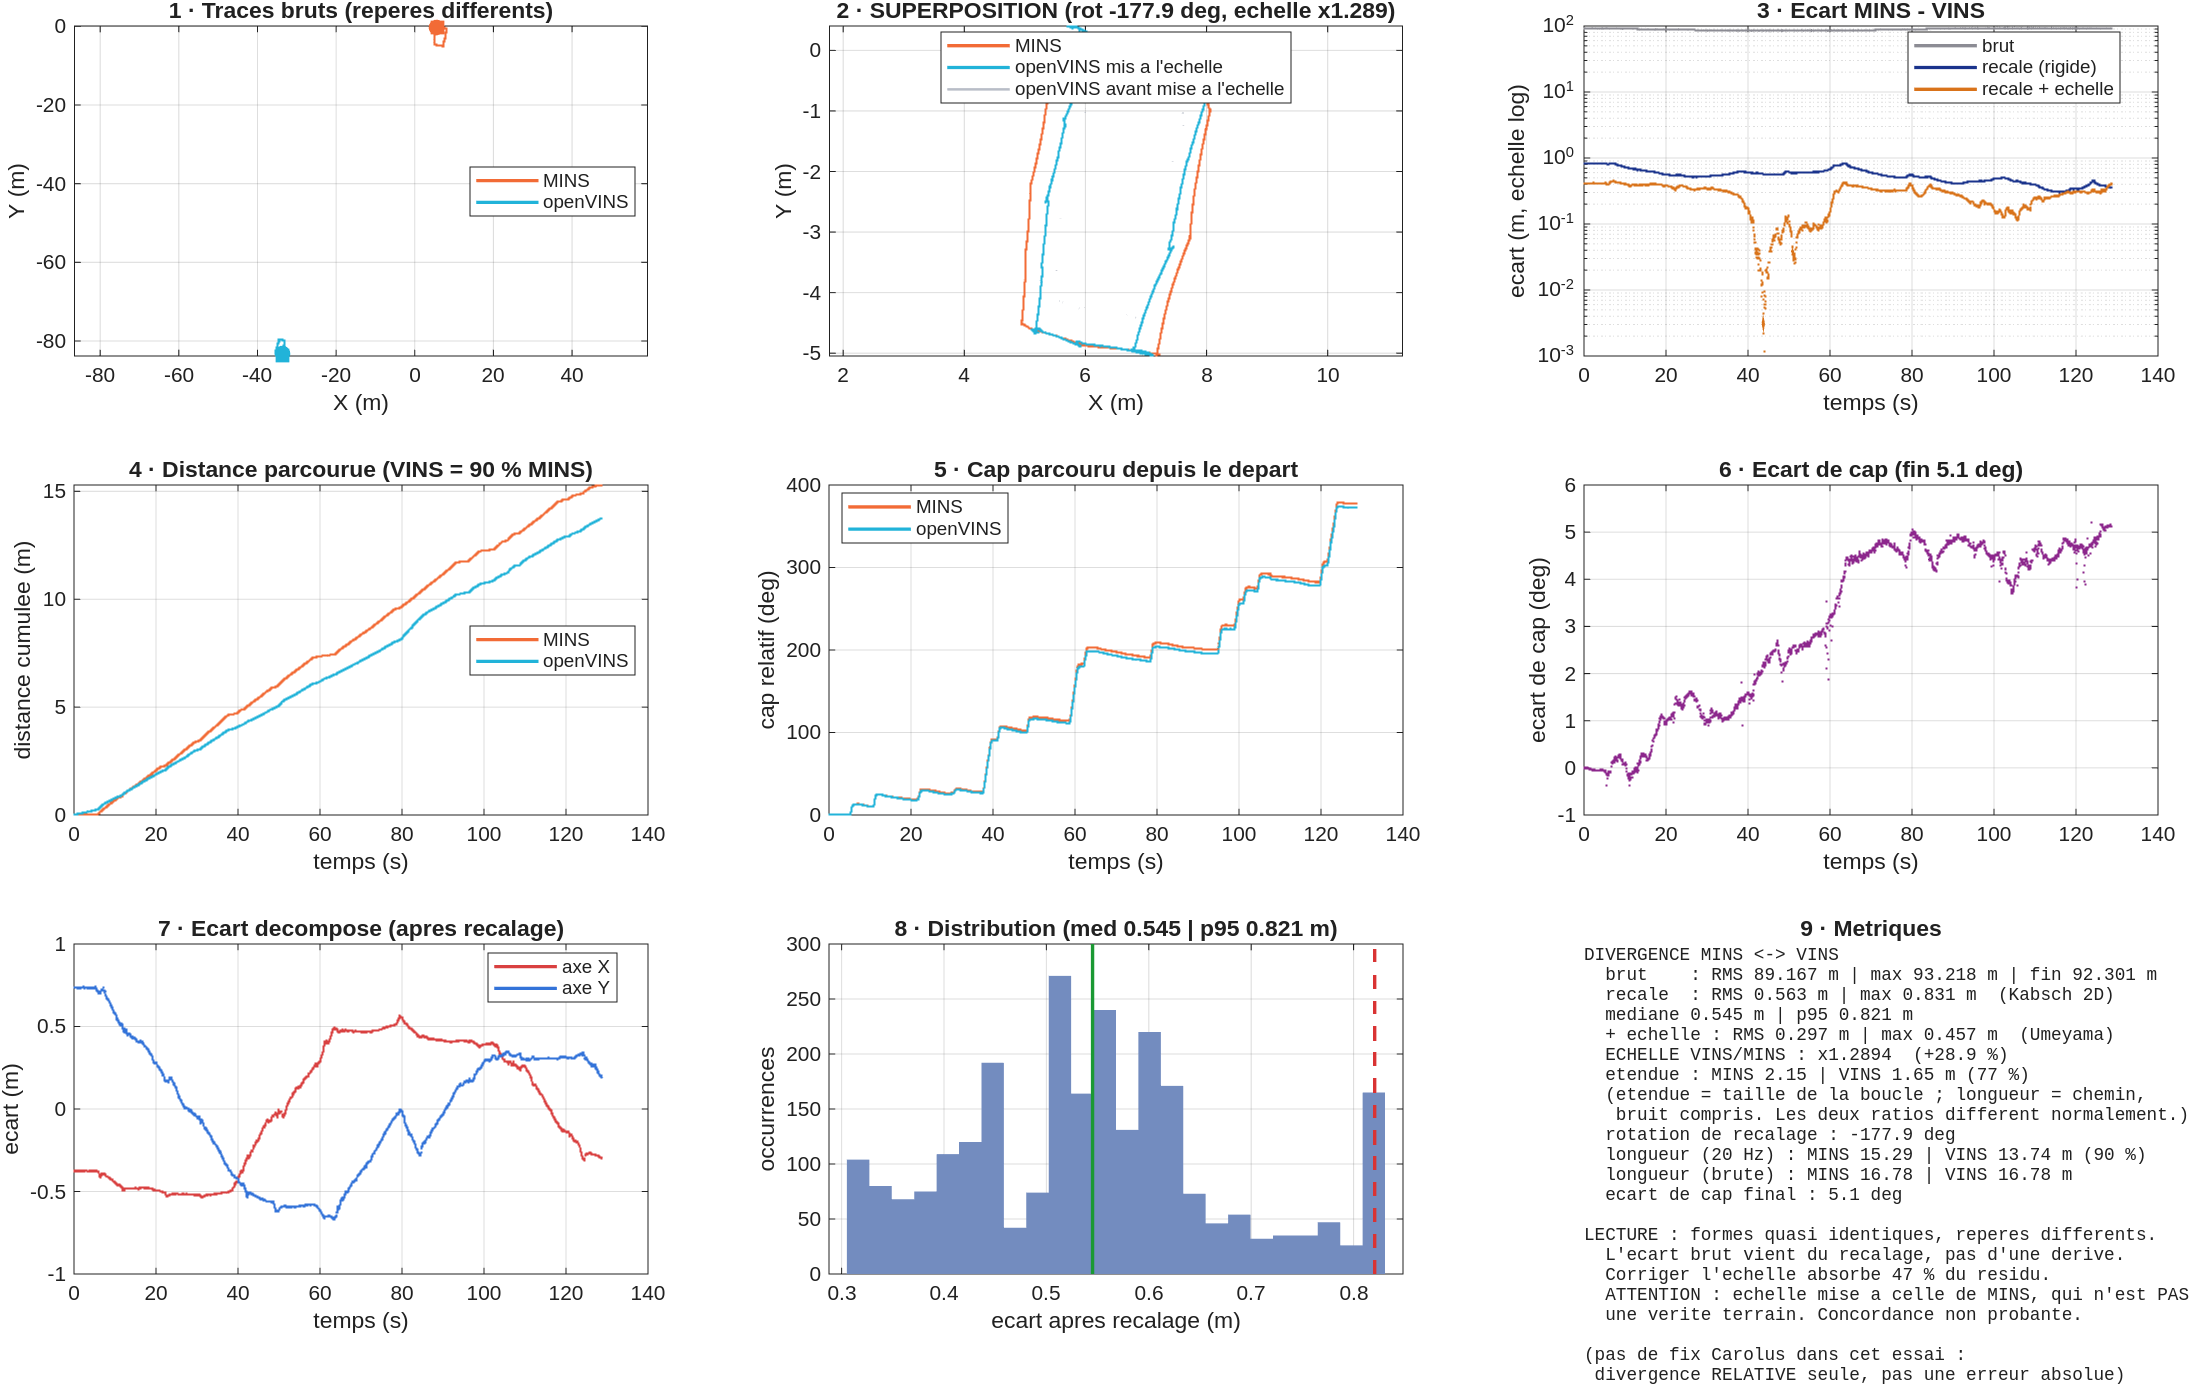
\includegraphics[width=0.84\textheight, angle=90]{figures/traj_comparison.png}%
}{%
  \fbox{\begin{minipage}[c][0.34\textheight][c]{0.9\linewidth}\centering
    \ttfamily\small [ figure placeholder ]\\[4pt]
    \normalfont\normalsize
    Placeholder for \code{plot\_trajectories.m}'s output; generated through
    the \S\ref{sec:july27pipeline} pipeline. Compiles as this box until the
    PNG exists.
  \end{minipage}}%
}
\caption{Nine-panel MINS-versus-openVINS comparison, from the first
substantive driven loop (July 29; $129$\,s, $\sim15$\,m of lab circuit, both
estimators recorded simultaneously). Read panel by panel in
\S\ref{sec:july29panels}; the mathematics behind panels~2--4 is developed in
\S\ref{sec:july29align} and \S\ref{sec:july29extent}.}
\label{fig:trajcomparison}
\label{fig:trajscale}
\label{fig:trajyaw}
\label{fig:trajresid}
\end{figure}
\fi

The pipeline was exercised end to end this session on a stationary bench
capture (MINS publishing at rest, VINS not yet initialised for want of the
jerk of \S\ref{sec:ovinit}, no beacon in view): the recorder buffered and
exported a well-formed MINS trace and the Matlab reader consumed it, but a
\emph{substantive} MINS-versus-VINS figure requires a real driven trajectory
with VINS initialised, and is logged as the first thing to capture next
(Table~\ref{tab:openitems}, item 34). Figure~\ref{fig:trajcomparison} holds
that slot.

\subsection{One-click export from the cockpit}
\label{sec:july27export}
The same data is now reachable without a terminal, and from the Trajectory
tab specifically (\code{trajectory.html}), where an operator watching the
live plot is most likely to want it. \code{leo\_backend.py} gained a
lightweight always-on trajectory recorder: it subscribes to the two raw
estimator topics and the Carolus fix, throttles each to $20$\,Hz into a
bounded ring buffer (\code{TRAJ\_MAXLEN}, $\approx 50$\,min headroom, a hard
deque bound against unbounded growth), and on an \code{export\_matlab}
command writes both a per-source CSV (the same $11$-column layout as
\code{bag\_to\_csv.py}: \code{t,x,y,z}, quaternion, and derived
\code{roll,pitch,yaw}) and a single \code{.mat} into \code{web/exports/}. The
\code{.mat} is deliberately structured for a drag-and-drop MATLAB workflow:
\code{scipy.io.savemat} writes one named struct per source
(\code{MINS}, \code{VINS}, \code{CAROLUS}), each carrying column-vector
fields \code{t,x,y,z,qx..qw,roll,pitch,yaw}, so dropping the file into MATLAB
yields three ready variables rather than an anonymous matrix. Empty sources
(e.g.\ VINS before its jerk-initialisation) are still written as empty-array
structs so the variables always exist. Because the cockpit's static server
already serves that directory, the backend reports the written filenames back
through the existing telemetry channel; the Trajectory tab watches for a new
export and \emph{immediately triggers a same-origin download} of the
\code{.mat} (a programmatic \code{<a download>} click, no popup), the
``infallible link'' the workflow needs. A companion \code{Reset} clears the
buffer to mark a fresh run. This is a convenience path layered \emph{beside}
the rosbag route of \S\ref{sec:july27pipeline}, not a replacement: the bag
remains the record for heavier off-line work (it also captures wheel odometry
and the source timeline), while the button covers the common ``drive, then
plot'' loop. Both feed the identical Matlab script, by construction.

Two smaller pieces complete the loop. \emph{Coordinate frames on the plot:}
the Trajectory canvas now subscribes to the raw \code{/tf} topic and draws
the standard RViz-style axis triads (X red, Y green) at two frames, the
\code{odom} origin and the live \code{base\_link} pose from the
\code{odom}$\rightarrow$\code{base\_link} transform. The honest caveat is
drawn into the code and the label: there is no \code{map} frame on \code{/tf}
in this architecture (the REP\,105 audit of \S\ref{sec:july24tf2}), so the
origin triad is labelled \code{odom}, the true root of the dynamic tree, not
a fabricated \code{map}. No \code{tf2\_web\_republisher} is required: the
raw topic is read directly, filtered to the one transform of interest.
\emph{Opening MATLAB directly on the plot:} the Python MATLAB Engine API is
not installed on the lab machine, but the MATLAB binary is, so on operator
request the Export button does more than write files, when the backend has
located MATLAB it \emph{launches the MATLAB desktop} on the plot
(\code{matlab -sd tools -r "plot\_trajectories('<base>.mat')"}, the GUI
\code{-r} form that leaves the desktop open, in a detached background
process), reading the freshly-written \code{.mat} directly. Two environment
details make this work from a backend that rosmon starts without a graphical
context: the launch reconstructs \code{DISPLAY} and \code{XAUTHORITY} (probed
from the running session, \code{:0} and \code{/run/user/<uid>/gdm/
Xauthority} here) so the window reaches the operator's screen, and the MATLAB
binary itself is found by probing \code{PATH} \emph{and} the known install
prefixes (the rosmon-launched backend inherits a restricted \code{PATH} that
hides \code{/usr/local/bin}). If no MATLAB is found the button falls back to
the same-origin \code{.mat} download instead. This was validated end to end
this session: the Export click wrote the \code{.mat}, the backend opened the
MATLAB desktop on the operator's display, and \code{plot\_trajectories} ran
inside it and rendered Figure~\ref{fig:trajcomparison}'s layout from the real
export. The Trajectory tab also keeps a standalone ``open in MATLAB'' button
that re-opens the last export without re-recording.

\subsection{Carolus beacon: a 6-DOF readout and a geometry-grounded LED
status}
\label{sec:july27carolus}
The Carolus channel, previously visible only as its effect on MINS, now has
two dedicated cockpit panels. The first is a direct 6-DOF readout: the
cockpit subscribes to \code{/mins/external\_ref/carolus}
(\code{geometry\_msgs/PoseStamped}, published by
\code{carolus\_vicon\_bridge.py} only while a beacon fix exists), converts
the quaternion to roll/pitch/yaw in the browser, and displays position and
orientation with a freshness watchdog that blanks the panel to ``no fix''
after $1.5$\,s of silence, honest about the fact that this fix is
intermittent by nature.

The second panel is a four-LED status cross, and its design is worth stating
precisely because it is easy to over-claim. The Carolus launch file
(\code{carolusBlobDetection.launch}) declares the beacon's four LEDs by their
metric \code{known\_points}: two on the $\pm X$ baseline
($\pm 0.0825$\,m), one on $Y$ ($0.072$\,m), one on $Z$ ($0.0555$\,m). The
detector does not label an individual blob with an axis role; what it
reports is how many of the four cluster LEDs are currently seen
(\code{detection.led\_reset.count}) and a span-derived distance. The cross
therefore drives its indicators from that count against
\emph{geometry-grounded} thresholds (the $X$ baseline needs at least the
two $\pm X$ LEDs ($\text{count}\ge 2$), $Y$ needs a third, $Z$ the full four) with a live Carolus fix (all axes actually solved by the node's PnP)
forcing all three axis dots solid, and a fourth indicator lighting on
distance acquisition. It is an observability display honestly wired to what
the pipeline computes, not a fabricated per-axis solve.

A third small panel exposes the Carolus blob-detection parameters. The
backend parses the launch file for the tunable subset (circularity,
saturation, area bounds, hue window, image threshold, distance limit) and
surfaces their current values; the cockpit shows them as editable fields
that push a \code{set\_carolus\_param} command. The honest limitation is
labelled in place: the Carolus node has no \code{dynamic\_reconfigure}, so a
change is written to the ROS parameter server and takes effect at the next
Carolus launch, not live, the panel is primarily a faithful visualiser
and a convenience for staging the next run's settings, not a live tuning
knob.

\subsection{Later the same day: from a 6-DOF readout to a robot-position and
LED-capture panel}
\label{sec:july27carolusrepurpose}
The 6-DOF panel of \S\ref{sec:july27carolus} depended on
\code{carolus\_vicon\_bridge.py} republishing
\code{/mins/external\_ref/carolus}, a topic that, on inspection later the
same day, is never actually populated: nothing publishes \code{beacon\_link}
on \code{/tf}, so the bridge has no transform to look up and the panel was
structurally always going to read ``no fix.'' Rather than patch a bridge
built on a TF frame the architecture does not produce, the panel was rebuilt
around what the vision pipeline \emph{does} reliably compute: the robot's own
local pose (\code{self.pose}, already zeroed by the LED-reset event) and the
four-LED capture status of \S\ref{sec:july27carolus} directly. AprilTag
detection was put on standby (\code{SIGSTOP} on the node: reversible,
keeps it registered on the graph without spending CPU) so operators could
focus on validating the LED-only path in isolation. The reset trigger itself
was also simplified in the same pass: it had required the LED cluster
\emph{and} the checkerboard landmark to confirm on the same tick, which
measurably never happened together in the field (the checkerboard's
rate-limited, hysteresis-held detection window rarely coincides with a fresh
LED frame), the checkerboard requirement was dropped from the reset gate
in all three call sites (manual mode, and both AUTO/LOCK paths), leaving LED
confirmation ($\ge$ \code{VISION\_CONFIRM\_FRAMES}, i.e.\ 3 consecutive valid
frames) as the sole trigger. A second, narrower fix followed a field report
of a false reset in an empty room: the LANDMARK-mode hold logic (which keeps
the last LED result ``valid'' across the mode switch to LED $\rightarrow$
LANDMARK, since the checkerboard branch would otherwise never see a
confirmed LED) had no time bound, so a stale detection could read as valid
indefinitely once the pipeline was in LANDMARK mode. A one-second bound
(\code{LED\_HOLD\_S}) was added: past it without a fresh detection, the hold
expires to \code{valid=false} rather than persisting a ghost.

\subsection{Detached MATLAB: three stacked failure modes behind ``opens then
closes,'' and a rendering bug hiding in the pipeline itself}
\label{sec:july27matlabfix}
The MATLAB launch of \S\ref{sec:july27export} was validated again later the
same day against a harder condition, the watchdog's automatic stack
restarts firing while a MATLAB session was open, whose root cause was
only identified two days later and is documented in
\S\ref{ap:repro-watchdog}, and failed: the window closed within seconds of a restart, and separately
even without one. Three independent causes were isolated, each confirmed by
a controlled before/after test rather than inferred from a single
observation.

First, \code{start\_new\_session=True} (a \code{setsid} equivalent) protects
the child from an \code{os.killpg()} targeting \code{leo\_backend.py}'s own
process group, exactly how \code{roslaunch} tears down a node on
restart, but a watchdog-triggered restart still killed MATLAB regardless.
The fix is a genuine double-fork: \code{tools/matlab\_daemon.sh} backgrounds
the launch (\verb|cmd & disown|) and exits immediately without waiting,
orphaning the job so the kernel reparents it to \code{init} (observed here as
\code{systemd --user}) rather than to \code{leo\_backend.py}, structurally
outside any cleanup that walks the backend's process tree, by group or by
PPID. Verified directly: a test process launched this way kept a PPID of
\code{1774} (\code{systemd --user}) after the wrapper exited, and a real
MATLAB session launched through the daemon script survived two genuine
watchdog-triggered stack restarts inside one continuous 280-second window, though a later false positive from the same test methodology (PID reuse
under heavy process churn, caught by cross-checking \code{/proc/<pid>/cmdline}
rather than \code{kill -0} alone) is recorded here as a caution for repeating
this class of test.

Second, and unrelated to any restart: MATLAB launched via \code{-r} exits
cleanly (exit code \texttt{0}, no crash, no error) as soon as the given
command finishes, if its \code{stdin} is not a real terminal, which a
process started by \code{rosmon} never has. The documented behaviour (``\code{-r}
keeps the desktop open'') holds only with an interactive terminal attached.
The fix allocates a real pty for the launch, via the standard \code{script}
utility (\verb|script -qefc "$cmdstr" "$log"|) inside the same daemon script,
combined with the double-fork above. One accepted side effect: with a real
pty present, MATLAB routes its banner and \code{fprintf} output to the GUI
console rather than mirroring it to the pty, so \code{matlab\_launch.log}
now records only \code{script}'s own start/exit trailer (including the exit
signal, e.g.\ \texttt{137} for a kill) rather than the full transcript,
diagnostic depth traded for the fix that actually mattered.

Third, and the one that had been masking the first two in testing: even with
both fixes applied, a real export-triggered launch still closed within
seconds. \code{leo\_backend.py} runs with no desktop session at all: not
only no \code{DISPLAY}, but no \code{XDG\_RUNTIME\_DIR} and no
\code{DBUS\_SESSION\_BUS\_ADDRESS} either, confirmed empty in
\code{/proc/<pid>/environ} where a normal login session always has them,
because the stack is (re)launched by the watchdog's cron job rather than a
user session and inherits cron's own cgroup
(\code{system.slice/cron.service}). A controlled A/B test made this decisive:
the identical launch command, from an otherwise-identical minimal
environment, died in under five seconds without those two variables and ran
for over a minute cleanly with them added. \code{\_gui\_env()} now
reconstructs both from the standard \code{/run/user/<uid>} paths, alongside
\code{DISPLAY}/\code{XAUTHORITY}, each only when the process does not already
have a valid one and the expected path exists on disk. The complete fix (double-fork, pty, and the session variables together) was confirmed
against the real cockpit button: a PID verified alive for 105 continuous
seconds via \code{/proc/<pid>/cmdline}, spanning one genuine automatic
watchdog restart mid-window.

A fourth, unrelated defect surfaced only by looking directly at a rendered
figure rather than confirming a PNG merely existed: \code{plot\_trajectories.m}
had been silently mis-rendering every trajectory line it drew, all
session, a \code{plot(x, y, '-', \ldots)} call with several hundred
points rasterises only short fragments near locally steep sections and drops
near-flat sections entirely, reproduced independently of renderer choice
(\code{opengl}/\code{painters}/\code{-softwareopengl}), export function
(\code{saveas}/\code{print}/\code{exportgraphics}), \code{LineJoin}, and
\code{GraphicsSmoothing}. Adding a marker to the same line
(\verb|'Marker','.','MarkerSize',3|) renders correctly, which is the applied
fix in both \code{plot\_trajectories.m} and the new
\code{compare\_tests.m} of \S\ref{sec:july27twotest}, a workaround, not a
root-caused explanation, but confirmed to fully restore every trajectory
figure this pipeline produces. Every comparison PNG generated before this fix
is visually wrong and should be regenerated, not just re-copied.

\subsection{Carolus at working distance: the D455 colour stream, re-enabled
under an explicit CPU budget}
\label{sec:july27color}
The 6-DOF beacon pose of \S\ref{sec:july27carolus} needs \code{carolus\_astrobee}
to see actual colour frames, and the D455's colour stream had been disabled
since July~6 for a documented reason recorded directly in
\code{/etc/ros/robot.launch}: at its default profile the colour stream alone
saturated the Pi's CPU badly enough to starve the rosserial link and desync
the IMU. That risk materialised again, independently, later in this same
session (an unrelated colour-camera re-enable attempt drove the Pi to
sustained thermal throttling and a total, if temporary, loss of drivable
control: resolved by disabling colour again and cycling the stack). Given
an explicit, informed decision to accept the residual thermal risk (a fan is
the planned permanent fix) and re-enable the channel for beacon work, two
changes were made together rather than repeating the earlier attempt as-is.
First, the colour stream is now launched with the same explicit
$640{\times}480@15\,$Hz budget already used for infra/depth
(\code{color\_width}/\code{color\_height}/\code{color\_fps} were previously
unset, silently falling back to a much heavier default profile:
plausibly the actual reason the July-6 measurement was as bad as it was).
Second, \code{carolus\_astrobee} itself has no internal frame-rate
parameter, it processes every frame its subscribed topic delivers, so
its CPU cost is decoupled from the camera's native rate with a standard
\code{topic\_tools/throttle} node inserted ahead of it
(\code{carolus\_detect.launch}, default $4\,$Hz, configurable by launch
argument), no source changes required. Measured after both changes: Pi
temperature settled from an already-elevated $86\text{--}87\,^{\circ}\mathrm{C}$
baseline down to $\approx 84\,^{\circ}\mathrm{C}$, \code{realsense2\_camera\_manager}
dropped from the $148\text{--}187\,\%$ CPU observed in the earlier incident
to $\approx 30\text{--}65\,\%$, and \code{carolus\_astrobee} plus the
throttle node together stayed under $1\,\%$ CPU at idle. The permanent fix
remains physical (active cooling); this is a working mitigation, not a
substitute for it.

\subsection{A two-test protocol: Test 1 (MINS) versus Test 2 (openVINS), and
the closing comparison this campaign has been building toward}
\label{sec:july27twotest}
Every earlier subsection in this session's work is plumbing (a pipeline,
an export button, a beacon panel, a thermal budget) built toward a single
outstanding measurement (Table~\ref{tab:openitems}, item 34): a real driven
loop of the lab, compared honestly between MINS and openVINS. The Trajectory
tab now has the protocol to produce it directly. A two-way selector
(\code{TEST 1} / \code{TEST 2}) labels the currently-buffered run; it changes
nothing about \emph{what} is recorded (both estimators are always captured
together, which is the entire point of the comparison): it only relabels
where the Export button writes its files, from the generic timestamped name
to a predictable \code{<label>\_<source>.csv} / \code{<label>.mat}
(e.g.\ \code{test1\_mins.csv}, \code{test2\_vins.csv}). The protocol this
enables: select \emph{Test 1}, drive the lab loop under active MINS,
export; switch to \emph{Test 2}, reset, drive the same loop under active
VINS, export. Two predictably-named files, one per estimator, each on its
own physical run of the same loop.

A new script, \code{tools/compare\_tests.m}, consumes exactly that pair. It
is deliberately \emph{not} the Kabsch-aligned divergence of
Eq.~\ref{eq:kabsch}, that comparison is only meaningful when both
estimators observe the \emph{same} motion at the \emph{same} instants, which
two separate drives are not. Two independent runs of a loop admit a
different, equally honest pair of readings instead: path length (a
coarse cross-check that both runs covered a comparable distance) and
\emph{loop-closure error}, the distance between each trajectory's first
and last point. A lab circuit returns close to its start; the residual gap
after a full loop is a direct, if approximate, proxy for the drift
accumulated by that estimator over that run, in the continued absence of
absolute ground truth. Heading drift (final yaw minus initial yaw, wrapped)
is reported alongside it. The script was verified against synthetic
circular trajectories with injected drift before being trusted on real data,
and inherits the marker-line fix of \S\ref{sec:july27matlabfix}.

\begin{figure}[htbp]
\centering
\IfFileExists{figures/test_comparison.png}{%
  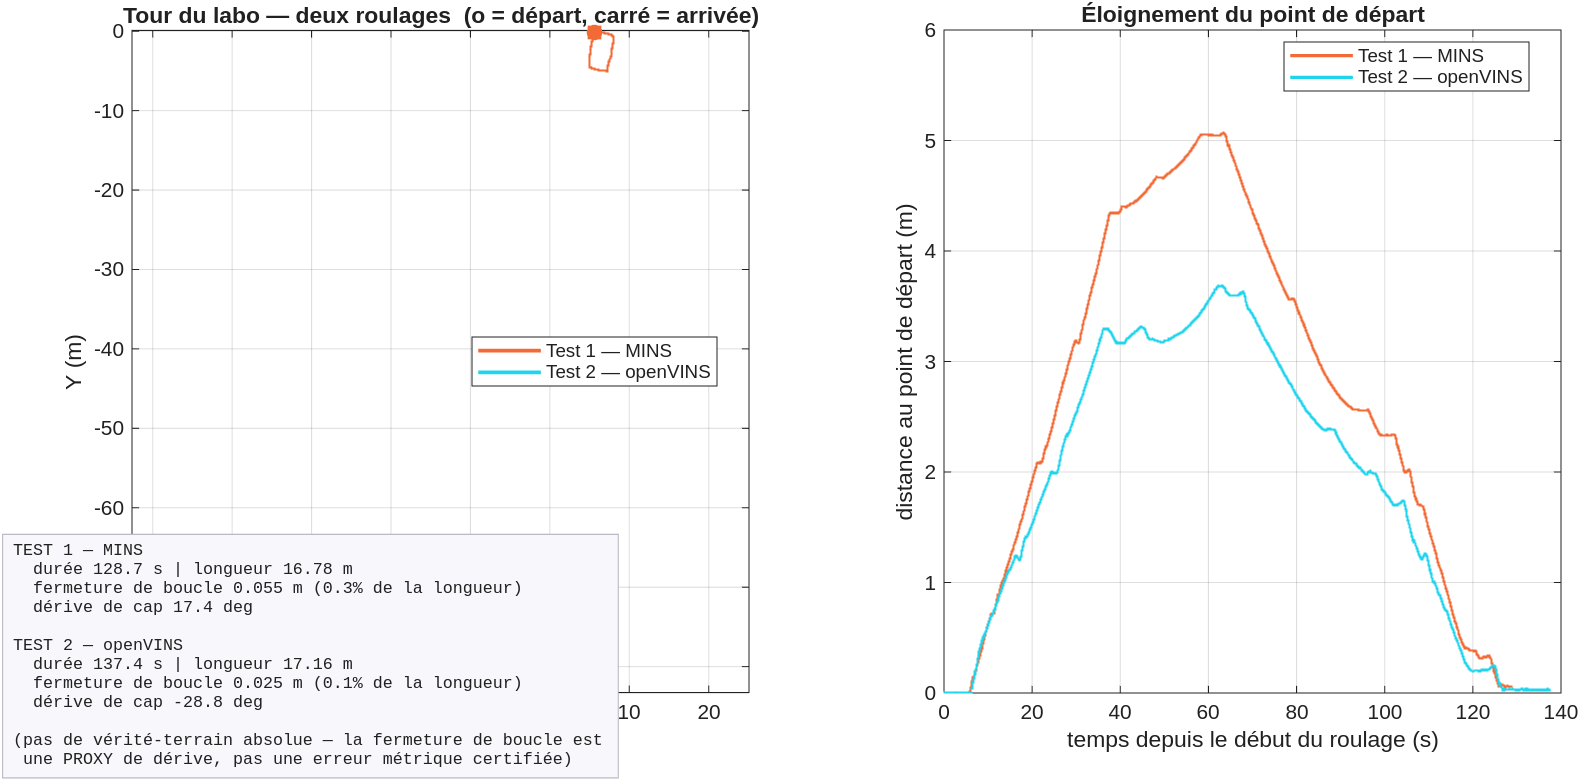
\includegraphics[width=0.92\linewidth]{figures/test_comparison.png}%
}{%
  \fbox{\begin{minipage}[c][0.34\textheight][c]{0.9\linewidth}\centering
    \ttfamily\small
    [ figure placeholder ]\\[4pt]
    \normalfont\normalsize
    Placeholder for \code{compare\_tests.m}'s output. Generated by: cockpit
    Trajectory tab, \emph{Test 1} $\rightarrow$ drive the loop
    $\rightarrow$ Export; \emph{Test 2} $\rightarrow$ reset $\rightarrow$
    drive the same loop $\rightarrow$ Export; then
    \code{compare\_tests()}, which reads \code{web/exports/test1.mat} and
    \code{test2.mat} and saves \code{test\_comparison.png}/\code{.pdf}
    directly into this directory. Compiles as this box until the PNG
    exists.
  \end{minipage}}%
}
\caption{Test 1 (MINS, orange) versus Test 2 (openVINS, cyan): two
independent drives of the same lab loop. Left: planar trajectories
($\circ$ start, $\square$ end). Right: each run's distance from its own
start point over time, a loop that closes returns this curve to zero by
the end; the residual is the loop-closure error reported alongside path
length and heading drift.}
\label{fig:testcomparison}
\end{figure}

\paragraph{Reading the result.}
This subsection was originally drafted ahead of the two drives it analyses,
scaffolded with the exact numbers and judgement calls the closing analysis
would need, so that filling it in would be a matter of driving the loop
twice and transcribing the script's own printed output rather than
re-deriving the comparison from scratch. Both drives now exist
(\code{test1\_20260729\_145637}, \code{test2\_20260729\_145417}): what
follows is that transcription, not a template.

\begin{itemize}
\item \textbf{Path length.} MINS: $16.78$ m. openVINS:
  $17.16$ m. If the two differ by more than a few percent, that is
  itself informative: it means the two runs did not cover quite the same
  physical path (operator steering variation between drives), and the
  loop-closure numbers below should be read as slightly less directly
  comparable, not as a pure estimator-quality contrast.
\item \textbf{Loop-closure error.} MINS: $0.055$ m
  ($0.3$\,\% of path length). openVINS:
  $0.025$ m ($0.1$\,\%). This is the headline
  number: the estimator with the smaller closure error drifted less over a
  comparable loop. State which one, by how much, and whether the gap is
  large relative to the platform's demonstrated static-drift floor
  (Protocol T1.1, \S\ref{sec:t11}), a closure error near that floor says
  the estimator tracked the loop about as well as it tracks standing still;
  one well above it says the loop itself (turns, speed changes, feature
  density around the room) is where the drift is actually accumulating.
\item \textbf{Heading drift.} MINS: $+17.4$$^\circ$. openVINS:
  $-28.8$$^\circ$. Large heading drift with small loop-closure
  error is possible and worth flagging explicitly if seen: it means
  position happened to be self-correcting around the loop shape while
  orientation still wandered, which loop-closure error alone would not
  reveal.
\item \textbf{Qualitative trajectory shape.} Both runs close visibly as
  loops in Figure~\ref{fig:testcomparison}'s left panel, with no kink or
  gross corner-cutting in either; the path lengths differ by $2.3\%$
  ($16.78$ against $17.16$\,m), which is within the operator-steering
  variation this subsection anticipated and small enough that the closure
  figures below stay comparable. The difference between the two estimators
  on this loop is therefore not visible in the trajectory shape: it is
  visible only in the heading channel, which is precisely why the numeric
  readings below matter more than the picture.
\item \textbf{Conditions during each drive.} Both drives were made
  indoors on the lab carpet under fixed ceiling lighting, on mains power
  ($12.0$\,V, $78\%$), within three minutes of one another
  (\code{test1\_20260729\_145637}, \code{test2\_20260729\_145417}). No
  Carolus fix was in view during either run, so the ground-truth-anchored
  error of \S\ref{sec:july27pipeline} could not be computed and only mutual
  divergence is available. The Pi was thermally throttled throughout, at
  $86\,^\circ$C and a capped $600$\,MHz: the condition characterised in
  \S\ref{sec:july29calib} as the origin of the gaps in the IMU stream, and a
  standing caveat on both runs. Critically, and unlike every earlier attempt
  in this campaign, \emph{no watchdog restart interrupted either drive}: the
  cron \code{PATH} defect that had been destroying the stack every
  $\sim2$\,min was diagnosed and fixed earlier the same day, and the
  watchdog log records zero automatic restarts across July 29. Every
  estimator measurement taken before that fix was made on a stack being torn
  down mid-run, which is why this pair is the first that can be read at
  face value.

  For any future repetition of this protocol, the conditions worth
  recording alongside the data are the floor surface and the ambient
  lighting, whether the beacon was in view for either run (a Carolus fix
  during Test 1 or Test 2 would let \S\ref{sec:july27pipeline}'s
  ground-truth-anchored error be computed too, not just mutual divergence),
  Pi temperature/throttling state (\S\ref{sec:july27color}), and whether the
  watchdog restarted the stack mid-drive (the cron watchdog's automatic
  full-stack restarts remain an open, unresolved instability at the time of
  writing, worth recording explicitly if one interrupted either test,
  since a mid-drive backend restart clears the trajectory buffer and would
  truncate that run's export).
\item \textbf{Verdict.} On loop-closure error
  alone openVINS is the better performer here, by a factor of $2.2$
  ($0.025$ against $0.055$\,m), and both figures sit within the same order of
  magnitude as the platform's static planar floor of $\sim8$\,mm in $X$ and
  $\sim1$\,mm in $Y$ (Table~\ref{tab:t11}), that is, on this loop neither
  estimator accumulated much more position error while driving than it does
  standing still, which is a stronger result for both than this campaign's
  earlier sessions would have predicted. The heading channel reverses the
  ranking: openVINS drifted $-28.8^\circ$ against MINS's $+17.4^\circ$,
  $65\%$ worse in magnitude and in the opposite sense. This is exactly the
  combination flagged as worth reporting above, small closure error with
  large heading drift, and it is the expected signature of a
  loosely-constrained orientation channel whose position happens to be
  self-correcting around a closed loop: a heading error accumulated on one
  leg is partly undone on the return leg, so the loop closes while the
  orientation estimate has genuinely wandered. It also matches the
  independent evidence of Figure~\ref{fig:trajcomparison} panel~6, where the
  MINS--openVINS heading disagreement grows to $\sim5^\circ$ within a single
  simultaneous run. The two readings agree, from different data, that
  orientation is where openVINS is weakest on this platform.

  The honest verdict is therefore split rather than clean, and it is one data
  point. For unattended patrol, where heading error compounds into
  navigation error over minutes, MINS remains the safer default on this
  evidence, notwithstanding its larger closure error, and it is also the only
  estimator whose scale has been checked against a tape measure
  ($-4\%$, \S\ref{sec:july29calib}). That is consistent with the
  architectural expectation of \S\ref{sec:whymsckf} only in part: the
  tightly-coupled wheel constraint does appear to be anchoring orientation,
  but it did not deliver the better position closure on this loop, which the
  architectural argument alone would have predicted. Turning this into a
  conclusion needs at least two further loops on different days and under
  different lighting, run after the thermal throttling is resolved, and with
  a Carolus fix in view so that absolute error, not merely mutual
  divergence, can be computed. On
  these specific conditions, which estimator is the better default for
  unattended patrol, and does that verdict agree with or contradict the
  architectural expectation set in \S\ref{sec:whymsckf} (MSCKF
  tightly-coupled versus a loosely-coupled alternative)? A single loop is
  one data point, not a validated conclusion, state it as such, and note
  what a second and third loop (ideally on different days, different
  lighting) would need to show to turn this into one.
\end{itemize}

%=============================================================================
\section{Field session, July 28: a starved serial link, a single boolean
worth four orders of magnitude, and an accelerometer out of spec}
\label{sec:july28}

Three findings were made on this day, and their interest lies less in each
one than in how they interlock. A scheduling defect was corrupting the
inertial stream; an out-of-spec sensor was making the corruption
catastrophic rather than merely untidy; and a single configuration flag was
the only thing standing between the two and a divergence of forty kilometres.
Each was found while investigating a different symptom, which is the usual
way, and none is intelligible without the others.

\subsection{The serial link was starving, not failing}
\label{sec:uartrtprio}

The presenting symptom had been recurring for a week and had twice been
attributed to hardware: \code{wrong checksum for topic id and msg} in the
thousands, \code{/firmware/wheel\_states} collapsing to $1$\,Hz, and
\code{firmware\_message\_converter} left with no wheel data to convert. The
CORE2 board and its cabling had been the standing suspects.

The measurement that settled it was the kernel's own overrun counter, which
is specific in a way checksum errors are not. A checksum error says a frame
arrived corrupted; an overrun says the receiver discarded a byte because
nobody read the FIFO in time. The counter stood at $137\,000$ and was
advancing at $63$ per $10$\,s. That is not a cabling fault, and no amount of
physical inspection would ever have found it: the bytes were arriving
correctly and the operating system was failing to collect them.

Two causes were acting together. The Pi was thermally capped at $600$\,MHz,
so every code path took two and a half times longer than at nominal clock,
and \code{serial\_node} ran at ordinary scheduling priority, so it waited
behind every other runnable task on a machine already oversubscribed.
\S\ref{sec:july30thermal} develops the deadline model that makes this
quantitative; the operational summary is that the port must be serviced
within $1.28$\,ms and neither condition allowed it.

The fix has two halves and needs both:
\begin{lstlisting}[language=bash]
# 1. real-time priority for the serial node
chrt -f 25 <serial_node pid>
# 2. permission for leo.service to grant it (drop-in)
[Service]
LimitRTPRIO=50
\end{lstlisting}
Applying the first without the second does not merely fail to help: the node
refuses to start, because a service whose \code{RLIMIT\_RTPRIO} is zero
cannot raise its own scheduling class. This is worth stating plainly because
the failure presents as ``the fix broke the serial node'', which invites
reverting the very change that was correct.

The result was immediate and large. Wheel odometry went from $1$\,Hz to
$19$\,Hz, and the checksum storm stopped. A secondary discovery followed from
looking at the process table with fresh attention: an orphaned
\code{rosbridge\_server} was running \emph{on the robot}, consuming $96\,\%$
of a core to serve nothing, on a machine whose scarcity of CPU was the entire
problem. It had no business being there and was terminated.

\subsection{One boolean, and a divergence of $41\,824$ metres}
\label{sec:july28zupt}

With the inertial stream finally clean, openVINS was expected to behave. It
did not. A stationary run produced a final position estimate $41\,824$\,m
from the origin, which is to say that a rover parked on a carpet had
concluded it was somewhere past the edge of the county.

A divergence of that magnitude is not a tuning problem and should not be
treated as one. It is large enough to identify its own mechanism, because
only a double integration can produce it. The culprit was a single line in
\code{estimator\_config.yaml}:
\begin{lstlisting}[language=bash]
try_zupt: false      # -> 41 824 m
try_zupt: true       # ->      0.002 m
\end{lstlisting}
Four orders of magnitude, and then four more, from one boolean.

\paragraph{Why it matters so much, and only to this estimator.}
Zero-velocity updates exist because a stationary visual-inertial platform is
an observability hole. When the rover does not move, the camera contributes
no parallax and therefore no scale information, and the accelerometer sees
only gravity plus its own errors. Writing the specific force as
\begin{equation}
\mathbf{a}_m = K_a\,(\mathbf{a} - \mathbf{g}) + \mathbf{b}_a
             + \boldsymbol{\eta}_a ,
\label{eq:july28specific}
\end{equation}
at rest $\mathbf{a} = \mathbf{0}$, so anything the filter cannot attribute to
gravity is integrated twice into position:
\begin{equation}
\Delta p(t) \;=\; \tfrac{1}{2}\,\lVert \mathbf{r} \rVert\,t^{2},
\qquad
\mathbf{r} = (K_a - I)\,\mathbf{g} + \mathbf{b}_a ,
\label{eq:july28doubleint}
\end{equation}
with no measurement anywhere in the filter opposing it. A ZUPT supplies
exactly the missing constraint, asserting $\mathbf{v} = \mathbf{0}$ and
thereby making the residual $\mathbf{r}$ observable instead of free.

MINS, running on the same data on the same day, did not diverge and does not
need the flag. The reason is structural rather than a matter of quality:
MINS consumes wheel odometry, and a wheel encoder reporting zero rotation is
itself a zero-velocity measurement, delivered continuously and without any
detection logic. The estimator that fuses the wheels gets its ZUPT for free;
the camera-and-IMU estimator has to be told to look for it. This is the
sharpest illustration in the campaign of what the extra sensor actually buys.

\begin{trapbox}{Testing a configuration from the wrong directory}
An earlier attempt to validate this had produced a false negative. The
configuration was edited and tested from a copy under \code{/tmp}, while the
running node loaded its own file from the workspace. The test exercised a
file nobody was reading. Always confirm which path the live node opened, with
\code{rosparam get} or by reading the node's startup log, before concluding
that a configuration change has no effect.
\end{trapbox}

\noindent Two further defects were cleared the same evening, both recorded in
\S\ref{ap:repro-config}: a mutex crash firing $1324$ times, once every
$46$\,s, whose root cause split into an OpenCV \code{FileStorage} parser
aborting on an over-long inline YAML comment at startup, and OpenCV's own
thread pool at runtime, resolved by pinning
\code{num\_opencv\_threads: 1}.

\subsection{Why the divergence was that large: an accelerometer $10.6\,\%$
out of spec}
\label{sec:july28accel}

Equation~\ref{eq:july28doubleint} says the divergence rate is set by the
residual $\mathbf{r}$, so the natural question is how large $\mathbf{r}$
actually was. The stationary characterisation of \S\ref{sec:imucalib}
answers it: the accelerometer reported $8.7525$\,m/s$^2$ against a true local
gravity of $9.790$\,m/s$^2$ at latitude $28^\circ$, an error of $-10.6\,\%$
lying in the raw sensor rather than anywhere in the processing chain. The
residual is therefore
\begin{equation}
\lVert \mathbf{r} \rVert \;=\; 9.790 - 8.7525 \;=\; 1.06\ \text{m/s}^2 .
\label{eq:july28residual}
\end{equation}

Substituting into Eq.~\ref{eq:july28doubleint} gives $\Delta p \approx
1900$\,m after one minute, and the observed $41\,824$\,m corresponds to
\begin{equation}
t \;=\; \sqrt{\frac{2 \times 41\,824}{1.06}} \;=\; 281\ \text{s}
  \;\approx\; 4.7\ \text{minutes},
\label{eq:july28consistency}
\end{equation}
which is the right order for the run in question. The agreement is a
consistency check rather than a proof, since the run duration was not
recorded to the second, but it closes the argument: the three findings of
this day are one causal chain. The scheduling defect corrupted the inertial
stream, the out-of-spec accelerometer set the divergence rate once the
stream was clean, and the ZUPT flag was the only mechanism capable of
observing and cancelling it.

\paragraph{What this means for every comparison in this chapter.}
An accelerometer $10.6\,\%$ out of spec is not a nuisance to be tuned around.
Until it is corrected in the sensor or compensated in the model, any
MINS-versus-openVINS comparison measures, in part, which estimator better
tolerates a known-bad accelerometer. MINS survives it because the wheels
anchor the solution; openVINS survives it only because ZUPT is enabled. That
is a real and reportable difference in robustness, and it is emphatically not
the same statement as one estimator being more accurate than the other. The
distinction is recorded in Table~\ref{tab:openitems} so that no later reader
mistakes the one for the other.

\section{Field session, July 29: trajectory alignment as a measurement, and
the first ground-truth calibration}
\label{sec:july29}
The comparison pipeline of \S\ref{sec:july27pipeline} produced its first
substantive driven loop on July 29: $129$\,s of manual lab circuit,
$\sim15$\,m of path, both estimators running and recorded together. The
figure it produced (Fig.~\ref{fig:trajcomparison}) is the deliverable this
campaign has been building toward since item~34 was opened. Reading it
correctly, however, turned out to require more care than plotting it, and
this section develops the mathematics that the plot only summarises. Two
results are established: an exact decomposition that separates a
\emph{scale} disagreement from a \emph{shape} disagreement
(\S\ref{sec:july29align}), and a noise model that explains why two perfectly
reasonable definitions of ``how far did it travel'' give different answers,
and why one of them must never be compared across sampling rates
(\S\ref{sec:july29extent}). A third subsection reports the first
measurements on this platform made against physical ground truth rather than
against another estimator (\S\ref{sec:july29calib}).

\subsection{Reading the panels}
\label{sec:july29panels}
Each panel answers a question the others cannot, and several of the
conclusions in this section are visible only by reading two panels
\emph{against} each other, which is why they are grouped in pairs across
Figs.~\ref{fig:trajcomparison}--\ref{fig:trajresid} rather than presented as
one combined plate. (\code{plot\_trajectories.m} still produces the combined
$3\times3$ plate for on-screen use; at page width its individual panels fall
below $5$\,cm and become unreadable, so the report uses the separately
exported $200$\,dpi versions instead.)

\begin{description}\itemsep2pt
\item[\textbf{1: raw traces.}] The two estimates as served, sharing no
  frame. They sit $90$\,m apart and look unrelated. Included deliberately:
  this is the honest starting point, and it measures nothing but the
  arbitrariness of two independent origins.
\item[\textbf{2: superposition.}] The same pair after the similarity
  alignment of Eq.~\ref{eq:umeyama}, with openVINS \emph{before} rescaling
  retained in pale grey so the magnitude of the correction stays visible.
  This is the only view in which the eye can judge whether the two
  estimators describe the same motion.
\item[\textbf{3: separation versus time.}] Raw, rigid-aligned and
  scale-corrected, on a logarithmic axis, without which the $\sim0.5$\,m
  aligned curves collapse onto the axis beneath the $90$\,m raw one. The
  scale-corrected trace dips to $10^{-3}$\,m near $t\approx45$\,s.
\item[\textbf{4: cumulative path length.}] Two distinct slopes, exposing
  a scale disagreement that panel~2 is constructed to hide. Panels~2 and~4
  must therefore be read together, never separately.
\item[\textbf{5: heading accumulated from the start.}] Both estimators,
  relative to their own initial heading, so the staircase of successive
  turns can be compared directly.
\item[\textbf{6: heading difference.}] The angular disagreement in
  isolation: flat until $t\approx40$\,s, then a rise to $\sim5^\circ$
  between $t\approx40$ and $t\approx70$\,s, after which it plateaus. A
  drift confined to one phase of the drive, not a uniform bias.
\item[\textbf{7: residual decomposed onto $X$ and $Y$.}] Post-alignment,
  and the decomposition matters: a residual concentrated on one axis is a
  directional bias, which is corrected differently from isotropic noise.
  Here both components are smooth $\pm0.5$\,m excursions, a slowly
  varying disagreement, not sample-to-sample scatter.
\item[\textbf{8: residual distribution.}] Median and $95$th percentile
  marked. Reported because the mean of a divergence is a poor summary when
  the damage lives in the tail, a lesson this campaign learned the hard way.
\item[\textbf{9: metric summary.}] Every figure quoted in this section,
  plus the caveat the script prints whenever the fitted scale departs from
  unity by more than $3\%$: that the scale was fitted to MINS, and that MINS
  is not ground truth.
\end{description}

\subsection{Rigid versus similarity alignment: two residuals, and the exact
identity that separates them}
\label{sec:july29align}
Neither estimator is expressed in a frame the other shares. MINS and
openVINS each initialise their own origin and their own initial heading, so
the raw separation between them ($89.2$\,m RMS on this run) measures
nothing about either estimator's quality. It measures only that two
arbitrary frames are arbitrary. Panel~1 of Fig.~\ref{fig:trajcomparison}
shows exactly this and is included deliberately: the two traces sit $90$\,m
apart and look unrelated, which is the honest starting point.

The rigid alignment of Eq.~\ref{eq:kabsch} removes the frame difference and
leaves a residual that measures shape agreement. Written with the estimator
roles explicit, let $\{\mathbf{p}_k\}_{k=1}^{n}$ be the openVINS positions
and $\{\mathbf{q}_k\}_{k=1}^{n}$ the MINS positions, both resampled onto the
common $20$\,Hz base so that index $k$ denotes the same instant in both.
Introducing the centroids and the centred coordinates
\begin{equation}
\bar{\mathbf{p}}=\frac1n\sum_k \mathbf{p}_k,\qquad
\tilde{\mathbf{p}}_k=\mathbf{p}_k-\bar{\mathbf{p}},\qquad
\sigma_p^{2}=\frac1n\sum_k\lVert\tilde{\mathbf{p}}_k\rVert^{2},
\label{eq:centroids}
\end{equation}
and identically for $\mathbf{q}$, the quantity $\sigma_p$ is the RMS radius
of the openVINS trace about its own centroid. It is referred to below as the
\emph{spatial extent}, and it will matter a great deal in
\S\ref{sec:july29extent}.

The similarity alignment admits a scale factor alongside the rotation and
translation:
\begin{equation}
(s^{\star},R^{\star},\mathbf{t}^{\star})=
\operatorname*{arg\,min}_{s>0,\;R\in SO(2),\;\mathbf{t}\in\mathbb{R}^{2}}
\;\frac1n\sum_{k=1}^{n}
\bigl\lVert \mathbf{q}_k-(s\,R\,\mathbf{p}_k+\mathbf{t})\bigr\rVert^{2}.
\label{eq:umeyama}
\end{equation}
Its closed-form minimiser is Umeyama's \cite{umeyama1991}: form the
cross-covariance and its singular value decomposition,
\begin{equation}
\Sigma=\frac1n\sum_k\tilde{\mathbf{q}}_k\tilde{\mathbf{p}}_k^{\top}
      = U\,D\,V^{\top},\qquad D=\operatorname{diag}(d_1,d_2),\;d_1\ge d_2\ge 0,
\label{eq:crosscov}
\end{equation}
and let $S=I$ when $\det\Sigma\ge 0$ and $S=\operatorname{diag}(1,-1)$
otherwise, the correction that forbids the minimiser from ``fitting'' a
reflection, which would silently mirror one trajectory onto the other and
report a spuriously small residual. Then
\begin{equation}
R^{\star}=U S V^{\top},\qquad
s^{\star}=\frac{\operatorname{tr}(DS)}{\sigma_p^{2}},\qquad
\mathbf{t}^{\star}=\bar{\mathbf{q}}-s^{\star}R^{\star}\bar{\mathbf{p}} .
\label{eq:umeyamasol}
\end{equation}
Setting $s\equiv1$ in Eq.~\ref{eq:umeyama} recovers the rigid problem of
Eq.~\ref{eq:kabsch}, whose minimiser is the same $R^{\star}$ with
$\mathbf{t}=\bar{\mathbf{q}}-R^{\star}\bar{\mathbf{p}}$.

\begin{figure}[htbp]
\centering
\begin{tikzpicture}[scale=0.95, every node/.style={font=\small}]
  % ---- stage 1 : raw, two unrelated frames
  \begin{scope}[shift={(0,0)}]
    \draw[gray!35] (-0.1,-0.1) rectangle (3.4,2.6);
    \draw[orange!85!red, very thick, rounded corners=2pt]
      (0.4,0.4) -- (1.5,0.5) -- (1.6,1.6) -- (0.5,1.5) -- cycle;
    \draw[cyan!65!black, very thick, rounded corners=2pt, rotate around={175:(2.6,2.0)}]
      (2.2,1.7) -- (3.1,1.78) -- (3.18,2.6) -- (2.28,2.52) -- cycle;
    \node at (1.65,-0.5) {\textbf{1.} raw};
    \node[font=\scriptsize, align=center, anchor=north] at (1.65,-0.85)
      {independent origins\\and headings};
  \end{scope}
  % ---- stage 2 : rigid
  \begin{scope}[shift={(4.6,0)}]
    \draw[gray!35] (-0.1,-0.1) rectangle (3.4,2.6);
    \draw[orange!85!red, very thick, rounded corners=2pt]
      (0.8,0.5) -- (2.4,0.65) -- (2.55,2.2) -- (0.95,2.05) -- cycle;
    \draw[cyan!65!black, very thick, rounded corners=2pt]
      (1.1,0.75) -- (2.25,0.86) -- (2.36,1.98) -- (1.21,1.87) -- cycle;
    \node at (1.65,-0.5) {\textbf{2.} rigid ($R,\mathbf{t}$)};
    \node[font=\scriptsize, align=center, anchor=north] at (1.65,-0.85)
      {frames matched;\\a size gap remains};
  \end{scope}
  % ---- stage 3 : similarity
  \begin{scope}[shift={(9.2,0)}]
    \draw[gray!35] (-0.1,-0.1) rectangle (3.4,2.6);
    \draw[orange!85!red, very thick, rounded corners=2pt]
      (0.8,0.5) -- (2.4,0.65) -- (2.55,2.2) -- (0.95,2.05) -- cycle;
    \draw[cyan!65!black, very thick, rounded corners=2pt, dash pattern=on 3pt off 2pt]
      (0.86,0.56) -- (2.35,0.70) -- (2.49,2.14) -- (1.0,2.0) -- cycle;
    \node at (1.65,-0.5) {\textbf{3.} similarity ($s,R,\mathbf{t}$)};
    \node[font=\scriptsize, align=center, anchor=north] at (1.65,-0.85)
      {only shape error left};
    \path (0,-1.7);
  \end{scope}
  \draw[-{Latex[length=2.4mm]}, thick, gray!70] (3.55,1.25) -- (4.45,1.25);
  \draw[-{Latex[length=2.4mm]}, thick, gray!70] (8.15,1.25) -- (9.05,1.25);
  \node[font=\scriptsize, gray!60] at (4.0,1.6) {$\varepsilon_{\text{raw}}$};
  \node[font=\scriptsize, gray!60] at (8.6,1.6) {$\varepsilon_{\text{rig}}$};
\end{tikzpicture}
\caption{The three stages of trajectory alignment, and what each residual
is entitled to claim. Removing the frame difference (stage~2) is
mandatory: the raw separation measures only that two origins are
arbitrary. Removing the scale as well (stage~3) is a \emph{choice}, and it
consumes a degree of freedom: the residual it leaves can no longer testify
about scale, only about shape. Eq.~\ref{eq:residualgap} states exactly what
is given up between stages~2 and~3.}
\label{fig:alignstages}
\end{figure}

The substantive point is that these two residuals are not independent
readings. Writing $\varepsilon^{2}_{\text{rig}}$ and
$\varepsilon^{2}_{\text{sim}}$ for the mean squared residuals at the
respective optima, and substituting Eq.~\ref{eq:umeyamasol} into the
expanded objective, both reduce to expressions in $\sigma_p^2$, $\sigma_q^2$
and $\operatorname{tr}(DS)$ alone:
\begin{equation}
\varepsilon^{2}_{\text{rig}}=\sigma_q^{2}+\sigma_p^{2}-2\operatorname{tr}(DS),
\qquad
\varepsilon^{2}_{\text{sim}}=\sigma_q^{2}-\frac{\operatorname{tr}(DS)^{2}}{\sigma_p^{2}} .
\label{eq:residuals}
\end{equation}
Eliminating $\operatorname{tr}(DS)=s^{\star}\sigma_p^{2}$ between the two
gives an identity that is, as far as the present work is concerned, the
single most useful line of algebra in this chapter:
\begin{equation}
\boxed{\;\varepsilon^{2}_{\text{rig}}-\varepsilon^{2}_{\text{sim}}
      =\sigma_p^{2}\,\bigl(s^{\star}-1\bigr)^{2}\;}
\label{eq:residualgap}
\end{equation}
The improvement obtained by allowing a scale factor is therefore
\emph{entirely} accounted for by the scale error itself, weighted by the
extent of the trajectory. It is never negative, which is why
$\varepsilon_{\text{sim}}\le\varepsilon_{\text{rig}}$ always and why a
smaller similarity residual is not by itself evidence of anything. It also
furnishes a self-consistency check on the plotted numbers, which the July 29
run passes: with $\sigma_p=1.65$\,m and $s^{\star}=1.2894$ the right-hand
side is $0.2280$\,m$^2$, while the left-hand side computed from the reported
residuals $0.563$\,m and $0.297$\,m is $0.2288$\,m$^2$, agreement to the
rounding of the printed figures.

Two consequences are worth stating plainly, because both bear on how
Fig.~\ref{fig:trajcomparison} may legitimately be cited.

First, $47\%$ of the post-rigid residual on this run was pure scale
disagreement, not shape disagreement. Once the scale is removed the two
estimators agree to $0.297$\,m RMS over a $15$\,m circuit, and panel~3 shows
the scale-corrected curve dipping to $10^{-3}$\,m near $t\approx45$\,s,
where the two estimates coincide to within a millimetre. The estimators
describe very nearly the same shape.

Second, and cutting the other way: the scale factor was \emph{fitted to
MINS}. MINS is another estimator, not ground truth. A reader shown two
superimposed trajectories without being told that one was rescaled onto the
other will read agreement into a figure where agreement was, in part,
imposed. The plotting script therefore prints the caveat inside the metric
panel whenever $\lvert s^{\star}-1\rvert>0.03$, and panel~2 retains the
un-rescaled openVINS trace in pale grey so the magnitude of the correction
stays visible. The rigid residual is reported alongside the similarity
residual for the same reason. This is not a stylistic preference: by
Eq.~\ref{eq:residualgap} the similarity residual has had precisely the scale
information removed from it, so quoting it alone would be quoting a number
constructed to be insensitive to the very error the campaign is trying to
measure.

\subsection{Why cumulative path length and spatial extent give different
ratios, and why only one of them survives a change of sampling rate}
\label{sec:july29extent}
Panel~4 of Fig.~\ref{fig:trajcomparison} reports openVINS covering $90\%$ of
the MINS path length, while $s^{\star}=1.2894$ implies its trajectory is
$1/1.2894=77.6\%$ of the MINS size. Both numbers are correct. They measure
different things, and the difference is instructive enough, and was
initially misleading enough, to deserve a model.

Take an estimator sampling a true planar trajectory $\mathbf{x}(t)$ at rate
$f$ over duration $T$, with mean speed $v$, and returning
\begin{equation}
\hat{\mathbf{x}}_k=\mathbf{x}(t_k)+\boldsymbol{\varepsilon}_k,
\qquad \boldsymbol{\varepsilon}_k\sim\mathcal{N}(\mathbf{0},\sigma^{2}I_2)
\;\text{ i.i.d.},
\label{eq:noisemodel}
\end{equation}
with $n=fT$ samples. The two statistics behave completely differently under
this noise.

\emph{Spatial extent} is a variance about the centroid, so independent noise
adds in quadrature and contributes a single additive term:
\begin{equation}
\mathbb{E}\bigl[\hat\sigma_x^{2}\bigr]
  =\sigma_x^{2}+2\sigma^{2}\Bigl(1-\tfrac1n\Bigr)
  \;\xrightarrow[\;n\gg1\;]{}\;\sigma_x^{2}+2\sigma^{2}.
\label{eq:extentbias}
\end{equation}
The inflation does not grow with $n$. Sampling the same motion twice as
fast leaves the estimated extent essentially unchanged.

\emph{Cumulative path length} sums $n$ increments, and each increment
collects its own independent noise:
\begin{equation}
\hat L=\sum_{k=1}^{n-1}\bigl\lVert \Delta\mathbf{x}_k+\Delta\boldsymbol{\varepsilon}_k\bigr\rVert,
\qquad
\Delta\boldsymbol{\varepsilon}_k=\boldsymbol{\varepsilon}_{k+1}-\boldsymbol{\varepsilon}_k
\sim\mathcal{N}(\mathbf{0},2\sigma^{2}I_2).
\label{eq:pathnoise}
\end{equation}
In the small-noise regime $\sigma\ll\lVert\Delta\mathbf{x}_k\rVert=v/f$, the
component of $\Delta\boldsymbol{\varepsilon}_k$ along the step displaces the
endpoint but averages out, while the transverse component, of variance
$2\sigma^{2}$, lengthens the step at second order,
$\lVert\mathbf{a}+\boldsymbol{\delta}\rVert\approx
\lVert\mathbf{a}\rVert+\lVert\boldsymbol{\delta}_{\perp}\rVert^{2}/(2\lVert\mathbf{a}\rVert)$.
Summing the $n$ steps and substituting $\lVert\Delta\mathbf{x}_k\rVert=v/f$
and $L=vT$:
\begin{equation}
\mathbb{E}\bigl[\hat L\bigr]\;\approx\;L+n\,\frac{\sigma^{2}f}{v}
 \;=\;L+\frac{\sigma^{2}f^{2}T}{v}
 \;=\;L\left[1+\Bigl(\frac{\sigma f}{v}\Bigr)^{2}\right].
\label{eq:pathinflation}
\end{equation}
The relative inflation is \emph{quadratic in the sampling rate}. This is the
whole of the discrepancy, and it carries an immediate operational rule:
cumulative path lengths measured at different sampling rates are not
comparable quantities, and comparing them is comparing noise levels rather
than distances.

\begin{figure}[htbp]
\centering
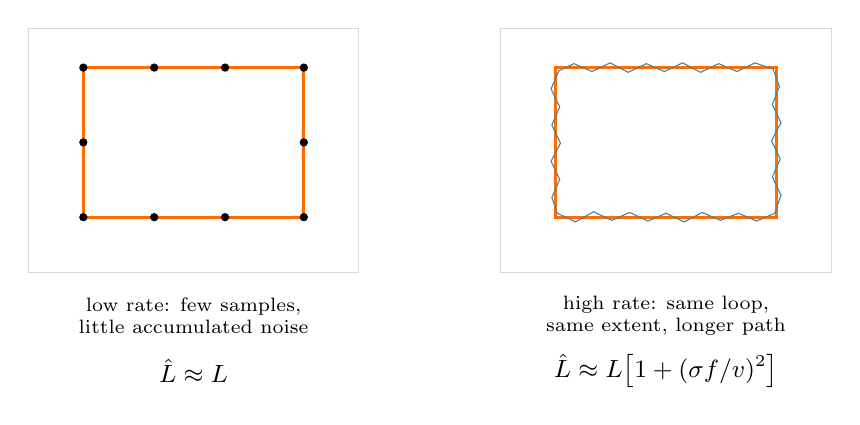
\begin{tikzpicture}[scale=1.0, every node/.style={font=\small}]
  \begin{scope}
    \draw[gray!30] (-0.2,-0.2) rectangle (4.0,2.9);
    \draw[orange!85!red, very thick] (0.5,0.5) -- (3.3,0.5) -- (3.3,2.4) -- (0.5,2.4) -- cycle;
    \foreach \p in {(0.5,0.5),(1.4,0.5),(2.3,0.5),(3.3,0.5),(3.3,1.45),(3.3,2.4),
                    (2.3,2.4),(1.4,2.4),(0.5,2.4),(0.5,1.45)}
      \fill[black] \p circle (1.5pt);
    \node[font=\scriptsize, align=center] at (1.9,-0.75)
      {low rate: few samples,\\little accumulated noise};
    \node at (1.9,-1.45) {$\hat L\approx L$};
  \end{scope}
  \begin{scope}[shift={(6.0,0)}]
    \draw[gray!30] (-0.2,-0.2) rectangle (4.0,2.9);
    \draw[orange!85!red, very thick] (0.5,0.5) -- (3.3,0.5) -- (3.3,2.4) -- (0.5,2.4) -- cycle;
    \draw[cyan!60!black, thin]
      (0.52,0.55) -- (0.75,0.44) -- (0.98,0.57) -- (1.21,0.46) -- (1.44,0.56)
      -- (1.67,0.45) -- (1.90,0.55) -- (2.13,0.44) -- (2.36,0.56) -- (2.59,0.46)
      -- (2.82,0.55) -- (3.05,0.45) -- (3.28,0.55) -- (3.36,0.78) -- (3.25,1.01)
      -- (3.35,1.24) -- (3.24,1.47) -- (3.36,1.70) -- (3.25,1.93) -- (3.34,2.16)
      -- (3.26,2.38) -- (3.03,2.46) -- (2.80,2.35) -- (2.57,2.45) -- (2.34,2.34)
      -- (2.11,2.46) -- (1.88,2.35) -- (1.65,2.45) -- (1.42,2.34) -- (1.19,2.46)
      -- (0.96,2.35) -- (0.73,2.45) -- (0.54,2.36) -- (0.44,2.13) -- (0.55,1.90)
      -- (0.45,1.67) -- (0.56,1.44) -- (0.44,1.21) -- (0.55,0.98) -- (0.45,0.75) -- cycle;
    \node[font=\scriptsize, align=center] at (1.9,-0.75)
      {high rate: same loop,\\same extent, longer path};
    \node at (1.9,-1.45) {$\hat L\approx L\bigl[1+(\sigma f/v)^{2}\bigr]$};
  \end{scope}
\end{tikzpicture}
\vspace{2mm}
\caption{Why cumulative path length must not be compared across sampling
rates. Both panels show the same physical loop with the same spatial extent;
the right-hand estimator merely samples it faster. Every additional sample
contributes its own noise excursion, so the measured path lengthens
quadratically in the sampling rate (Eq.~\ref{eq:pathinflation}) while the
extent is inflated only by the additive constant of
Eq.~\ref{eq:extentbias}. The two ratios quoted in
Fig.~\ref{fig:trajcomparison} differ for exactly this reason.}
\label{fig:pathinflation}
\end{figure}

The model is not decorative: it caught a real defect in the plotting script.
Path lengths were originally computed on the \emph{raw} traces, at their
native rates of $86$\,Hz (MINS) and $80$\,Hz (openVINS), and reported
$16.78$\,m for both, an apparently perfect agreement, printed as a title
above a panel whose two curves visibly separated. Recomputing on the common
$20$\,Hz base, the base the panel actually plots, gives $15.29$\,m and
$13.74$\,m. The raw agreement was a coincidence of two different noise
levels inflating two different true lengths onto the same number, and it had
been concealing a genuine $10\%$ discrepancy.

Eq.~\ref{eq:pathinflation} can be inverted to recover the per-sample noise
that produced the observed inflation, $\sigma=(v/f)\sqrt{\hat L/L-1}$, which
yields $0.43$\,mm per sample for MINS and $0.63$\,mm for openVINS. The
figure of $1.5\times$ more per-sample position noise on openVINS is
consistent with the qualitative behaviour recorded throughout this campaign,
and with the residual structure of panel~7, where the post-alignment error
is a pair of smooth $\pm0.5$\,m excursions rather than sample-to-sample
scatter: that is, a slowly varying disagreement in trajectory, sitting on
top of a much finer per-sample jitter.

\subsection{Ground-truth calibration: the first measurements on this
platform not made against another estimator}
\label{sec:july29calib}
Every quantitative statement in this chapter up to this point compares one
estimator against another. Section~\ref{sec:july29align} is explicit that
this cannot establish which of them is right. The July 29 session added the
missing ingredient: a tape measure and a protractor.

A calibration panel was added to the cockpit's Trajectory tab, backed by
\code{tools/calib\_terrain.py} for terminal use. The operator marks a start
pose, drives a known manoeuvre, marks the end pose, physically measures what
the robot actually did, and enters that measurement; the backend captures
what each of the four sources (wheel odometry, MINS, openVINS, and the
raw integrated gyroscope) believed had happened over exactly the same
interval, and reports the correction factor
\begin{equation}
g_{\text{source}}=\frac{\text{measured reality}}{\text{what the source believed}},
\label{eq:calibfactor}
\end{equation}
averaged over repeated passes with its standard deviation, since a single
pass conflates the systematic scale error being sought with the random
start-pose and slip errors of that particular run.

The rotational manoeuvre is the more valuable of the two, because it
measures a quantity that had never been observable on this platform. The
gyroscope obeys
\begin{equation}
\omega_{\text{meas}}=k\,\omega_{\text{true}}+b+\eta,
\label{eq:gyromodel}
\end{equation}
with scale error $k$, bias $b$ and noise $\eta$. The static
auto-calibration carried by \code{imu\_sanitizer.py} estimates $b$ from a
stationary robot, but at rest $\omega_{\text{true}}=0$, so Eq.~\ref{eq:gyromodel}
collapses to $\omega_{\text{meas}}=b+\eta$ and $k$ disappears from the
observation entirely. No amount of stationary data can determine it. This is
the limitation the sanitizer's own documentation had recorded as
outstanding. Integrating instead over a turn of known amplitude, with the
bias already removed,
\begin{equation}
\widehat{\Delta\theta}=\int_{0}^{T}\!\bigl(\omega_{\text{meas}}-b\bigr)\,dt
 = k\,\Delta\theta_{\text{true}},
\qquad\Longrightarrow\qquad
k=\frac{\widehat{\Delta\theta}}{\Delta\theta_{\text{true}}}=\frac{1}{g},
\label{eq:gyroscale}
\end{equation}
makes $k$ directly observable from a single turn against a protractor.

Measuring both directions separately is what turns the result into a
diagnosis rather than a number. Decomposing the two per-direction factors
into their symmetric and antisymmetric parts,
\begin{equation}
\bar g=\tfrac12\bigl(g_{\text{L}}+g_{\text{R}}\bigr),
\qquad
\delta=\tfrac12\bigl(g_{\text{L}}-g_{\text{R}}\bigr),
\label{eq:symantisym}
\end{equation}
a sensor scale error is necessarily sign-symmetric and appears wholly in
$\bar g$, whereas a mechanical defect (differential wheel slip, a
steering trim) reverses with the direction of travel and appears in
$\delta$. The two are therefore separable by measurement, and must be, since
correcting an antisymmetric fault with a symmetric gain would worsen one
direction while improving the other.

\begin{table}[htbp]
\centering
\caption{First ground-truth calibration pass, July 29. Factors are
$g=\text{reality}/\text{belief}$ as defined in Eq.~\ref{eq:calibfactor}; a
factor below unity means the source over-reports. The gyroscope's near-zero
antisymmetric component identifies a genuine scale error, while the wheel
odometry's is an order of magnitude larger and is mechanical in origin.
Single pass per direction: indicative, and superseded by the repeated
campaign recorded as item~36.}
\label{tab:calib29}
\begin{tabular}{lcccc}
\hline
Source & $g_{\text{left}}$ & $g_{\text{right}}$ & $\bar g$ (symmetric)
       & $\lvert\delta\rvert$ (antisym.) \\
\hline
Raw gyroscope   & $0.9344$ & $0.9313$ & $0.9329$ & $0.0016$ \\
MINS            & $0.9274$ & $0.9316$ & $0.9295$ & $0.0021$ \\
openVINS        & $0.9333$ & $0.9353$ & $0.9343$ & $0.0010$ \\
Wheel odometry  & $0.9325$ & $0.8920$ & $0.9123$ & $0.0203$ \\
\hline
\end{tabular}
\end{table}

Table~\ref{tab:calib29} reports the outcome. The gyroscope over-reports
rotation by $7.2\%$ ($k=1/\bar g=1.072$), and does so almost identically in
both directions: $\lvert\delta\rvert/\bar g=0.17\%$. By the argument above
this is a scale error, and a
\code{\textasciitilde gyro\_scale} parameter was added to the sanitizer to
carry the correction: defaulting to unity, that is, to no correction at
all, until a repeated campaign supersedes this single pass. Both inertial
estimators inherit the same $\sim7\%$, as they must, since both integrate
the same gyroscope. The wheel odometry is the outlier: its antisymmetric
component is more than ten times the gyroscope's, which is the signature of
the left-side drift already characterised in this campaign, and it is
precisely the fault that a global scale factor would entrench rather than
remove.

A methodological note belongs here, because it cost a full set of
measurements. The first calibration attempt entered the \emph{intended}
manoeuvre, ninety degrees, rather than the measured one. All four
sources agreed on $121.7^\circ$, and four independent sensors agreeing
against a single entered number is not a sensor fault. The robot had
overshot, and the exercise had measured how badly the platform tracks its
own command rather than how badly its sensors track reality. The two are
different quantities and only the second is a calibration. The interface was
revised accordingly: the worked example in the input placeholder was changed
from a round $90$ to a deliberately unround $87.5$, and a reminder that the
arrival instant is frozen, so the operator may take as long as the
measurement requires, is displayed alongside the field. A plausibility
guard now rejects any entry differing by more than a factor of five from the
median of what the sensors observed, on the reasoning that several
independent sensors do not err together by two orders of magnitude, so such
a disparity is a unit or typing error rather than a discovery.

\section{Field session, July 30: a thermal operating envelope, a native
absolute-error architecture, and the calibration blocker that gates both}
\label{sec:july30}

Two decisions shaped this session, and they pulled in opposite directions.
The first was to cancel the planned fan installation and deliberately accept
the thermal risk, in order to recover the colour stream that the beacon
detector needs at working distance. The second was to stop aligning
trajectories after the fact and instead measure error against a physical
anchor. The first decision produced a bounded, quantified failure; the second
produced an architecture that is complete but not yet validated, because a
calibration defect discovered the same evening invalidates every dimensional
quantity it would otherwise have produced. Both outcomes are reported here as
measured, including the one that contradicts the hypothesis under which the
session began.

\subsection{Thermal stress without active cooling: a characterised threshold
rather than a demonstration of resilience}
\label{sec:july30thermal}

The premise of the run was that the July 28 scheduling fix (\S\ref{sec:uartrtprio}), \code{SCHED\_FIFO} priority 25 on
\code{serial\_node}, together with the \code{LimitRTPRIO=50} drop-in on
\code{leo.service} without which the node refuses to start) had made the
serial link robust enough to survive thermal throttling. If true, active
cooling would be a comfort rather than a prerequisite, and the colour stream
could be restored immediately.

The first half of the run supported that premise. With \code{enable\_color}
restored and the Pi stabilised near $86\,^\circ$C, the instrumented vitals
held: the IMU delivered $82.8$\,Hz with $14$ gaps per $20$\,s, and wheel
odometry held $19.7$\,Hz, the same figure the scheduling fix had bought two
days earlier, now sustained under an additional camera load. On the evidence
available at that point, the fix was carrying the system through a thermal
regime that had previously destroyed it.

The second half refuted the generalisation. Later the same evening the entire
firmware chain fell silent, and the operator's report was that neither manual
nor autonomous driving responded. The measurements taken at that moment are
given in Table~\ref{tab:july30thermal}.

\begin{table}[htbp]
\centering
\small
\caption{Measured state at the two ends of the thermal envelope. The right
column is not a degradation of the left one: it is a different regime,
reached across roughly three degrees.}
\label{tab:july30thermal}
\begin{tabular}{@{}lcc@{}}
\toprule
Quantity & Hot run (stable) & Collapse \\
\midrule
Core temperature            & $\sim86\,^\circ$C & $89.1\,^\circ$C \\
\code{get\_throttled}       & \code{0xe0006}    & \code{0xe0006} \\
ARM clock                   & $600$\,MHz        & $600$\,MHz \\
Load average ($4$ cores)    & not measured & $8.85$ \\
\code{realsense2\_camera\_manager} & not measured & $185\,\%$ CPU \\
UART overruns (\code{oe})   & $137\,000$ (Jul 28) & $676\,751$ \\
\code{/firmware/wheel\_states} & $19.7$\,Hz & $0$\,Hz \\
\code{/imu/data\_raw}          & $82.8$\,Hz & $0$\,Hz \\
\code{/joint\_states}          & nominal    & $0$\,Hz \\
\code{serial\_node} state      & synchronised & \code{Lost sync}, $\sim15$\,s period \\
\bottomrule
\end{tabular}
\end{table}

\noindent\textbf{The causal chain, and why it presented as a control fault.}
The colour nodelet consumed $185\,\%$ of a four-core budget already carrying
two estimators' worth of publication traffic, driving the load average to
$8.85$, a factor $2.2$ oversubscription, while the clock remained pinned
at its $600$\,MHz throttle floor. Under that starvation the PL011 FIFO is not
serviced within the time a byte takes to arrive at $460\,800$\,baud, and the
overrun counter rose to $676\,751$, nearly five times the July 28 figure.
\code{rosserial} responds to a corrupted frame by renegotiating the topic
handshake, which under sustained overruns never completes before the next
corruption, producing the observed $15$-second \code{Lost sync} cycle. No
firmware topic survives that loop.

The diagnostic value of the symptom deserves emphasis, because it is
reusable. Manual and autonomous driving failed \emph{together}, and that
simultaneity is informative rather than alarming: the two modes share exactly
one component downstream of the finite-state machine, namely
\code{/serial\_node}, the sole subscriber of \code{/cmd\_vel}. A fault that
removes both at once therefore localises to the shared transport, and every
hypothesis concerning the mission logic, the web interface, or the command
bus can be discarded before it is tested. Confirmation was direct:
\code{rostopic info /cmd\_vel} showed the publisher and subscriber correctly
bound, while the backend's own health block independently reported
\code{odom: false}, \code{wheels: false} and \code{batt: false}. Commands were
leaving the backend and never reaching the CORE2.

\paragraph{A deadline model for the overrun, and why the failure has a
cliff.}
The overrun counter is not a vague indicator of stress. It counts a specific,
datable event: a byte arrived at the PL011 receiver while its receive FIFO was
already full, so the hardware discarded it. That makes the mechanism a
deadline problem, and it can be written down exactly.

The link runs at $B = 250\,000$ baud in 8N1 framing, so each byte occupies ten
bit periods and the inter-byte interval is
\begin{equation}
\tau_b \;=\; \frac{10}{B} \;=\; \frac{10}{250\,000} \;=\; 40\;\mu\text{s}.
\label{eq:bytetime}
\end{equation}
With a receive FIFO $N_f$ entries deep, the kernel must service the port
before $N_f$ further bytes accumulate, which gives the hard deadline
\begin{equation}
T_{\mathrm{dl}} \;=\; N_f\,\tau_b \;=\; 32 \times 40\;\mu\text{s}
              \;=\; 1.28\;\text{ms}.
\label{eq:fifodeadline}
\end{equation}
An overrun occurs if and only if the service latency $L$ exceeds
$T_{\mathrm{dl}}$. The exact FIFO depth matters less than it appears: halving
$N_f$ halves the deadline, and both values remain far below the scheduling
delays discussed next.

The latency decomposes into two terms with different causes:
\begin{equation}
L \;=\; \underbrace{L_{\mathrm{preempt}}}_{\text{when the task is chosen}}
   \;+\; \underbrace{\frac{f_{\max}}{f}\,C}_{\text{how long its work takes}},
\label{eq:latencysplit}
\end{equation}
where $C$ is the cost of the read path at full clock and $f_{\max}/f$ is the
frequency penalty. This split is the whole story of the July 28 fix and of its
July 30 limit. Promoting \code{serial\_node} to \code{SCHED\_FIFO} priority 25
attacks $L_{\mathrm{preempt}}$ alone: it removes the wait behind a run queue
that thermal throttling had made $8.85/4 = 2.21$ times oversubscribed.
It does nothing whatever to the second term, which throttling inflates by
\begin{equation}
\frac{f_{\max}}{f} \;=\; \frac{1500\;\text{MHz}}{600\;\text{MHz}} \;=\; 2.5 .
\label{eq:freqpenalty}
\end{equation}
The fix therefore buys margin only while $2.5\,C$ stays comfortably under
$1.28$\,ms, which is precisely the sense in which it holds at $86\,^\circ$C
and fails at $89\,^\circ$C.

\begin{figure}[htbp]
\centering
\begin{tikzpicture}[font=\small, >=Latex, scale=0.98]
  % --- arrivee des octets, cadencee par le CORE2 et non par le Pi ---
  \node[font=\scriptsize, anchor=east] at (-0.25,0) {bytes in};
  \foreach \x in {0,0.44,...,7.1} \draw[gray] (\x,-0.16) -- (\x,0.16);
  \draw[->] (0,0) -- (10.6,0) node[right, font=\scriptsize] {$t$};
  \draw[<->] (0,0.62) -- (0.44,0.62) node[midway, above, font=\scriptsize] {$\tau_b\!=\!40\,\mu$s};

  % --- echeance ---
  \draw[thick, densely dashed] (7.04,0.95) -- (7.04,-2.75);
  \node[anchor=south, font=\scriptsize, align=center] at (7.04,1.0)
       {$T_{\mathrm{dl}}\!=\!N_f\tau_b\!=\!1.28$\,ms\\(FIFO full)};

  % --- service, deux regimes ---
  \draw[very thick, accentblue] (0,-1.25) -- (4.6,-1.25);
  \fill[accentblue] (4.6,-1.25) circle (2.4pt);
  \node[accentblue, font=\scriptsize, anchor=west] at (7.35,-1.25)
       {$L<T_{\mathrm{dl}}$: port read, nothing lost};
  \node[font=\scriptsize, anchor=east] at (-0.25,-1.25) {$86\,^\circ$C};

  \draw[very thick, alertred] (0,-2.3) -- (7.04,-2.3);
  \draw[very thick, alertred, densely dotted] (7.04,-2.3) -- (9.1,-2.3);
  \node[alertred, font=\scriptsize, anchor=west] at (7.35,-2.62) {byte discarded};
  \node[font=\scriptsize, anchor=east] at (-0.25,-2.3) {$89\,^\circ$C};
  \draw[alertred, very thick] (6.86,-2.48) -- (7.22,-2.12);
  \draw[alertred, very thick] (6.86,-2.12) -- (7.22,-2.48);

  \node[font=\scriptsize, anchor=north west, align=left] at (0,-3.15)
      {Throttling does not slow the arrivals, which are clocked by the CORE2.
       It lengthens\\only the service bar, so the margin is consumed from one
       side alone.};
\end{tikzpicture}
\caption[UART deadline]{The overrun as a missed deadline. Bytes arrive every
$\tau_b = 40\,\mu$s; the FIFO grants $1.28$\,ms of slack. Thermal throttling
does not slow the arrivals, which are set by the CORE2's clock, it only
lengthens the service. The margin is therefore consumed from one side only.}
\label{fig:july30deadline}
\end{figure}

\paragraph{From a miss probability to a collapse.}
Treating successive deadlines as a Bernoulli sequence with miss probability
$p$, the measured rate after recovery fixes $p$ directly. Bytes arrive at
$B/10 = 25\,000$ per second, so fill events occur at
\begin{equation}
\nu \;=\; \frac{B}{10\,N_f} \;=\; \frac{25\,000}{32}
      \;=\; 781\;\text{s}^{-1},
\label{eq:fillrate}
\end{equation}
while the counter advanced by $553$ in $180$\,s, that is $3.07$\,s$^{-1}$.
Hence
\begin{equation}
p \;=\; \frac{3.07}{781} \;=\; 3.9\times10^{-3},
\label{eq:missprob}
\end{equation}
a miss on roughly one deadline in $260$. That figure is small, and on its own
it would suggest a system merely degraded rather than one that had stopped
entirely. The reconciliation is that \code{rosserial} does not tolerate
isolated losses gracefully: a corrupted frame forces a full topic
renegotiation, and the handshake itself must cross $M \approx 2\,000$ bytes
without a single overrun. Its success probability is therefore
\begin{equation}
P_{\mathrm{hs}}(p) \;=\; (1-p)^{M/N_f} \;=\; (1-p)^{62}.
\label{eq:handshake}
\end{equation}
At the measured $p = 3.9\times10^{-3}$ this gives $P_{\mathrm{hs}} = 0.78$:
the link recovers on the first or second attempt, which is exactly what the
targeted cycle achieved. Asking instead when recovery becomes improbable,
$P_{\mathrm{hs}} < 0.05$, gives
\begin{equation}
p^{\star} \;=\; 1 - 0.05^{1/62} \;=\; 4.7\times10^{-2},
\label{eq:pcrit}
\end{equation}
a factor of twelve above the measured value. This is the quantitative content
of the three-degree envelope. The system does not degrade smoothly into
uselessness; it crosses a threshold at which the recovery mechanism itself
stops working, and thereafter every renegotiation fails for the same reason
the previous one did. A twelvefold change in a latency margin is a small
thermal step, and it separates a rover that loses the occasional message from
one that answers no command at all.

\begin{figure}[htbp]
\centering
\begin{tikzpicture}[font=\small, >=Latex, xscale=1.0, yscale=1.0]
  \draw[->] (0,0) -- (9.6,0) node[below right, font=\scriptsize] {$p$ (miss probability)};
  \draw[->] (0,0) -- (0,4.3) node[left, font=\scriptsize] {$P_{\mathrm{hs}}$};
  \foreach \y/\l in {0/0, 2/0.5, 4/1.0} \draw (-0.08,\y) -- (0.08,\y) node[left=4pt, font=\scriptsize] {\l};
  \foreach \x/\l in {0/0, 3/0.02, 6/0.04, 9/0.06} \draw (\x,-0.08) -- (\x,0.08) node[below, font=\scriptsize] {\l};
  \draw[very thick, accentblue] plot[domain=0:9, samples=80]
       (\x, {4*pow(1-\x/150, 62)});
  \draw[dashed, gray] (0.585,0) -- (0.585,3.16) -- (0,3.16);
  \node[font=\scriptsize, anchor=west, accentblue] at (0.75,3.55)
       {measured: $p=3.9\times10^{-3}$, $P_{\mathrm{hs}}=0.79$};
  \draw[dashed, alertred] (7.05,0) -- (7.05,0.2);
  \node[font=\scriptsize, anchor=south west, alertred, align=left] at (5.4,0.45)
       {$p^{\star}=4.7\times10^{-2}$:\\recovery fails};
\end{tikzpicture}
\caption[Handshake cliff]{Equation~\ref{eq:handshake}: probability that a
\code{rosserial} topic renegotiation completes without an overrun. The
function is smooth, but the system's behaviour is not, because below the knee
a failed handshake is retried successfully within seconds, and above it every
retry fails. Twelve times the measured miss probability separates the two
regimes.}
\label{fig:july30cliff}
\end{figure}

\noindent\textbf{Recovery, and what it did not fix.} A targeted
\code{rosmon} cycle of \code{serial\_node} (not a stack restart, following
the July 22 lesson (\S\ref{sec:july22network}) that the surrounding
infrastructure is rarely the culprit) restored the chain to $17.1$\,Hz on
\code{wheel\_states}, $18.7$\,Hz on \code{wheel\_odom} and $79.3$\,Hz on the
IMU, with \code{SCHED\_FIFO} priority 25 correctly reapplied by the launch
wrapper. The recovery is nonetheless a reset, not a repair: three minutes
later, at $88.6\,^\circ$C and still throttled, the overrun counter had
advanced a further $553$ counts. The mechanism that produced the collapse was
running at undiminished rate.

\noindent\textbf{What this establishes, stated precisely.} It would be
convenient to record that the architecture proved resilient without active
cooling. The measurements do not support that claim, and a reader with access
to \code{serial\_node.log} would find the contradiction in one command. What
the session established is narrower and more useful: an \emph{operating
envelope}. The scheduling fix holds the serial link at $86\,^\circ$C under
full colour load, and does not hold it at $89\,^\circ$C. The usable margin is
therefore on the order of three degrees, with no headroom for ambient
variation, and sustained operation above roughly $88\,^\circ$C requires manual
intervention at intervals of tens of minutes. A threshold measured on both
sides is a stronger result than an absence of failure asserted from a single
favourable sample, but it is a result that mandates the fan, rather than
retiring it.

\noindent\textbf{A correction to an earlier measurement.} Appendix
\S\ref{ap:repro-thermal} records that disabling the colour stream produced
zero thermal improvement, and concluded from this that the software levers
were exhausted. That observation was real but its interpretation was wrong:
colour had been disabled at driver level, so the stream being switched off
was already absent and the measurement compared a configuration with itself.
The $185\,\%$ CPU figure recorded above is the first direct measurement of
what the colour nodelet actually costs, and it is the dominant term in the
thermal budget. The lever exists; the July 30 decision was to spend it
deliberately, which is a different matter from its not existing.

\subsection{From a posteriori alignment to a native absolute error: the
beacon-anchored TF bridge}
\label{sec:july30bridge}

Every error figure in this campaign so far has been a residual after
alignment. Both estimates and reference are expressed in frames whose
relative pose is unknown, so the two point sets are registered (rigidly by
Kabsch, or with a scale degree of freedom by Umeyama) and the residual of
that registration is reported. \S\ref{sec:july29align} derived the exact
price of the scale freedom,
\begin{equation}
\varepsilon^{2}_{\mathrm{rig}} - \varepsilon^{2}_{\mathrm{sim}}
  = \sigma_{p}^{2}\,(s^{\star}-1)^{2},
\label{eq:july30scaleprice}
\end{equation}
which makes explicit that a similarity fit absorbs a systematic scale error
into a free parameter and reports what remains. The rigid fit removes one
degree of freedom but still absorbs an arbitrary rotation and translation.
In both cases the quantity reported is a residual \emph{after} the estimator
has been given the benefit of an optimal transform it never had access to
during the run. That is a legitimate measure of shape agreement, and it is
not an absolute error.

\paragraph{What alignment removes, written as a projection.}
The objection can be made precise, and once it is, the size of the effect
follows without any experiment. Let $\{\hat{\mathbf{p}}_k\}_{k=1}^{N}$ be the
estimated positions, $\{\mathbf{p}_k\}$ the reference, and
$\mathbf{e}_k = \hat{\mathbf{p}}_k - \mathbf{p}_k$ the error we should like to
report. Stack them into $\mathbf{e} \in \mathbb{R}^{3N}$.

Alignment does not report $\lVert\mathbf{e}\rVert$. It reports what survives
an optimisation over the transform group. Writing the fitted rotation near
identity as $R \approx I + [\delta\boldsymbol{\omega}]_\times$, the
translation as $\delta\mathbf{t}$ and the similarity scale as
$s = 1 + \delta s$, the post-alignment residual at index $k$ is
\begin{equation}
\mathbf{r}_k \;=\; \mathbf{e}_k
  \;-\;\bigl(\delta\mathbf{t}
  \;+\;\delta\boldsymbol{\omega}\times\mathbf{p}_k
  \;+\;\delta s\,\mathbf{p}_k\bigr) \;+\; O(\lVert\delta\rVert^{2}).
\label{eq:gaugeresidual}
\end{equation}
The bracketed term ranges over a linear subspace of $\mathbb{R}^{3N}$, spanned
by seven vectors evaluated along the trajectory:
\begin{equation}
\mathcal{G} \;=\; \operatorname{span}\Bigl\{
  \underbrace{(\mathbf{\hat e}_i)_k}_{\text{3 translations}},\;
  \underbrace{(\mathbf{\hat e}_i\times\mathbf{p}_k)_k}_{\text{3 rotations}},\;
  \underbrace{(\mathbf{p}_k)_k}_{\text{1 scale}}
  \Bigr\},\qquad i=1,2,3 .
\label{eq:gaugespace}
\end{equation}
Least squares over these parameters is exactly orthogonal projection onto the
complement, so what the campaign has been reporting is
\begin{equation}
\varepsilon^{2}_{\mathrm{sim}}
  = \tfrac{1}{N}\bigl\lVert P_{\mathcal{G}^{\perp}}\,\mathbf{e}\bigr\rVert^{2},
\qquad
\varepsilon^{2}_{\mathrm{rig}}
  = \tfrac{1}{N}\bigl\lVert P_{\mathcal{G}_{6}^{\perp}}\,\mathbf{e}\bigr\rVert^{2},
\label{eq:projected}
\end{equation}
with $\mathcal{G}_6 \subset \mathcal{G}$ the rigid subspace obtained by
dropping the scale generator. Equation~\ref{eq:july30scaleprice} is the
Pythagorean difference between these two projections, which is why it is an
identity rather than an empirical finding.

\paragraph{Why this is not a small correction.}
Since projection can only shorten a vector,
\begin{equation}
\varepsilon^{2}_{\mathrm{sim}} \;\le\;
\varepsilon^{2}_{\mathrm{rig}} \;\le\;
\varepsilon^{2}_{\mathrm{abs}} \;=\; \tfrac{1}{N}\lVert\mathbf{e}\rVert^{2},
\label{eq:lowerbound}
\end{equation}
so \emph{every} error figure reported in this campaign to date is a lower
bound on the true error, never an overestimate. The gap is
$\lVert P_{\mathcal{G}}\mathbf{e}\rVert^{2}/N$, and its size depends on how
much of the error happens to lie in $\mathcal{G}$.

That is where the argument bites. The dominant failure modes of a
visual-inertial estimator are a slowly accumulating heading error and a slowly
drifting metric scale. Their error signatures are
$\delta\boldsymbol{\omega}\times\mathbf{p}_k$ and $\delta s\,\mathbf{p}_k$,
which are not merely close to $\mathcal{G}$: by
Eq.~\ref{eq:gaugespace} they are basis vectors \emph{of} $\mathcal{G}$. An
alignment-based metric is therefore blind, by construction, to precisely the
quantities the comparison exists to measure. A perfectly shaped trajectory
rotated by ten degrees and stretched by five percent scores a residual of
zero.

\begin{figure}[htbp]
\centering
\begin{tikzpicture}[font=\small, >=Latex, scale=1.05]
  \fill[accentblue!8] (-0.3,-0.3) -- (6.2,-0.3) -- (7.0,1.1) -- (0.5,1.1) -- cycle;
  \node[accentblue, font=\scriptsize, anchor=west] at (4.1,0.35)
       {$\mathcal{G}$: rotation, translation, scale};
  \draw[->, very thick] (1.2,0.15) -- (3.6,3.3) node[midway, left=3pt] {$\mathbf{e}$};
  \draw[->, very thick, alertred] (1.2,0.15) -- (3.6,0.15)
        node[midway, below=2pt, font=\scriptsize, alertred] {$P_{\mathcal{G}}\mathbf{e}$ absorbed};
  \draw[->, very thick, accentblue] (3.6,0.15) -- (3.6,3.3)
        node[midway, right=3pt, font=\scriptsize, accentblue]
        {$P_{\mathcal{G}^{\perp}}\mathbf{e}$ reported};
  \draw (3.35,0.15) rectangle (3.6,0.4);
  \node[font=\scriptsize, align=left, anchor=north west] at (-0.3,-0.6)
      {A yaw drift or a scale drift lies \emph{inside} $\mathcal{G}$,\\
       so alignment reports zero for it. The bridge measures
       $\lVert\mathbf{e}\rVert$ itself.};
\end{tikzpicture}
\caption[Gauge subspace]{Alignment reports only the component of the error
orthogonal to the transform group. The absorbed component is not noise: it
carries the heading and scale drift that a visual-inertial comparison is
meant to expose.}
\label{fig:july30gauge}
\end{figure}

\paragraph{The bridge removes the projection rather than shrinking it.}
Anchoring does not estimate a better transform, it removes the freedom to
estimate one at all. The static \code{beacon\_link} $\to$ \code{odom}
transform $T_{bo}$ is captured once, physically, before the run and held
constant, so the reported quantity is
\begin{equation}
\varepsilon^{2}_{\mathrm{abs}}
  \;=\;\frac{1}{N}\sum_{k=1}^{N}
  \bigl\lVert\, T_{bo}\,\hat{\mathbf{p}}_k - \mathbf{q}_k \,\bigr\rVert^{2},
\qquad \dim\mathcal{G} = 0,
\label{eq:absoluteerror}
\end{equation}
where $\mathbf{q}_k$ is the optically observed robot position in the beacon
frame. No parameter is fitted at measurement time, the inequality chain of
Eq.~\ref{eq:lowerbound} collapses to an equality at its right-hand end, and
the heading and scale drift that $\mathcal{G}$ was hiding become observable.

The alternative implemented on July 30 is to give the system a physical
anchor and measure against it directly.
\code{catkin\_ws/src/leo\_navigation/scripts/carolus\_tf\_bridge.py} publishes
the transform \code{camera\_frame} $\to$ \code{carolus\_raw} from the live
optical detection, together with a static \code{beacon\_link} $\to$
\code{odom} transform captured once, at anchoring time, and thereafter held
fixed. From these it derives two topics, \code{/odom\_in\_beacon} and
\code{/carolus\_in\_beacon}. Both carry the \emph{robot's} pose expressed in
the beacon frame, reached by two independent paths: the first through the
odometric and estimator chain, the second through the optical detection of a
fixed object. Their instantaneous difference is an absolute error, containing
no fitted transform, no scale parameter and no free variables: the
alignment is performed once, physically, by the act of anchoring, rather than
numerically and repeatedly by an optimiser with the answer in hand.

\noindent\textbf{A constraint the implementation had to respect.} A frame in
a \code{tf2} tree has exactly one parent. It is tempting to have the bridge
publish the full body chain in the beacon frame, and an early revision did
precisely that; the result was a second parent for \code{base\_link} and a
tree that \code{tf2} resolves nondeterministically, announced only by
intermittent \code{TF\_OLD\_DATA} warnings. The bridge therefore publishes
\emph{only} the camera-to-beacon observation and the static anchor, and
exposes the body chain behind a \code{\textasciitilde publish\_body\_chain}
parameter that defaults to false and emits a \code{logerr} when enabled. The
same constraint drove the linearisation of the main tree to a strict
\code{odom} $\to$ \code{base\_footprint} $\to$ \code{base\_link} chain
(\S\ref{ap:trap-tf}).

\noindent\textbf{Status, stated without inflation.} The bridge is written,
executable, and deliberately absent from every launch file, so that it is
started explicitly by an operator who intends to use it and cannot silently
perturb an unrelated run. It has been executed and observed to publish. It
has \emph{not} been validated against recorded data: no run to date has
recorded \code{/odom\_in\_beacon} or \code{/carolus\_in\_beacon}, and the
trajectory bags available at the time of writing contain only
\code{/mins/imu/odom}, \code{/ov\_msckf/odomimu}, \code{/robot\_pose\_fused}
and \code{/firmware/wheel\_odom}. No absolute-error figure is therefore
reported in this document, and the architecture above should be read as a
method awaiting its first measurement rather than as a result.

\subsection{The calibration defect that gates the measurement}
\label{sec:july30intrinsics}

The reason that first measurement was not simply taken is a defect found
while verifying the detector's outputs. The intrinsic parameters used by
\code{carolus\_astrobee\_rex}, read live from the parameter server, do not
correspond to the stream it is consuming.

\begin{table}[htbp]
\centering
\small
\caption{Detector intrinsics against the intrinsics of the stream actually
published. The two describe different optical configurations.}
\label{tab:july30intrinsics}
\begin{tabular}{@{}lcc@{}}
\toprule
Parameter & \code{carolus\_astrobee\_rex} & \code{/camera/color/camera\_info} \\
\midrule
Stream size & (calibrated at $1280\times720$) & $640\times480$ \\
$f_x$ & $644.12$ & $380.35$ \\
$f_y$ & $645.29$ & $379.36$ \\
$c_x$ & $\mathbf{643.47}$ & $320.40$ \\
$c_y$ & $372.52$ & $243.72$ \\
\bottomrule
\end{tabular}
\end{table}

\noindent The decisive entry is $c_x = 643.47$ on an image $640$ pixels wide.
The principal point lies outside the image altogether, which is not a
tolerance question but a categorical inconsistency: the calibration was
performed at $1280\times720$, where the D455 colour sensor delivers its full
$90^\circ$ horizontal field, and is being applied to a $640\times480$ stream
which the driver crops to roughly $80^\circ$. The two are not related by a
scale factor, so no rescaling of the stored parameters can repair them.

The consequence is quantifiable without any experiment. A beacon imaged at
the true optical centre, pixel $(320, 240)$, is interpreted by the detector
as lying at
\begin{equation}
\alpha = \arctan\!\left(\frac{320 - 643.47}{644.12}\right) = -26.7^\circ,
\qquad
\beta  = \arctan\!\left(\frac{240 - 372.52}{645.29}\right) = -11.6^\circ,
\label{eq:july30bearingerror}
\end{equation}
in azimuth and elevation respectively. A target dead ahead is reported
nearly $27^\circ$ off-axis. Every range and bearing derived from this
projection, and therefore every position the bridge would express in the
beacon frame, is invalid as a metric quantity. The six-degree-of-freedom
readings observed on the cockpit during this session (of order
$1.2$\,m in $x$ and $-0.55$\,m in $y$) are consistent, self-coherent and
metrically meaningless.

\paragraph{Propagating the defect through the pinhole model.}
Equation~\ref{eq:july30bearingerror} gives the bearing error at one pixel. The
full consequence is better seen by propagating the wrong parameters through
the projection itself. The pinhole model maps a point
$(X,Y,Z)$ in the camera frame to
\begin{equation}
u = f_x\frac{X}{Z} + c_x, \qquad v = f_y\frac{Y}{Z} + c_y,
\label{eq:pinhole}
\end{equation}
and the detector inverts it. Two quantities matter downstream: how far the
beacon is, and where it is laterally.

\smallskip\noindent\textit{Range.} For a beacon of known physical extent $L$
subtending $w$ pixels, similar triangles give $Z = f_x L / w$. The estimated
range therefore scales linearly with the assumed focal length, and the error
is a pure multiplicative bias independent of distance, orientation and pixel
position:
\begin{equation}
\frac{\hat Z}{Z} \;=\; \frac{f'_x}{f_x} \;=\; \frac{644.12}{380.35}
  \;=\; 1.693 .
\label{eq:rangebias}
\end{equation}
Every range this detector reports is inflated by $69.3\,\%$. A beacon at one
metre is reported at $1.69$\,m, and no averaging, filtering or repetition
reduces the error, because it is not noise.

\smallskip\noindent\textit{Lateral position.} Combining
Eq.~\ref{eq:pinhole} with $Z = f_x L/w$ gives
\begin{equation}
X \;=\; \frac{(u - c_x)\,Z}{f_x} \;=\; \frac{(u-c_x)\,L}{w},
\label{eq:lateral}
\end{equation}
in which the focal length has cancelled. The lateral estimate is governed
\emph{entirely} by the principal point, and the induced offset
\begin{equation}
\Delta X \;=\; \frac{(c_x - c'_x)\,L}{w}
      \;=\; -\,\frac{323.07\,L}{w}
\label{eq:lateralbias}
\end{equation}
is a constant translation of the whole scene, identical for every beacon
position in the image. This is the most treacherous property of the defect:
a rigid lateral offset produces a beacon track that is smooth, repeatable and
internally consistent, and therefore looks exactly like good data. For an
object of extent $L$ subtending $w = 40$ pixels, a plausible working figure at
this range, Eq.~\ref{eq:lateralbias} predicts an offset of $8.08\,L$ metres,
which for a beacon $0.15$\,m across is $1.21$\,m. The cockpit reading observed
during this session was $x = 1.18$\,m. The agreement should not be read as a
confirmed diagnosis, since $L$ and $w$ were not measured at the instant of the
reading, but it does establish that the observed value is of the same order as
the artefact and cannot be separated from it.

\begin{figure}[htbp]
\centering
\begin{tikzpicture}[font=\small, >=Latex, scale=0.95]
  \draw[very thick] (0,-1.6) -- (0,1.6);
  \node[anchor=south, font=\scriptsize] at (0,1.65) {sensor, $640$ px wide};
  \foreach \y/\l in {1.5/0, 0/320, -1.5/639}
     \draw (-0.12,\y) -- (0.12,\y) node[left=3pt, font=\scriptsize] {\l};
  \fill[accentblue] (0,0) circle (2.2pt);
  \node[accentblue, font=\scriptsize, anchor=east] at (-0.75,0.32) {$c_x = 320.4$};
  \fill[alertred] (0,-3.05) circle (2.2pt);
  \node[alertred, font=\scriptsize, anchor=east] at (-0.75,-3.05)
       {$c'_x = 643.5$, off the sensor};
  \draw[dotted, alertred, thick] (0,-1.6) -- (0,-3.2);
  \coordinate (P) at (7.4,0);
  \draw[accentblue, thick] (0,1.5) -- (P) -- (0,-1.5);
  \node[accentblue, font=\scriptsize] at (4.5,1.15) {true cone, $80^\circ$};
  \draw[alertred, thick, dashed] (0,1.5) -- (7.4,-3.05) -- (0,-1.5);
  \node[alertred, font=\scriptsize, anchor=west] at (4.3,-2.35)
       {assumed cone, $90^\circ$, axis displaced};
  \draw[->, thick] (0,0) -- (7.9,0) node[right, font=\scriptsize] {optical axis};
  \draw[<->, gray] (7.4,0) -- (7.4,-3.05)
       node[midway, right=2pt, font=\scriptsize, gray] {$\Delta$ bearing $=26.7^\circ$};
\end{tikzpicture}
\caption[Intrinsics mismatch]{The stored calibration describes a different
camera from the one publishing frames. Its principal point falls below the
sensor's lower edge, so the assumed optical axis leaves the field of view
entirely and a target on the true axis is reported $26.7^\circ$ off it. The
two cones also differ in aperture, which is why no rescaling of the stored
parameters can reconcile them.}
\label{fig:july30cones}
\end{figure}

\noindent Because the range bias of Eq.~\ref{eq:rangebias} is multiplicative
and the lateral bias of Eq.~\ref{eq:lateralbias} is additive, their combined
effect on a beacon-frame trajectory is a similarity transform: a scaling by
$1.693$ composed with a fixed translation. That is a member of the very group
$\mathcal{G}$ of Eq.~\ref{eq:gaugespace}. The irony is exact and worth
stating plainly. The bridge exists to escape the gauge freedom that alignment
hides errors in, and the uncalibrated camera injects an error lying squarely
inside that same subspace. Until the intrinsics are corrected, an
alignment-based comparison would silently absorb the defect while the absolute
measurement would report it in full, so the two methods cannot even be
cross-checked against one another.

This is why \S\ref{sec:july30bridge} reports no error figure. The
architecture is sound and the anchor is physical, but the sensor model
feeding it is wrong by a margin that dwarfs the quantity being measured.
Re-calibrating the colour camera at its operating resolution is consequently
the single blocking prerequisite for the entire absolute-error programme, and
is recorded as such in Table~\ref{tab:openitems} and in
\S\ref{ap:next-intrinsics}.

\section{Field session, August 5: a rewritten guard, a diagnosed tilt, and
the first rectangle closed}
\label{sec:aug05}

This session executed the rectangle protocol requested directly by the
supervisor: a physical rectangle, taped and tape-measured at
$6.405\,\text{m}\times3.455\,\text{m}$, driven once trusting MINS and once
trusting openVINS, each compared against the tape measurement rather than
against each other (\S\ref{ap:repro-mins-guide}--\S\ref{ap:repro-rect-compare}
give the operator-facing procedure; what follows is the reasoning and the
mathematics behind what that procedure actually measured). Three findings
came out of it, in the order they were forced by the data rather than the
order that would read best: a load-bearing bug in the pose-fusion guard, found
and fixed only because the rectangle test happened to drive through it; a
tilt in the IMU mount that a decade of prior sessions never had reason to
isolate; and, finally, the rectangle itself, closed cleanly by MINS and not
at all by openVINS, for reasons the first two findings and the platform's
thermal envelope (\S\ref{ap:repro-hitrun}) explain jointly.

\subsection{The pose-fusion guard: a false floor, then a true one}
\label{sec:aug05guard}
\code{pose\_selector.py}'s plausibility guard has existed since 2026-07-13 for
a specific, narrow reason: during a camera dropout an estimator coasts on
inertial propagation alone, and a doubly-integrated accelerometer bias can
move the served pose by metres per second on a rover that tops out near
$0.4$\,m/s. The guard compares each incoming pose against the last
\emph{accepted} one and freezes the served output the instant the implied
speed exceeds a threshold,
\begin{equation}
v_k \;=\; \frac{\lVert \mathbf{p}_k - \mathbf{p}_{\text{ref}}\rVert}{t_k - t_{\text{ref}}},
\qquad
v_k > v_{\max}=1.5\ \text{m/s} \;\Rightarrow\; \text{reject},
\label{eq:guardspeed}
\end{equation}
re-anchoring the correction transform once the source is calm again so the
served frame stays continuous through the excursion. It had never been
exercised by a full driven loop before this session, only by the camera-loss
transients it was built for.

\paragraph{Symptom.} Driving the rectangle with openVINS as the served
source, the cockpit's trajectory display froze the instant the rover moved,
recovered while stationary, and froze again on the next turn.
\code{/robot\_pose\_fused} dropped to $\sim\!2$\,Hz with the trail buffer
stuck at a handful of points, and the guard's own log was saturated:
\begin{center}\ttfamily\footnotesize
[pose\_selector] pose VINS invraisemblable (17.3 m/s) --- pose servie GELEE\\{}
[pose\_selector] source VINS calmee apres 0.0 s d'excursion --- re-ancree
\end{center}
alternating several times per second. Nothing here is exotic: it is
Eq.~\ref{eq:guardspeed} doing exactly what it was written to do, on a
$17.3\,\text{m/s}$ reading impossible for this platform. What was wrong was
the diagnosis that followed, not the guard.

\paragraph{A hypothesis that measurement refused.} The first candidate
explanation was the floor on the denominator of Eq.~\ref{eq:guardspeed},
$\Delta t = \max(10^{-3}\,\text{s},\, t_k - t_{\text{ref}})$: at $90$\,Hz the
true sample interval is close to $11$\,ms, so if two timestamps ever landed
within the $1$\,ms floor, an entirely ordinary few-centimetre step would read
as tens of metres per second. Five hundred and ninety-two consecutive
openVINS messages, captured with the rover stationary, refuted it directly:
median $\Delta t = 11.00$\,ms, minimum $9.00$\,ms, zero samples under
$4$\,ms, worst speed implied at the $1$\,ms floor only $0.3$\,m/s. The
hypothesis is recorded here specifically because it did not survive contact
with data --- the discipline this report tries to hold throughout
(\S\ref{sec:tuning}) is to say so plainly rather than let a plausible guess
stand in for a measured cause.

\paragraph{The real mechanism, found by capturing the rover in motion.}
Sampling $2020$ consecutive openVINS messages while the rectangle was
actually being driven told a different story: timing stayed clean (median
$\Delta t=11.0$\,ms, minimum $9.0$\,ms, matching the static capture), but
$8.3\,\%$ of consecutive-sample speeds computed by Eq.~\ref{eq:guardspeed}
exceeded $v_{\max}$, the single worst case a $4.23$\,cm step inside a
$9$\,ms interval --- $4.7$\,m/s by the formula, and a real, correctly-timed
measurement. An MSCKF applies its visual-update corrections
\emph{discretely}, at each new keyframe; a few centimetres of legitimate
correction landing inside one $9$\,ms sample interval is the filter working
as designed, not the rover teleporting. Eq.~\ref{eq:guardspeed}, evaluated
between consecutive samples, cannot tell that step apart from the runaway it
exists to catch: both are large numerators over a small, fixed denominator.

\paragraph{Two independent defects, two independent fixes.} Diagnosing the
mechanism separated what had looked like one bug into two, addressed in two
commits.

\emph{Latch tolerance.} A single rejected sample latched the frozen state
immediately, and the frozen branch published nothing at all --- a bare
\code{return} --- so every consumer of \code{/robot\_pose\_fused} (the
cockpit display, the rosbag recorder, any rate-based health check) lost its
input the instant the guard fired, which is the entire visible symptom above.
Both are now additive changes only, applied without weakening
Eq.~\ref{eq:guardspeed}'s acceptance rule: a sample over threshold is still
never written into the trace, the correction transform, or the reference
pose, so no rejected sample can ever reach the trajectory or a downstream
consumer as if it were accepted. What changes is what happens to a rejection.
\begin{center}
\begin{tikzpicture}[font=\scriptsize, node distance=11mm and 18mm,
  st/.style={draw, rounded corners=3pt, minimum width=24mm, minimum height=8mm, fill=black!3, align=center},
  arr/.style={-{Stealth[length=2mm]}}]
\node[st, fill=accentblue!8, draw=accentblue] (sane) {SANE\\served fresh};
\node[st, right=of sane] (reject) {sample over $v_{\max}$};
\node[st, below=of reject, fill=alertred!10, draw=alertred] (insane) {INSANE\\held pose served,\\cov.\ $=10^6$};
\draw[arr] (sane.east) -- (reject.west);
\draw[arr] (reject) -- node[right]{3 consecutive} (insane);
\draw[arr] (reject.north) to[out=90,in=90] node[above]{$<3$: discard sample, stay SANE} (sane.north);
\draw[arr] (insane) to[out=180,in=270] node[left, align=right]{next sane sample:\\re-anchor} (sane.south);
\end{tikzpicture}
\end{center}
An isolated spike --- one to two consecutive rejections, the discrete-update
case above --- no longer latches anything: the sample is discarded and the
next one is judged on its own merits. Only a \emph{sustained} run of
\code{spike\_tolerance}$=3$ consecutive rejections ($\approx 33$\,ms at
$90$\,Hz) declares the source insane, at which point the last known-good pose
is republished with its diagonal covariance forced to $10^6$ --- not a
fabricated position, the last real measurement every consumer already held by
default, now still arriving so a rate check can tell ``source frozen, topic
alive'' apart from ``node dead, topic silent''. Replayed against the driving
capture as a pure decision-table exercise (Table~\ref{tab:guardreplay}):
normal traffic keeps every sample flowing, an isolated spike no longer trips
the latch, and a sustained run still does.

\begin{table}[htbp]
\centering\small
\begin{tabular}{lccc}
\toprule
Scenario & Fresh & Held & Latched? \\
\midrule
Normal drive (20 samples)          & 20 & 0  & no \\
Isolated spike (1 of 20)           & 19 & 1  & \textbf{no} (was: yes) \\
Sustained divergence (10 of 20)    & 10 & 10 & yes (unchanged) \\
\bottomrule
\end{tabular}
\caption{Guard state-machine replay, latch-tolerance fix only. The isolated
case is the one that changed: it neither latches nor is silently invented ---
the sample is discarded, the topic keeps publishing.}
\label{tab:guardreplay}
\end{table}

\emph{The metric itself.} The latch fix alone still evaluates
Eq.~\ref{eq:guardspeed} between \emph{consecutive} samples, so the same
$4.23$\,cm/$9$\,ms correction still individually fails the test every time it
occurs; it simply no longer freezes the topic. The deeper fix replaces the
denominator's reference point: instead of the immediately preceding sample,
compare against the oldest still-accepted pose inside a sliding window of
duration $T=0.1$\,s,
\begin{equation}
v_k \;=\; \frac{\lVert \mathbf{p}_k - \mathbf{p}_{k-w}\rVert}{t_k - t_{k-w}},
\qquad
t_k - t_{k-w} \;\le\; T ,
\label{eq:guardwindow}
\end{equation}
falling back to the immediate predecessor while less than $T$ of history
exists (start-up, and immediately after a re-anchor, where the window is
deliberately cleared: the frame just changed, so old entries are not
comparable to the new one). The same displacement read against a longer
baseline reads a smaller speed for exactly the same physical event, because a
discrete correction of fixed size $\delta$ contributes $\delta/T$ once $T$
exceeds the interval it occurred in, while a \emph{sustained} runaway of
speed $v$ still covers $vT$ within the same window --- the window shrinks the
correction's apparent speed roughly in proportion to $T$, but leaves a true
runaway's apparent speed unchanged. The $4.23$\,cm case: $4.7$\,m/s at
$T=11$\,ms, $0.42$\,m/s at $T=100$\,ms, comfortably under $v_{\max}$.

Replayed on synthetic traffic built to match the measured statistics ($0.3$\,m/s
mean drift plus $2$--$4$\,cm discrete corrections at the observed rate,
$900$ samples at $90$\,Hz) and separately on a sustained $6$\,m/s runaway,
Table~\ref{tab:guardwindow} is the result: false rejections disappear, true
divergence detection is unchanged.

\begin{table}[htbp]
\centering\small
\begin{tabular}{lcc}
\toprule
Baseline $T$ & False rejects (normal traffic, /900) & Detected (6\,m/s runaway, /200) \\
\midrule
$11$\,ms (consecutive-sample) & $46$ ($5.1\,\%$) & $199$ \\
$100$\,ms (Eq.~\ref{eq:guardwindow}) & $\mathbf{0}$ & $199$ \\
\bottomrule
\end{tabular}
\caption{The baseline-window fix (Eq.~\ref{eq:guardwindow}), verified by
replay before deployment. A sustained runaway is caught identically at both
baselines because it accumulates displacement proportionally to $T$, unlike
a discrete correction of fixed size.}
\label{tab:guardwindow}
\end{table}

Deployed and re-measured live: \code{/robot\_pose\_fused} publishing at
$76$--$83$\,Hz through driven turns that previously froze it within the first
second.

\subsection{An uncommanded IMU tilt}
\label{sec:aug05tilt}
With the rover confirmed stationary --- wheel velocities
$[0,0,0,0]$, zero \code{/cmd\_vel} on every axis --- \code{/mins/imu/odom}
still drifted $0.75$\,m in $15$\,s ($50$\,mm/s) and \code{/ov\_msckf/odomimu}
$11.4$\,m in the same window ($765$\,mm/s), both far outside protocol
T1.1's $1$\,mm/s pass criterion (\S\ref{ap:repro-t11}). The gyroscope was
clean at rest ($0.0002$\,rad/s about every axis), so the search moved to the
accelerometer.

\paragraph{Magnitude checks out; direction does not.} Thirteen samples of
\code{/imu/data\_clean}, stationary, gave
$\bar{\mathbf{a}} = (1.1356,\ 0.6689,\ 9.6810)$\,m/s$^2$
($\sigma = 0.015, 0.014, 0.019$). Its norm,
\begin{equation}
\lVert\bar{\mathbf{a}}\rVert = \sqrt{1.1356^2+0.6689^2+9.6810^2}
 = 9.7703\ \text{m/s}^2,
\label{eq:accnorm}
\end{equation}
sits $0.0197$\,m/s$^2$ ($0.2\,\%$) below Melbourne FL local gravity
($9.790$\,m/s$^2$, used throughout this report). That confirms
\code{accel\_scale}$=1.1186$ (\S\ref{ap:repro-ourcode}) is doing its job: the
much larger, already-documented magnitude defect it corrects for
($8.7525$\,m/s$^2$ raw, $-10.6\,\%$) is not what is happening here. This is a
second, independent finding: the sensor reports the right \emph{amount} of
specific force, from the wrong \emph{direction}.

\paragraph{Decomposing the direction.} A stationary IMU measures $-\mathbf{g}$
expressed in its own frame; with the yaw component unobservable from a single
static reading, the roll and pitch it implies follow the standard
aerospace decomposition,
\begin{equation}
\text{roll} = \operatorname{atan2}(a_y,\,a_z), \qquad
\text{pitch} = \operatorname{atan2}\!\bigl(-a_x,\ \sqrt{a_y^2+a_z^2}\bigr),
\label{eq:rollpitch}
\end{equation}
in the REP-103 body convention ($x$ forward, $y$ left, $z$ up). Substituting
$\bar{\mathbf{a}}$:
\begin{equation}
\text{roll} = \operatorname{atan2}(0.6689,\,9.6810) = +3.95^\circ, \qquad
\text{pitch} = \operatorname{atan2}(-1.1356,\,9.7048) = -6.67^\circ .
\label{eq:rollpitchval}
\end{equation}
\begin{center}
\begin{tikzpicture}[font=\scriptsize, scale=1.0]
  % Angle drawn at 25 deg, not the measured 6.67 deg: at true scale the two
  % vectors overlap and the figure is illegible. Exaggeration is stated
  % explicitly, in the figure and in the caption, alongside the real value.
  \draw[->, thick] (0,0) -- (0,2.6) node[above right=1pt]{$z_{\text{body}}$};
  \draw[->, thick] (0,0) -- (2.4,0) node[right]{$x_{\text{body}}$};
  \draw[->, thick, dashed, alertred] (0,0) -- (0,2.3)
    node[above left=1pt]{$-\mathbf g$, if level};
  \draw[->, very thick, accentblue] (0,0) -- ({2.3*sin(25)},{2.3*cos(25)})
    node[above right=1pt]{$\bar{\mathbf a}$ measured};
  \draw[accentblue] (0.75,0) arc[start angle=0, end angle=25, radius=0.75]
    node[midway, right=2pt]{$25^\circ$ (exaggerated)};
  \node[align=center, below] at (1.1,-0.4)
    {measured: nose down $6.67^\circ$, rolled $3.95^\circ$\\(angle
     exaggerated $\sim\!4\times$ for legibility; pitch \& roll collapsed
     into one plane)};
\end{tikzpicture}
\end{center}
Six to seven degrees of tilt is large enough to see by eye on this platform,
and it is not new: the raw stationary reading that established the magnitude
defect on 2026-07-28 (\S\ref{sec:imucalib}, $\mathbf{a}=(1.045,\,0.604,\,
8.664)$\,m/s$^2$, before \code{accel\_scale}) decomposes by
Eq.~\ref{eq:rollpitch} to $+3.99^\circ$ roll and $-6.86^\circ$ pitch ---
within $0.2^\circ$ of today's reading on eleven days' separation and, since
\code{accel\_scale} is a uniform multiplier that cannot change a vector's
direction, on both sides of that correction. That earlier session flagged
the tilt explicitly as ``a separate question'' and did not pursue it,
correctly ruling it out only as an explanation for the magnitude defect
(\S\ref{sec:imucalib}'s own norm-invariance argument). The two independent
measurements together make a transient cause --- a knock, a temporarily
uneven surface --- unlikely: whatever is producing this tilt has held
steady for at least eleven days.

Two causes remain open, distinguishable by a $180^\circ$ yaw-in-place test not
yet performed: if the sign of the tilt flips with the turn, the floor (or
whatever the rover is resting against) is not level; if it does not, the IMU
is mounted at an angle inside the chassis that the URDF --- which declares
identity rotation, $\text{RPY}=(0,0,0)$, between \code{base\_link} and
\code{imu\_frame} --- does not know about. Either way, an uncorrected specific
force this size, doubly integrated, accounts for the drift measured above:
a residual of only $0.1$\,m/s$^2$ integrates to
$\tfrac{1}{2}(0.1)(15)^2 = 11.3$\,m in $15$\,s, matching the $11.4$\,m
observed on openVINS to within the precision of the estimate.

\subsection{Same-day ground-truth calibration: an asymmetry, not a scale
error}
\label{sec:aug05calib}
A single pass of the cockpit's ground-truth panel (\S\ref{ap:repro-calibrun})
was run the same day, each maneuver measured once against every source
simultaneously (Table~\ref{tab:aug05calib}). One pass falls short of the
three the protocol itself requires before trusting a number
(\S\ref{ap:repro-calibrun} again), but the pattern across the three maneuvers
is already informative independent of that caveat.

\begin{table}[htbp]
\centering\small
\begin{tabular}{lcccc}
\toprule
Maneuver (measured/real) & Wheels & MINS & openVINS & Raw gyro \\
\midrule
$90^\circ$ left  & $1.0586$ & $1.0059$ & $0.9986$ & $0.9932$ \\
$90^\circ$ right & $1.1473$ & $1.0607$ & $1.0435$ & $1.0470$ \\
$1$\,m straight  & $0.9685$ & $0.8922$ & $1.8660$ & --- \\
\bottomrule
\end{tabular}
\caption{Single-pass ground-truth calibration, 2026-08-05. Entries are
measured/real: $1.000$ is exact agreement.}
\label{tab:aug05calib}
\end{table}

A single multiplicative scale factor cannot explain the rotation rows. MINS
reads $1.0059$ left and $1.0607$ right; correcting the right-turn reading with
a single gain $g=1/1.0607$ would move the left-turn reading to
$1.0059/1.0607 = 0.9484$, trading a $0.6\,\%$ error in one direction for a
$5.2\,\%$ error in the other. Decomposing the pair into a symmetric part
(true scale, same sign both directions) and an antisymmetric part
(direction-dependent, cancels on average),
\begin{equation}
\text{scale} = \tfrac12(g_L+g_R) - 1, \qquad
\text{asym.} = \tfrac12(g_L-g_R),
\label{eq:asym}
\end{equation}
gives MINS a $3.3\,\%$ symmetric component against a $2.7\,\%$ antisymmetric
one: the asymmetry is not a rounding artefact, it is comparable in size to
the scale error itself, consistent with the rigid-wheel skid-steer asymmetry
already measured on this platform's differential turning
(\S\ref{ap:repro-wheels}).

The straight-line row is the sharpest single number of this session: openVINS
reported $1.8660$ for a metre actually driven, an $86.6\,\%$ over-read on the
one maneuver where MSCKF has no rotation to fall back on and depends entirely
on translational parallax --- exactly the geometry the thermal IMU gaps of
\S\ref{sec:aug05thermal} degrade first.

\subsection{Thermal envelope during this session}
\label{sec:aug05thermal}
The rectangle attempts spanned the full width of the operating envelope
\S\ref{ap:repro-hitrun} already documents at $86$\,--\,$89^\circ$C, measured
directly rather than inferred from downstream symptoms
(Table~\ref{tab:aug05thermal}).

\begin{table}[htbp]
\centering\small
\begin{tabular}{lccc}
\toprule
& Before cooldown & After (camera off, $\sim\!2$\,min) & After camera restart \\
\midrule
Temperature       & $89.6^\circ$C & $82.3^\circ$C & $85.2^\circ$C \\
CPU clock         & $600$\,MHz (capped) & $1475$\,MHz & $1280$\,MHz \\
\code{get\_throttled} & \code{0xe0006} & \code{0xe0008} & --- \\
IMU gaps / 20\,s   & $20$ & $10$ & --- \\
\bottomrule
\end{tabular}
\caption{Stopping the camera nodelet (measured at $198\,\%$ CPU alone) and
waiting recovered the full $1.5$\,GHz clock and halved the IMU gap rate;
restarting the camera immediately began eroding both again.
\code{0xe0006}$\to$\code{0xe0008}: the frequency-capped and
currently-throttled bits cleared, the soft thermal-limit bit did not.}
\label{tab:aug05thermal}
\end{table}
Two things follow from this table, neither of them new in kind but both
freshly measured. First, the $20$-gap reading sat at $80\,\%$ of
\code{tools/hotrun\_monitor.py}'s own $25$-gap abort threshold: the rectangle
attempts that produced this session's openVINS divergence were not on the
edge of the documented envelope, they were inside it, close to its boundary.
Second, the recovered clock eroded back toward the cap within roughly two
minutes of the camera resuming, confirming again (\S\ref{ap:repro-hitrun})
that a stopped-camera pause is a genuine but short-lived recovery, not a fix
--- active cooling remains the only durable answer.

\subsection{The rectangle, closed}
\label{sec:aug05result}
\begin{figure}[htbp]
\centering
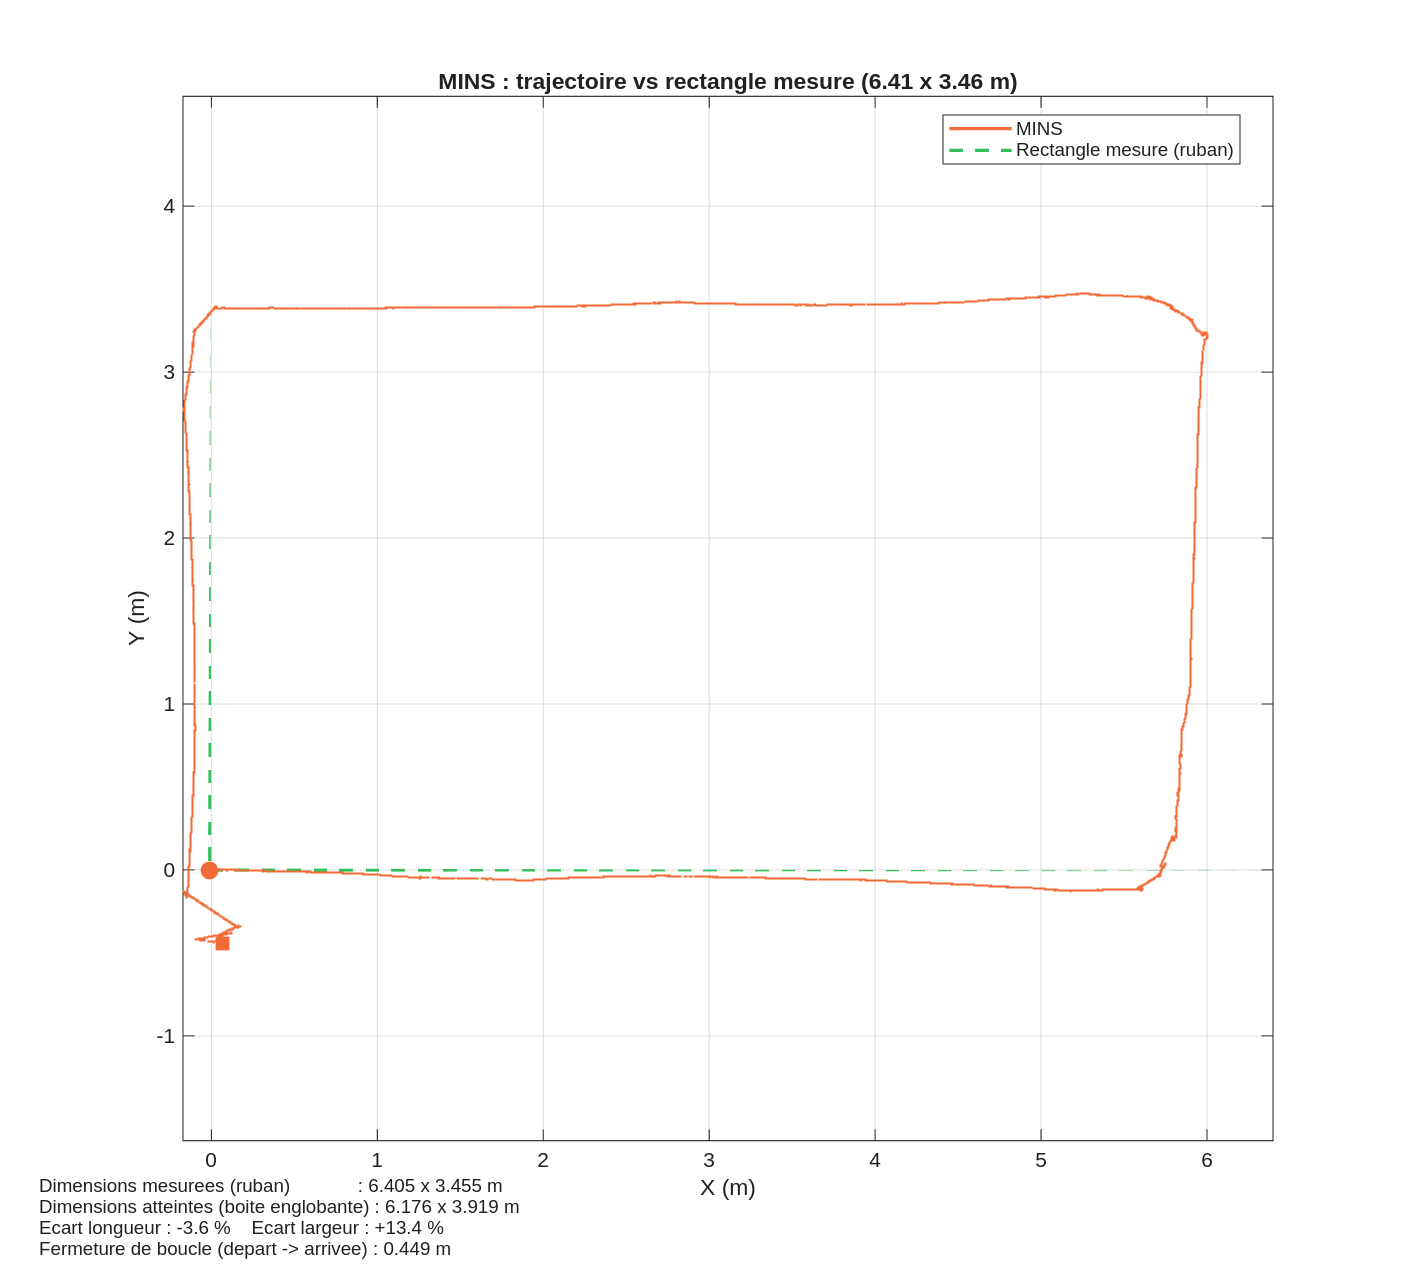
\includegraphics[width=0.72\linewidth]{figures/rect_test_aug05_mins.png}
\caption{MINS against the taped $6.405\,\text{m}\times3.455\,\text{m}$
rectangle, 2026-08-05, produced by
\code{plot\_rectangle\_test('test1', 6.405, 3.455, 'mins')}
(\S\ref{ap:repro-mins-guide}). Bounding box $6.176\times3.919$\,m
($-3.6\,\%$ / $+13.4\,\%$); loop closure $0.449$\,m over a $23.35$\,m path
($1.9\,\%$); heading drift over the full loop $5.1^\circ$.}
\label{fig:aug05mins}
\end{figure}
The length error is small and one-sided ($-3.6\,\%$); the width error is
larger and one-sided the other way ($+13.4\,\%$). Table~\ref{tab:aug05calib}
gives the more likely reading over a pure scale error: this platform's
turning asymmetry (\S\ref{sec:aug05calib}) accumulates differently depending
on which way the rover turns at each corner, so a rectangle driven
consistently anticlockwise does not distort its two axes equally. A coarse,
purely qualitative read of the raw trajectory against elapsed time
(Table~\ref{tab:aug05progress}; not a validated per-corner algorithm, offered
only as a description of what the logged points show) is consistent with
that reading: distance from the start point falls to a local minimum near
$t=159$\,s, just after the rectangle's third corner, before drifting further
to the final $0.449$\,m over the last leg.

\begin{table}[htbp]
\centering\small
\begin{tabular}{rrrr}
\toprule
$t$ (s) & $x$ (m) & $y$ (m) & dist. from start (m) \\
\midrule
0   & $-0.01$ & $-0.00$ & $0.01$ \\
79  & $+5.79$ & $+3.38$ & $6.71$ \\
133 & $-0.10$ & $+3.25$ & $3.25$ \\
159 & $-0.06$ & $-0.21$ & $0.21$ \\
213 & $+0.06$ & $-0.44$ & $0.45$ \\
\bottomrule
\end{tabular}
\caption{Raw trajectory progression, 5 of 9 sampled instants. Qualitative
motivation for \S\ref{sec:aug05beacon} only.}
\label{tab:aug05progress}
\end{table}

openVINS did not close the same rectangle. The same physical loop, recorded
in the same rosbag, gave a $675.28\times96.01$\,m bounding box and a
$2760.55$\,m path against a $19.72$\,m measured perimeter ---
$140\times$ over. Figure~\ref{fig:aug05compare}, produced by
\code{compare\_tests.m}, puts both laps on one figure.

\begin{figure}[htbp]
\centering
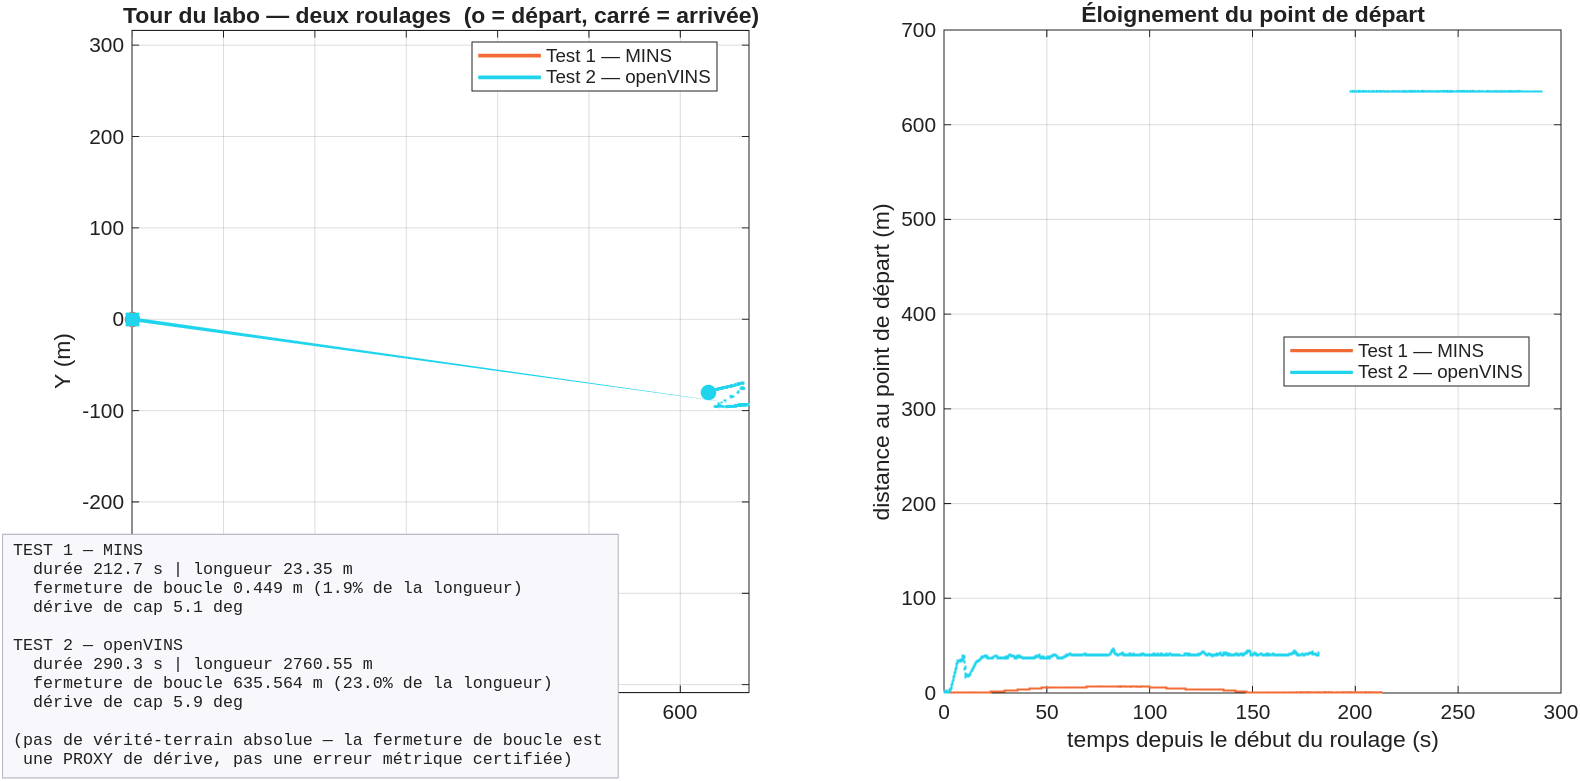
\includegraphics[width=0.95\linewidth]{figures/rect_test_aug05_compare.png}
\caption{\code{compare\_tests('test1','test2')}: MINS (Test 1, trusted) and
openVINS (Test 2, trusted) against the same physical loop. Left: both
trajectories, one axis. Right: distance from the starting point over time
--- openVINS climbs to a plateau near $40$\,m within the first $20$\,s, then
jumps once, near $t\approx190$\,s, to the $635$\,m range and holds there for
the remainder of the recording.}
\label{fig:aug05compare}
\end{figure}

\paragraph{A single scale factor cannot rescue this trajectory, and the check
is worth showing in full.} If openVINS's error were pure uniform scale, some
constant $k$ would bring every axis into agreement simultaneously. Solving
for $k$ from each dimension independently,
\begin{equation}
k_L = \frac{6.405}{675.28} = 0.00948, \qquad
k_W = \frac{3.455}{96.01}  = 0.03598, \qquad
k_P = \frac{19.72}{2760.55} = 0.00714,
\label{eq:scalecheck}
\end{equation}
gives three factors disagreeing by up to $3.8\times$ ($k_W/k_L$). Applying
$k_L$ alone, the value that makes the length exact by construction, to every
axis: length lands on target by definition, but width becomes $0.911$\,m
against a $3.455$\,m target ($-73.6\,\%$), and the loop-closure gap becomes
$6.028$\,m --- thirteen times \emph{worse} than MINS's $0.449$\,m, not
better. This is a deformation of the trajectory's shape, not a resizing of
it, and no single number corrects it (\S\ref{sec:july29align} makes the
identical point about scale hiding inside an alignment-based metric, from
the other direction).

Nearly identical heading drift over the two independent loops --- $5.1^\circ$
MINS, $5.9^\circ$ openVINS, from the same \code{compare\_tests.m} run above
--- says the same thing from a second angle: an estimator whose orientation
tracking were fundamentally broken would show it here too. openVINS's
failure this session is concentrated in scale, not in heading, matching the
open question already on record for this platform
(\S\ref{sec:july29align}: ``openVINS's scale disagrees with itself between
runs''), and matching a result this platform \emph{has} produced under
better conditions: $0.025$\,m loop closure, $0.1\,\%$, on 2026-07-29
(\S\ref{sec:july27twotest}), the same estimator, the same rover, an
$86^\circ$C Pi rather than $89$--$90^\circ$C and a lit, textured floor rather
than the dim underside of furniture. The comparison in this section is
between a completed acquisition and a failed one, not a fair contest between
two algorithms on equal footing; \S\ref{tab:openitems} records what
completing it fairly would require.

\subsection{A second absolute-error method: paired sightings, no anchor
required}
\label{sec:aug05beacon}
\S\ref{ap:repro-absolute}'s beacon bridge gives a continuous absolute error
once anchored, but is gated on the colour camera's intrinsics, which remain
uncalibrated at operating resolution (same section, opening trapbox): its
output today is smooth, repeatable, internally consistent and metrically
meaningless, the same phrase this report already uses for the identical
failure mode in a different context (\S\ref{sec:july30intrinsics}). Rather
than wait on that recalibration, this session added a second, complementary
method built on hardware already trusted for a different purpose: the
infrared stereo pair, already Kalibr-calibrated to $0.20$--$0.23$\,px
(\S\ref{ap:repro-calib}) because openVINS and MINS both depend on it, and
already running AprilTag detection at $\sim\!5$--$6$\,Hz for the corridor
markers (\S\ref{ap:trap-diffdrive}).

\paragraph{The measurement principle.} Suppose a fixed AprilTag is sighted
twice, at times $t_a$ and $t_b$, and its position in the camera frame is the
same at both instants to within a small tolerance $\varepsilon$:
$\lVert\mathbf{c}(t_a)-\mathbf{c}(t_b)\rVert \le \varepsilon$. Because the tag
has not moved, this means the \emph{camera} was in the same place at both
instants, to the same tolerance. If $\hat{\mathbf p}$ denotes the pose an
estimator reports, a perfect estimator would then satisfy
$\hat{\mathbf p}(t_a) = \hat{\mathbf p}(t_b)$; the observed difference,
\begin{equation}
\varepsilon_{\text{drift}} \;=\; \bigl\lVert \hat{\mathbf p}(t_b) -
\hat{\mathbf p}(t_a) \bigr\rVert ,
\qquad
\text{given}\ \ \lVert\mathbf{c}(t_a)-\mathbf{c}(t_b)\rVert \le \varepsilon ,
\label{eq:tagdrift}
\end{equation}
is drift accumulated between the two sightings. Crucially, Eq.~\ref{eq:tagdrift}
never needs the tag's true position in the world, nor the camera--IMU
extrinsic connecting the detection to \code{base\_link}: both would be
needed to say \emph{where} the beacon is, but Eq.~\ref{eq:tagdrift} only ever
asks whether the rover was in the same place twice. This is the same relation
the ground-truth panel's rotation maneuvers already exploit in one dimension
(depart and return to a marked heading); here it is a free-standing check at
any point in a longer loop, not only at the loop's own start and end.
\begin{center}
\begin{tikzpicture}[font=\scriptsize, scale=0.95,
  cn/.style={draw, circle, fill=black!4, minimum size=5mm},
  bn/.style={draw, diamond, fill=accentblue!15, draw=accentblue, minimum size=7mm}]
% Rectangle drawn slightly larger than the two sighting markers below need,
% so the tag and both robot positions each get clear room for their own
% label -- the earlier version packed all three into the corner itself and
% the labels overlapped.
\draw[thick] (0,0) rectangle (6.4,3.46);
\node[cn] (start) at (0,0) {};
\node[below right=1pt] at (start) {\footnotesize start/finish};
\draw[->, accentblue, thick] (6.4,0) -- (6.4,3.46) -- (0,3.46);
\draw[->, accentblue, thick] (0,3.46) -- (0,0) -- (6.4,0);
\node[bn] (beacon) at (0.55,3.46) {};
\node[above=2pt] at (beacon) {\footnotesize fixed tag, corner 3};
% ra/rb well separated (>2 units) with labels routed to opposite sides,
% specifically so neither the markers nor their captions can touch --
% a tighter first attempt made both ambiguous at print resolution.
\node[cn, fill=alertred!25, draw=alertred] (ra) at (0.45,2.35) {};
\node[left=2pt] at (ra) {\footnotesize $t_a$, lap 1};
\node[cn, fill=alertred!25, draw=alertred] (rb) at (2.55,1.15) {};
\node[right=2pt] at (rb) {\footnotesize $t_b$, lap 2};
\draw[<->, alertred, thick, dashed] (ra) -- node[above, sloped, pos=0.5]{$\varepsilon_{\text{drift}}$} (rb);
\end{tikzpicture}
\end{center}

\paragraph{Why the third corner, and why an observation, not a correction.}
Table~\ref{tab:aug05progress} places the point of closest apparent approach
to the start near the \emph{third} corner, one leg before the final,
largest-error segment; a fixed reference there can tell whether that
near-closure was genuine convergence or coincidence, which the single
end-to-end loop-closure number in \S\ref{sec:aug05result} cannot. The tag is
therefore placed to be sighted once per lap at that corner, across several
laps of the same rectangle.

What Eq.~\ref{eq:tagdrift} is not is a way to zero the estimator's state at
that corner. Doing so was considered and rejected: snapping the pose to a
known value at each corner would make the driven trajectory match the
rectangle \emph{by construction}, exactly the failure this report already
names when it happens elsewhere --- ``smooth, repeatable, internally
consistent and metrically meaningless'' (\S\ref{ap:repro-absolute}) applies
here word for word. \code{/tag\_detections} is instead recorded into the same
detached rosbag as every other topic
(\code{ROBUST\_REC\_TOPICS}, \code{leo\_backend.py}) purely as an observation
channel, wired into nothing that reads or writes the estimator's state.
\code{tools/tag\_drift.py} performs Eq.~\ref{eq:tagdrift} entirely offline,
after the fact, pairing sightings of the same tag ID separated by at least
$5$\,s (so a sighting is never compared against itself) and within
$\varepsilon=5$\,cm of each other in camera coordinates by default. Verified
against a synthetic pair of sightings carrying a known $0.264$\,m drift
before being run on real data: the tool reads back $0.264$\,m exactly.
Camera-frame AprilTag positions also feed
\code{plot\_rectangle\_test.m}'s figures directly, marking both where the
rover stood at each sighting and, separately, the tag's own deduced position
--- the latter derived through the documented tape-measure camera extrinsic
(\code{T\_imu\_cam}, \S\ref{ap:repro-mins-guide}) rather than a Kalibr
solution, so it is offered as
a visual aid, while the \emph{spread} between repeated deductions of one
physical tag remains meaningful regardless: the tag has not moved, so any
spread is drift by Eq.~\ref{eq:tagdrift}, independent of how well the
extrinsic locates it in an absolute sense.

\begin{trapbox}{This method has not yet measured anything}
Everything above is implemented, tested against synthetic data with a known
answer, and deployed: the detector, the recording, the CSV format, and
\code{tag\_drift.py} itself. What has not happened yet is placing a tag at
the rectangle's third corner and driving multiple laps past it --- every
number in Eq.~\ref{eq:tagdrift}'s worked example above is synthetic, chosen
to exercise the tool, not a field measurement. The first real run belongs in
this trapbox once it exists, not before.
\end{trapbox}

\section{Open items registry}
\label{sec:openitems}
\small
\begin{center}
\begin{longtable}{@{}cL{6.2cm}L{6.8cm}@{}}
\caption{Explicit registry of placeholders and pending decisions.}
\label{tab:openitems} \\
\toprule
\# & Item (status) & Required action \\
\midrule
\endfirsthead
\multicolumn{3}{l}{\tablename\ \thetable{} (continued)} \\
\toprule
\# & Item (status) & Required action \\
\midrule
\endhead
\midrule
\multicolumn{3}{r}{continued on next page} \\
\endfoot
\bottomrule
\endlastfoot
1 & \textbf{Rigid-wheel radius/track} (config frozen at stock values;
    2026-07-21: leftward drift measured directly, $\approx 1.65\,\%$
    right/left effective-radius bias (\S\ref{sec:yawtrim}); masked in
    software by a bisected yaw trim, $K\approx-0.087$\,rad/s per m/s, not a
    substitute for the measurement below) &
    roll-out measurement; update firmware \code{diff\_drive} and
    \code{config\_wheel.yaml}; re-run slip protocol; remove the software
    trim (\S\ref{sec:yawtrim}) once corrected \\
2 & \code{T\_imu\_cam} (measured seed, refined online) &
    \code{kalibr\_calibrate\_imu\_camera} (monocular cam0), inject via
    \code{fill\_mins\_camchain.py} \\
3 & TF \code{base\_link$\to$camera/laser} (placeholders) &
    calliper/CAD measurement; must agree with item 2 \\
4 & Camera frame-rate margin: \textbf{10\,Hz option CANCELLED}
    (2026-07-08) & the D455 does \emph{not} support 640$\times$480@10
    (supported: 6/15/30/60/90); the attempted change silently disabled all IR
    streams (driver fell back to a depth-only default profile) and caused a
    full vision outage until reverted. Lesson: validate any profile change
    against \code{rs-enumerate-devices} before deployment. 15\,Hz retained;
    real-time margin to be sought elsewhere (feature floor, budget
    acceptance). \\
5 & Carolus / fixed-AprilTag global anchor (VICON slot staged) &
    enable ladder stage 3: drift-free global updates inside MINS \\
6 & RPLidar (node down) & bring-up, scan$\to$cloud conversion, extrinsic \\
7 & AprilTag size cross-check & compare tag range against checkerboard range
    at identical position \\
8 & \code{leo\_autonomy} package (SLAM/exploration, written \& built) &
    install dependencies, remap \code{cmd\_vel} through \code{twist\_mux},
    field trial \\
9 & Zombie-guard false positives under Wi-Fi roaming (\S
    \ref{sec:corridorvalidation}): \code{leo\_watchdog.sh} restarted the full
    stack every 1--3\,min throughout the July 20 traverse; debounce widened
    (3$\to$6 ticks, 10$\to$20\,s) but not yet re-validated in motion.
    July 22 (\S\ref{sec:july22network}): restarts observed recurring at an
    exact 6-minute cadence over an 18-minute window, i.e.\ every single
    debounce tick failing with zero resets in between, sustained loss of
    registration visibility rather than isolated roaming blips &
    repeat an in-motion traverse with the widened debounce and confirm the
    false-trigger rate drops; if it persists, replace the \code{rosnode
    list} round trip with a check that does not require a live RPC to the
    robot's master while roaming \\
10 & Watchdog liveness checks test node \emph{presence}, not topic
    \emph{output} (\S\ref{sec:jointstates}): \code{firmware\_message\_converter}
    stayed registered while silently producing zero \code{/joint\_states}
    messages, blocking MINS indefinitely with no alert. \textbf{Recurred
    July 22} (\S\ref{sec:july22network}), same node, same symptom, same
    fix, this time costing $\approx$2\,h of network-focused misdiagnosis
    before being recognised as the same fault, since the recommended fix
    below was still not implemented &
    add an output-rate probe (e.g.\ zero-publisher or stalled-rate detection
    on \code{/joint\_states}) alongside the existing presence checks,
    now confirmed by a second occurrence to be worth the implementation
    cost \\
11 & Unbounded ``still starting'' grace period in the web healer
    (\S\ref{sec:july21}): a stuck rosbridge TLS process was left alone for
    hours because idempotency has no time ceiling &
    add a maximum grace duration, past which an unbound port is treated as
    failed rather than starting, and the process is killed and relaunched \\
12 & WireGuard tunnel failure that outlived every restart tried
    (\S\ref{sec:wgroam}): endpoint roaming (Eq.~\ref{eq:roam}) explained and
    fixed the first occurrence, but a second, unrelated failure resisted
    restarts on both ends, a port change, and a 4-minute idle wait, while
    ICMP/SSH to the robot stayed healthy throughout. A milder recurrence
    was observed July 22 (\S\ref{sec:july22network}): a $\approx$15\,s
    reachability loss that self-recovered without intervention &
    obtain campus-side firewall/NAT logs for the failure window if
    possible; otherwise instrument the tunnel with a lighter-weight
    same-subnet fallback (\S\ref{sec:samesubnet}) as a permanent, not just
    emergency, option \\
13 & Ground-station Wi-Fi (\code{rtl88x2bu}) is back on the critical path
    (\S\ref{sec:samesubnet}) whenever the same-subnet fallback is in use,
    reintroducing the driver fault Ethernet was originally chosen to avoid
    (\S\ref{sec:network}) &
    replace the adapter (Intel/MediaTek chipset) so the same-subnet path is
    not gated by known-defective hardware \\
14 & Discontinuous, roughly one-second-burst motion reported during the
    July 21 traverse: the dominant cause is now identified and fixed
    (\S\ref{sec:manualdeadman}, the manual-drive deadman tripping under
    operator-device Wi-Fi roaming); the pose-availability floor
    ($A_{\text{pose}}\gtrsim 0.85$, \S\ref{sec:traverseoutcome}) and an
    unmeasured Wi-Fi image-bandwidth risk remain as secondary, undistinguished
    contributors, mainly to the separately-reported missed-obstacle symptom &
    re-validate the deadman fix over a full traverse; trace
    \code{/joint\_states} and image-topic Hz directly on the Pi, timestamped
    against restart\_stack.sh's own init log, to attribute any remaining
    roughness to pose gaps, image starvation, or both \\
15 & AUTO mode control-loop hardening (\S\ref{sec:automode}: patrol-steering
    EMA, avoidance-direction EMA, lock hysteresis, \code{DEPTH\_ALIVE\_TIMEOUT})
    deployed but not yet validated over a full traverse: the test window
    that would have exercised it was consumed by the disk-full incident
    (\S\ref{sec:diskcrash}); the July 22 session (\S\ref{sec:july22}) added
    further, still-unvalidated hardening to the same loop, dual-confirmation
    beacon reset and a first PID retrofit (items 17--18 below) &
    repeat an AUTO-mode traverse once network conditions are ordinary;
    confirm the depth-alive gate actually fires (not just compiles) by
    forcing a depth-topic stall while facing a wall \\
16 & Robot disk usage is unmonitored until a downstream symptom (camera
    failures that resist hardware reset) reveals it indirectly
    (\S\ref{sec:diskcrash}); \code{leo.service} has no restart policy, so a
    crash (SIGSEGV observed, root cause unconfirmed, plausibly a
    disk-full write failure) stays dead until noticed by hand &
    add a disk-usage probe to \code{leo\_watchdog.sh} (warn well before
    100\,\%; the \code{/var/ros/log} growth alone justifies a periodic
    purge); add \code{Restart=on-failure} to \code{leo.service} so a future
    crash self-heals like every other component in this architecture \\
17 & Three PID loops (\S\ref{sec:pid}) deployed live but not yet exercised
    over a full AUTO traverse under ordinary network conditions
    (\S\ref{sec:pidvalidation}); no gain is derived from a plant model of
    this rover, every gain is either reused unchanged from a field-tuned
    predecessor or, for the obstacle governor (no predecessor existed),
    chosen from a geometric margin argument rather than measured response &
    a traverse confirming the intended qualitative effect (smoother patrol
    heading, earlier and smoother wall-approach deceleration) without new
    oscillation; if warranted, a measured step-response or frequency-domain
    characterisation of at least the obstacle governor to replace the
    margin-based $K_p$ (Eq.~\ref{eq:obstfloor}) with a derived one \\
18 & Dual LED+checkerboard confirmation (\S\ref{sec:dualconfirm}) assumes
    the two cues are simultaneously valid at some reachable pose; not yet
    confirmed against this beacon's actual physical layout. If structurally
    impossible (checkerboard readable only from a face where the LEDs are
    not bright enough, or vice versa), \code{DUAL\_CONFIRM\_GRACE\_S} will
    expire on every attempt and no beacon will register autonomously &
    bench-test at the intended stop distance whether \code{led\_stable} and
    \code{lm\_hits} (\S\ref{sec:automode}'s vision-loop counters) both cross
    their confirmation thresholds at any single pose before relying on this
    gate in an unattended traverse \\
19 & Pi$\leftrightarrow$CORE2 serial link (\code{serial\_node},
    250{,}000\,baud) logged 20{,}295 checksum/lost-sync errors in 2\,h on
    July 22 (\S\ref{sec:july22network}), the leading, plausible-but-unproven
    hypothesis for why \code{firmware\_message\_converter}'s wheel
    subscription failed at its most recent onset; independent of item 10's
    watchdog blind spot and unresolved by this session's fix. \textbf{Still
    active July 23}: a live measurement during this session's audit read
    $\approx$200 errors/min, worse than the July 22 figure, not better &
    a measurement tool (\code{tools/check\_serial\_health.sh}) and a
    physical-inspection checklist (\code{tools/diag\_serial\_pi\_core2.md})
    now exist so a before/after comparison is possible; physically inspect
    the Pi$\leftrightarrow$CORE2 connector/cable for a marginal connection
    per that checklist \\
20 & \code{ov\_msckf} (VINS) found not running at all (no process) during
    July 22 verification of \S\ref{sec:july22tf2}'s unrelated MINS/tf2\_ros
    change; removes the VINS fallback until restarted, cause and onset time
    not established. \textbf{Addressed July 23}: \code{leo\_watchdog.sh} now
    carries a presence check for \code{/ov\_msckf}, symmetric to
    \code{mins\_subscribe}'s (same 6-tick debounce, same
    \code{restart\_stack.sh} remedy) &
    not yet field-validated against a real VINS dropout — the original
    incident was never reproduced under controlled conditions, so the new
    check's effectiveness is inferred from symmetry with MINS's, not
    directly observed \\
21 & Return-to-Base's full-trajectory retracing (\S\ref{sec:july23rtb},
    Eq.~\ref{eq:rtbwaypoints}). \textbf{Exercised July 24}: multiple live
    multi-waypoint retraces occurred (Table~\ref{tab:rtblog}), exposing a
    genuine safety gap — the reverse leg had no obstacle or stall detection
    of any kind (\S\ref{sec:july24rtb}) — now closed by a two-tier guard
    plus a graduated resistance/obstacle governor
    (\S\ref{sec:july24rtbfix}--\S\ref{sec:july24rtbgrad}) &
    a further live traverse specifically exercising the new guard's
    graduated response (Eq.~\ref{eq:rtbresistscale}), not just its two hard
    trips, which Table~\ref{tab:rtblog}'s single post-fix run already
    exercised once \\
22 & The initial-divergence guard's threshold
    (\code{MAX\_INITIAL\_JUMP\_M}$=5$\,m, Eq.~\ref{eq:initguard},
    \S\ref{sec:july23guard}) is a bench choice from a single observed
    incident (VINS at $27.5$\,m), not a derived or measured bound &
    characterise against a real distribution of clean vs.\ divergent VINS
    initialisations across multiple sessions before treating $5$\,m as more
    than a first cut \\
23 & The deterministic $35^\circ$-left avoidance policy
    (\S\ref{sec:july24avoid}, Eq.~\ref{eq:avoidcumulative}) has not been
    exercised against a corridor obstructed specifically on the left, the
    scenario in which up to three cumulative left turns are attempted
    toward the blocked side before the $180^\circ$ U-turn fallback
    (\code{AVOID\_MAX\_TRIES}$=3$) rescues it &
    a live trial in a room with a known left-side obstruction (a doorway
    or corridor bend), confirming the U-turn fallback engages within the
    expected three attempts and that no contact occurs during them \\
24 & The 20th-percentile threshold replacing the median for direction
    selection (\S\ref{sec:july24percentile}, Eq.~\ref{eq:percentilebias})
    is a bench choice reasoned from first principles (a point between the
    existing $q=50$ and $q=5$ statistics), not fit to a measured
    distribution of real obstacle occupancy fractions $f$ &
    log $f$ (fraction of near-range pixels) for real obstacles encountered
    over several sessions and confirm $q=20$ remains above the smallest
    $f$ actually observed in practice \\
25 & The RTB resistance-governor thresholds
    ($\rho_{\text{lo}}=0.35$, $\rho_{\text{hi}}=0.75$, Eq.~\ref{eq:rtbresistscale})
    and the stall detector's window/displacement pair
    ($T_{\text{stall}}=2.0$\,s, $d_{\text{stall}}=3$\,cm, Eq.~\ref{eq:rtbstalltrip})
    are reasoned against the platform's known static noise floor
    (Table~\ref{tab:t11}) but not tuned against a live distribution of
    genuine partial-resistance events (wheel slip, minor snags) &
    collect $\rho[k]$ (Eq.~\ref{eq:rtbresistratio}) over several ordinary
    RTB runs with no actual obstruction, to confirm the ratio stays above
    $\rho_{\text{hi}}$ under normal reversing and the governor does not
    fire spuriously \\
26 & \code{BOOST\_ANG}$=0.9$\,rad/s (\S\ref{sec:july24boost},
    Eq.~\ref{eq:boostvalues}) is inferred from
    \S\ref{sec:precision-campaign}'s ramp characterisation, which measured
    yaw authority only up to $0.40$\,rad/s commanded, not from a ramp
    measurement at boost-level commands themselves &
    repeat \code{tools/ramp\_yaw.py}'s protocol with commands spanning
    \code{BOOST\_ANG}, confirming authority does not degrade (or
    quantifying by how much it does) above the previously characterised
    range \\
27 & The widened LED area window $(3,2500)$\,px$^2$
    (\S\ref{sec:july24range}, Eq.~\ref{eq:ledratio}) clears the derived
    $64\times$ ratio for the requested $0.5$--$4$\,m range but is reasoned
    from a single 1\,m calibration point, not measured at either end of
    the range itself &
    capture and replay real frames at 0.5\,m and at 4\,m through the
    offline LED detector (the method that already resolved
    \S\ref{sec:beacon-closed}), confirming the widened bounds pass the
    genuine beacon without admitting new false positives \\
28 & \code{BEACON\_SPATIAL\_MAX\_FRAC}$=1.5$
    (\S\ref{sec:july24spatial}, Eq.~\ref{eq:spatialscale}) bounds the
    LED/checkerboard separation ratio conservatively above the beacon's
    true physical $s_{\text{gap}}/s_{\text{cb}}$, which has not itself
    been measured on the physical beacon &
    measure the beacon's actual LED-cluster-centre to
    checkerboard-centre offset and width directly, and tighten the
    fraction toward the measured ratio if margin allows \\
29 & \code{ov\_msckf} (VINS) still builds against the deprecated ROS1
    \code{tf} package (\code{ROS1Visualizer.\{h,cpp\}},
    \code{ROSVisualizerHelper.h}, \S\ref{sec:july24tf2}), the same class
    of debt \S\ref{sec:july22tf2} closed for MINS on July 22; isolated via
    \code{/tf\_vins} (harmless today) but not yet ported &
    mirror \S\ref{sec:july22tf2}'s field-for-field port against the same
    upstream \code{ROS2Visualizer.\{h,cpp\}} template already used for
    MINS \\
30 & No \code{map} frame or \code{map}$\to$\code{odom} transform exists
    anywhere in the shared \code{/tf}; the mission's world-referenced
    concepts (RTB, obstacle/beacon mapping) instead consume a parallel,
    non-TF SE(2) state (\code{world\_origin\_x/y}, \code{world\_heading},
    Eq.~\ref{eq:worldse2}, \S\ref{sec:july24tf2}) re-anchored by hand at
    each beacon reset &
    implement the sketched \code{tf2\_ros.TransformBroadcaster}-based
    \code{map} publisher (\S\ref{sec:july24tf2}) and migrate
    \code{\_get\_world\_pos()}'s callers to
    \code{tf2\_ros.Buffer.lookup\_transform()}; nontrivial (multiple call
    sites across RTB/mapping/LOCK) and not attempted on the live robot
    without a dedicated validation pass \\
31 & The re-armed pose-source switch's automatic-apply path
    (\S\ref{sec:july24switch}: \code{\_on\_odom()} completing an armed
    switch on a source's first message) is verified by code inspection and
    by a manual arm/cancel round trip only, not by an actual drive that
    lets an armed, previously-silent source publish and confirms the
    switch fires without operator action &
    arm VINS while stationary, then drive to give it motion, and confirm
    both the \topic{pose\_source} and \topic{pose\_source\_pending} topics
    (and the cockpit buttons) transition automatically at the same instant
    \code{/ov\_msckf/odomimu} starts publishing \\
32 & \code{navigation\_supervision.launch}'s \code{pose\_selector}
    \code{default\_source} was corrected from \code{"VINS"} to
    \code{"MINS"} (\S\ref{sec:july24switch}) after the wrong default
    silently dropped \code{/robot\_pose\_fused} to zero on a live restart;
    the fix is in the launch file but not yet on the running parameter
    server, which still holds \code{"VINS"} from the stack's last full
    launch &
    confirm \code{default\_source} reads \code{"MINS"} on
    \code{/pose\_selector} after the next full stack restart
    (\code{restart\_stack.sh} or \code{leo start}), not merely a single
    node respawn \\
33 & \code{VioManager::vio\_alive()} and \code{is\_initialized\_vio}'s
    \code{std::atomic<bool>} conversion (\S\ref{sec:july24vinsdebug}) are
    real, independently-justified fixes but were found and verified
    against a filter that had not itself initialised this session
    (\S\ref{sec:july24vinsdebug}'s log-attribution correction); neither
    has been observed live doing the one thing it was designed for —
    keeping odometry served once \code{ov\_msckf} initialises and then
    goes (or stays) stationary &
    after a live jerk-triggered initialisation succeeds
    (Table~\ref{tab:openitems}, item 31's drive trial covers getting
    there), let the rover sit still afterward and confirm
    \code{/ov\_msckf/odomimu} keeps publishing rather than stopping once
    ZUPT starts succeeding on every frame \\
34 & The trajectory-comparison pipeline (\S\ref{sec:july27pipeline}) and its
    Figure~\ref{fig:trajcomparison} slot are validated only on a stationary
    bench capture (MINS at rest, VINS uninitialised, no beacon); no real
    driven MINS-versus-VINS overlay with VINS initialised, and no
    Carolus-referenced error figure, has yet been produced &
    drive a manual loop with VINS initialised (item 31's jerk) past a
    Carolus beacon, run \code{record\_trajectories.sh} $\rightarrow$
    \code{bag\_to\_csv.py} $\rightarrow$ \code{plot\_trajectories.m}, and
    drop the resulting \code{figures/traj\_comparison.png} into the report
    to replace the placeholder \\
35 & The two-test protocol of \S\ref{sec:july27twotest}
    (Figure~\ref{fig:testcomparison}, \code{compare\_tests.m}) is built and
    verified against synthetic data only; the closing analysis of
    \S\ref{sec:july27twotest} is fully scaffolded with \code{\textbackslash
    todo\{\}} placeholders but has no real numbers, because the two drives
    it depends on (Test 1 under MINS, Test 2 under openVINS, same lab loop)
    have not yet been run &
    drive Test 1 and Test 2 from the cockpit Trajectory tab per
    \S\ref{sec:july27twotest}'s protocol, run \code{compare\_tests()}, and
    fill in every \code{\textbackslash todo\{\}} in
    \S\ref{sec:july27twotest} from its printed output \\
36 & \textbf{Colour-camera intrinsics do not match the operating stream}
    (\S\ref{sec:july30intrinsics}), \textbf{BLOCKING}.
    \code{carolus\_astrobee\_rex} runs with $f_x=644.12$, $c_x=643.47$,
    $c_y=372.52$, calibrated at $1280\times720$, against a $640\times480$
    stream whose own \code{camera\_info} reports $f_x=380.35$,
    $c_x=320.40$, $c_y=243.72$. The principal point falls outside the
    image; the two configurations differ in field of view
    ($90^\circ$ versus $\approx80^\circ$) and are not related by any scale
    factor. A target at the true image centre is reported $26.7^\circ$
    off-axis (Eq.~\ref{eq:july30bearingerror}) &
    re-run the colour intrinsic calibration at $640\times480$, the
    resolution actually published, and load the result into the detector.
    \textbf{No dimensional metric (absolute error, range, beacon
    position) may be published from this camera until this is done.}
    This gates items 37 and 5 \\
37 & \textbf{Beacon-anchored absolute error: architecture complete, never
    recorded} (\S\ref{sec:july30bridge}). \code{carolus\_tf\_bridge.py}
    publishes \code{/odom\_in\_beacon} and \code{/carolus\_in\_beacon},
    which together give an absolute error with no fitted transform and no
    scale freedom, superseding the Kabsch/Umeyama residuals of
    \S\ref{sec:july29align}. It has been run and observed to publish, but
    no bag recorded to date contains either topic &
    once item 36 is cleared, record a driven run with both topics in the
    bag and report their instantaneous difference; this is the measurement
    the whole comparison programme has been building toward \\
38 & \textbf{Thermal envelope is three degrees wide}
    (\S\ref{sec:july30thermal}). The July 28 scheduling fix holds the
    serial link at $86\,^\circ$C under full colour load ($19.7$\,Hz wheel
    odometry, $82.8$\,Hz IMU) and does not hold it at $89.1\,^\circ$C,
    where the chain collapses entirely ($676\,751$ UART overruns, load
    $8.85$, all firmware topics at $0$\,Hz). A targeted \code{rosmon}
    cycle recovers it, but the overrun counter resumes climbing at once
    ($+553$ in three minutes) &
    install active cooling; the colour nodelet's measured $185\,\%$ CPU is
    the dominant thermal term, so the alternative is to give up colour and
    with it the working-distance beacon detection. Re-measure the envelope
    after cooling: the correct A/B experiment is overrun rate at fixed
    load, not temperature alone \\
39 & \textbf{Second absolute-error method: implemented, never measured}
    (\S\ref{sec:aug05beacon}). Item~37's beacon bridge is gated on
    item~36; this session added a complementary method on already-
    calibrated hardware (the Kalibr'd IR pair, item~2) that needs
    neither the tag's world position nor the camera--IMU extrinsic, only
    a fixed tag re-sighted from the same spot. The detector, the
    recording path, the CSV format and \code{tools/tag\_drift.py} are
    all deployed and verified against synthetic data with a known
    answer; no tag has yet been placed at the rectangle's third corner
    for a real multi-lap run &
    mount an AprilTag at a fixed, re-visitable point (the rectangle
    protocol's third corner is already instrumented for it,
    \S\ref{ap:repro-mins-guide}); drive at least two laps past it in one
    recording; run \code{tag\_drift.py} on the result \\
\end{longtable}
\end{center}

\FloatBarrier
In summary, the campaign transformed the estimation layer from a divergent
prototype into a measured, guarded and self-healing system, quantified end to
end: millimetric planar stability, bounded vertical noise, a real-time visual
front-end within $2\times$ of its budget floor, and an operator platform whose
every indicator is backed by a live topic. July 24's session closes the
campaign's remaining collision-safety blind spot: every branch capable of
commanding forward motion in AUTO mode now carries both a hard obstacle
check and a graduated speed governor (Table~\ref{tab:speedaudit}), including
the one direction the depth sensor cannot observe at all, where an
odometry-inferred stall detector and resistance governor
(\S\ref{sec:july24rtbfix}--\S\ref{sec:july24rtbgrad}) now stand in for the
sensing that physically cannot exist. The remaining precision and validation
roadmap is fully enumerated in Table~\ref{tab:openitems}, with the rigid-wheel
radius re-measurement (item 1) and a live trial of the deterministic
avoidance policy against a left-blocked corridor (item 23) the
highest-priority metrological and safety actions respectively.
